% ------------------------------------------------------------------------
% ------------------------------------------------------------------------
% ICMC: Modelo de Trabalho Acadêmico (tese de doutorado, dissertação de
% mestrado e trabalhos monográficos em geral) em conformidade com 
% ABNT NBR 14724:2011: Informação e documentação - Trabalhos acadêmicos -
% Apresentação
% ------------------------------------------------------------------------
% ------------------------------------------------------------------------

% Opções: 
%   Qualificação          = qualificacao 
%   Curso                 = doutorado/mestrado
%   Situação do trabalho  = pre-defesa/pos-defesa (exceto para qualificação)
%   Versão para impressão = impressao
\documentclass[mestrado]{packages/icmc}

% ---------------------------------------------------------------------------
% Pacotes Opcionais
% ---------------------------------------------------------------------------
\usepackage{rotating}           % Usado para rotacionar o texto
\usepackage[all,knot,arc,import,poly]{xy}   % Pacote para desenhos gráficos
% Este pacote pode conflitar com outros pacotes gráficos como o ``pictex''
% Então é necessário usar apenas um dos pacotes conflitantes
\newcommand{\VerbL}{0.52\textwidth}
\newcommand{\LatL}{0.42\textwidth}
% ---------------------------------------------------------------------------
%\usepackage{eucal}
%\usepackage[mathcal]{eucal}
\usepackage[mathscr]{eucal}
\usepackage{tikz}
\usetikzlibrary{quotes, angles, intersections}
\usepackage{enumitem}

\renewcommand{\algorithmicrequire}{\textbf{Input:}}
\renewcommand{\algorithmicensure}{\textbf{Output:}}

%\usepackage{algorithm2e}

%MEUS COMANDOs

\newtheorem{theorem}{Theorem}

\newcommand{\R}{\mathbb{R}}
\newcommand{\Co}{\mathbb{Co}}
\newcommand{\D}{\mathscr{D}}
\newcommand{\Pp}{\mathscr{P}}
\newcommand{\Cc}{\mathscr{C}}
\newcommand{\E}{\mathscr{E}}
\newcommand{\Ww}{\mathscr{W}}
\newcommand{\Rr}{\mathscr{R}}
\newcommand{\norm}[2][2]{\left\lVert#2\right\rVert_{#1}}

\newcommand{\IncFig}[1]{
	\def\svgwidth{\columnwidth}
	\import{./figures/}{#1.pdf_tex}
}

\newcommand{\bigO}{\mathscr{O}}
%\newcommand{\fautor}{\legend{Reference: Made by the author.}}

%siglas
\newcommand{\MCLP}{MCLP}
\newcommand{\PMCLP}{PMCLP}
%\usepackage{import}
%\usepackage{xifthen}
%\usepackage{pdfpages}
\usepackage{transparent}
\usepackage{multirow}
\usepackage{siunitx}
\sisetup{group-separator = {,}}

%FIM MEUS COMANDOS

% ---
% Informações de dados para CAPA e FOLHA DE ROSTO
% ---
% Tanto na capa quanto nas folhas de rosto apenas a primeira letra da primeira palavra (ou nomes próprios) devem estar em letra maiúscula, todas as demais devem ser em letra minúscula.
\tituloPT{Cobertura Planar Maximal por Elipses}
\tituloEN{Planar Maximal Covering with Ellipses}
\autor[Tedeschi, D. F.]{Danilo Françoso Tedeschi}
\genero{M} % Gênero do autor (M = Masculino / F = Feminino)
\orientador[Orientadora]{Profa. Dra.}{Marina Andretta}
%\coorientador{Prof. Dr.}{Fulano de Tal}
\curso{CCMC}
\data{01}{03}{2019} % Data do depósito
\idioma{EN} % Idioma principal do documento (PT = português / EN = inglês)
% ---


% ---
% RESUMOS
% ---

% Resumo em PORTUGUÊS
% conter no máximo 500 palavras
% conter no mínimo 1 e no máximo 5 palavras-chave
%\textoresumo[brazil]{
 %   Este trabalho é um breve modelo  para a escrita de monografias de qualificação, dissertações e teses utilizando o ambiente \LaTeX, de acordo com as normas exigidas pelo Instituto de Ciências Matemáticas e de Computação (ICMC), da Universidade de São Paulo (USP). Para a confecção deste modelo foi utilizado a última versão (1.9.6) do pacote de classes \textit{abnTeX2} que segue as normas da Associação Brasileira de Normas Técnicas. A elaboração de uma monografia, dissertação ou tese pode ser feita sobrescrevendo o conteúdo deste modelo. 
 %   }{Modelo, Monografia de qualificação, Dissertação, Tese, Latex}


% resumo em INGLÊS
% conter no máximo 500 palavras
% conter no mínimo 1 e no máximo 5 palavras-chave
\textoresumo[english]{
    Planar maximal covering with ellipses is an optimization problem where one wants to place ellipses on the plane to cover demand points, such that a function depending on the value of the covered points and on the cost of the ellipses that have been used is maximized. Initially, we developed an algorithm for the version of the problem where the ellipses are parallel to the coordinate axis. For the future, we intend to adapt an approximation algorithm developed for the planar maximal covering by disks and develop a method for the variant of the problem where the ellipses can be freely rotated. 
    }{Optimization, Planar Maximal Covering Location Problem, maximal covering of points using ellipses}

% ----------------------------------------------------------
% ELEMENTOS PRÉ-TEXTUAIS
% ----------------------------------------------------------

% Inserir a ficha catalográfica
%\incluifichacatalografica{tex/pre-textual/ficha-catalografica.pdf}

% DEDICATÓRIA / AGRADECIMENTO / EPÍGRAFE
%\textodedicatoria*{tex/pre-textual/dedicatoria}
%\textoagradecimentos*{tex/pre-textual/agradecimentos}
%\textoepigrafe*{tex/pre-textual/epigrafe}

% Inclui a lista de figuras
\incluilistadefiguras

% Inclui a lista de tabelas
%\incluilistadetabelas

% Inclui a lista de quadros
%\incluilistadequadros

% Inclui a lista de algoritmos
\incluilistadealgoritmos

% Inclui a lista de códigos
%\incluilistadecodigos

% Inclui a lista de siglas e abreviaturas
%\incluilistadesiglas

% Inclui a lista de símbolos
%\incluilistadesimbolos

% ----
% Início do documento
% ----
%\tracingmacros=1
\begin{document}
% ----------------------------------------------------------
% ELEMENTOS TEXTUAIS
% ----------------------------------------------------------
\textual

\chapter{Introduction}
\label{chapter:introduction}
Two main types of optimal covering problems can be found in the literature: the Minimum Cover Problem, also known as just Set Cover Problem, and the Maximal Covering Problem \cite{karatas}. 

One of the 21 Karp's NP-Complete problems\footnote{The decision version, which asks if there is a cover of size $k$, is NP-Complete.} \cite{karp}, the Minimum Cover Problem is very well explored and considered to be a classic. 
Given a demand set and collection of subsets of the demand set, the problem asks what is the minimum number of elements from the collection of subsets needed to cover the whole demand set. One of its most famous examples is the Minimum Vertex Cover defined over graphs, where the vertex set has to be covered by a subset of edges.

The second type of covering problems arose from the fact that covering almost all the demand set can be a lot cheaper than having to cover it all \cite{garcia}. This second type is known as \sigla{\MCLP}{Maximal Covering Location Problem} and was introduced in \cite{church:1974}. In this first study, it is defined on a network with demand nodes, a facility set is also given and a solution maximizes the demand coverage satisfying the constraint that only a subset of the facilities is used. Just like the Minimum Cover, MCLP is a NP-Hard problem \cite{hatta:2013} and both deterministic, (using integer programming) \cite{church:1974}, and heuristic methods \cite{revelle:2008} have been proposed to solve it.

In \cite{church:1984} a new kind of MCLP named \sigla{\PMCLP}{Planar Maximal Covering Location Problem} was introduced. This version of the problem was not defined on a network, instead the demand set and the facilities are located in $\R^2$ having the coverage area of a facility be defined by a distance function. PMCLP is said to have been studied under Euclidean and rectilinear distance functions \cite{younies}. The Euclidean norm PMCLP, which has a lot of results that can be applied for the elliptical PMCLP, is also found in the literature as the problem of maximization of points covered by a fixed number of unit disks \cite{cabello:2006}. 
Early works only tackled the one-disk version of the problem, in \cite{chazelle:1986} a $\bigO(n^2)$ algorithm, which still stands as the best in terms of run-time complexity, was proposed besting the prior $\bigO(n^2\log{n})$ algorithm created by \cite{drezner}.
The $m$ unit disks maximal covering was studied in \cite{cabello:2006} which had as its most important result a $(1-\epsilon)$-approximation algorithm which runs in $\bigO(n\log{n})$. To achieve its main goal, however, they developed a deterministic $\bigO(n^{2m-1}\log{n})$ algorithm which gets employed into their approximation scheme.
Additionally, in \cite{aronov:2008} one-disk maximal covering is proven to be 3SUM-HARD. This means that maximizing the amount of points covered by a disk is as hard as finding three real numbers that sum to zero among $n$ given real numbers.

Planar maximal covering with ellipses differs from its disks counterpart only in the shape of the facility's coverage area. The main motivation to study this modified version is that cellphone towers can have elliptical shaped coverage area, so in order to determine what are the best locations to place $m$ cellphone towers to maximize the amount of the population covered by its signal, an elliptical PMCLP is better suited \cite{canbolat}. Only two articles have been found published in the literature that study this problem. In \cite{canbolat}, a mixed non-linear programming method was proposed as a first approach to the problem. For some instances the method took too long and did not find the optimal solution. For this reason a heuristic method was developed using a technique called Simulated Annealing, solutions for the instances that timed-out with the first method were then obtained. The problem was further explored in \cite{andreta} which proposed a deterministic method that showed better performance obtaining the optimal solutions for the instances which the first method could not. Also, in \cite{andreta}, a version of the problem where every ellipse can be freely rotated was introduced and an exact method, which could not find the optimal solutions for large instances, and a heuristic method were proposed for it. Despite the similarities, none of the works cited above base their development on the maximal covering with disks algorithms found in the literature.


This work is structured in the following way: \autoref{chapter:definitions} introduces some definitions and results that are used throughout the next chapters; in \autoref{chapter:pmclp}, the maximal covering by disks problem is studied and a $\bigO(n^{2m})$ algorithm is proposed; in \autoref{chapter:ellipses}, the maximal covering by ellipses is introduced and the algorithm for the disks case is adapted for it; finally, \autoref{chapter:future_work} presents what is left as future work. Also, \autoref{chapter:ellipses_intersection} determines with detail the intersection of two ellipses, which is used in the algorithm developed in \autoref{chapter:ellipses}.



\chapter{Notation and Preliminaries}
\label{chapter:definitions}
Some definitions and results that are used throughout the text are given in this chapter.

\section{Norm}

A norm is a function that maps every vector from a vector space onto a non-negative real number satisfying some conditions. Here it is defined for the vector space $\R^2$ as follows

\begin{definicao}
Let $\xi : \R^2 \mapsto [0, \infty]$, $\xi$ is said to be a norm function of $\R^2$ if for any $p, q \in \R^2$ and $a \in \R$,

\begin{enumerate}
    \item $\xi(p + q) \le \xi(p) + \xi(q)$
    \item $\xi(ap) = |a|\xi(p)$
    \item if $\xi(p)=0$, then $p=0$
\end{enumerate}

\end{definicao}

\subsection{Elliptical and euclidean norm functions}

Let $u \in \R^2$ be a vector, the euclidean norm of $u$ is defined as

\begin{equation}\label{eq:norm2}
||u||_2 = \sqrt{u^{T}u}
\end{equation}

The elliptical norm takes a $2$ by $2$ positive definite matrix as its parameter. This matrix can be seen as a linear transformation of the euclidean norm. Let $u \in \R^2$ be a vector and $Q$ be a $2$ by $2$ positive definite matrix, the elliptical norm of $u$ is defined as 

\begin{equation}
||u||_{elliptical} = \sqrt{u^{T}Qu}
\end{equation}

It is easy to see that the elliptical norm, when taking $Q$ to be the identity matrix, becomes the euclidean norm.

Determining the distance between two points, given a norm function is done by calculating the norm of the vector defined by the difference between the two points. For example, the elliptical distance between the points $p,q \in \R^2$ is given by $||p-q||_{elliptical}$.

\section{Disk}

A circle (or circumference) is a set of points in $\R^2$ that have constant euclidean distance, also known as radius, to another point, also referred to as the center of the circle. A unit circle is a circle with radius equal to $1$.
A disk is the set of points bounded by a circle, in other words let $c \in \R^2$, a unit disk with center $c$ is the set of every point $p \in \R^2$ which satisfy \autoref{eq:disk}.

\begin{equation}\label{eq:disk}
||p-c||_2^2 \le 1
\end{equation} 

\section{Ellipse}

The ellipse is a curve which is categorized, along with the parabola and the hyperbola, as a conic section. As the name suggests, conic sections are curves resulted from the intersection of a right circular cone in $\R^3$ with a plane \cite{brannan:geometry}. From that definition, an equation which describes any conic section is given as follows

\begin{equation}\label{equation:quadratic_form}
Ax^2 + Bxy + Cy^2 + Dx + Ey + F = 0
\end{equation}

To distinguish an ellipse from the other conic sections given an instance of \autoref{equation:quadratic_form}, the condition $4AC - B^2>0$ can be verified \cite{ayoub}.

Assuming the center of an ellipse is $c \in \R^2$, then \autoref{equation:quadratic_form} can be rewritten as a quadratic form as follows

\begin{equation}
(p-c)^{T}Q(p-c) = 1
\end{equation}

with $p \in \R^2$ and $Q$ being a $2$ by $2$ positive definite matrix which carries the parameters of the ellipse. From \autoref{equation:quadratic_form}, $Q$ can be defined as follows

\[
Q=
\left( {\begin{array}{cc}
	A & \frac{B}{2} \\
	\frac{B}{2} & C \\
	\end{array} } \right).
\]

Note that asking $Q$ to be positive definite is the same as asking $4AC-B^2$ to be positive. This makes us arrive at the following definition of the ellipse

\begin{definicao}\label{def:ellipse}
    Let $c\in \R^2$ be the center of an ellipse and $Q$ be a $2$ by $2$ positive definite matrix, an ellipse is the set of every point $p \in \R^2$ that have $||p-c||_{elliptical}^2 = (p-c)^{T}Q(p-c) = 1$. Also, a point $p$ is considered covered by an ellipse if $||p-c||_{elliptical}^2 = (p-c)^{T}Q(p-c) \le 1$.
\end{definicao}

An alternative way to define an ellipse, which can be seen as just a property derived from the definition above, is to begin its construction with two points called foci and a constant $R \in \R$, with $R$ being greater than the euclidean distance between the two foci points (see \autoref{fig:ellipse_with_foci}). The ellipse is, then, defined as the set of points whose distance to the foci is equal to $R$. In other words, let $f_1, f_2 \in \R^2$ be the two foci points, the ellipse is the set of every point $p \in \R^2$, such that $||p-f_1||_2 + ||p-f_2||_2 = R$. It can be shown that this definition is equivalent to \autoref{def:ellipse}, with the coverage of a point $p$ being equivalent to $||p-f_1||_2 + ||p-f_2||_2 \le R$.

\begin{figure}[H]
    \centering
    
    \caption{A non-axis-parallel ellipse and its foci points.}
    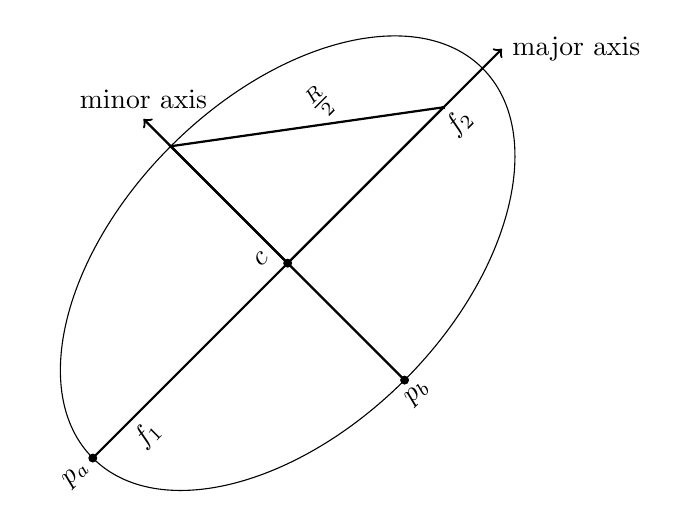
\begin{tikzpicture}[xscale=0.7, yscale=0.7][domain=0:11]
   % \draw [help axis] (-5,-3) grid (5,3);

    \begin{scope}[rotate=45]
    \draw (0,0) ellipse (5cm and 3cm);
    \node[rotate=45][below] at (-4,0) {$f_1$};
    \node[rotate=45][below] at (4,0) {$f_2$};
    \draw[fill] (-4,0) circle [radius=.5pt];
    \draw[fill] (4,0) circle [radius=.5pt];
    \draw [thick] (4,0) -- (0,0) -- (0,3) -- (4,0);
    \draw[->,thick] (-5,0)--(5.5,0) node[right]{major axis};
    \draw[->,thick] (0,-3)--(0,3.7) node[above]{minor axis};
        \node[rotate=45] [left] at (0,0.4) {$c$};
    \node [rotate=45][right] at (2.1,1.65) {$\frac{R}{2}$};
    
   
    \node [rotate=45][left] at (-5,0) {$p_a$};
    \draw[fill] (-5,0) circle [radius=2pt];
    
        \draw[fill] (0,0) circle [radius=2pt];
    
    \draw[fill] (0,-3) circle [radius=2pt];
    \node [below][rotate=45] at (0,-3) {$p_b$};
    \end{scope}

    %a^2-b^2=c^2 -> c^2=25-9=16 -> c=4
    
    %\draw[fill] (0,0) circle [radius=.5pt];
	
    %
    %\draw[fill] (5,0) circle [radius=1pt];
    %\draw[fill] (0,3) circle [radius=1pt];
    %
    

    %\node [below] at (2.1,0) {$c$};
	%\node [left] at (-0.1,1.5) {$b$};



    %\node [above] at (5,0) {$(x_0+a,y_0)$};
    %\node [above] at (-5,0) {$(x_0-a,y_0)$};
    %\node [above] at (0,3) {$(x_0,y_0+b)$};
    %
    

    
    %\draw [-] (-5,0) -- (5,0);
     %\draw [-] (0,-3) -- (0,3);
     %\draw [|-|] (0.001,-0.1) -- (4.999,-0.1);
\end{tikzpicture}
    \fautor
    \label{fig:ellipse_with_foci}
\end{figure}

Also, in \autoref{fig:ellipse_with_foci}, the distance $a = ||p_a - c||_2$ is called the semi-major, and the distance $b = ||p_b-c||_2$ is called the semi-minor. These two values are also referred to as the shape parameters of an ellipse. Let $d = ||c-f_1||_2$, then it is easy to see that $a = R - d$ and $b = \sqrt{\frac{R^2}{4} - d^2}$.

Finally, an ellipse is said to be axis-parallel if its major-axis (see \autoref{fig:ellipse_with_foci}), which is the line that passes through its two foci points, is parallel to the $x$-axis.

\subsection{Axis-parallel}

An axis parallel ellipse centered at $c = (c_x,c_y)$ can be described using \autoref{def:ellipse} with $Q$ being a diagonal matrix \footnote{The only non-zero terms are in the main diagonal}. This can be understood as a scaling transformation applied to the euclidean norm.
Defining the matrix $Q$ as

\[
Q=
\left( {\begin{array}{cc}
    \frac{1}{a^2} & 0 \\
    0 & \frac{1}{b^2} \\
    \end{array} } \right)
\]

Then, starting from \autoref{def:ellipse}, we can obtain the following equation

\begin{align*}
        (p-c)^{T}Q(p-c) = 1\\
    (\frac{p_x-c_x}{a^2}, \frac{p_y-c_y}{b^2})^{T}(p_x-c_x, p_y-c_y) = 1
 \end{align*}
 \begin{equation}\label{equation:pellipse}
  \frac{(p_x-c_x)^2}{a^2} + \frac{(p_y-c_y)^2}{b^2} = 1
 \end{equation}

where $a$ and $b$ are the semi-major and semi-minor shape parameters respectively.

Also, the coverage region is determined by just changing the equality to a inequality as follows

\begin{equation}\label{equation:cover_pellipse}
\frac{(p_x-c_x)^2}{a^2} + \frac{(p_y-c_y)^2}{b^2} \le 1
\end{equation}

Another way to represent ellipses, which will be useful in some occasions, is through writing it as a curve, function of the angle with its major-axis (see \autoref{fig:ellipse_params}).

\begin{figure}[H]
    \centering
    
    \caption{The ellipse as a parametric curve}
    

%\tikzset{every picture/.style={line width=0.75pt}} %set default line width to 0.75pt        

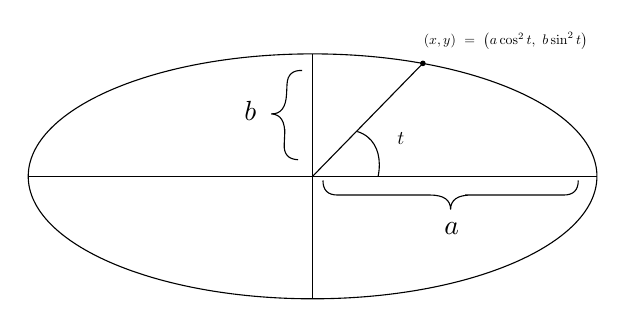
\begin{tikzpicture}[x=0.75pt,y=0.75pt,yscale=-1,xscale=1]
%uncomment if require: \path (0,300); %set diagram left start at 0, and has height of 300

%Shape: Ellipse [id:dp1559950964552308] 
\draw   (100,180) .. controls (100,147.42) and (161.34,121) .. (237,121) .. controls (312.66,121) and (374,147.42) .. (374,180) .. controls (374,212.58) and (312.66,239) .. (237,239) .. controls (161.34,239) and (100,212.58) .. (100,180) -- cycle ;
%Straight Lines [id:da3716259356733107] 
\draw    (100,180) -- (374,180) ;


%Straight Lines [id:da9880464900454329] 
\draw    (237,121) -- (237,239) ;


%Shape: Brace [id:dp3973633345998604] 
\draw   (242,182) .. controls (242,186.67) and (244.33,189) .. (249,189) -- (293.5,189) .. controls (300.17,189) and (303.5,191.33) .. (303.5,196) .. controls (303.5,191.33) and (306.83,189) .. (313.5,189)(310.5,189) -- (358,189) .. controls (362.67,189) and (365,186.67) .. (365,182) ;
%Shape: Brace [id:dp94498526835576] 
\draw   (232,129) .. controls (227.34,128.79) and (224.9,131.01) .. (224.68,135.67) -- (224.47,140.23) .. controls (224.16,146.89) and (221.68,150.11) .. (217.01,149.9) .. controls (221.68,150.11) and (223.85,153.55) .. (223.54,160.21)(223.68,157.21) -- (223.33,164.68) .. controls (223.12,169.35) and (225.34,171.79) .. (230,172) ;
%Shape: Arc [id:dp3154280429415799] 
\draw  [draw opacity=0] (258.54,158.43) .. controls (260.37,158.96) and (262.06,159.82) .. (263.54,161.03) .. controls (268.5,165.07) and (270.12,172.1) .. (268.62,179.79) -- (244.51,184.38) -- cycle ; \draw   (258.54,158.43) .. controls (260.37,158.96) and (262.06,159.82) .. (263.54,161.03) .. controls (268.5,165.07) and (270.12,172.1) .. (268.62,179.79) ;
%Shape: Circle [id:dp8908034615999807] 
\draw  [fill={rgb, 255:red, 0; green, 0; blue, 0 }  ,fill opacity=1 ] (289.08,125.57) .. controls (289.08,124.98) and (289.56,124.51) .. (290.14,124.51) .. controls (290.73,124.51) and (291.21,124.98) .. (291.21,125.57) .. controls (291.21,126.16) and (290.73,126.64) .. (290.14,126.64) .. controls (289.56,126.64) and (289.08,126.16) .. (289.08,125.57) -- cycle ;
%Straight Lines [id:da6323920079482996] 
\draw    (290.14,125.57) -- (237,180) ;



% Text Node
\draw (304,205) node   {$a$};
% Text Node
\draw (207,148.33) node   {$b$};
% Text Node
\draw (330,114.67) node [scale=0.5]  {$( x,y) \ =\ \left( a\cos^{2} t,\ b\sin^{2} t\right)$};
% Text Node
\draw (279.6,162) node [scale=0.7]  {$t$};


\end{tikzpicture}

    \fautor
    \label{fig:ellipse_params}
\end{figure}

Let $c \in \R^2$ be the center of an ellipse with shape parameters $(a,b) \in \R^2_{>0}$. Then $\gamma : [0, 2\pi] \mapsto \R^2$ defines a curve which maps every angle onto a point on the ellipse and it is defined as follows

    \begin{equation}\label{eq:parametric_ellipse}
    \gamma(t) = \left\{
    \begin{array}{l}
    x(t)= a\cos{t} + c_x\\
    y(t)=b\sin{t} + c_y
    \end{array}
    \right.
    \end{equation}

No equivalent disk-circle wording exists for ellipses, this could be a source of ambiguity in the text, that is why a note for the reader was judged to be necessary. Throughout this work an ellipse will represent the set of points that satisfy \autoref{def:ellipse}. In some places, though, with prior clarification, we will denote as an ellipse, the set of points that are covered by the ellipse itself. For example, when we define $\Pp \cap E$ as the set of points in $\Pp$ that are covered by $E$, we are implicitly calling $E$ the set of points that are covered by the ellipse itself as it is defined by \autoref{def:ellipse}.

\chapter{Maximum Covering by Disks}
\label{chapter:pmclp}
In this chapter, we introduce a version of the classical Euclidean norm PMCLP where each facility has a given coverage radius. 
We refer to this problem as \sigla{MCD}{Maximum Covering by Disks}. We also propose a method for it intending to adapt it for the elliptical PMCLP that will be introduced in the next chapter. 

\section{Definition}

An instance of MCD is given by a set of $n$ demand points $\Pp:=\{p_1, \dots, p_n\}$, with $p_j\in\R^2$; a set of weights $\Ww:=\{w_1, \dots, w_n\}$, with $w_j\in\R_{\ge0}$ being the weight of point $p_j$; and $m$ disks given by their radii $\Rr:=\{r_1, \dots, r_m\}$, with $r_j\in\R_{>0}$. 
Additionally, to make the text more clear, we define a set of $m$ disks as $\D:=\{D_1, \dots, D_m\}$, with $D_j : \R^2 \mapsto \R^2$ being a function that takes the center where the $j$-th disk is located as input, and returns its coverage region as defined by \autoref{eq:disk}.

A solution for an instance of MCD is determined by $Q:=(q_1, \dots, q_m) \in \R^{2m}$ which specifies the center of every disk in $\D$.
The coverage region of the $j$-th disk centered at $q_j$ is denoted by $D_j(q_j)$. Finally, let $w : 2^{\Pp} \mapsto \R_{\ge0}$ be the function

\begin{equation}\label{eq:subset_w}
w(A) = \sum_{j : p_j \in A} w_j,
\end{equation}
which takes a subset of $\Pp$ and returns the sum of the weights of every point in it; then an optimal solution of MCD is given by the optmization problem:

\begin{equation}
\max_{Q} w\left(\bigcup_{j=1}^m \Pp \cap D_j(q_j)\right).
\end{equation}

As a remark, it is important to note that MCD is a slightly different PMCLP than the one introduced in the first study on the subject in \citeonline{church:1984}. There, a coverage radius is given for each demand, rather than for each facility, and a demand is only considered covered if a facility is located within its radius.

\subsection{CLS and CIPS}

The method proposed in \citeonline{church:1984} involves the creation of a \sigla{CLS}{Candidate List Set}, which is a finite set of possible solutions, for each facility. After a CLS is constructed, a complete search can be executed to find the best solution.

As this work is developed towards the creation of an exact method for MCD, the focus is on constructing a CLS that contains an optimal solution.
This is done in \citeonline{church:1984} where a circle is defined for every demand point, and a \sigla{CIPS}{circle intersection point set} is constructed containing the demand points and every pairwise circle intersection.
Here, we introduce a similar approach based on works found on the case for only one disk and describe a $\bigO(n^2\lg{n})$ algorithm for it.

\section{Related Work}
In \citeonline{cabello:2006}, a $\bigO(n^{2m-1}\log{n})$ algorithm for $MCD$ is developed as a sub-routine for its $(1-\epsilon)$-approximation algorithm. Firstly, they solve a sub-problem for two disks in $\bigO(n^3\log{n})$. Then, for the rest of the points that are not in that solution, it uses the algorithm developed in \citeonline{chazelle:1986} for the one-disk case, checking every possible solution for every one of the disks left.

Also, in \citeonline{zhou} an heuristic method for large-scale $MCD$ is proposed. It uses a probabilistic algorithm called mean-shift which is a gradient ascent method proven to converge to a local density maxima of any probability distribution. The mean-shift is utilized to find good candidates of centers for the unit disks, then the method backtracks to find the best assignment. The results showed that the greedy algorithm achieves an optimal coverage in some instances, but for some other ones it has a 15 percent worse coverage ratio.

\section{One disk version}

This version of the problem will be refered to as \sigla{MCD-1}{Maximum Covering by One Unit Disk} and it is just a specific case of MCD with only one disk with radius one ($m=1$ and $r_1=1$). We later use the algorithm for MCD-1 here described to construct a CLS which is guaranteed to contain an optimal solution for MCD.

Two exact methods for MCD-1 have been found in the literature. A $\bigO(n^2)$ algorithm is proposed by \citeonline{chazelle:1986} which improved the previously $\bigO(n^2\log{n})$ one proposed by \citeonline{drezner}.
As it has been mentioned, MCD-1 is a 3SUM-HARD problem, which means that it is as hard as the 3SUM problem (the problem of finding three real numbers that sum to zero, given $n$ real numbers). Initially the lower bound of the 3SUM problem was conjectured to be $\Omega(n^2)$, matching the best algorithm for MCD-1, which meant that no better time-complexity could be achieved. Since then, however, better algorithms for 3SUM have been developed with a $\bigO(\frac{n^2}{poly(n)})$ run time complexity \cite{3SUM-kopelowitz:2014}.


In \citeonline{drezner}, the main idea used to develop the $\bigO(n^2\log{n})$ algorithm is that, even though there are infinitely many points where the disk could be placed, only a few of them, a finite amount of $\bigO(n^2)$, needs to be considered for the method to find an optimal solution.
The algorithm, for every point, sorts the other points with respect to the angle they form with the first one. After that, the first point is placed on the border of the disk and, going through the sorted list, the algorithm inserts and removes points from the disk coverage. Also, when inserting and removing a point from the coverage, it only checks the disk centers that make the entering/leaving point to be on the border. Because the algorithm only checks the centers that make the disk have two points on its border, the number of centers it goes through is bounded by the number of pairs of points, which is $\binom{n}{2} = \bigO(n^2)$.

In \citeonline{chazelle:1986} and \citeonline{cabello:2006}, on the other hand, instead of working directly with MCD-1, an equivalent problem called \sigla{MWC}{Maximum Weight Clique} was introduced. The algorithm for MCD that is developed in this chapter also uses that equivalence. Because of that, MWC is introduced in the next section.

\section{Maximum Weight Clique Problem}

An instance of MWC is given by a set of points $\Pp:=\{p_1,\dots,p_n\}$, with $p_i \in \R^2$; a set of unit disks $\D:=\{D_1(p_1),\dots,D_n(p_n)\}$; and a set of weights $\Ww=\{w_1, \dots, w_n\}$ with the $i$-th disk having a weight $w_i\in \R_{>0}$ assigned to it. To make the notation less cluttered, we use, in this problem, $D_j:=D_j(p_j)$, for $j\in\{1, \dots, n\}$.

A clique, in this context, is a non-empty intersection region of one or more disks, and its weight is the sum of the weights of those disks in the intersection.
Following this, a solution for MWC can be defined as just a point $q\in\cup_{j=1}^n D_j$ which is inside any of the given disks in $\D$.
From a solution $q$, the corresponding clique $S$ can be obtained by intersecting every disk that contains $q$:

\begin{equation}
S = \bigcap_{j : q \in D_j} D_j.
\end{equation}
With a geometric observation, though, the number of possible values for the solution can be reduced.
Let $\partial \D = \{ \partial D_1, \dots, \partial D_n \}$ be the set of circles corresponding to each disk in $\D$, it is possible to see that any clique has at least one point on its border that is in the intersection of two circles in $\partial D$ or, in the case where the clique is composed of only one disk, it contains the center of its only disk. Because of that, $q$ can be actually limited to the set of pairwise intersections of $\partial \D$ as well as the set of centers of each disk $\Pp$. Then, with this observation, an optimal solution of MWC can be defined by the optimization problem

\begin{equation}
\max_{q} \sum_{D_k \cap q \neq \emptyset} w_k,
\end{equation}
with $q \in \{\partial D_i \cap \partial D_j : 1 \le i < j \le n\} \cup \Pp$. With this new specification of the solution's search space, it can be shown that given an instance of MWC, an optimal solution for it can be found by going through $\binom{n}{2} + n = \bigO(n^2)$ possible ones.

It is worth pointing out that MWC is a different problem than the maximum clique on a intersection graph (a graph where the vertices are the disks and an edge exists if there is an intersection between two disks). 
As shown in \autoref{fig:three_disks_no_intersection}, three disks could have non-empty pairwise intersection and still have an empty intersection of all of them together.
That is why MWC is also referred to as the Maximum Geometric Clique Problem and the other version, when there is only the pairwise intersection condition, is referred to as the Maximum Graphical Clique Problem \cite{inplace:2014}. 

%The graphical version of the problem was studied by \citeonline{graphical-clique}, where a $\bigO(n^{4.5})$ algorithm was proposed. Also, in \citeonline{inplace:2014}, a $\bigO(n^2\log{n})$ time in-place algorithm\footnote{An in-place algorithm is an algorithm that needs $\bigO(1)$ extra space.} for arbitrary radii disks was proposed. 

In \citeonline{chazelle:1986}, the method for MWC consists on building a planar graph on which the vertices are the $\binom{n}{2}$ pairwise intersection of the circumferences and the edges are the arcs of the circumferences connecting the intersections. With the graph constructed, a traversal is done to obtain the answer, thus the time complexity of $\bigO(n^2)$.

\begin{figure}[H]
\centering

    \caption{Three disks that have non-empty pairwise intersection among them, but no common intersection.}
    %\begin{tikzpicture}[scale=1]
    %\draw [help lines] (-5,-3) grid (5,3);
    %\draw (0,0) circle (1cm) (0.9,1.6) circle (1cm) (-0.9,1.6) circle (1cm);

    %a^2-b^2=c^2 -> c^2=25-9=16 -> c=4
    
    %\draw[fill] (0.9,1.6) circle [radius=.5pt];
	%\draw[fill] (0,0) circle [radius=.5pt];
    %\draw[fill] (-0.9,1.6) circle [radius=.5pt];
    
    %\node[below] at (0,0) {$p_1$};
    %\node[below] at (0.9, 1.6) {$p_2$};
    %\node[below] at (-0.9, 1.6) {$p_3$};
    
    %\draw [-] (-5,0) -- (5,0);
     %\draw [-] (0,-3) -- (0,3);
     %\draw [|-|] (0.001,-0.1) -- (4.999,-0.1);
    %\end{tikzpicture}
       
    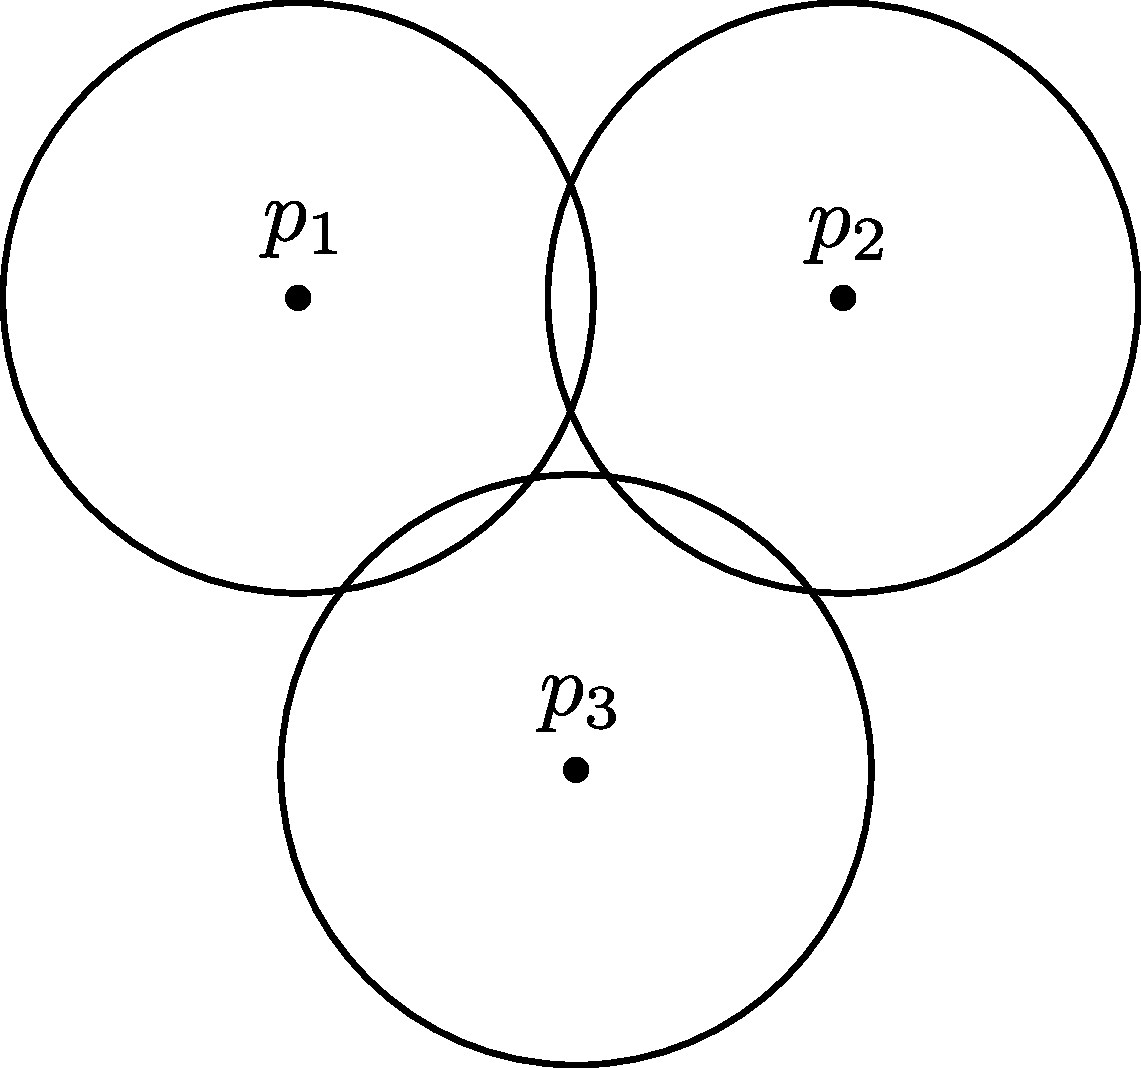
\includegraphics[scale=.35]{tex/figures/three_disks_no_intersection.pdf}
    \label{fig:three_disks_no_intersection}
    \fautor
\end{figure}

As it has been mentioned, with the equivalence of the two problems, an optimal solution of the Maximum Weight Clique Problem is also an optimal solution of MCD-1, which means that a disk centered at $q^*$ which is an optimal solution of MWC, will have a maximal weight covering of the demand set $\Pp$.

Given an instance of MCD-1, the equivalent MWC intance is obtained by defining the set $\D$ to contain the disks centered at $\Pp$ and setting the weight of every disk to be the weight of its corresponding point in $\Pp$. A disk $D_i$ will represent the area where a disk can be placed in order to cover $p_i$. This means that a intersection between some disks is a region where a disk could be placed to cover the corresponding points.

In \autoref{fig:three_disks_no_intersection}, it can be seen that there is no point where a disk could be placed such that it would cover $p_1, p_2$ and $p_3$, nonetheless, in any of the pairwise intersections, a disk could be placed to cover the two corresponding points.

Formally, in MWC, if a point $q$ lies inside $\bigcap_{k \in I} D_k$, with $I \subset \{1,\dots,n\}$, then a disk centered at $q$ will cover the points $p_k$, with $k\in I$ in the equivalent MCD-1 instance. Conversely, the same applies for a disk placed at $q$ that covers points $p_k$, with $k \in I$ in the MCD-1 instance. It means that $q$ will lie inside region $\bigcap_{k \in I} D_k$ in MWC.

\subsection{An algorithm for the Maximum Weight Clique Problem}

The algorithm described here is based on the one in \citeonline{drezner}, also with some ideas from \citeonline{inplace:2014} and \citeonline{cabello:2006}. It has a run time complexity of $\bigO(n^2\log{n})$ and uses $\bigO(n)$ of extra space. It is worth noting, however, that a $\bigO((n+K)\log{n})$ run time, with $K$ being the number of intersections, can be obtained by using the algorithm in \citeonline{bentley:1979} to find all the intersections among the $n$ circumferences.

In \citeonline{inplace:2014} an important observation is made about the intersection regions of disks. Given an instance of MWC, any clique formed by a subset of $\D$ is bounded by the arcs of circles that intersect with it. Also, those arcs have the intersection of circles as their end-points. This can be seen on \autoref{fig:3disks_intersect} where the cliques that $D_1$ is part of are bounded by $D_1$'s arcs which have its intersections with the other circles as end-points. Following this, a definition is presented to characterize the end-points of an arc bordering a clique.

\begin{definicao}\label{def:inter_arc}
    Let $D_i$ and $D_j$ be two unit disks with non-empty intersection, and $(\theta_1, \theta_2) \in [0,2\pi)^2$ be the two angles that $\partial D_i$ and $\partial D_j$ intersect, with the condition that $(\theta_1,\theta_2)$ defines an arc (counter-clockwise order) of $D_i$ that is the border of $D_i \cap D_j$. Then, define $\Gamma_+(i,j) = \theta_1$ and $\Gamma_-(i,j) = \theta_2$. For convenience, if $D_i$ is tangent to $D_j$, then $\theta_1=\theta_2$; and if $i=j$, then $\Gamma_-(i, j)=0$ and $\Gamma_+(i,j)=2\pi$.
\end{definicao}

\begin{figure}
\centering

    \caption{Three disks and their intersection points.}
    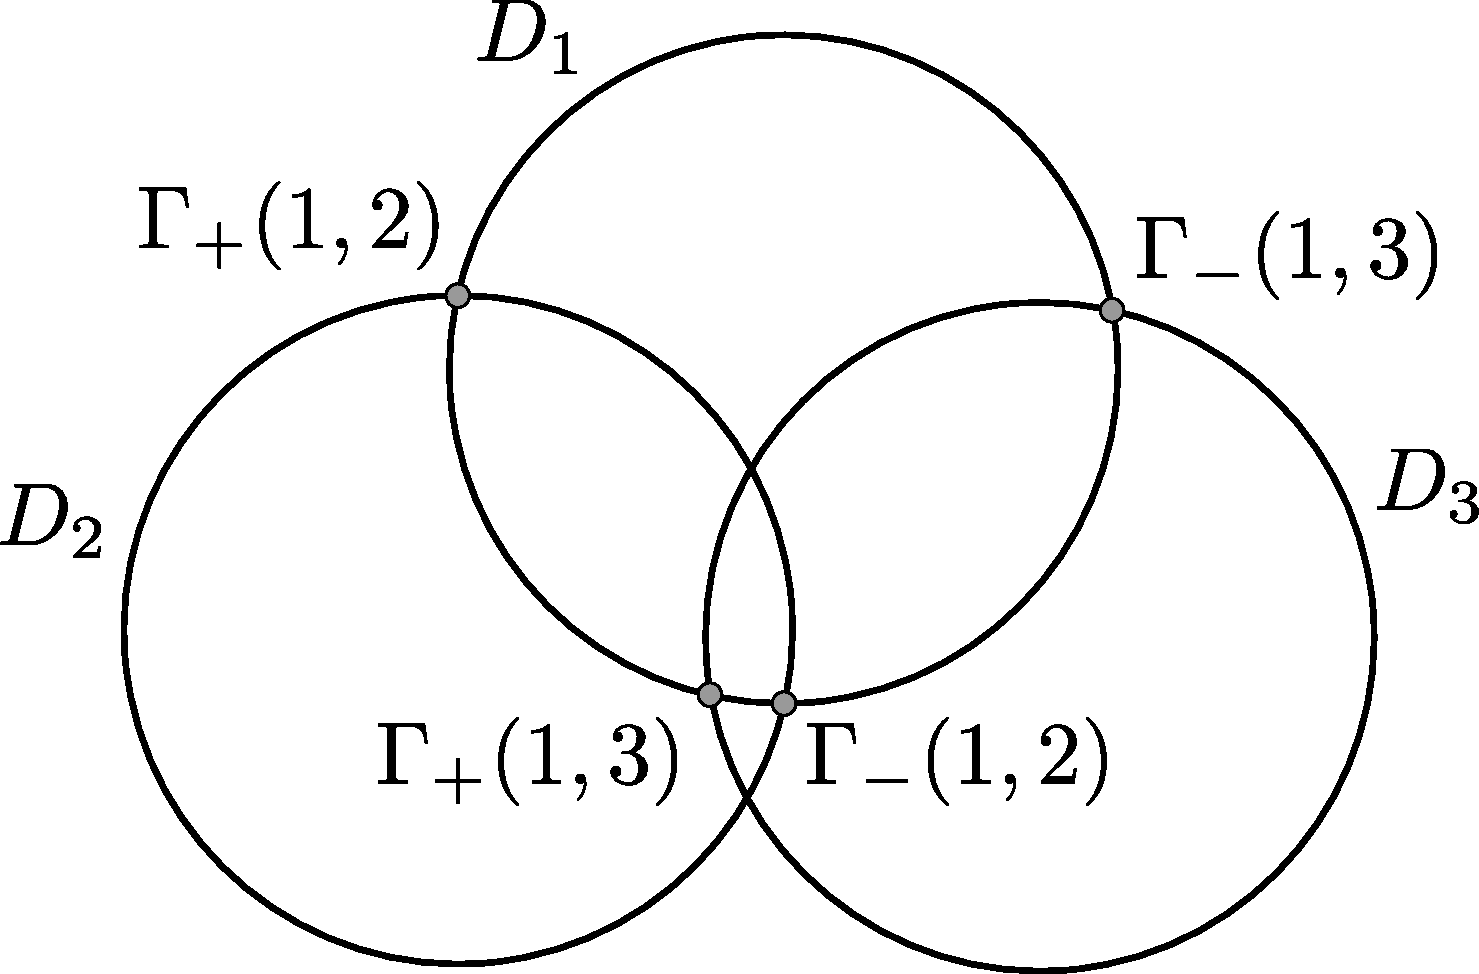
\includegraphics[scale=.36]{tex/figures/3_disks_intersect.pdf}
%    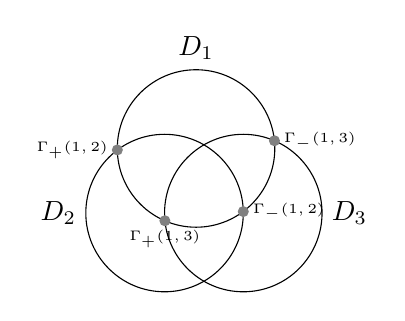
\begin{tikzpicture}
%\draw [help lines] (-5,-3) grid (5,3);

\draw[name path = c1] (0,0) circle (1cm);
\draw[name path = c3] (0.6,-0.82) circle (1cm);
\draw[name path = c2] (-0.4,-0.82) circle (1cm);

\node[above] at (0, 1) {$D_1$};
\node[left] at (-1.4, -0.82) {$D_2$};
\node[right] at (1.6, -0.82) {$D_3$};

\path [name intersections={of=c1 and c3}] ;
\foreach \i in {1,...,2}
\fill [color=gray] (intersection-\i) circle (2pt) ;

\node[right] at (intersection-1) {\tiny $\Gamma_-(1,3)$};
\node[left, below] at (intersection-2) {\tiny $\Gamma_+(1,3)$};

\path [name intersections={of=c1 and c2}] ;
\foreach \i in {1,...,2}
\fill [color=gray] (intersection-\i) circle (2pt) ;

\node[left] at (intersection-1) {\tiny $\Gamma_+(1,2)$};
\node[below,right] at (intersection-2) {\tiny $\Gamma_-(1,2)$};

%\draw [-] (-5,0) -- (5,0);
%\draw [-] (0,-3) -- (0,3);
%\draw [|-|] (0.001,-0.1) -- (4.999,-0.1);
\end{tikzpicture}
    \fautor
    \label{fig:3disks_intersect}
\end{figure}

Also, we refer to $\Gamma_+(i,j)$ as an opening angle, and to $\Gamma_-(i,j)$ as a closing angle. In \autoref{fig:3disks_intersect}, it is shown all the intersection points between $D_1$ with $D_2$ and $D_3$. Also, they are labeled according to \autoref{def:inter_arc}. Note that $\Gamma_+(1,3) > \Gamma_-(1,3)$ (the angles should be in the $[0,2\pi]$ interval).

With \autoref{def:inter_arc} in hand, we can establish the basis of the algorithm for MWC. For every disk $D_i$, let us describe an algorithm that gets the best clique which $D_i$ is part of. This way, an algorithm for MWC just uses that method for every disk and returns the best solution found. Firstly, let $A_i$ be a list that contains the intersection angles of $\partial D_i$ with every circle in $\partial \D$. Assume also that $A_i$ is actually a circular list sorted in ascending order and it is defined as

\begin{equation}
A_i = \bigcup_{j=1}^n \{ \Gamma_-(i,j), \Gamma_+(i,j) \}.
\end{equation}
Finding the best solution which $D_i$ is part of can be done by traversing $A_i$ while keeping a set of active disks. When an opening intersection angle is reached, the corresponding disk is added to the active set; and when a closing one is seen, the corresponding disk is removed from the active set. This way, finding an optimal solution can be achieved by keeping the weight of the active disks as well as the best clique found so far. Notice also that because $\Gamma_+(i,i)=0$ and $\Gamma_-(i,i)=2\pi$, any clique found by the traversal will also contain $D_i$.

In practice, traversing a circular list can be emulated by traversing a regular list that has a copy of the original circular list added to its end. This is done here by traversing the regular list $B_i$ defined as

\begin{equation}\label{eq:b_i}
B_i = A_i\cup\bigcup_{j=1}^n \{ 2\pi+\Gamma_-(i,j), 2\pi+\Gamma_+(i,j) \}.
\end{equation}
Assuming $B_i$ is sorted in ascending order, a copy of the elements of $A_i$ shifted to the interval $[2\pi, 4\pi]$ is added to its end and a simple traversal, going through the first element until the last one, simulates a traversal on the circular list $A_i$.
This works because for any pair of disks, such that $\Gamma_+(i,j) > \Gamma_-(i,j)$, $B_i$ will contain $\Gamma_-(i,j) < \Gamma_+(i,j) + 2\pi$. This is shown in \autoref{fig:array_disks}, where the intersections list is duplicated simulating the traversal in $B_i$ (note the indication to where the traversal starts as well as the positive and negative signs representing when a intersection with another disk opens and closes, respectively).

\begin{figure}
    \centering
    
    \caption{The intersections list of a disk with three other disks.}
	 %\usetikzlibrary{matrix}



\tikzset{every picture/.style={line width=0.75pt}} %set default line width to 0.75pt        

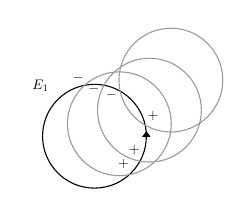
\begin{tikzpicture}[x=0.75pt,y=0.75pt,yscale=-1,xscale=1]
%uncomment if require: \path (0,95); %set diagram left start at 0, and has height of 95

%Shape: Circle [id:dp37777408295388804] 
\draw   (21,59.5) .. controls (21,45.69) and (32.19,34.5) .. (46,34.5) .. controls (59.81,34.5) and (71,45.69) .. (71,59.5) .. controls (71,73.31) and (59.81,84.5) .. (46,84.5) .. controls (32.19,84.5) and (21,73.31) .. (21,59.5) -- cycle ;
%Shape: Circle [id:dp4562198988843913] 
\draw  [color={rgb, 255:red, 155; green, 155; blue, 155 }  ,draw opacity=1 ] (47.5,46.94) .. controls (47.5,33.14) and (58.69,21.94) .. (72.5,21.94) .. controls (86.31,21.94) and (97.5,33.14) .. (97.5,46.94) .. controls (97.5,60.75) and (86.31,71.94) .. (72.5,71.94) .. controls (58.69,71.94) and (47.5,60.75) .. (47.5,46.94) -- cycle ;
%Shape: Circle [id:dp8913971633985722] 
\draw  [color={rgb, 255:red, 155; green, 155; blue, 155 }  ,draw opacity=1 ] (33,53.5) .. controls (33,39.69) and (44.19,28.5) .. (58,28.5) .. controls (71.81,28.5) and (83,39.69) .. (83,53.5) .. controls (83,67.31) and (71.81,78.5) .. (58,78.5) .. controls (44.19,78.5) and (33,67.31) .. (33,53.5) -- cycle ;
%Shape: Circle [id:dp05970043129919356] 
\draw  [color={rgb, 255:red, 155; green, 155; blue, 155 }  ,draw opacity=1 ] (57.81,32.47) .. controls (57.81,18.66) and (69,7.47) .. (82.81,7.47) .. controls (96.62,7.47) and (107.81,18.66) .. (107.81,32.47) .. controls (107.81,46.27) and (96.62,57.47) .. (82.81,57.47) .. controls (69,57.47) and (57.81,46.27) .. (57.81,32.47) -- cycle ;
%Straight Lines [id:da04725899028195979] 
%\draw[densely dotted]  (21,59.5) -- (71,59.5) ;


%Flowchart: Extract [id:dp5267407418119328] 
\draw  [fill={rgb, 255:red, 0; green, 0; blue, 0 }  ,fill opacity=1 ] (71,57.45) -- (72.52,59.55) -- (69.48,59.55) -- cycle ;

\draw (60,73) node [scale=0.5]  {$+$};
% Text Node
\draw (65.22,66) node [scale=0.5]  {$+$};
% Text Node
\draw (74.22,50) node [scale=0.5]  {$+$};
% Text Node
\draw (54.22,39.56) node [scale=0.5]  {$-$};
% Text Node
\draw (45.62,36.96) node [scale=0.5]  {$-$};
% Text Node
\draw (38.02,31.56) node [scale=0.5]  {$-$};


% Text Node
\draw (20,35) node [scale=0.5]  {$E_{1}$};
\end{tikzpicture}

\begin{tikzpicture}

\matrix [matrix of nodes,row sep=,row sep=0mm,
column 1/.style={nodes={rectangle,draw,minimum width=1.5em, minimum height=0.5em}},
column 2/.style={nodes={rectangle,draw,minimum width=1.5em, minimum height=0.5em}},
column 3/.style={nodes={rectangle,draw,minimum width=1.5em, minimum height=0.5em}},
column 4/.style={nodes={rectangle,draw,minimum width=1.5em, minimum height=0.5em}},
column 5/.style={nodes={rectangle,draw,minimum width=1.5em, minimum height=0.5em}},
column 6/.style={nodes={rectangle,draw,minimum width=1.5em, minimum height=0.5em}},
column 7/.style={nodes={rectangle,draw,minimum width=1.5em, color=gray, minimum height=0.5em}},
column 8/.style={nodes={rectangle,draw,minimum width=1.5em, color=gray, minimum height=0.5em}},
column 9/.style={nodes={rectangle,draw,minimum width=1.5em, color=gray, minimum height=0.5em}},
column 10/.style={nodes={rectangle,draw,minimum width=1.5em, color=gray, minimum height=0.5em}},
column 11/.style={nodes={rectangle,draw,minimum width=1.5em, color=gray, minimum height=0.5em}},
column 12/.style={nodes={rectangle,draw,minimum width=1.5em, color=gray, minimum height=0.5em}}
] (O)
{
$+$ & $-$ & $-$ & $-$ & $+$ & $+$ & $+$ & $-$ & $-$ & $-$ & $+$ & $+$\\
%$+$ & $-$ & $-$ & $-$ & $+$ & $+$\\
};

\node at (-4,-0.5) {$0$};
\node at (0,-0.5) {$2\pi$};
\end{tikzpicture}
    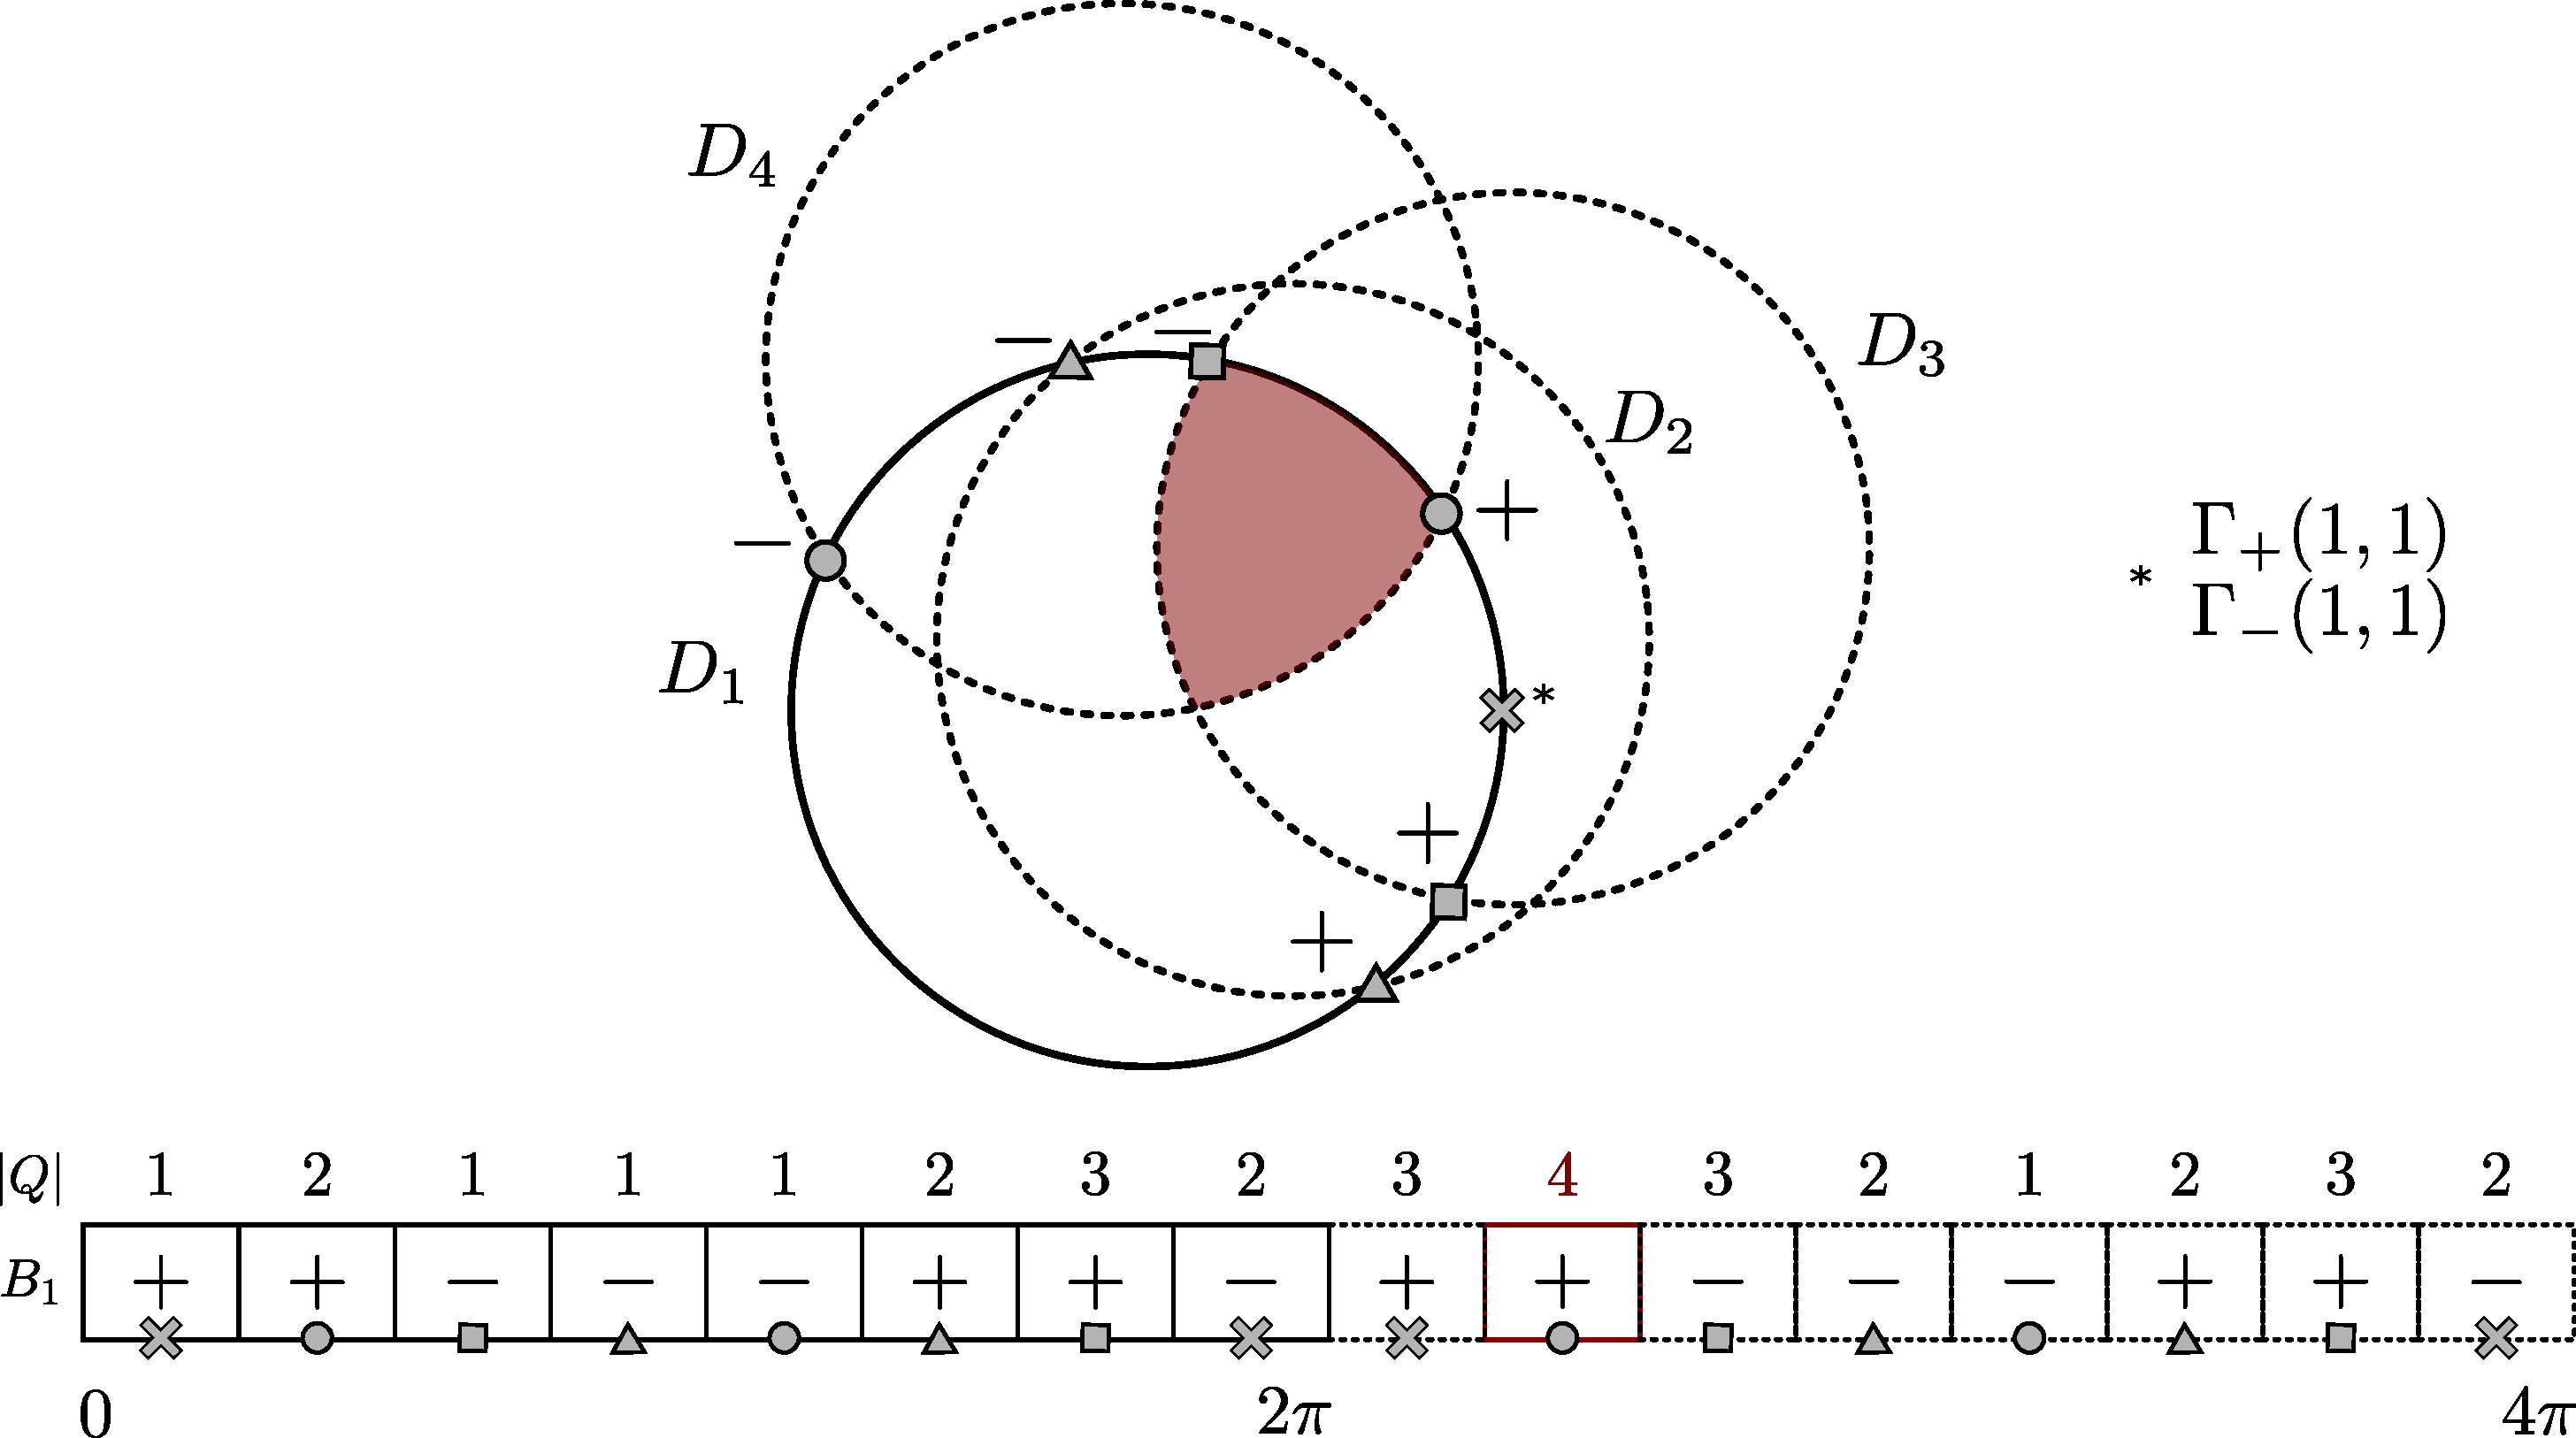
\includegraphics[scale=.28]{tex/figures/3_disks_intersect2.pdf}
    \fautor
    \label{fig:array_disks}
\end{figure}

\begin{teorema}\label{lema:disk}
	\autoref{algoritmo:mcd_1} for solving the Maximum Clique Problem has a $\bigO((n+K)\log{n})$ run time complexity, where $K$ is the number of intersections of the $n$ disks.
\end{teorema}

\begin{proof}
	Finding every intersection can be done in $\bigO((n+K)\log{n})$  by a plane sweep, the method is described in \citeonline{bentley:1979}. 
	Because sorting the intersection angles needs to be done, an additional $\bigO(K\log{K})$ pre-processing is added. All the other operations can be done in constant time. Therefore, the final algorithm complexity is $\bigO((n+K)\log{n})$.
\end{proof}

If a simpler implementation is desired, or the number of intersections is large, determining the set $I_i$ (the set of disks that intersect with $D_i$, defined in \autoref{algoritmo:mcd_1}) can be simply done in $\bigO(n^2)$, making the algorithm have a worst-case complexity of $\bigO(n^2\log{n})$.

\begin{algoritmo}[b]
\caption{Algorithm for MCD-1.}\label{algoritmo:mcd_1}
\begin{algorithmic}[1]
\Require{A set of points $\Pp=\{p_1,\dots,p_n\}$ with weights $\Ww=\{w_1, \dots, w_n\}$.}
\Ensure{The maximum cover by a unit disk.}

\item[]

\Procedure{$MCD_1$}{$\Pp$}
\State $Q_{best} \gets \{\}$
\State $ans \gets$ center of $D_1$
\ForAll{$p_i \in \Pp$}
\State Let $D_i$ be the disk with center at $p_i$
\State Let $B_i$ be the list of intersection angles of $D_i$ as defined by \autoref{eq:b_i}.

\State $Q \gets \{\}$ \Comment{The set of active disks.}
\For{$a \in B_i$}\Comment{Assuming $B_i$ is sorted.}
\State Let $D_a$ be the disk that intersects $D_i$ at angle $a$. 
\If{$a$ is a starting angle}
\State $Q \gets Q \cup \{D_a\}$
\Else
\State $Q \gets Q \setminus \{D_a\}$
\EndIf
\If{$w(Q_{best}) < w(Q)$} \Comment{$w(Q)$ returns the weights of the disks in $Q$.}
\State $Q_{best} \gets Q$
\State $ans \gets $ point corresponding to the intersection angle $a$
\EndIf

\EndFor
\EndFor

\State \Return $ans$
\EndProcedure
\end{algorithmic}
\end{algoritmo}

\section{An algorithm for MCD}

A simple adaptation can be done on \autoref{algoritmo:mcd_1} to make it return a CLS that contains an optimal solution of MCD for that disk. This is shown in \autoref{algoritmo:mcd_cls}. 
Notice also that MCD-1 is defined only for unit disks, however, this constrained can be dropped, as it is introduced just for the sake of keeping the text more simple and \autoref{algoritmo:mcd_1} works for any radius. A result about the runtime complexity of \autoref{algoritmo:mcd_cls} has already been given by \autoref{lema:disk}, the following result states about the adaption of it to be used in an algorithm for MCD.

\begin{lema}\label{lema:mcd}
	Suppose that an instance of MCD and an index $j\in\{1, \dots, m\}$ are given.
	Then \autoref{algoritmo:mcd_cls}, when given the instance $(\Pp, \Ww, r_j)$ as input, returns a CLS $S_j$ of size $\bigO(n^2)$, such that $q^*_j\in S_j$, with $(q^*_1, \dots, q^*_m)$ being an optimal solution of the given MCD's instance.
\end{lema}

\begin{proof}
It can be seen that in any solution of MCD, a disk placed at a point $q$ that covers at least one point $p \in \Pp$ has a correspondence to the Maximum Weight Clique Problem: the point $q$ is inside an intersection area of at least one disk and that area is bounded by some disk, which means it will be checked by \autoref{algoritmo:mcd_cls} as a candidate to be an optimal solution. The number of points \autoref{algoritmo:mcd_cls} goes through is $\bigO(n^2)$, then
obviously $|S_j|=\bigO(n^2)$.
\end{proof}

Then, with \autoref{algoritmo:mcd_cls}, an algorithm for MCD that checks every possible center for every disk yields a $\bigO(n^{2m})$ run-time complexity.
This algorithm is described in \autoref{chapter:ellipses} for the axis-parallel ellipses case.

It is worth mentioning that the choice of developing a different method for the problem, instead of using the one from \citeonline{cabello:2006}, is taken for the sake of simplicity, considering both algorithms achieve similar bounds.

\begin{algoritmo}
	\caption{Algorithm for MCD-1 that returns a CLS.}\label{algoritmo:mcd_cls}
	\begin{algorithmic}[1]
		\Require{A set of points $\Pp=\{p_1,\dots,p_n\}$ with weights $\Ww=\{w_1, \dots, w_n\}$, and a radius $r\in\R_{>0}$.}
		\Ensure{A CLS for the disk given by radius $r$.}
		
		\item[]
		
		\Procedure{$MCD_1$}{$\Pp, \Ww, r$}
		\State $S \gets \{\}$
		\ForAll{$p_i \in \Pp$}
		\State Let $D_i$ be the disk with center at $p_i$
		\State Let $B_i$ be the list of intersection angles of $D_i$ as defined by \autoref{eq:b_i}.
		
		\State $Cov \gets \{\}$
		\For{$a \in B_i$}\Comment{Assuming $B_i$ is sorted.}
		\State Let $q_a$ be the intersection point correspondent to angle $a$. 
		\State $S \gets S \cup \{q_a\}$	
		\EndFor
		\EndFor
		
		\State \Return $S$
		\EndProcedure
	\end{algorithmic}
\end{algoritmo}

\chapter{Maximum Covering by Ellipses}
\label{chapter:mce}
Similarly to the method developed in \cite{church:1984} for the Euclidean PMCLP, we will describe a Candidate List Set (CLS) of possible locations for each ellipse and then propose an algorithm that constructs solutions combining the possible locations in each ellipse's CLS.
Also, based on the approach of \cite{church:1984} for the Euclidean PMCLP, and in \cite{chazelle:1986} for the problem of covering points by one unit disk, we will construct the CLS for each ellipse by using a property of the one-facility MCE.
Although, it is intuitive that it is possible to adapt the ideas used for solving the problems involving Euclidean disks for axis-parallel ellipses, using the results of \cite{bi}, which studies the problem of determining the intersection of $n$ strictly convex disks with fixed radius, we will prove that for MCE, we have all the necessary geometric properties to develop an algorithm following those approaches.

We start by introducing a lemma stating that any solution of the one-facility MCE can be related to the intersection of coverage regions of ellipses centered at the points covered in that solution. 

\begin{lem}\label{lema:mce-mwc}
	Let $(\Pp, \Ww, \{(a, b)\})$ be an instance of MCE, and $q\in \R^2$. If $\Pp \cap E(q) = A$, then $q \in \cap_{p\in A} E(p)$.
\end{lem}
\begin{proof}
	Let $u, v \in \R^2$, then we have that $u \in E(v)$ if, and only if $v \in E(u)$, which is proved simply by observing that:
	\begin{equation}\label{eq:peq}
	u \in E(v) \Leftrightarrow ||u-v||_{a, b, 0} \le 1 \Leftrightarrow v \in E(u).
	\end{equation}
	As $\Pp \cap E(q) = A$ can be written as: for all $p \in A$, $p \in E(q)$. Then, using \autoref{eq:peq}, we get that for all $p \in A$, $q \in E(p)$, which implies that $q \in \cap_{p\in A} E(p)$.
\end{proof}



%To define this equivalent problem, we need to first state an ellipse's property.
%Let $(\Pp, \Ww, \{(a, b)\})$ be an instance of MCE with one facility, and  $p, q \in \R^2$, we have that

%The equivalent problem is given by $n$ ellipses with shape parameters $(a, b)$ centered at $\Pp$. Let $q\in\R^2$ be a solution of MCE for one facility, by applying \autoref{eq:peq} to every point covered by $E(q)$, we obtain that
%\begin{equation}\label{eq:mce-mwc}
%\Pp \cap E(q) = \{p_i\in\Pp \colon q\in E(p_i)\},
%\end{equation}
%which implies that the problem of determining $q\in\R^2$ to maximize $w(\{p_i\in\Pp \colon q\in E(p_i)\})$, is equivalent to MCE for one facility. This changes the problem from determining a location for an ellipse given $n$ points to the problem of finding a point given $n$ ellipses with fixed locations.

%Let $A\subset \Pp$, from \autoref{eq:mce-mwc}, we have that if $\Pp \cap E(q) = A$ then $q \in \cap_{p\in A} E(p)$. 

From , if we could identify every 

Let $A \subset \Pp$, $|A|>1$, let us consider the intersection region $\cap_{p\in A} E(p) \neq \emptyset$. From \autoref{lema:mce-mwc}, we can also conclude that if $q \in \cap_{p\in A} E(p)$, then $A \subset \Pp \cap E(q)$.


In \cite{church:1984}, for the Euclidean PMCLP, it was proved that the border of this region contains at least one point that is an intersection between two fixed-radius circles with centers in $A$. This, as it turns out, is also true for ellipses, and a proof can be obtained from \cite{bi} where the problem of determining the intersection region of $n$ fixed-radius disks in a strictly convex normed plane is studied.
From that, we can conclude that there exists $u, v \in A$ and $q \in \partial E(u) \cap \partial E(v)$, such that $q \in \cap_{p\in A} E(p)$.
Before defining the CLS for each ellipse, we introduce a lemma stating two basic, and yet important properties about the intersection between two axis-parallel ellipses that have the same shape and distinct locations.

\begin{lem}\label{lema:e2p}
	Let $E$ be the coverage region of an axis-parallel ellipse with shape parameters $(a,b)$; and $v \in \R^2$, $v\neq0$. Then $|\partial E(0) \cap \partial E(v)| \le 2$, and $\partial E(0) \cap \partial E(v)$ can be determined analytically.
\end{lem}

\begin{proof}
	To determine the intersection points, consider the equality between the equations of $\partial E(0)$ and $\partial E(v)$:
	$x^2/a^2 + y^2/b^2 = (x-v_x)^2/a^2 + (y-v_y)^2/b^2.$
	This expression can be reduced to $y=\alpha x + \beta$, for some $\alpha, \beta$, which can then be plugged into $\partial E(0)$'s equation obtaining $x^2/a^2 + (\alpha x + \beta)^2/b^2 = 1$.
	We obtain the intersection points by solving this quadratic equation for $x$, and then, for each value of $x$,  determining $y$ from $y=\alpha x + \beta$.
\end{proof}
Next, we define the CLS of each ellipse, considering also the case where, in an optimal solution, an ellipse covers only one point.
\begin{definition}\label{def:cls_mce}
	Given an instance of MCE, for all $k \in \{1, \dots, m\}$, we define the CLS for the $k$-th ellipse as
	\begin{equation}
	S_k = \Pp \cup \left(\bigcup_{1 \le i < j \le n} \partial E_k(p_i) \cap \partial E_k(p_j) \right).
	\end{equation}
\end{definition}

By \autoref{lema:e2p}, the CLS for each ellipse can be computed in $\bigO(n^2)$, and $|S_k| \le n + 2\binom{n}{2}$. Next, we establish a lemma stating that the set of solutions obtained by combining the possible locations in each ellipse's CLS contains at least one optimal solution.

\begin{thm}\label{thm:mce}
	Given an instance of MCE, and $S_1, \dots, S_m$ as defined by \autoref{def:cls_mce}, then the set $\Omega = \{(q_1, \dots, q_m) \colon \textnormal{ for all }q_k \in S_k \}$ contains an optimal solution of MCE and $|\Omega| \le n^{2m}$. 
\end{thm}
\begin{proof}
	Let $Q^*$ be an optimal solution of MCE for the given instance. Then, we are going to prove that there exists $Q' \in \Omega$, which is also optimal.
	
	For each $k=1, \dots, m$, let $X_k = \{p_i \in \Pp\colon p_i \in E_k(q_k^*)\}$.
	
	%If $|X_k| = 0$, then any $q_k \in S_k$ makes $X_k \subset \Pp \cap E_k(q_k)$.
	
	If $|X_k| \le 1$, then there is at least one element in $S_k$ that makes $X_k \subset \Pp \cap E_k(q_k)$.
	
	If $|X_k| > 1$, then let $Y_k = \cap_{p \in X_k}E_k(p)$. By the results of \cite{bi}, we have that the boundary of $Y_k$ has vertices in the pairwise intersections of $\{\partial E_k(p) \colon p \in X_k\}$. Therefore, at least one vertex of $Y_k$ is in $S_k$, and any of those vertices produce a solution that covers at least the same points covered by $Q^*$.
	
	Lastly, we have that $|S_k| \le 2\binom{n}{2} + n = n(n+1)/2 \le n^2$. Hence, $|\Omega| \le n^{2m}$.
\end{proof}

With all this in hand, we define \autoref{algoritmo:mce}, which goes through every possible combination in the CLS of each ellipse. As evaluating each solution can be done in $\bigO(nm)$, we have that \autoref{algoritmo:mce} has $\bigO(mn^{2m+1})$ runtime complexity. 
In \autoref{section:numerical}, we give more details about the implementation of \autoref{algoritmo:mce} and analyze some numerical experiments for instances proposed in \cite{canbolat, andreta}, and for some new ones.

\begin{algorithm}
	\caption{Algorithm for MCE}\label{algoritmo:mce}
	
	\begin{algorithmic}[1]
		\Require{A set of points $\Pp=\{p_1,\dots,p_n\}$, a list of weights $\Ww=\{w_1, \dots, w_n\}$, and a list of shape parameters $\Rr=\{(a_1, b_1), \dots, (a_m, b_m)\}$.}
		
		\Ensure{An optimal solution for MCE.}
		
		\item[]
		\Procedure{$MCE$}{$\Pp, \Ww, \Rr$}
		\State \Return $MCE_{bt}(\Pp, \Ww, \Rr, 1)$
		\EndProcedure
		\State
		\Procedure{$MCE_{bt}$}{$Z, \Ww, \Rr, j$}
		\If{$j = |\Rr|+1$}
		\State \Return $0$
		\EndIf
		
		\State $(q_j^*, \dots, q_m^*) \gets (0, \dots, 0)$
		\State Let $S_j$ be the CLS for the $j$-th ellipse as defined by \autoref{def:cls_mce}.
		%\State $S_j \gets \textnormal{CLS-MCE}(Z, a_j, b_j)$
		\For{$q_j \in S_j$}
		\State $Cov \gets \Pp \cap E_j(q_j)$
		\State $(q_{j+1}, \dots, q_m) \gets MCE_{bt}(Z \setminus Cov, \Ww, \Rr, j+1)\}$
		
		\If{$w(\cup_{k=j}^m Z \cap E_k(q_k)) >  w(\cup_{k=j}^m Z \cap E_k(q_k^*))$}
		\State $(q_j^*, \dots, q_m^*) \gets(q_j, \dots, q_m)$
		\EndIf
		\EndFor
		
		\State \Return $(q_j^*, \dots, q_m^*)$
		\EndProcedure
	\end{algorithmic}
\end{algorithm}

%\chapter{Every Center and Angle of Rotation of an ellipse given its shape and three points}
\chapter{Determining every location of an ellipse given its shape and three points}
\label{chapter:e3p}
The problem of finding every center and angle of rotation of a fixed shape ellipse which makes it have three points on its border is presented in this section. Even though its simple statement--it is short and uses only basic mathematical concepts--we were not able to find any work on it, or even on related problems. 
As a result, starting from scratch, we ended up trying a handful of approaches with most of them failing on the way. We try to give a review of some of those, and also make a case for the method we propose in terms of velocity of convergence and quality of the solutions that it finds.

We refer to this problem as \sigla{E3PNT}{Ellipse by Three points}, and an instance of it is given by three points $u, v, w \in \R^2$ and $E$, an ellipse with shape parameters $(a, b) \in \R^2_{>0}$, with $a > b$. A solution of E3PNT is a pair $(q, \theta) \in \R^2\times[0, \pi]$, such that $\{u, v, w\} \subset \tilde{E}(q, \theta)$. In other words, the goal is to develop a method to find every solution of E3PNT. 


\section{Transforming the problem}

To make it simpler, let us translate the system, so the point $u$ is at $(0,0)$. Then, we assume that the ellipse is actually axis-parallel and the points are the ones rotating. When an angle is found such that the three points lie on the border of the axis-parallel ellipse, a linear transformation can be applied to compress the x-axis by $\frac{b}{a}$, transforming the ellipse into a circle of radius $b$. This transformation can be seen on \autoref{fig:circumscribed-circle} where a solution of the E3PNT is transformed into a solution of the problem of finding a circumscribed circle of a triangle. 
This process can be parametrized by the angle of rotation of the points, as described by \autoref{eq:trpnts}, and because of the invertibility of linear transformations solutions for E3PNT can be obtained by reversing the transformations.

\begin{figure}
	\centering
	\caption{Transforming an ellipse into a circle. T1, T2, and T3 represent the steps of the transformation.}
	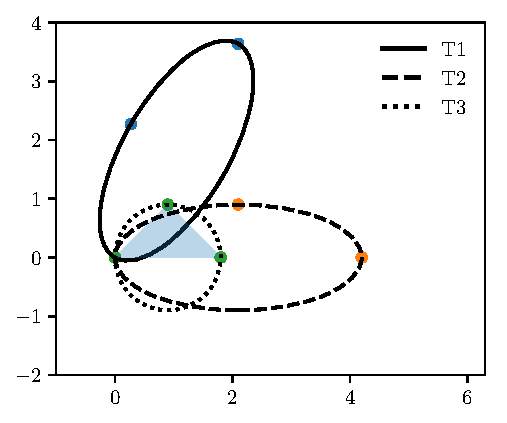
\includegraphics{tex/figures/scripts/circumscribed-circle}
	\fautor
	\label{fig:circumscribed-circle}
\end{figure}
\begin{equation}\label{eq:trpnts}
\varphi(p, \theta)=\left[\begin{array}{cc}
\frac{b}{a}&0\\
0&1
\end{array}\right]
\left[\begin{array}{cc}
\cos{\theta}&\sin{\theta}\\
-\sin{\theta}&\cos{\theta}
\end{array}\right]\left[\begin{array}{c}
p_x\\
p_y
\end{array}\right].
\end{equation}

Then, the problem to be solved is finding a circumscribed circle of the triangle formed by the points $(0, 0), \varphi(v, \theta)$ and $\varphi(w, \theta)$, such that the circle has radius $b$. As, for three non-colinear fixed points, there is always an unique circumscribed circle for the triangle formed by those three points, the only variable to be determined ends up being the angle of rotation $\theta$.

Let $A(\theta)$ be the area of the triangle formed by the points $(0, 0), \varphi(v, \theta)$ and $\varphi(w, \theta)$--note that the transformation does not preserve distance or area. Then, the radius $R$ of the circumscribed circle is given by \autoref{eq:circumscribed_circle} \cite[p.~189]{johnson1960}.

\begin{equation}\label{eq:circumscribed_circle}
R = \dfrac{\norm{\varphi(v, \theta)}\norm{\varphi(w, \theta)}\norm{\varphi(v, \theta)-\varphi(w, \theta)}   }{4A(\theta)}.
\end{equation}

Imposing the radius to be equal $b$ and squaring to eliminate the square roots present in the Euclidean distance, a function $\xi : [0, \pi) \mapsto \mathbb{R}_{>0}$ is defined by \autoref{eq:circumscribed_circle_b} in such a way that its zeros determine solutions to the E3PNT's instance. Two questions about $\xi(\theta)$ that arise are: is its set of roots finite? And, can they be found analytically?

\begin{equation}\label{eq:circumscribed_circle_b}
\xi(\theta) = 16b^2A(\theta)^2 - \norm{\varphi(v, \theta)}^2\norm{\varphi(w, \theta)}^2\norm{\varphi(v, \theta)-\varphi(w, \theta)}^2.
\end{equation}

\subsection{The number of solutions is limited}

The method developed on \autoref{chapter:ellipses_n} iterates over every solution of E3PNT for every triplet of points, this is only possible if the size of this set of solutions is limited. Also, if this was not true, it would be very difficult to describe a method to get every solution which could be infinite.

It turns out that $\xi$ can be written as a real trigonometric polynomial of degree $6$ in the format given by \autoref{eq:trig_poly_2}, which implies that it can have up to $12$ distinct roots.
 To show that, just note that it is possible to write $\norm{\varphi(v, \theta)}^2$ and $A(\theta)^2$ in that form, as it can be seen on \autoref{eq:dd} and \autoref{eq:dd2}. It is also possible to see that the term of higher the degree of $\xi$ is the multiplication of the three squared distances. As $\norm{\varphi(v, \theta)}^2$ has degree $2$, the degree of $\xi$ is $6$.
\begin{align}\label{eq:dd}
	\norm{\varphi(v, \theta)}^2 = (v_x\frac{b}{a}\cos\theta + v_y\frac{b}{a}\sin\theta)^2 + (v_y\cos\theta - v_x\sin\theta)^2\\
	\label{eq:dd2} A(\theta)^2=\dfrac{1}{4}\det\left(
	\begin{array}{cc}
		v_x\frac{b}{a}\cos\theta + v_y\frac{b}{a}\sin\theta&v_y\cos\theta - v_x\sin\theta\\
		w_x\frac{b}{a}\cos\theta + w_y\frac{b}{a}\sin\theta&w_y\cos\theta - w_x\sin\theta
	\end{array}\right)^2
\end{align}

Because ellipses are symmetrical with respect to their major-axis, and any rotation in the interval $[0, \pi)$ is identical to a rotation in $[\pi, 2\pi)$, the number of different solutions is cut in half.
Therefore, the number of angles of rotation and centers that an ellipse of fixed shape can be placed, so it has three fixed points on its border is limited to $6$.

\section{An attempt using the conic general equation}

The idea of this approach was to use the six-parameter conic equation to represent an ellipse. This equation is given by \autoref{eq:gen_ellipse}.

\begin{equation}\label{eq:gen_ellipse}
Ax^2+Bxy+Cy^2+Dy+Ex+F=0.
\end{equation}
This equation actually represents any conic, for it to be an ellipse the condition $B^2 -4AC < 0$ must be satisfied.

Setting the first point to be the origin, we get $F=0$, using the other two points, it is possible to write $D$ and $E$ in terms of $A, B, C$. As any multiple of \autoref{eq:gen_ellipse} represents the same conic, we can set $B$ to be equal $1$. Then, we end up with two variables, $A$ and $C$, and still need to impose that the final equation represents an ellipse and its major-axis and minor-axis have the predefined value. Let $\Delta=4AC-B^2=4AC-1$, \autoref{eq:gen_ellipse_a} and \autoref{eq:gen_ellipse_b} for both major-axis and minor-axis respectively, assuming $F=0$.

\begin{align}\label{eq:gen_ellipse_a}
a^2 = \dfrac{2\dfrac{AE^2 -BDE +CD^2}{\Delta}}{A + C - \sqrt{1 + (A-C)^2}}\\
\label{eq:gen_ellipse_b}b^2 = \frac{2\dfrac{AE^2 -BDE +CD^2}{\Delta}}{A + C + \sqrt{1 + (A-C)^2}}
\end{align}

These two equations define two curves in $\R^2$ with $A$ and $C$ being the chosen variables. The solutions lie in the set of intersection of these curves. Finding this set was judged to be non-trivial and probably could be approximated numerically, however, we decided not to further pursue this approach.

Another idea which has been explored was working with the ratio $\frac{a^2}{b^2}$ which becomes an expression that allows $A$ to be written as a function of $C$. This function appeared, at first we thought, to be monotonic, we tried to develop a method based on that, however, cases where the function does not behave as nicely were found. It is likely that developing a method to approximate solutions working with this function is possible, but we decided not to continue on this track.


\section{An approximation method}

One of the most useful techniques when dealing with complicated functions is approximation. They appear in various methods whenever a derivative or integral needs to be calculated or for example, in our case, when the roots of a function need to be determined. In general, one has a function $f$ that is part of a family of functions $\mathcal{A}$ and wants to select a simpler function $f^*$ from a set of functions $\mathcal{A^*}$, such that $f^*$ is close enough to $f$ \cite[p.~3]{powell}. For this problem, the approximation of $\xi(\theta)$ on the interval $[0, \pi)$ is considered. The approximation set of functions is going to be the set of $n$-degree Chebyshev polynomials which the roots can be found through determining the eigenvalues of a $n$ by $n$ matrix.


\subsection{Chebyshev interpolation}

Chebyshev polynomials are widely used in Numerical Analysis in areas like numerical integration, polynomial approximation, and ordinary and partial differential equations.
They are also very useful in practice and are present in extension libraries in Python and MATLAB.

Because of the scope of this work, only a brief introduction of Chebyshev polynomials of the first kind and its usage in polynomial interpolation is given. For a more thorough work on the subject, please check the book by \citeonline{chebbook}.

We refer to $T_n : [-1, 1] \mapsto [-1, 1]$ as the $n$-degree Chebyshev polynomial of the first kind, and it is defined as follows:

\begin{equation}
T_n(x) = \cos({n\arccos x})
\end{equation}

It is important to mention that this definition can be extended to the whole real line. Using some trigonometric identities, $T_n$ can also be expressed as a recurrence relation:

\begin{equation}
T_n(x) = 2xT_{n-1}(x) - T_{n-2}(x).
\end{equation}

An important property worth bringing up is that Chebyshev polynomials are orthogonal and form a basis for the polynomial space. This implies that any $p_n$ of degree up to $n$ can be expressed as a truncated Chebyshev series:

\begin{equation}\label{eq:chebseries}
p_n(x) = \sum_{j=0}^{n} a_j T_j(x).
\end{equation}

One of the greatest qualities of Chebyshev polynomials is its numerical stability. \citeonline{gautschi:1979} showed that the matrix that maps polynomials onto its coefficients written in the power form\footnote{A polynomial is in the power form or the monomial form if it can be written as $\sum_{j=0}^{n}a_jx^j$} has a condition number that grows exponentially with $n$. On the other hand, the matrix that converts polynomials to the Chebyshev basis as \autoref{eq:chebseries}, has a linear condition number bounded by $\sqrt{2}n$.

Polynomial interpolation is a form of approximating a function by a polynomial of degree $n$ that passes through $n+1$ chosen points. In fact, this polynomial is unique and it is determined by Lagrange's formula:

\begin{equation}\label{eq:lagrange}
f_n(x) = \sum_{j=0}^{n} f(x_j)\dfrac{\prod_{k \neq j}^{n+1} (x-x_k)}{\prod_{k \neq j}^{n+1} (x_j-x_k)},
\end{equation} 
with $f$ being the function to be approximated, and $f_n$ the unique $n$-degree polynomial that passes through $\{(x_j, f(x_j)): j=0, 1, \dots n\}$. Because of the uniqueness of interpolant polynomials, there is a direct link between the quality of an approximation and the points chosen to interpolate. As a matter of fact, depending on the points one chooses, even increasing the degree of the interpolation makes the approximation worsen. This is known as Runge's phenomenon and an example can be seen in \citeonline[p.~37]{powell} where uniformly spaced points are chosen to interpolate the function $f(x) = (1+x^2)^{-1}$ on the interval $[-5, 5]$. 

That is where Chebyshev interpolation comes in. Instead of choosing $n+1$ arbitrary points, the $n+1$ roots of $T_{n+1}$, which are also known as Chebyshev Nodes, are chosen as the interpolation points:
\begin{equation}
x_j = \cos{\left(\dfrac{\pi(k-\frac{1}{2})}{n+1}\right)},
\end{equation}
for $j=1, \dots, n+1$. This particular choice defeats Runge's phenomenon and provides a convergent approximation. 

Note that, if the domain of the function to be interpolated is defined on a range other than $[-1, 1]$, let us say $[a, b]$, then a transformation can be done to map it to the Chebyshev Nodes' domain:
\begin{equation}
\hat{x_j} = \frac{a+b}{2} + \frac{b-a}{2}x_j.
\end{equation}

Then, the Chebyshev interpolation of a function $f: [a, b] \mapsto \R$ can be determined using Lagrange's formula and the points $\hat{x}_1, \dots, \hat{x}_n$. 
As it was mentioned, finding the roots of a polynomial written in the monomial form can be done by determining the eigenvalues of a so-called Frobenius companion matrix. For small $n$ this works fine, however, converting the polynomial obtained by \autoref{eq:lagrange} to the power form, as $n$ grows, becomes a very ill-conditioned problem. 
An alternative method can be found in \citeonline{boyd:2013} where the Chebyshev interpolation is calculated directly as a truncated Chebyshev series, as in \autoref{eq:chebseries}, in $\bigO(n^2)$. Also, given a polynomial written in the Chebyshev basis, a $n\times n$ matrix can be constructed, such that its eigenvalues are the roots of that polynomial. \citeonline{boyd:2013} refers to this matrix as the Chebyshev-Frobenius companion matrix.

Therefore, the whole process of interpolating and finding the roots can be done using only Chebyshev polynomials, which have great numerical stability. Also, Chebyshev-Frobenius matrices have the same property as companion matrices which allows their eigenvalues to be found by a QR decomposition. Summing the two steps, a $\bigO(n^2)$ algorithm can be achieved.

The last question that needs to be addressed is how close the roots of the Chebyshev interpolant $f_n$ are to the roots of $\xi$?

Even though $\xi$ is complicated enough, in a sense that finding its roots directly is no trivial task, it is a very well-behaved function: it is analytic and  has infinitely many continuous and integrable derivatives. This satisfy all the requirements of the result in \citeonline[p.~28]{gottlieb} which says that if a function has $m$ continuous and integrable derivatives on a closed interval, then its absolute difference between the Chebyshev truncate series is $\bigO(n^{-m})$. Also, in \citeonline{battles:2004} a theorem is presented stating that if a function is analytic on a neighborhood of $[-1, 1]$, then the convergence is $\bigO(C^n)$, for some $C<1$.

To choose the degree of the interpolation we use the last coefficient rule-of-thumb introduced by \citeonline[p.~50]{boyd:2001}. There is no guarantee that this method will choose $n$, such that $f_n$ is close enough to $\xi$ everywhere on $[0, \pi)$, nonetheless, in practice, it is taken to be a good estimate for the error $r_n$:
\begin{equation}
r_n = \max_{0 \le \theta \le \pi} |f_n(\theta) - \xi(\theta)|.
\end{equation}


\section{Converting $\xi$ into a polynomial}

On \autoref{chapter:definitions} a brief introduction is given on how to get the roots of a polynomial. For that reason, we discuss two ways of converting $\xi$ into a polynomial in this section. Symbolic computing was used to compute the polynomials, in practice an external Python library called SymPy was utilized (see \citeonline{sympy} for more details).

The first attempt was using the identity $x = \tan{\frac{\theta}{2}}$ from which it is possible to construct a $12$-degree polynomial. At first,  the root-finding algorithm described on \autoref{chapter:definitions} seemed to work fine and return every solution of E3PNT, however, we later found out that for some instances, priorly known roots were not being found. The cause was not for sure identified, but a good guess would be that for angles which are greater than $\frac{\pi}{4}$, $x$ starts growing too rapidly which could lead to numerical instability.

The second approach is based on a idea published on \citeonline{boyd:2006} which uses the identities on \autoref{eq:complex_trig} to convert real trigonometric polynomials into univariate complex polynomials in order to obtain its roots using the companion matrix scheme.
Also, in \citeonline{weidner} it is said that computing the roots of a real trigonometric polynomial through this transformation does not yield loss of accuracy.

\begin{align}\label{eq:complex_trig}
\cos{\theta} = \dfrac{e^{i\theta} + e^{-i\theta}}{2}\\
\sin{\theta} = \dfrac{e^{i\theta} - e^{-i\theta}}{2i}.
\end{align}

It is possible to show that with that substitution and changing the variable to $z=e^{i\theta}$, we obtain the following function $g : \mathbb{S} \mapsto \mathbb{C}$, with $\mathbb{S}$ being the unit circle ($\mathbb{S} = \{z \in \mathbb{C} : |z|=1\}$):

\begin{equation}
g(z)=\sum_{k=0}^{12} c_k z^{k-6},
\end{equation}
for some $c_0, \dots, c_{12} \in \mathbb{C}$. Even though $g$ is not a polynomial, it is easy to obtain one from it. Firstly, the negative exponentials need to be shifted, this can be done by just multiplying $g$ by $z^6$. Secondly, the domain cannot be restricted to the unit circle, so we define $h : \mathbb{C} \mapsto \mathbb{C}$ as:
\begin{equation}
h(z) = z^6 g(z) = \sum_{k=0}^{12} c_k z^k.
\end{equation}

Then, by its definition is possible to see that every root of $g$ is also a root of $h$. Conversely, every root $\hat{z}$ of $h$ which is in $\mathbb{S}$--or $|\hat{z}|=1$--is also a root of $g$. Naturally, the angle of a root $\hat{z}$ of $g$ is a root of $\xi$ by Euler's Formula.

It is possible to make another reduction to obtain a degree-$6$ polynomial from $h$ whose roots form a superset of the roots of $g$. As it has been mentioned on this chapter, an ellipse is symmetric with respect to its own axis. This means $\theta$ and $\pi + \theta$ are equivalent angles of rotation for any ellipse, thus $\xi(\theta) = \xi(\pi + \theta)$\footnote{$\xi$ is only defined over $[0, \pi)$, so this equality is not actually valid.}. 
On \autoref{chapter:definitions}, it was stated that the angle of $z$ and $-z$ has the same symmetry with each other as an ellipse's angle of rotation:
\begin{equation*}
angle(-z) = \pi + angle(z).
\end{equation*}
From that, as $g(e^{i\theta})=\xi(\theta)$ for every $\theta \in [0, 2\pi)$, we conclude that $g(-z)=g(z)$. This implies that $h$ is, in fact an even polynomial, or that $h(-z) = h(z)$ is true for every $z\in\mathbb{C}$:
\begin{align}
h(-z) = (-z)^6g(-z) = z^6g(z).
\end{align}
Therefore, all the odd degree coefficients of $h$ are $0$ and we can define the $6$-degree polynomial $f : \mathbb{C} \mapsto \mathbb{C}$ with the substitution $y=z^2$:
\begin{equation}
f(y) = \sum_{k=0}^{6} c_{2k} y^k.
\end{equation}
Then from every root $\hat{y}$ of $f$, two roots of $h$ can be obtained: $\sqrt{\hat{y}}$ and $-\sqrt{\hat{y}}$. As the angle of $-\sqrt{\hat{y}}$ is not between $[0, pi)$ we can ignore it. Note that the the square root of $\hat{y}$ does not need to be calculated, as only the angles are needed and they can be obtained by:
\begin{equation}
angle(\sqrt{z}) = angle(z)/2.
\end{equation}
Finally, using the QR algorithm mentioned on \autoref{chapter:definitions} a $\bigO(n^3)$ algorithm, with $n=6$, can be constructed for E3P.

It is also worth mentioning that a pattern on the coefficients of $f$ was identified, and maybe for future work it can be used for further improvements. Analyzing the polynomials produced for several instances, the following seems to true:
\begin{equation}
c_k = \hat{c_{6-k}},
\end{equation}
for $k=0, \dots, 6$. For now, we do not have any ideas on how it could be proved. Nevertheless, this seems to lead somewhere interesting because this condition guarantees that $f$ is a self-reciprocal polynomial which implies that its roots will always come in pairs $(\hat{z}, 1/\hat{z})$.

\section{Numerical Experiments}

In this section we run some experiments to verify how big the interpolation degree must be for a good precision to be achieved. 
Let $f_n$ be the $n$-degree Chebyshev interpolation of $\xi$, we define the interpolation error $r_n$ as:



Then, we want to determine the smallest $n$, such that $r_n \le \epsilon$, for a predefined $\epsilon$. Unfortunately, calculating $r_n$ involves taking samples from both functions on the whole interval, which is not viable computationally. In \citeonline[p.~50]{boyd:2001} a rule-thumb for estimating the interpolation error is given. It is worth mentioning that this rule 

It uses a theorem that states that $r_n$ is limited by the sum of the coefficients of the Chebyshev series that were removed by the truncation. The rule-of-thumb for estimating $r_n$ is given by:

\begin{equation}
r_n \approx |a_n|.
\end{equation}

Note that 

Obtaining an expression for it is not trivial, and sampling the whole interval is not viable computationally. 

Therefore, an estimation of $r_n$ is used to measure how good is the approximation.

Also we adopt two suggestions from \cite{boyd:2013}. The first is to divide the interval into $K$ subintervals to achieve a precision without having to increase the degree of the interpolant too much. The second is to use a couple of Newton's iterations to refine the roots found. 

Let $\theta^*$ be a root of $f_n$, then we measure the error associated with that root as $|\xi(\theta^*)|$. For the numerical experiments, we considered every triplet of points from an instance with $25$ points. Then for some values of $K$ and $n$ we define the error as the maximum error for every root that were found.

\begin{figure}
	\centering
	\caption{The interpolation error measured on roots that were found.}
	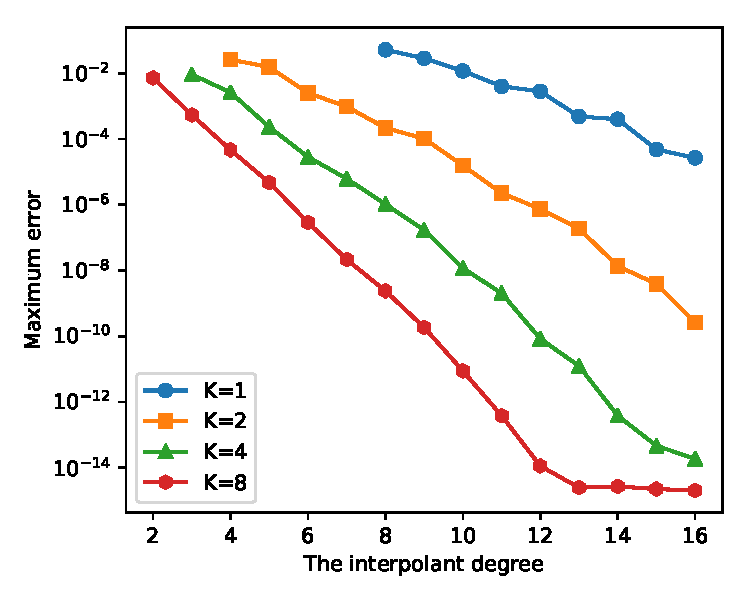
\includegraphics{tex/figures/interpolant_error}
	\fautor
	\label{fig:interpolant_error}
\end{figure}

\begin{figure}
	\centering
	\caption{The interpolation error measured on roots that were found after three Newton's iterations.}
	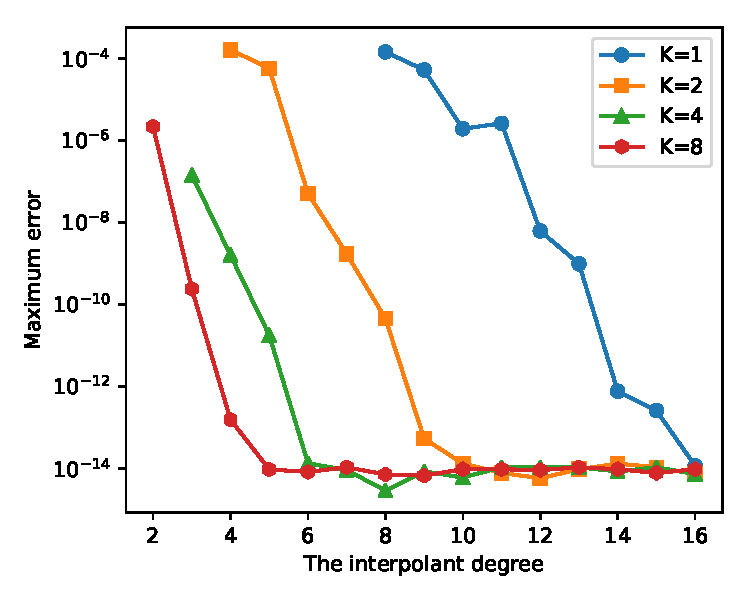
\includegraphics{tex/figures/interpolant_error_after_newton}
	\fautor
	\label{fig:interpolant_error_after_newton}
\end{figure}


\chapter{Maximum Covering by Ellipses with Rotation}
\label{chapter:mcer}
This section introduces the elliptical PMCLP where there is no axis-parallel constraint, that is, the ellipses can be freely rotated. We refer to this problem as \sigla{MCER}{Maximal Covering by Ellipses with Rotation}. In comparison with MCE, this problem introduces a new a new variable which is responsible for determining the rotation angle of every ellipse making MCER a more challenging problem.

\section{Definition}

An instance of the non-axis-parallel is defined exactly like the axis-parallel one on \autoref{chapter:ellipses}. It is given by a set of demand points $\Pp=\{p_1, \dots, p_n\}$, $p_j\in\R^2$; a list of weights $\Ww:=\{w_1, \dots, w_n\}$, with $w_j\in\R_{\ge0}$ being the weight of point $p_j$;
and a set of $m$ axis-parallel ellipses given by their shape parameters $\Rr:=\{(a_1, b_1), \dots, (a_m, b_m)\}$, with $(a_j, b_j)\in\R_{>0}^2$ and $a_j>b_j$.
Additionally, to make the text more clear, we define a set of $m$ ellipses as $\E = \{E_1, \dots, E_m\}$, with $E_j : \R^2\times\R^2 \mapsto \R^2$ being a function that takes the center and angle of rotation where the $j$-th ellipse is located as input, and returns its coverage region.

Given an instance of $MCER$, we define $Q:=(q_1, \dots, q_m) \in \R^{2m}$ to be the centers of each ellipse, $\Theta:=(\theta_1, \dots, \theta_m) \in [0, \pi)^m$ to be the angle of rotation of each ellipse and $E_i(q_i, \theta_i)$ to be the coverage region of ellipse $E_i$ with its center at point $q_i$ rotated by angle $\theta_i$, which is given by \autoref{eq:rotated_ellipse_co}. Therefore MCER is defined as the problem of determining $Q$ and $\Theta$ (placing and rotating each ellipse) to maximize the weight of points covered by the $m$ ellipses, which is given by

\begin{equation}\label{eq:optMCEn}
\max_{Q, \Theta}{w\left(\bigcup_{i=1}^{m} \Pp \cap E_i(q_i, \theta_i)\right)}.
\end{equation}

An additional notation is used on this chapter, $\tilde{E_i}(q_i, \theta_i)$ is defined to be the set of points on the border of $E_i(q_i, \theta_i)$, specially, the operation $\Pp \cap \tilde{E_i}(q_i, \theta_i)$ is used to refer to the set of points from $\Pp$ that lie on the border of $E_i(q_i, \theta_i)$.


\begin{proposicao}\label{lema:mce_2b}
	Let $(\Pp, \E)$ be an instance of MCER. In an optimal solution of MCER, for any $E_j \in \E$, such that $|\Pp \cap E_j(q_j, \theta_j)|\ge2$, there is $q_j'$ such that $\Pp \cap E_j(q_j', \theta_j)=\Pp \cap E_j(q_j, \theta_j)$ and $\Pp \cap \tilde{E_j}(q_j', \theta_j) \ge 2$.
\end{proposicao}

\begin{demonstracao}
	First, the angle of rotation can be ignored as it does not change.
	
	Let $A=\Pp \cap E_j(q_j, \theta_j)$ be the set of points covered by $E_j$ and $X=\cap_{p \in A}E_j(p, \theta_j)$ be the region of intersection of ellipses centered at each point from $A$.

	As it was shown on \autoref{chapter:ellipses}, $X$ is a region that is limited by arcs of ellipses. As this region is the non-empty intersection of more than one ellipse, there are at least two of these arcs that encounter at one point creating a vertex. Selecting any of these vertices as $q_j'$ will make $|\Pp \cap \tilde{E}_j(q_j', \theta_j)| \ge 2$.
	
\end{demonstracao}

What \autoref{lema:mce_2b} is saying is that any optimal solution for MCER can be transformed into another optimal solution where every ellipse covers the same set of points and those which cover more than one point has two points on their border. Also, this equivalent optimal solution can be always achieved by just translating the ellipses. An example is shown on \autoref{fig:ellipse-2-points} for one ellipse.

A lot of the ideas developed in this chapter are based on fixing two points on the border of an ellipse, which is why \autoref{def:feasible_angle} introduces a new notation for angles that an ellipse rotated by it can be translated into a center, such that it contains two fixed points. 

\begin{figure}[H]
	\centering
	\caption{An optimal solution before and after applying \autoref{lema:mce_2b}.}
	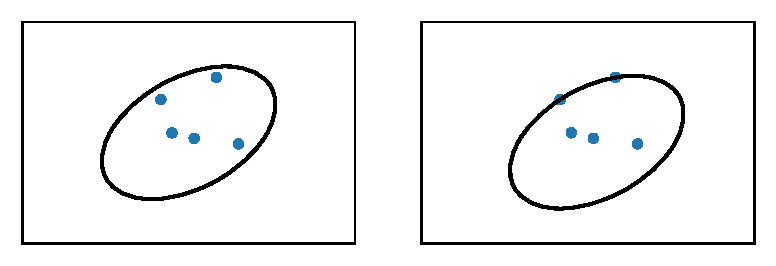
\includegraphics{tex/figures/scripts/ellipse-2-points}
	\fautor
	\label{fig:ellipse-2-points}
\end{figure}

\begin{definicao}\label{def:feasible_angle}
	Let $E$ be an ellipse and $u, v \in \R^2$. An angle $\theta \in [0, \pi)$ is said to be $(E, u, v)$-feasible if there is $q \in \R^2$ such that $\{u, v\} \subset \tilde{E}(q, \theta)$.
\end{definicao}

On \autoref{fig:feasible-angle} two examples for \autoref{def:feasible_angle} are shown. On one of them, an ellipse is rotated by $\pi/4$ and it is located such that it contains the two fixed points on its border. That means $\pi/4$ is a $(E, u, v)$-feasible angle. On the other example, the ellipse is rotated by $\pi/2$ and there is not a center where the ellipse can be placed so it contains the two fixed points--they are too far apart. This makes $\pi/2$ a not $(E, u, v)$-feasible angle.

\begin{figure}
	\centering
	\caption{A $(E, u, v)$-feasible angle and a not $(E, u, v)$-feasible angle.}
	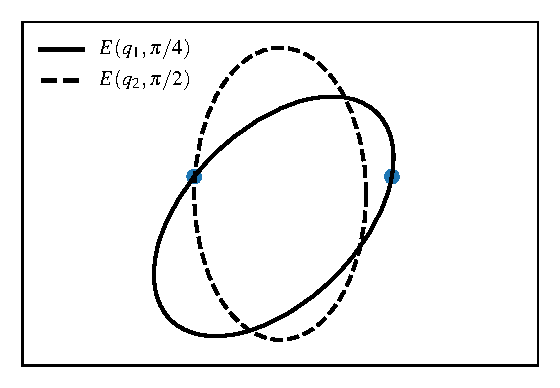
\includegraphics{tex/figures/scripts/feasible-angle}
	\fautor
	\label{fig:feasible-angle}
\end{figure}

\begin{lema}\label{lema:3pnts}
	Let $(\Pp, \E)$ be an instance of MCER, in an optimal solution, for any $E_j \in \E$, such that $|\Pp \cap E_j(q_j, \theta_j)|>2$, at least one of the two cases is true:
	
	\begin{enumerate}
		\item There is $q', \theta'$, and $\{u, v, w\} \subset \Pp \cap E_j(q_j, \theta_j)$, such that $\{u, v, w\} \subset \tilde{E}(q', \theta')$.
		
		\item Let $A=\Pp \cap E_j(q_j, \theta_j)$, and $u, v \in A$ such that there exists $\hat{q}_j$ such that $\{u, v\} \subset \tilde{E_j}(\hat{q}_j, \theta_j)$ and $A \subset E_j(\hat{q}_j, \theta_j)$. Then for any $(E_j, u, v)$-feasible angle $\theta \in [0, 2\pi]$, there exists $\bar{q}_j$ such that $\{u, v\} \subset \tilde{E_j}(\bar{q}_j, \theta)$ and $A \subset E_j(\bar{q}_j, \theta)$.
	\end{enumerate}
\end{lema}

The first case of \autoref{lema:3pnts} is saying that there is another optimal solution which has $E_j$ covering the same set of points, but with three points on its border. 

The second case of \autoref{lema:3pnts} says that after fixing a pair of points on the border of $E_j$ maintaining the covered set, for any angle that allows the two points to stay on the border of $E_j$, there is a center that maintains the covered set the same.

On \autoref{fig:lema-3-points} both cases of \autoref{lema:3pnts} are shown. There, it can be seen that for the second case, it does not matter which feasible angle by which the ellipse is rotated, the third point will always be inside the coverage area. Also, an example of the first case is shown where there are three points lie exactly on the border of the ellipse.

\begin{figure}
	\centering
	\caption{An example of \autoref{lema:3pnts}.}
	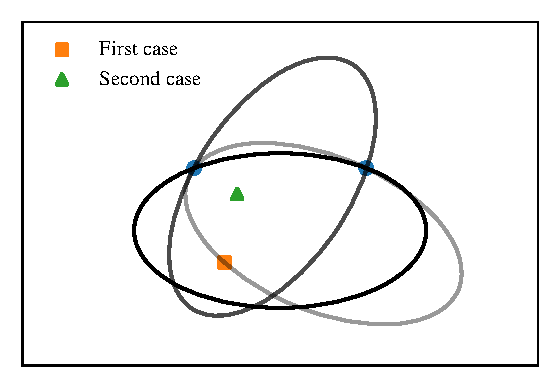
\includegraphics{tex/figures/scripts/lema-3-points}
	\fautor
	\label{fig:lema-3-points}
\end{figure}

The idea to prove \autoref{lema:3pnts} is that after fixing $u, v$ on the border of $E_j$, which is possible by \autoref{lema:mce_2b}, the movement of rotation and translation while keeping $u, v$ on the border is continuous. Because of that, the negation of case two implies case one and vice versa.


If we define an equivalence relation between optimal solutions as: $S_1$ is equivalent to $S_2$ if they both cover the same set of points, we can use \autoref{lema:3pnts} and \autoref{lema:mce_2b} to identify the equivalence classes. Let $S$ be any optimal solution, in $[S]$ (its equivalence class) there is another solution where any ellipse $E_j \in \E$ falls in at least one of the cases below:
\begin{itemize}
	\item $E_j$ covers only one point.
	\item $E_j$ covers more than one point with $u$ and $v$ being on the border of $E_j$. Note that there could be infinitely many of solutions like that, however, \autoref{lema:3pnts} guarantees that any $(E_j, u, v)$-feasible angle yields an equivalent optimal solution.
	\item $E_j$ covers more than two points with three of them on its border.
\end{itemize}

The following two sections will treat the second and third cases (the first case is trivial). Going through every possibility of an ellipse falling in any of the three cases guarantees that an optimal solution is found.

\section{Ellipse by two points}

Let $E$ be an ellipse with shape parameters $(a, b)\in \R^2_{>0}$ and $u, v\in \R^2$, one wants to find a $(E, u, v)$-feasible angle $\theta\in[0,\pi]$ and every center $q\in\R^2$ such that $\{u, v\} \subset \tilde{E}(q, \theta)$.

For a fixed angle, finding every center such that two points are on the border of the ellipse is done on \autoref{chapter:ellipses_intersection}, from there we know that there could be at most $2$ of such centers. The only thing left to be done is finding a feasible angle. It turns out that the angle that makes the major-axis of the ellipse to be aligned with the line that passes through $u$ and $v$ will be a feasible angle if, and only if the set of feasible angles is not empty. This can be seen geometrically as other angles achieve a lesser maximum distance between the two points on the border.

\section{Ellipse by three points}




\chapter{Numerical Experiments}
\label{chapter:numerical}
The goal of this chapter is to show in practice the results of the algorithms for MCE and MCER proposed by us. We first give some implementation details, then we start discuss the solutions obtained for instances proposed in past works, and finally we propose some new instances with the intention of finding the limits of our algorithms.

\section{Implementation}

All the algorithms were implemented using the C++ language, with compiler g++ (G++ 6.3.0). To activate the optimization of compilation we used the -O4 flag.. All the experiments were run in a computer with the following specification:
\begin{itemize}
	\item CPU Intel(R) Core(TM) i7-2600 CPU @ 3.40GHz;
	\item 16Gib of RAM memory;
	\item Linux Operating System: Debian 4.19.5.
\end{itemize}
\subsection{Determining the eigenvalues of a matrix}

In \autoref{algoritmo:e3p}, we assumed that a procedure which returns every eigenvalue of a given square matrix was available. In practice, we used the very famous linear algebra package LAPACK (see \citeonline{lapack} for more details).
LAPACK is a library for the FORTRAN programming language. However, its routines can be made available in a C/C++ environment by simply adding the -llapack linking flag to the compilation. The only remarks, though, are that FORTAN represents matrices in a column-major fashion, and receives parameters only by reference. Therefore, matrices must be transposed before being passed to a routine, and every parameter must receive a pointer to a variable containing its value.

LAPACK offers a routine called ZGEEV that computes every eigenvalue of a complex matrix by using an implementation of the QR algorithm. 
This routine optionally can also be asked to compute the right or left eigenvectors depending on two of its parameters. 
ZGEEV receives in total $14$ parameters, with $4$ of them being used for output. We show a brief description of them in \autoref{tab:zgeev} along with the specification of the value we set each parameter in our implementation.
%\renewcommand{\arraystretch}{1.1}

\begin{table}[H]\label{tab:zgeev}
	\begin{center}
	\begin{tabular}{|c|m{18em}|m{8em}|}
		
		\hline
		\textbf{Parameter} & \multicolumn{1}{c|}{\textbf{Description}} & \multicolumn{1}{c|}{\textbf{Value}}\\
		\hline
		JOBVL&  Indicates whether to compute the left eigenvalues&  'N' (no eigenvectors should be computed)\\
		\hline
		JOBVR&  Indicates whether to compute the right eigenvalues&  'N' (no eigenvectors should be computed)\\
		\hline
		N    &  Order of matrix A &  6\\
		\hline
		A    &  The square matrix whose eigenvalues are to be computed & The companion matrix \\
		\hline
		LDA  &  Leading dimension of A & 6 \\
		\hline
		W    &  The eigenvalues output array &  A complex array of size 6\\
		\hline
		VL   &  The left eigenvectors output array & A complex array of size 1 \\
		\hline
		LDVL &  Leading dimension of VL&  1\\
		\hline
		VR   &  The right eigenvectors output array&  A complex array of size 1\\
		\hline
		LDVR &  Leading dimension of VR&  1\\
		\hline
		WORK &  A workspace for the procedure to utilize&  A complex array of size 12\\
		\hline
		LWORK&  Dimension of WORK &  12\\
		\hline
		RWORK&  A real workspace of size 2N &  A double array of size 12\\
		\hline
		INFO &  An integer containing $0$ if the algorithm was able to compute every eigenvalue &  A pointer to an integer variable\\
		\hline
	\end{tabular}
	\end{center}
	\caption{The ZGEEV's parameter list.}
\end{table}

\subsection{Symbolic Computation}

Symbolic computation is a vast topic, which deals with the problem of solving or manipulating mathematical expressions computationally. 

Back in \autoref{chapter:e3p}, we were faced with the problem of writing the function $\xi$ defined in \autoref{eq:circumscribed_circle_b} as a complex polynomial in the power format by replacing the sine and cosine functions with the identities given by  \autoref{eq:complex_trig_cos} and \autoref{eq:complex_trig_sin}.

As expected, computing the coefficients of that polynomial in terms of the E3P's instance by hand is very challenging; the expressions get too long, and it becomes humanly impossible not to make any mistake. 
For that reason, we resort to Symbolic computation for this task.

In practice, we utilized an external library for Python called SymPy (see \citeonline{sympy} for more information).
This tool can create expressions using arithmetic operators on predefined symbols, numbers, and other expressions. It can also convert expressions into polynomials in the power format, and output them directly into C code. Using these features, we can write $\xi(\theta)(e^{i\theta})^6$ as a polynomial by replacing the sine and cosine functions with expressions for the identities given by  \autoref{eq:complex_trig_cos} and \autoref{eq:complex_trig_sin}, and then import it into our C++ implementation of \autoref{algoritmo:e3p} by printing the polynomial's list of coefficients as C code.

%This can be done by creating a composition of an expression for $\xi(\theta)(e^{i\theta})^6$ with the expressions for $\cos(\theta)$ and $\sin(\theta)$ defined by \autoref{eq:complex_trig_cos} and \autoref{eq:complex_trig_sin}.
%After that, running a command, we can ask SymPy to transform that expression into a polynomial informing it that its variable is $z=e^{i\theta}$. Finally, very conveniently for us, SymPy has a function that outputs expressions directly as C code, which can be used to import the polynomial into our implementation of \autoref{algoritmo:e3p}.

\subsection{Some details and improvements}\label{section:improvements}

To achieve the results that are shown later in this chapter, an efficient implementation of \autoref{algoritmo:mce} and \autoref{algoritmo:mcer} had to be done. Just translating those algorithms into a programming language was not enough to obtain solutions for every instance previously published in \citeonline{andreta}.
Therefore, we present here, some improvements that can be applied to the implementation of those algorithms, which can result in a significant improvement in performance, especially in terms of CPU time.

In both algorithms, a subroutine to construct an ellipse's CLS is called inside the backtracking routine. This can potentially make the same combination of points be considered multiple times.
To avoid this unnecessary computation, points that have already been considered for an ellipse's CLS can be stored, and only new combinations can then be taken into account each time the CLS subroutine is called. 

Another improvement that can be made in the construction of an ellipse's CLS is the elimination of redundant solutions.
Let $(Q, \Theta)$ and $(Q', \Theta')$ be two solutions of MCER. If, for any $j \in \{1, \dots, m\}$, we have $\Pp \cap E_j(q_j', \theta_j') \subset \Pp \cap E(q_j, \theta_j)$, then we can for sure dismiss solution $(Q', \Theta')$.
In our implementation, we use the same tree-like data structure as the one described by \citeonline{andreta} to only keep solutions that are not redundant.

Also, to avoid solving the subproblem E3P in the algorithm for MCER, we can check if the maximum distance between any of the three points is greater than $2a$, where $a$ is an ellipse's semi-major. This is useful because calling \autoref{algoritmo:e3p} for every triplet of points of an instance of MCER can be very expensive.

The last implementation improvement was obtained by keeping an upper-bound, which can be used to skip solutions that are surely not better than the current best solution.
When the backtracking algorithm has the location for the first $j$ ellipses fixed, we want to have an upper-bound for the best solution that can still be found by choosing the location of the $m-j$ remaining ellipses.
Let us consider the case for the MCER's algorithm (the MCE's case is analogous). Let $$z_j = \max_{(q, \theta) \in S_j} w(\Pp \cap E_j(q, \theta)),$$ and $OPT_j$ be the value of the best solution which has the first $j$ ellipses fixed at $(q_1, \theta_1); \dots; (q_j, \theta_j)$. Then, as $z_k$ is the best value that the $k$-th ellipse can contribute to any solution, we get the following inequality
\begin{equation*}
OPT_j \le w\left(\bigcup_{k=1}^{j} \Pp \cap E_k(q_k, \theta_k)\right) + \sum_{k=j+1}^m z_k.
\end{equation*}
This upper-bound is easy to compute as $\{z_1, \dots, z_m\}$ can be preprocessed, and the weight of every point covered so far in the backtrack can be obtained by adding another parameter to the $MCER_{bt}$ procedure.
Let $OPT$ be the current optimal solution, we have that if
\begin{equation}
\label{eq:upper-bound}
w\left(\bigcup_{k=1}^{j} \Pp \cap E_k(q_k, \theta_k)\right) + \sum_{k=j+1}^m z_k \le OPT,
\end{equation}
then $OPT_j \le OPT$, which means that we can skip every solution with the first $j$ ellipses fixed at $(q_1, \theta_1); \dots; (q_j, \theta_j)$.

It is worth pointing out that these improvement suggestions do not have an effect in a possible worst case scenario. We are adopting them in our implementation because they showed good results in practice.
For example, without taking the suggestion given by \autoref{eq:upper-bound}, \autoref{algoritmo:mcer-k} takes nine seconds to obtain an optimal solution for instance AB060, going through \num{336494451} solutions.
In \autoref{tab:mcer-results-ab1}, we show the results of \autoref{algoritmo:mcer-k} implemented with all the improvement suggestions given here; for the instance AB060, the algorithm takes less than one second to return an optimal solution, and evaluates only \num{1809} solutions.

\section{A greedy algorithm}

In \citeonline{church:1974} a simple greedy algorithm was introduced to compare the results obtained by the other algorithms developed by them. We do the same here and define a general greedy algorithm, which follows the same approach as the one in \citeonline{church:1974}, that works for both MCE and MCER.

Let $(\Pp, \Ww, \Rr)$ be an instance of MCE or MCER. Then, at the $j$-th iteration of the algorithm we choose the solution for the first ellipse. Considering $Z_j \subset \Pp$ as the set of uncovered points before the $j$-th iteration. Then, we set the solution for the $j$-th ellipse, as the solution of an instance of MCE-1 or MCER-1 with demand points $Z_j$.
That is the same as choosing, among all the possibilities in the $j$-th ellipse's CLS, the solution which maximizes the weight of covered points in $Z_j$.

\section{Results for known instances}

In this section, we present the results of \autoref{algoritmo:mce-k} and \autoref{algoritmo:mcer-k} for the instances CM1,CM2, CM4, CM5, CM7, CM8 proposed by \citeonline{canbolat}, and for the instances CM3,CM6,CM9 and AB001-AB120 proposed by \citeonline{andreta}.

For each instance, we display the selected ellipses and the income of the found optimal solution. 
We also display some performance metrics with the intention of giving an idea of how much computation had to be done for the algorithms to find an optimal solution. These metrics are: 
the CLS size of every ellipse, the number of nodes in the backtracking tree, the number of leaves corresponding to a solution in the backtracking tree, the CPU time spent on constructing the CLSs, and the total CPU time.
For the algorithms for MCER, we also have a column for the number of E3P subproblems that were solved, not counting the triplet of points which are dismissed by the improvements suggestions given in \autoref{section:improvements}.


\subsection{MCE-$k$}

In \autoref{tab:mce-results-cm}, the results for instances CM1-CM9 are shown. 
The algorithm proposed here showed great results as it was able to obtain optimal solutions in less than one second for every one of the instances CM1-CM9.
Even though the experiments were run in a different environment, we can still say that this is a great improvement compared with the results from \citeonline{andreta}. For example, to obtain an optimal solution for the instance CM9, the method proposed by \citeonline{andreta} took more than thirty minutes.
In \autoref{tab:mce-results-ab1} and \autoref{tab:mce-results-ab2}, we present the results for instances AB001-AB120. The only instance that our algorithm took more than one second to return an optimal solution was AB120, which it took 1.08 second.

In practice, at least for these instances, the bound $\bigO(n^{3m})$ for the algorithm for MCE-$k$ seems to be loose. In instance CM9, for example, this bound says that the number of leaves corresponding to a solution in the backtracking tree should be close to $n^{3m} = (10^2)^{3\times 3} = 10^{18}$, which is very far from the actual number of $649$ such leaves obtained in practice.
This is also the case for the size of the CLSs, which are all very far away from its $\bigO(n^2)$ bound. The greatest CLS size observed was $174$ for instance CM9, which is still very far away from $n^2$, which in this case is $10^4$.
\begin{table}
	\begin{center}
		\resizebox{\textwidth}{!}{%
			
			\begin{tabular}{|cccc|cr|crrrr|}
				\hline
				\multicolumn{4}{|c|}{Instance} & \multicolumn{2}{c|}{Optimal Solution} & \multicolumn{5}{c|}{Performance metrics}\\
				\hline
				
				%%% Second line of header
				
				\multirow{2}{*}{Name} & 
				\multirow{2}{*}{$n$} & 
				\multirow{2}{*}{$m$} & 
				\multirow{2}{*}{$k$} & 
				Selected & 
				\multirow{2}{*}{Income} & 
				CLS size&
				\multicolumn{2}{c}{Backtracking Tree} & 
				\multicolumn{2}{c|}{\centering CPU Time (s)}\\
				& & & & \centering Ellipses & & $|S_k|$ & \# nodes & \# sol. leaves & CLS-MCE & Total\\
				\hline
				CM1&\multirow{3}{*}{\num{25}}&\multirow{3}{*}{\num{3}}&\num{1}&\num{1}\num{2},\num{3},&\num{3.0}&\num{19}&\num{58}&\num{18}&\num{0.00}&\num{0.00}
\\CM2& & &\num{2}&\num{1},\num{2}\num{3},&\num{3.0}&\num{21}&\num{58}&\num{18}&\num{0.00}&\num{0.00}
\\CM3& & &\num{3}&\num{1},\num{2},\num{3}&\num{3.0}&\num{19}&\num{58}&\num{18}&\num{0.00}&\num{0.00}
\\\hline
CM4&\multirow{3}{*}{\num{50}}&\multirow{3}{*}{\num{3}}&\num{1}&\num{1}\num{2},\num{3},&\num{10.0}&\num{43}&\num{141}&\num{50}&\num{0.00}&\num{0.00}
\\CM5& & &\num{2}&\num{1},\num{2}\num{3},&\num{10.0}&\num{47}&\num{141}&\num{50}&\num{0.00}&\num{0.00}
\\CM6& & &\num{3}&\num{1},\num{2},\num{3}&\num{10.0}&\num{50}&\num{141}&\num{50}&\num{0.00}&\num{0.00}
\\\hline
CM7&\multirow{3}{*}{\num{100}}&\multirow{3}{*}{\num{3}}&\num{1}&\num{1}\num{2},\num{3},&\num{25.0}&\num{101}&\num{924}&\num{687}&\num{0.02}&\num{0.02}
\\CM8& & &\num{2}&\num{1},\num{2}\num{3},&\num{25.0}&\num{135}&\num{924}&\num{687}&\num{0.02}&\num{0.02}
\\CM9& & &\num{3}&\num{1},\num{2},\num{3}&\num{25.0}&\num{174}&\num{924}&\num{687}&\num{0.02}&\num{0.02}
\\
				\hline
				
			\end{tabular}
		}
		\caption{Solutions of MCE-$k$ for instances CM1-CM9.}
		\label{tab:mce-results-cm}
	\end{center}
\end{table}

\begin{table}
	\begin{center}
		\resizebox{0.85\textwidth}{!}{%
			
			\begin{tabular}{|cccc|cr|crrrr|}
				\hline
				\multicolumn{4}{|c|}{Instance} & \multicolumn{2}{c|}{Optimal Solution} & \multicolumn{5}{c|}{Performance metrics}\\
				\hline
				
				%%% Second line of header
				
			\multirow{2}{*}{Name} & 
			\multirow{2}{*}{$n$} & 
			\multirow{2}{*}{$m$} & 
			\multirow{2}{*}{$k$} & 
			Selected & 
			\multirow{2}{*}{Income} & 
			CLS size&
			\multicolumn{2}{c}{Backtracking Tree} & 
			\multicolumn{2}{c|}{\centering CPU Time (s)}\\
			& & & & \centering Ellipses & & $|S_k|$ & \# nodes & \# sol. leaves & CLS-MCE & Total\\
				\hline
				AB001&\multirow{0}{*}{\num{10}}&\multirow{0}{*}{\num{3}}&\num{1}&\num{2}&\num{1.4}&\multirow{0}{*}{\num{10}}&\num{32}&\num{11}&\num{0.00}&\num{0.00}
\\AB002& & &\num{2}&\num{2},\num{3}&\num{2.3}& &\num{66}&\num{8}&\num{0.00}&\num{0.00}
\\AB003& & &\num{3}&\num{1},\num{2},\num{3}&\num{2.8}& &\num{162}&\num{6}&\num{0.00}&\num{0.00}
\\\hline
AB004&\multirow{3}{*}{\num{10}}&\multirow{3}{*}{\num{4}}&\num{1}&\num{4}&\num{0.9}&\multirow{3}{*}{\num{10}}&\num{41}&\num{10}&\num{0.00}&\num{0.00}
\\AB005& & &\num{2}&\num{2},\num{4}&\num{1.4}& &\num{159}&\num{98}&\num{0.00}&\num{0.00}
\\AB006& & &\num{3}&\num{2},\num{3},\num{4}&\num{1.8}& &\num{312}&\num{112}&\num{0.00}&\num{0.00}
\\AB007& & &\num{4}&\num{1},\num{2},\num{3},\num{4}&\num{1.0}& &\num{1150}&\num{60}&\num{0.00}&\num{0.00}
\\\hline
AB008&\multirow{4}{*}{\num{10}}&\multirow{4}{*}{\num{5}}&\num{1}&\num{5}&\num{0.9}&\multirow{4}{*}{\num{10}}&\num{54}&\num{10}&\num{0.00}&\num{0.00}
\\AB009& & &\num{2}&\num{3},\num{5}&\num{1.4}& &\num{172}&\num{98}&\num{0.00}&\num{0.00}
\\AB010& & &\num{3}&\num{3},\num{4},\num{5}&\num{1.8}& &\num{286}&\num{56}&\num{0.00}&\num{0.00}
\\AB011& & &\num{4}&\num{2},\num{3},\num{4},\num{5}&\num{1.0}& &\num{1492}&\num{120}&\num{0.00}&\num{0.00}
\\AB012& & &\num{5}&\num{1},\num{2},\num{3},\num{4},\num{5}&\num{-1.5}& &\num{8693}&\num{7}&\num{0.00}&\num{0.00}
\\\hline
AB013&\multirow{5}{*}{\num{20}}&\multirow{5}{*}{\num{3}}&\num{1}&\num{2}&\num{1.4}&\multirow{5}{*}{\num{20}}&\num{58}&\num{21}&\num{0.00}&\num{0.00}
\\AB014& & &\num{2}&\num{2},\num{3}&\num{2.3}& &\num{198}&\num{18}&\num{0.00}&\num{0.00}
\\AB015& & &\num{3}&\num{1},\num{2},\num{3}&\num{2.8}& &\num{573}&\num{16}&\num{0.00}&\num{0.00}
\\\hline
AB016&\multirow{3}{*}{\num{20}}&\multirow{3}{*}{\num{4}}&\num{1}&\num{2}&\num{1.5}&\multirow{3}{*}{\num{20}}&\num{73}&\num{22}&\num{0.00}&\num{0.00}
\\AB017& & &\num{2}&\num{2},\num{3}&\num{2.9}& &\num{192}&\num{36}&\num{0.00}&\num{0.00}
\\AB018& & &\num{3}&\num{2},\num{3},\num{4}&\num{3.8}& &\num{645}&\num{15}&\num{0.00}&\num{0.00}
\\AB019& & &\num{4}&\num{1},\num{2},\num{3},\num{4}&\num{4.0}& &\num{6331}&\num{37}&\num{0.00}&\num{0.00}
\\\hline
AB020&\multirow{4}{*}{\num{20}}&\multirow{4}{*}{\num{5}}&\num{1}&\num{4}&\num{2.4}&\multirow{4}{*}{\num{20}}&\num{82}&\num{21}&\num{0.00}&\num{0.00}
\\AB021& & &\num{2}&\num{3},\num{4}&\num{3.9}& &\num{131}&\num{18}&\num{0.00}&\num{0.00}
\\AB022& & &\num{3}&\num{3},\num{4},\num{5}&\num{4.8}& &\num{569}&\num{29}&\num{0.00}&\num{0.00}
\\AB023& & &\num{4}&\num{2},\num{3},\num{4},\num{5}&\num{4.0}& &\num{8681}&\num{108}&\num{0.00}&\num{0.00}
\\AB024& & &\num{5}&\num{1},\num{2},\num{3},\num{4},\num{5}&\num{2.5}& &\num{54810}&\num{229}&\num{0.00}&\num{0.00}
\\\hline
AB025&\multirow{5}{*}{\num{30}}&\multirow{5}{*}{\num{3}}&\num{1}&\num{1}&\num{2.5}&\multirow{5}{*}{\num{27}}&\num{74}&\num{29}&\num{0.00}&\num{0.00}
\\AB026& & &\num{2}&\num{1},\num{2}&\num{4.9}& &\num{166}&\num{50}&\num{0.00}&\num{0.00}
\\AB027& & &\num{3}&\num{1},\num{2},\num{3}&\num{6.8}& &\num{769}&\num{22}&\num{0.00}&\num{0.00}
\\\hline
AB028&\multirow{3}{*}{\num{30}}&\multirow{3}{*}{\num{4}}&\num{1}&\num{2}&\num{2.5}&\multirow{3}{*}{\num{28}}&\num{101}&\num{30}&\num{0.00}&\num{0.00}
\\AB029& & &\num{2}&\num{2},\num{3}&\num{4.9}& &\num{420}&\num{52}&\num{0.00}&\num{0.00}
\\AB030& & &\num{3}&\num{1},\num{2},\num{3}&\num{6.1}& &\num{1933}&\num{109}&\num{0.00}&\num{0.00}
\\AB031& & &\num{4}&\num{1},\num{2},\num{3},\num{4}&\num{7.0}& &\num{16219}&\num{456}&\num{0.00}&\num{0.00}
\\\hline
AB032&\multirow{4}{*}{\num{30}}&\multirow{4}{*}{\num{5}}&\num{1}&\num{3}&\num{2.5}&\multirow{4}{*}{\num{27}}&\num{119}&\num{29}&\num{0.00}&\num{0.00}
\\AB033& & &\num{2}&\num{3},\num{4}&\num{4.9}& &\num{472}&\num{49}&\num{0.00}&\num{0.00}
\\AB034& & &\num{3}&\num{2},\num{3},\num{4}&\num{7.1}& &\num{1621}&\num{22}&\num{0.00}&\num{0.00}
\\AB035& & &\num{4}&\num{2},\num{3},\num{4},\num{5}&\num{9.0}& &\num{12208}&\num{17}&\num{0.00}&\num{0.00}
\\AB036& & &\num{5}&\num{1},\num{2},\num{3},\num{4},\num{5}&\num{9.5}& &\num{179281}&\num{53}&\num{0.00}&\num{0.01}
\\\hline
AB037&\multirow{5}{*}{\num{40}}&\multirow{5}{*}{\num{3}}&\num{1}&\num{1}&\num{2.5}&\multirow{5}{*}{\num{37}}&\num{102}&\num{39}&\num{0.00}&\num{0.00}
\\AB038& & &\num{2}&\num{1},\num{2}&\num{4.9}& &\num{315}&\num{70}&\num{0.00}&\num{0.00}
\\AB039& & &\num{3}&\num{1},\num{2},\num{3}&\num{6.8}& &\num{1441}&\num{65}&\num{0.00}&\num{0.00}
\\\hline
AB040&\multirow{3}{*}{\num{40}}&\multirow{3}{*}{\num{4}}&\num{1}&\num{1}&\num{5.2}&\multirow{3}{*}{\num{37}}&\num{125}&\num{40}&\num{0.00}&\num{0.00}
\\AB041& & &\num{2}&\num{1},\num{4}&\num{7.1}& &\num{393}&\num{97}&\num{0.00}&\num{0.00}
\\AB042& & &\num{3}&\num{1},\num{2},\num{4}&\num{8.6}& &\num{2904}&\num{116}&\num{0.00}&\num{0.00}
\\AB043& & &\num{4}&\num{1},\num{2},\num{3},\num{4}&\num{10.0}& &\num{28554}&\num{296}&\num{0.00}&\num{0.00}
\\\hline
AB044&\multirow{4}{*}{\num{40}}&\multirow{4}{*}{\num{5}}&\num{1}&\num{3}&\num{3.5}&\multirow{4}{*}{\num{36}}&\num{148}&\num{38}&\num{0.00}&\num{0.00}
\\AB045& & &\num{2}&\num{1},\num{3}&\num{7.0}& &\num{754}&\num{68}&\num{0.00}&\num{0.00}
\\AB046& & &\num{3}&\num{1},\num{2},\num{3}&\num{9.2}& &\num{3847}&\num{61}&\num{0.00}&\num{0.00}
\\AB047& & &\num{4}&\num{1},\num{2},\num{3},\num{5}&\num{11.1}& &\num{33846}&\num{99}&\num{0.00}&\num{0.00}
\\AB048& & &\num{5}&\num{1},\num{2},\num{3},\num{4},\num{5}&\num{12.5}& &\num{524078}&\num{60}&\num{0.00}&\num{0.01}
\\\hline
AB049&\multirow{5}{*}{\num{50}}&\multirow{5}{*}{\num{3}}&\num{1}&\num{1}&\num{5.5}&\multirow{5}{*}{\num{42}}&\num{120}&\num{44}&\num{0.00}&\num{0.00}
\\AB050& & &\num{2}&\num{1},\num{2}&\num{7.9}& &\num{605}&\num{278}&\num{0.00}&\num{0.00}
\\AB051& & &\num{3}&\num{1},\num{2},\num{3}&\num{9.8}& &\num{2429}&\num{436}&\num{0.00}&\num{0.00}
\\\hline
AB052&\multirow{3}{*}{\num{50}}&\multirow{3}{*}{\num{4}}&\num{1}&\num{1}&\num{5.2}&\multirow{3}{*}{\num{46}}&\num{161}&\num{49}&\num{0.00}&\num{0.00}
\\AB053& & &\num{2}&\num{1},\num{2}&\num{8.7}& &\num{590}&\num{130}&\num{0.00}&\num{0.00}
\\AB054& & &\num{3}&\num{1},\num{2},\num{3}&\num{11.1}& &\num{3420}&\num{512}&\num{0.00}&\num{0.00}
\\AB055& & &\num{4}&\num{1},\num{2},\num{3},\num{4}&\num{13.0}& &\num{48977}&\num{1181}&\num{0.00}&\num{0.00}
\\\hline
AB056&\multirow{4}{*}{\num{50}}&\multirow{4}{*}{\num{5}}&\num{1}&\num{1}&\num{3.5}&\multirow{4}{*}{\num{44}}&\num{209}&\num{46}&\num{0.00}&\num{0.00}
\\AB057& & &\num{2}&\num{1},\num{4}&\num{6.9}& &\num{1650}&\num{126}&\num{0.00}&\num{0.00}
\\AB058& & &\num{3}&\num{1},\num{3},\num{4}&\num{9.4}& &\num{8061}&\num{656}&\num{0.00}&\num{0.01}
\\AB059& & &\num{4}&\num{1},\num{2},\num{3},\num{4}&\num{11.6}& &\num{71184}&\num{2016}&\num{0.00}&\num{0.01}
\\AB060& & &\num{5}&\num{1},\num{2},\num{3},\num{4},\num{5}&\num{13.5}& &\num{1971099}&\num{649}&\num{0.00}&\num{0.05}
\\
				\hline
				
			\end{tabular}
		}
		\caption{Solutions of MCE-$k$ for instances AB001-AB060.}
		\label{tab:mce-results-ab1}
	\end{center}
\end{table}

\begin{table}
	\begin{center}
		\resizebox{0.85\textwidth}{!}{%
			
			\begin{tabular}{|cccc|cr|crrrr|}
				\hline
				\multicolumn{4}{|c|}{Instance} & \multicolumn{2}{c|}{Optimal Solution} & \multicolumn{5}{c|}{Performance metrics}\\
				\hline
				
				%%% Second line of header
\multirow{2}{*}{Name} & 
\multirow{2}{*}{$n$} & 
\multirow{2}{*}{$m$} & 
\multirow{2}{*}{$k$} & 
Selected & 
\multirow{2}{*}{Income} & 
CLS size&
\multicolumn{2}{c}{Backtracking Tree} & 
\multicolumn{2}{c|}{\centering CPU Time (s)}\\
& & & & \centering Ellipses & & $|S_k|$ & \# nodes & \#sol. leaves & CLS-MCE & Total\\
				\hline
				AB061&\multirow{3}{*}{\num{60}}&\multirow{3}{*}{\num{3}}&\num{1}&\num{1}&\num{3.5}&\num{38}&\num{140}&\num{56}&\num{0.00}&\num{0.00}
\\AB062& & &\num{2}&\num{1},\num{2}&\num{5.9}&\num{41}&\num{440}&\num{103}&\num{0.00}&\num{0.00}
\\AB063& & &\num{3}&\num{1},\num{2},\num{3}&\num{7.8}&\num{54}&\num{2622}&\num{48}&\num{0.00}&\num{0.00}
\\\hline
AB064&\multirow{4}{*}{\num{60}}&\multirow{4}{*}{\num{4}}&\num{1}&\num{1}&\num{5.2}&\num{51}&\num{196}&\num{54}&\num{0.00}&\num{0.00}
\\AB065& & &\num{2}&\num{1},\num{2}&\num{8.7}&\num{44}&\num{1044}&\num{98}&\num{0.00}&\num{0.00}
\\AB066& & &\num{3}&\num{1},\num{2},\num{3}&\num{12.1}&\num{39}&\num{4275}&\num{130}&\num{0.00}&\num{0.00}
\\AB067& & &\num{4}&\num{1},\num{2},\num{3},\num{4}&\num{14.0}&\num{51}&\num{90366}&\num{77}&\num{0.00}&\num{0.01}
\\\hline
AB068&\multirow{5}{*}{\num{60}}&\multirow{5}{*}{\num{5}}&\num{1}&\num{3}&\num{4.5}&\num{62}&\num{267}&\num{54}&\num{0.01}&\num{0.01}
\\AB069& & &\num{2}&\num{1},\num{3}&\num{9.0}&\num{59}&\num{3479}&\num{102}&\num{0.01}&\num{0.01}
\\AB070& & &\num{3}&\num{1},\num{3},\num{4}&\num{12.4}&\num{42}&\num{25920}&\num{663}&\num{0.00}&\num{0.01}
\\AB071& & &\num{4}&\num{1},\num{2},\num{3},\num{4}&\num{14.6}&\num{43}&\num{198004}&\num{1603}&\num{0.01}&\num{0.01}
\\AB072& & &\num{5}&\num{1},\num{2},\num{3},\num{4},\num{5}&\num{16.5}&\num{52}&\num{5075488}&\num{1089}&\num{0.01}&\num{0.11}
\\\hline
AB073&\multirow{3}{*}{\num{70}}&\multirow{3}{*}{\num{3}}&\num{1}&\num{1}&\num{4.5}&\num{54}&\num{168}&\num{61}&\num{0.00}&\num{0.00}
\\AB074& & &\num{2}&\num{1},\num{2}&\num{7.9}&\num{48}&\num{370}&\num{111}&\num{0.00}&\num{0.00}
\\AB075& & &\num{3}&\num{1},\num{2},\num{3}&\num{9.8}&\num{59}&\num{3725}&\num{51}&\num{0.00}&\num{0.00}
\\\hline
AB076&\multirow{4}{*}{\num{70}}&\multirow{4}{*}{\num{4}}&\num{1}&\num{1}&\num{5.2}&\num{55}&\num{212}&\num{63}&\num{0.00}&\num{0.00}
\\AB077& & &\num{2}&\num{1},\num{2}&\num{9.7}&\num{43}&\num{696}&\num{114}&\num{0.01}&\num{0.01}
\\AB078& & &\num{3}&\num{1},\num{2},\num{3}&\num{13.1}&\num{43}&\num{5080}&\num{102}&\num{0.00}&\num{0.00}
\\AB079& & &\num{4}&\num{1},\num{2},\num{3},\num{4}&\num{16.0}&\num{60}&\num{113819}&\num{46}&\num{0.00}&\num{0.01}
\\\hline
AB080&\multirow{5}{*}{\num{70}}&\multirow{5}{*}{\num{5}}&\num{1}&\num{1}&\num{5.5}&\num{68}&\num{282}&\num{59}&\num{0.01}&\num{0.01}
\\AB081& & &\num{2}&\num{1},\num{3}&\num{10.0}&\num{53}&\num{2178}&\num{209}&\num{0.01}&\num{0.01}
\\AB082& & &\num{3}&\num{1},\num{2},\num{3}&\num{14.2}&\num{47}&\num{9827}&\num{238}&\num{0.01}&\num{0.01}
\\AB083& & &\num{4}&\num{1},\num{2},\num{3},\num{4}&\num{17.6}&\num{43}&\num{130690}&\num{380}&\num{0.01}&\num{0.01}
\\AB084& & &\num{5}&\num{1},\num{2},\num{3},\num{4},\num{5}&\num{19.5}&\num{55}&\num{5256003}&\num{882}&\num{0.01}&\num{0.12}
\\\hline
AB085&\multirow{3}{*}{\num{80}}&\multirow{3}{*}{\num{3}}&\num{1}&\num{1}&\num{4.5}&\num{66}&\num{185}&\num{67}&\num{0.00}&\num{0.00}
\\AB086& & &\num{2}&\num{1},\num{2}&\num{7.9}&\num{47}&\num{351}&\num{122}&\num{0.00}&\num{0.00}
\\AB087& & &\num{3}&\num{1},\num{2},\num{3}&\num{10.8}&\num{65}&\num{3368}&\num{56}&\num{0.00}&\num{0.00}
\\\hline
AB088&\multirow{4}{*}{\num{80}}&\multirow{4}{*}{\num{4}}&\num{1}&\num{1}&\num{7.2}&\num{83}&\num{271}&\num{71}&\num{0.01}&\num{0.01}
\\AB089& & &\num{2}&\num{1},\num{2}&\num{12.7}&\num{52}&\num{1021}&\num{131}&\num{0.01}&\num{0.01}
\\AB090& & &\num{3}&\num{1},\num{2},\num{3}&\num{16.1}&\num{57}&\num{9345}&\num{240}&\num{0.01}&\num{0.01}
\\AB091& & &\num{4}&\num{1},\num{2},\num{3},\num{4}&\num{18.0}&\num{68}&\num{213419}&\num{54}&\num{0.01}&\num{0.01}
\\\hline
AB092&\multirow{5}{*}{\num{80}}&\multirow{5}{*}{\num{5}}&\num{1}&\num{2}&\num{6.2}&\num{90}&\num{377}&\num{77}&\num{0.01}&\num{0.01}
\\AB093& & &\num{2}&\num{2},\num{3}&\num{10.7}&\num{77}&\num{4729}&\num{143}&\num{0.01}&\num{0.01}
\\AB094& & &\num{3}&\num{1},\num{2},\num{3}&\num{15.2}&\num{69}&\num{22942}&\num{335}&\num{0.01}&\num{0.01}
\\AB095& & &\num{4}&\num{1},\num{2},\num{3},\num{4}&\num{18.6}&\num{55}&\num{394218}&\num{236}&\num{0.01}&\num{0.02}
\\AB096& & &\num{5}&\num{1},\num{2},\num{3},\num{4},\num{5}&\num{19.5}&\num{74}&\num{20297007}&\num{161}&\num{0.01}&\num{0.44}
\\\hline
AB097&\multirow{3}{*}{\num{90}}&\multirow{3}{*}{\num{3}}&\num{1}&\num{1}&\num{5.5}&\num{77}&\num{223}&\num{78}&\num{0.00}&\num{0.00}
\\AB098& & &\num{2}&\num{1},\num{2}&\num{9.9}&\num{63}&\num{488}&\num{144}&\num{0.00}&\num{0.00}
\\AB099& & &\num{3}&\num{1},\num{2},\num{3}&\num{11.8}&\num{76}&\num{6399}&\num{67}&\num{0.01}&\num{0.01}
\\\hline
AB100&\multirow{4}{*}{\num{90}}&\multirow{4}{*}{\num{4}}&\num{1}&\num{1}&\num{6.2}&\num{87}&\num{303}&\num{82}&\num{0.01}&\num{0.01}
\\AB101& & &\num{2}&\num{1},\num{2}&\num{10.7}&\num{68}&\num{1213}&\num{226}&\num{0.01}&\num{0.01}
\\AB102& & &\num{3}&\num{1},\num{2},\num{3}&\num{14.1}&\num{58}&\num{7224}&\num{210}&\num{0.01}&\num{0.01}
\\AB103& & &\num{4}&\num{1},\num{2},\num{3},\num{4}&\num{17.0}&\num{79}&\num{310421}&\num{65}&\num{0.01}&\num{0.02}
\\\hline
AB104&\multirow{5}{*}{\num{90}}&\multirow{5}{*}{\num{5}}&\num{1}&\num{2}&\num{8.2}&\num{130}&\num{429}&\num{75}&\num{0.01}&\num{0.01}
\\AB105& & &\num{2}&\num{2},\num{3}&\num{12.7}&\num{96}&\num{8958}&\num{278}&\num{0.01}&\num{0.01}
\\AB106& & &\num{3}&\num{1},\num{2},\num{3}&\num{16.2}&\num{61}&\num{82416}&\num{251}&\num{0.01}&\num{0.01}
\\AB107& & &\num{4}&\num{1},\num{2},\num{3},\num{4}&\num{19.6}&\num{58}&\num{849156}&\num{6699}&\num{0.01}&\num{0.04}
\\AB108& & &\num{5}&\num{1},\num{2},\num{3},\num{4},\num{5}&\num{21.5}&\num{72}&\num{23218619}&\num{13225}&\num{0.01}&\num{0.53}
\\\hline
AB109&\multirow{3}{*}{\num{100}}&\multirow{3}{*}{\num{3}}&\num{1}&\num{1}&\num{5.5}&\num{90}&\num{256}&\num{85}&\num{0.01}&\num{0.01}
\\AB110& & &\num{2}&\num{1},\num{2}&\num{10.9}&\num{76}&\num{487}&\num{158}&\num{0.01}&\num{0.01}
\\AB111& & &\num{3}&\num{1},\num{2},\num{3}&\num{13.8}&\num{83}&\num{8718}&\num{74}&\num{0.01}&\num{0.01}
\\\hline
AB112&\multirow{4}{*}{\num{100}}&\multirow{4}{*}{\num{4}}&\num{1}&\num{1}&\num{7.2}&\num{119}&\num{350}&\num{81}&\num{0.01}&\num{0.01}
\\AB113& & &\num{2}&\num{1},\num{2}&\num{12.7}&\num{80}&\num{1528}&\num{222}&\num{0.01}&\num{0.01}
\\AB114& & &\num{3}&\num{1},\num{2},\num{3}&\num{17.1}&\num{62}&\num{9376}&\num{205}&\num{0.01}&\num{0.01}
\\AB115& & &\num{4}&\num{1},\num{2},\num{3},\num{4}&\num{20.0}&\num{78}&\num{395929}&\num{63}&\num{0.01}&\num{0.02}
\\\hline
AB116&\multirow{5}{*}{\num{100}}&\multirow{5}{*}{\num{5}}&\num{1}&\num{1}&\num{8.5}&\num{142}&\num{508}&\num{87}&\num{0.01}&\num{0.01}
\\AB117& & &\num{2}&\num{1},\num{3}&\num{16.0}&\num{119}&\num{5466}&\num{162}&\num{0.02}&\num{0.02}
\\AB118& & &\num{3}&\num{1},\num{2},\num{3}&\num{22.2}&\num{76}&\num{30950}&\num{151}&\num{0.01}&\num{0.02}
\\AB119& & &\num{4}&\num{1},\num{2},\num{3},\num{4}&\num{25.6}&\num{74}&\num{821985}&\num{196}&\num{0.01}&\num{0.04}
\\AB120& & &\num{5}&\num{1},\num{2},\num{3},\num{4},\num{5}&\num{27.5}&\num{84}&\num{50526278}&\num{118}&\num{0.02}&\num{1.08}
\\
				\hline
				
			\end{tabular}
		}
		\caption{Solutions of MCE-$k$ for instances AB061-AB120.}
		\label{tab:mce-results-ab2}
	\end{center}
\end{table}

\subsection{MCER-$k$}

Two methods for MCER-$k$ were developed in \citeonline{andreta}: a deterministic method using global optimization, and a heuristic-stochastic method also using a global optimization, but taking the first found solution as a global optimizer.
The deterministic method could not find solutions for every instance within a specified time limit, however, comparing with the results of our algorithm, which are displayed in \autoref{tab:mcer-results-cm} for instances CM1-CM9, and in \autoref{tab:mcer-results-ab1} and \autoref{tab:mcer-results-ab2} for isntances AB001-AB120, we could observe that the heuristic method did find an optimal solution for every instance.

In general, our algorithm took much lower CPU time to return an optimal solution when compared with the heuristic method developed by \citeonline{andreta}. For example, for instance CM9 it ran for more than six hours, while our implementation of \autoref{algoritmo:mcer-k} obtained an optimal solution in less than twenty seconds.

We can give the same remarks about the bounds for the algorithm and the CLS size as we did when analyzing the numerical results of MCE-$k$. Notice that, the greatest CLS size was $701$ obtained for instances CM7-CM9, which is very far away from its bound $\bigO(n^3)$, which in this case is $10^6$. By \autoref{th:mcer}, for MCER, the bound for the number of solutions that need to be considered for an optimal one to be found is $\bigO(n^{3m})$, in instance AB120, for example, the number of visited solutions is only $120$, which is way lower than $100^{15}$.

\begin{table}
	\begin{center}
		\resizebox{\textwidth}{!}{%
			
			\begin{tabular}{|cccc|cr|crrrrr|}
				\hline
				\multicolumn{4}{|c|}{Instance} & \multicolumn{2}{c|}{Optimal Solution} & \multicolumn{6}{c|}{Performance metrics}\\
				\hline
				
				%%% Second line of header
				
				\multirow{2}{*}{Name} & 
				\multirow{2}{*}{$n$} & 
				\multirow{2}{*}{$m$} & 
				\multirow{2}{*}{$k$} & 
				Selected & 
				\multirow{2}{*}{Income} & 
				CLS size&
				\# E3P&
				\multicolumn{2}{c}{Backtracking Tree} & 
				\multicolumn{2}{c|}{\centering CPU Time (s)}\\
				& & & & \centering Ellipses & & $|S_k|$ & subproblems & \# nodes & \#sol leaves & CLS-MCER & Total\\
				
				%%%
				%%%
				
				\hline
				CM1&\multirow{3}{*}{\num{25}}&\multirow{3}{*}{\num{3}}&\num{1}&\num{1}&\num{2.0}&\num{27}&\num{480}&\num{82}&\num{27}&\num{0.09}&\num{0.09}
\\CM2& & &\num{2}&\num{1},\num{2}&\num{4.8}&\num{24}&\num{480}&\num{124}&\num{48}&\num{0.09}&\num{0.09}
\\CM3& & &\num{3}&\num{1},\num{2},\num{3}&\num{5.0}&\num{37}&\num{480}&\num{224}&\num{148}&\num{0.09}&\num{0.09}
\\\hline
CM4&\multirow{3}{*}{\num{50}}&\multirow{3}{*}{\num{3}}&\num{1}&\num{1}&\num{4.0}&\num{70}&\num{3427}&\num{211}&\num{70}&\num{0.62}&\num{0.62}
\\CM5& & &\num{2}&\num{1},\num{2}&\num{9.8}&\num{89}&\num{3427}&\num{427}&\num{178}&\num{0.62}&\num{0.62}
\\CM6& & &\num{3}&\num{1},\num{2},\num{3}&\num{13.0}&\num{111}&\num{3427}&\num{582}&\num{333}&\num{0.63}&\num{0.63}
\\\hline
CM7&\multirow{3}{*}{\num{100}}&\multirow{3}{*}{\num{3}}&\num{1}&\num{1}&\num{8.0}&\num{201}&\num{32242}&\num{604}&\num{201}&\num{7.85}&\num{7.85}
\\CM8& & &\num{2}&\num{1},\num{2}&\num{17.8}&\num{369}&\num{32242}&\num{1678}&\num{738}&\num{7.88}&\num{7.88}
\\CM9& & &\num{3}&\num{1},\num{2},\num{3}&\num{28.0}&\num{701}&\num{32242}&\num{4438}&\num{3498}&\num{7.83}&\num{7.86}
\\
				\hline
				
			\end{tabular}
		}
		\caption{Solutions of MCER-$k$ for instances CM1-CM9.}
		\label{tab:mcer-results-cm}
	\end{center}
\end{table}

\begin{table}
	\begin{center}
		\resizebox{\textwidth}{!}{%
			
			\begin{tabular}{|cccc|cr|crrrrr|}
				\hline
\multicolumn{4}{|c|}{Instance} & \multicolumn{2}{c|}{Optimal Solution} & \multicolumn{6}{c|}{Performance metrics}\\
\hline

%%% Second line of header

\multirow{2}{*}{Name} & 
\multirow{2}{*}{$n$} & 
\multirow{2}{*}{$m$} & 
\multirow{2}{*}{$k$} & 
Selected & 
\multirow{2}{*}{Income} & 
CLS size&
\# E3P&
\multicolumn{2}{c}{Backtracking Tree} & 
\multicolumn{2}{c|}{\centering CPU Time (s)}\\
& & & & \centering Ellipses & & $|S_k|$ & subproblems & \# nodes & \#sol leaves & CLS-MCER & Total\\
				
				%%%
				%%%
				
				
				\hline
				AB001&\multirow{3}{*}{\num{10}}&\multirow{3}{*}{\num{3}}&\num{1}&\num{1}\num{2},\num{3},&\num{2.8}&\num{9}&\num{2}&\num{23}&\num{6}&\num{0.00}&\num{0.00}
\\AB002& & &\num{2}&\num{1},\num{2}\num{3},&\num{2.8}&\num{9}&\num{2}&\num{23}&\num{6}&\num{0.00}&\num{0.00}
\\AB003& & &\num{3}&\num{1},\num{2},\num{3}&\num{2.8}&\num{10}&\num{2}&\num{23}&\num{6}&\num{0.00}&\num{0.00}
\\\hline
AB004&\multirow{4}{*}{\num{10}}&\multirow{4}{*}{\num{4}}&\num{1}&\num{1}\num{2},\num{3},\num{4},&\num{2.0}&\num{8}&\num{2}&\num{24}&\num{4}&\num{0.00}&\num{0.00}
\\AB005& & &\num{2}&\num{1},\num{2}\num{3},\num{4},&\num{2.0}&\num{8}&\num{2}&\num{24}&\num{4}&\num{0.00}&\num{0.00}
\\AB006& & &\num{3}&\num{1},\num{2},\num{3}\num{4},&\num{2.0}&\num{8}&\num{2}&\num{24}&\num{4}&\num{0.00}&\num{0.00}
\\AB007& & &\num{4}&\num{1},\num{2},\num{3},\num{4}&\num{2.0}&\num{10}&\num{2}&\num{24}&\num{4}&\num{0.00}&\num{0.00}
\\\hline
AB008&\multirow{5}{*}{\num{10}}&\multirow{5}{*}{\num{5}}&\num{1}&\num{1}\num{2},\num{3},\num{4},\num{5},&\num{-0.5}&\num{12}&\num{34}&\num{157}&\num{2}&\num{0.01}&\num{0.01}
\\AB009& & &\num{2}&\num{1},\num{2}\num{3},\num{4},\num{5},&\num{-0.5}&\num{12}&\num{34}&\num{157}&\num{2}&\num{0.01}&\num{0.01}
\\AB010& & &\num{3}&\num{1},\num{2},\num{3}\num{4},\num{5},&\num{-0.5}&\num{10}&\num{34}&\num{157}&\num{2}&\num{0.01}&\num{0.01}
\\AB011& & &\num{4}&\num{1},\num{2},\num{3},\num{4}\num{5},&\num{-0.5}&\num{9}&\num{34}&\num{157}&\num{2}&\num{0.01}&\num{0.01}
\\AB012& & &\num{5}&\num{1},\num{2},\num{3},\num{4},\num{5}&\num{-0.5}&\num{10}&\num{34}&\num{157}&\num{2}&\num{0.01}&\num{0.01}
\\\hline
AB013&\multirow{3}{*}{\num{20}}&\multirow{3}{*}{\num{3}}&\num{1}&\num{1}\num{2},\num{3},&\num{3.8}&\num{15}&\num{5}&\num{46}&\num{15}&\num{0.00}&\num{0.00}
\\AB014& & &\num{2}&\num{1},\num{2}\num{3},&\num{3.8}&\num{17}&\num{5}&\num{46}&\num{15}&\num{0.00}&\num{0.00}
\\AB015& & &\num{3}&\num{1},\num{2},\num{3}&\num{3.8}&\num{20}&\num{5}&\num{46}&\num{15}&\num{0.00}&\num{0.00}
\\\hline
AB016&\multirow{4}{*}{\num{20}}&\multirow{4}{*}{\num{4}}&\num{1}&\num{1}\num{2},\num{3},\num{4},&\num{5.0}&\num{23}&\num{60}&\num{60}&\num{11}&\num{0.01}&\num{0.01}
\\AB017& & &\num{2}&\num{1},\num{2}\num{3},\num{4},&\num{5.0}&\num{17}&\num{60}&\num{60}&\num{11}&\num{0.01}&\num{0.01}
\\AB018& & &\num{3}&\num{1},\num{2},\num{3}\num{4},&\num{5.0}&\num{14}&\num{60}&\num{60}&\num{11}&\num{0.01}&\num{0.01}
\\AB019& & &\num{4}&\num{1},\num{2},\num{3},\num{4}&\num{5.0}&\num{20}&\num{60}&\num{60}&\num{11}&\num{0.02}&\num{0.02}
\\\hline
AB020&\multirow{5}{*}{\num{20}}&\multirow{5}{*}{\num{5}}&\num{1}&\num{1}\num{2},\num{3},\num{4},\num{5},&\num{3.5}&\num{20}&\num{84}&\num{83}&\num{17}&\num{0.02}&\num{0.02}
\\AB021& & &\num{2}&\num{1},\num{2}\num{3},\num{4},\num{5},&\num{3.5}&\num{18}&\num{84}&\num{83}&\num{17}&\num{0.02}&\num{0.02}
\\AB022& & &\num{3}&\num{1},\num{2},\num{3}\num{4},\num{5},&\num{3.5}&\num{12}&\num{84}&\num{83}&\num{17}&\num{0.02}&\num{0.02}
\\AB023& & &\num{4}&\num{1},\num{2},\num{3},\num{4}\num{5},&\num{3.5}&\num{15}&\num{84}&\num{83}&\num{17}&\num{0.02}&\num{0.02}
\\AB024& & &\num{5}&\num{1},\num{2},\num{3},\num{4},\num{5}&\num{3.5}&\num{20}&\num{84}&\num{83}&\num{17}&\num{0.02}&\num{0.02}
\\\hline
AB025&\multirow{3}{*}{\num{30}}&\multirow{3}{*}{\num{3}}&\num{1}&\num{1}\num{2},\num{3},&\num{7.8}&\num{24}&\num{66}&\num{66}&\num{21}&\num{0.02}&\num{0.02}
\\AB026& & &\num{2}&\num{1},\num{2}\num{3},&\num{7.8}&\num{23}&\num{66}&\num{66}&\num{21}&\num{0.02}&\num{0.02}
\\AB027& & &\num{3}&\num{1},\num{2},\num{3}&\num{7.8}&\num{27}&\num{66}&\num{66}&\num{21}&\num{0.01}&\num{0.01}
\\\hline
AB028&\multirow{4}{*}{\num{30}}&\multirow{4}{*}{\num{4}}&\num{1}&\num{1}\num{2},\num{3},\num{4},&\num{8.0}&\num{36}&\num{259}&\num{135}&\num{37}&\num{0.05}&\num{0.05}
\\AB029& & &\num{2}&\num{1},\num{2}\num{3},\num{4},&\num{8.0}&\num{28}&\num{259}&\num{135}&\num{37}&\num{0.05}&\num{0.05}
\\AB030& & &\num{3}&\num{1},\num{2},\num{3}\num{4},&\num{8.0}&\num{23}&\num{259}&\num{135}&\num{37}&\num{0.06}&\num{0.06}
\\AB031& & &\num{4}&\num{1},\num{2},\num{3},\num{4}&\num{8.0}&\num{28}&\num{259}&\num{135}&\num{37}&\num{0.05}&\num{0.05}
\\\hline
AB032&\multirow{5}{*}{\num{30}}&\multirow{5}{*}{\num{5}}&\num{1}&\num{1}\num{2},\num{3},\num{4},\num{5},&\num{9.5}&\num{45}&\num{709}&\num{168}&\num{26}&\num{0.14}&\num{0.14}
\\AB033& & &\num{2}&\num{1},\num{2}\num{3},\num{4},\num{5},&\num{9.5}&\num{36}&\num{709}&\num{168}&\num{26}&\num{0.14}&\num{0.14}
\\AB034& & &\num{3}&\num{1},\num{2},\num{3}\num{4},\num{5},&\num{9.5}&\num{24}&\num{709}&\num{168}&\num{26}&\num{0.14}&\num{0.14}
\\AB035& & &\num{4}&\num{1},\num{2},\num{3},\num{4}\num{5},&\num{9.5}&\num{19}&\num{709}&\num{168}&\num{26}&\num{0.14}&\num{0.14}
\\AB036& & &\num{5}&\num{1},\num{2},\num{3},\num{4},\num{5}&\num{9.5}&\num{27}&\num{709}&\num{168}&\num{26}&\num{0.14}&\num{0.14}
\\\hline
AB037&\multirow{3}{*}{\num{40}}&\multirow{3}{*}{\num{3}}&\num{1}&\num{1}\num{2},\num{3},&\num{8.8}&\num{32}&\num{84}&\num{88}&\num{30}&\num{0.02}&\num{0.02}
\\AB038& & &\num{2}&\num{1},\num{2}\num{3},&\num{8.8}&\num{28}&\num{84}&\num{88}&\num{30}&\num{0.02}&\num{0.02}
\\AB039& & &\num{3}&\num{1},\num{2},\num{3}&\num{8.8}&\num{37}&\num{84}&\num{88}&\num{30}&\num{0.02}&\num{0.02}
\\\hline
AB040&\multirow{4}{*}{\num{40}}&\multirow{4}{*}{\num{4}}&\num{1}&\num{1}\num{2},\num{3},\num{4},&\num{11.0}&\num{47}&\num{464}&\num{148}&\num{51}&\num{0.09}&\num{0.09}
\\AB041& & &\num{2}&\num{1},\num{2}\num{3},\num{4},&\num{11.0}&\num{31}&\num{464}&\num{148}&\num{51}&\num{0.10}&\num{0.10}
\\AB042& & &\num{3}&\num{1},\num{2},\num{3}\num{4},&\num{11.0}&\num{29}&\num{464}&\num{148}&\num{51}&\num{0.10}&\num{0.10}
\\AB043& & &\num{4}&\num{1},\num{2},\num{3},\num{4}&\num{11.0}&\num{37}&\num{464}&\num{148}&\num{51}&\num{0.10}&\num{0.10}
\\\hline
AB044&\multirow{5}{*}{\num{40}}&\multirow{5}{*}{\num{5}}&\num{1}&\num{1}\num{2},\num{3},\num{4},\num{5},&\num{13.5}&\num{73}&\num{1449}&\num{289}&\num{61}&\num{0.31}&\num{0.31}
\\AB045& & &\num{2}&\num{1},\num{2}\num{3},\num{4},\num{5},&\num{13.5}&\num{55}&\num{1449}&\num{289}&\num{61}&\num{0.28}&\num{0.28}
\\AB046& & &\num{3}&\num{1},\num{2},\num{3}\num{4},\num{5},&\num{13.5}&\num{29}&\num{1449}&\num{289}&\num{61}&\num{0.29}&\num{0.29}
\\AB047& & &\num{4}&\num{1},\num{2},\num{3},\num{4}\num{5},&\num{13.5}&\num{26}&\num{1449}&\num{289}&\num{61}&\num{0.28}&\num{0.28}
\\AB048& & &\num{5}&\num{1},\num{2},\num{3},\num{4},\num{5}&\num{13.5}&\num{36}&\num{1449}&\num{289}&\num{61}&\num{0.28}&\num{0.28}
\\\hline
AB049&\multirow{3}{*}{\num{50}}&\multirow{3}{*}{\num{3}}&\num{1}&\num{1}\num{2},\num{3},&\num{11.8}&\num{58}&\num{509}&\num{127}&\num{35}&\num{0.10}&\num{0.10}
\\AB050& & &\num{2}&\num{1},\num{2}\num{3},&\num{11.8}&\num{39}&\num{509}&\num{127}&\num{35}&\num{0.10}&\num{0.10}
\\AB051& & &\num{3}&\num{1},\num{2},\num{3}&\num{11.8}&\num{42}&\num{509}&\num{127}&\num{35}&\num{0.10}&\num{0.10}
\\\hline
AB052&\multirow{4}{*}{\num{50}}&\multirow{4}{*}{\num{4}}&\num{1}&\num{1}\num{2},\num{3},\num{4},&\num{13.0}&\num{79}&\num{1460}&\num{230}&\num{67}&\num{0.30}&\num{0.30}
\\AB053& & &\num{2}&\num{1},\num{2}\num{3},\num{4},&\num{13.0}&\num{52}&\num{1460}&\num{230}&\num{67}&\num{0.29}&\num{0.29}
\\AB054& & &\num{3}&\num{1},\num{2},\num{3}\num{4},&\num{13.0}&\num{37}&\num{1460}&\num{230}&\num{67}&\num{0.30}&\num{0.30}
\\AB055& & &\num{4}&\num{1},\num{2},\num{3},\num{4}&\num{13.0}&\num{46}&\num{1460}&\num{230}&\num{67}&\num{0.30}&\num{0.30}
\\\hline
AB056&\multirow{5}{*}{\num{50}}&\multirow{5}{*}{\num{5}}&\num{1}&\num{1}\num{2},\num{3},\num{4},\num{5},&\num{15.5}&\num{106}&\num{2623}&\num{489}&\num{110}&\num{0.51}&\num{0.51}
\\AB057& & &\num{2}&\num{1},\num{2}\num{3},\num{4},\num{5},&\num{15.5}&\num{81}&\num{2623}&\num{489}&\num{110}&\num{0.51}&\num{0.51}
\\AB058& & &\num{3}&\num{1},\num{2},\num{3}\num{4},\num{5},&\num{15.5}&\num{46}&\num{2623}&\num{489}&\num{110}&\num{0.51}&\num{0.51}
\\AB059& & &\num{4}&\num{1},\num{2},\num{3},\num{4}\num{5},&\num{15.5}&\num{36}&\num{2623}&\num{489}&\num{110}&\num{0.51}&\num{0.51}
\\AB060& & &\num{5}&\num{1},\num{2},\num{3},\num{4},\num{5}&\num{15.5}&\num{44}&\num{2623}&\num{489}&\num{110}&\num{0.53}&\num{0.53}
\\
				\hline
					
			\end{tabular}
 		}
 	\caption{Solutions of MCER-$k$ for instances AB001-AB060.}
 	\label{tab:mcer-results-ab1}
	\end{center}
\end{table}

\begin{table}
	\begin{center}
		\resizebox{\textwidth}{!}{%
			
			\begin{tabular}{|cccc|cr|crrrrr|}
				\hline
\multicolumn{4}{|c|}{Instance} & \multicolumn{2}{c|}{Optimal Solution} & \multicolumn{6}{c|}{Performance metrics}\\
\hline

%%% Second line of header

\multirow{2}{*}{Name} & 
\multirow{2}{*}{$n$} & 
\multirow{2}{*}{$m$} & 
\multirow{2}{*}{$k$} & 
Selected & 
\multirow{2}{*}{Income} & 
CLS size&
\# E3P&
\multicolumn{2}{c}{Backtracking Tree} & 
\multicolumn{2}{c|}{\centering CPU Time (s)}\\
& & & & \centering Ellipses & & $|S_k|$ & subproblems & \# nodes & \#sol leaves & CLS-MCER & Total\\
				
				%%%%
				%%%%
				
				
				\hline
				AB061&\multirow{3}{*}{\num{60}}&\multirow{3}{*}{\num{3}}&\num{1}&\num{1}&\num{4.5}&\num{80}&\multirow{3}{*}{\num{388}}&\num{390}&\num{179}&\num{0.10}&\num{0.10}
\\AB062& & &\num{2}&\num{1},\num{2}&\num{7.9}&\num{45}& &\num{476}&\num{144}&\num{0.10}&\num{0.10}
\\AB063& & &\num{3}&\num{1},\num{2},\num{3}&\num{9.8}&\num{54}& &\num{171}&\num{47}&\num{0.10}&\num{0.10}
\\\hline
AB064&\multirow{4}{*}{\num{60}}&\multirow{4}{*}{\num{4}}&\num{1}&\num{1}&\num{6.2}&\num{126}&\multirow{4}{*}{\num{1696}}&\num{894}&\num{302}&\num{0.40}&\num{0.40}
\\AB065& & &\num{2}&\num{1},\num{2}&\num{10.7}&\num{79}& &\num{1561}&\num{291}&\num{0.41}&\num{0.41}
\\AB066& & &\num{3}&\num{1},\num{2},\num{3}&\num{14.1}&\num{46}& &\num{1443}&\num{198}&\num{0.40}&\num{0.40}
\\AB067& & &\num{4}&\num{1},\num{2},\num{3},\num{4}&\num{16.0}&\num{51}& &\num{755}&\num{152}&\num{0.41}&\num{0.41}
\\\hline
AB068&\multirow{5}{*}{\num{60}}&\multirow{5}{*}{\num{5}}&\num{1}&\num{1}&\num{6.5}&\num{154}&\multirow{5}{*}{\num{2964}}&\num{1559}&\num{424}&\num{0.71}&\num{0.71}
\\AB069& & &\num{2}&\num{1},\num{3}&\num{11.0}&\num{111}& &\num{2444}&\num{290}&\num{0.70}&\num{0.70}
\\AB070& & &\num{3}&\num{1},\num{2},\num{3}&\num{14.2}&\num{64}& &\num{5536}&\num{293}&\num{0.70}&\num{0.70}
\\AB071& & &\num{4}&\num{1},\num{2},\num{3},\num{4}&\num{16.6}&\num{43}& &\num{15793}&\num{179}&\num{0.70}&\num{0.71}
\\AB072& & &\num{5}&\num{1},\num{2},\num{3},\num{4},\num{5}&\num{18.5}&\num{52}& &\num{11730}&\num{104}&\num{0.70}&\num{0.70}
\\\hline
AB073&\multirow{3}{*}{\num{70}}&\multirow{3}{*}{\num{3}}&\num{1}&\num{1}&\num{5.5}&\num{105}&\multirow{3}{*}{\num{753}}&\num{492}&\num{220}&\num{0.18}&\num{0.18}
\\AB074& & &\num{2}&\num{1},\num{2}&\num{8.9}&\num{56}& &\num{584}&\num{159}&\num{0.19}&\num{0.19}
\\AB075& & &\num{3}&\num{1},\num{2},\num{3}&\num{10.8}&\num{59}& &\num{206}&\num{50}&\num{0.19}&\num{0.19}
\\\hline
AB076&\multirow{4}{*}{\num{70}}&\multirow{4}{*}{\num{4}}&\num{1}&\num{1}&\num{6.2}&\num{112}&\multirow{4}{*}{\num{1414}}&\num{841}&\num{298}&\num{0.34}&\num{0.34}
\\AB077& & &\num{2}&\num{1},\num{2}&\num{11.7}&\num{71}& &\num{1116}&\num{274}&\num{0.34}&\num{0.34}
\\AB078& & &\num{3}&\num{1},\num{2},\num{3}&\num{16.1}&\num{55}& &\num{1051}&\num{191}&\num{0.35}&\num{0.35}
\\AB079& & &\num{4}&\num{1},\num{2},\num{3},\num{4}&\num{19.0}&\num{60}& &\num{265}&\num{44}&\num{0.35}&\num{0.35}
\\\hline
AB080&\multirow{5}{*}{\num{70}}&\multirow{5}{*}{\num{5}}&\num{1}&\num{1}&\num{7.5}&\num{213}&\multirow{5}{*}{\num{4543}}&\num{1969}&\num{524}&\num{1.07}&\num{1.07}
\\AB081& & &\num{2}&\num{1},\num{2}&\num{12.7}&\num{119}& &\num{3642}&\num{550}&\num{1.07}&\num{1.07}
\\AB082& & &\num{3}&\num{1},\num{2},\num{3}&\num{17.2}&\num{84}& &\num{5233}&\num{406}&\num{1.07}&\num{1.07}
\\AB083& & &\num{4}&\num{1},\num{2},\num{3},\num{4}&\num{20.6}&\num{53}& &\num{3293}&\num{276}&\num{1.07}&\num{1.07}
\\AB084& & &\num{5}&\num{1},\num{2},\num{3},\num{4},\num{5}&\num{23.5}&\num{55}& &\num{1296}&\num{105}&\num{1.07}&\num{1.07}
\\\hline
AB085&\multirow{3}{*}{\num{80}}&\multirow{3}{*}{\num{3}}&\num{1}&\num{1}&\num{5.5}&\num{110}&\multirow{3}{*}{\num{762}}&\num{509}&\num{229}&\num{0.19}&\num{0.19}
\\AB086& & &\num{2}&\num{1},\num{2}&\num{8.9}&\num{54}& &\num{614}&\num{175}&\num{0.19}&\num{0.19}
\\AB087& & &\num{3}&\num{1},\num{2},\num{3}&\num{11.8}&\num{65}& &\num{221}&\num{59}&\num{0.21}&\num{0.21}
\\\hline
AB088&\multirow{4}{*}{\num{80}}&\multirow{4}{*}{\num{4}}&\num{1}&\num{1}&\num{8.2}&\num{217}&\multirow{4}{*}{\num{2964}}&\num{1416}&\num{464}&\num{0.73}&\num{0.73}
\\AB089& & &\num{2}&\num{1},\num{2}&\num{13.7}&\num{112}& &\num{1750}&\num{355}&\num{0.74}&\num{0.74}
\\AB090& & &\num{3}&\num{1},\num{2},\num{3}&\num{17.1}&\num{67}& &\num{2572}&\num{232}&\num{0.73}&\num{0.73}
\\AB091& & &\num{4}&\num{1},\num{2},\num{3},\num{4}&\num{19.0}&\num{68}& &\num{1521}&\num{166}&\num{0.73}&\num{0.73}
\\\hline
AB092&\multirow{5}{*}{\num{80}}&\multirow{5}{*}{\num{5}}&\num{1}&\num{1}&\num{6.5}&\num{321}&\multirow{5}{*}{\num{6276}}&\num{2890}&\num{753}&\num{1.48}&\num{1.48}
\\AB093& & &\num{2}&\num{1},\num{2}&\num{12.7}&\num{186}& &\num{4770}&\num{737}&\num{1.48}&\num{1.48}
\\AB094& & &\num{3}&\num{1},\num{2},\num{3}&\num{18.2}&\num{108}& &\num{4389}&\num{602}&\num{1.50}&\num{1.50}
\\AB095& & &\num{4}&\num{1},\num{2},\num{3},\num{4}&\num{22.6}&\num{64}& &\num{4655}&\num{528}&\num{1.48}&\num{1.48}
\\AB096& & &\num{5}&\num{1},\num{2},\num{3},\num{4},\num{5}&\num{23.5}&\num{74}& &\num{3232}&\num{411}&\num{1.49}&\num{1.49}
\\\hline
AB097&\multirow{3}{*}{\num{90}}&\multirow{3}{*}{\num{3}}&\num{1}&\num{1}&\num{5.5}&\num{160}&\multirow{3}{*}{\num{1157}}&\num{728}&\num{319}&\num{0.29}&\num{0.29}
\\AB098& & &\num{2}&\num{1},\num{2}&\num{9.9}&\num{83}& &\num{866}&\num{221}&\num{0.28}&\num{0.28}
\\AB099& & &\num{3}&\num{1},\num{2},\num{3}&\num{11.8}&\num{76}& &\num{306}&\num{67}&\num{0.29}&\num{0.29}
\\\hline
AB100&\multirow{4}{*}{\num{90}}&\multirow{4}{*}{\num{4}}&\num{1}&\num{1}&\num{7.2}&\num{207}&\multirow{4}{*}{\num{3019}}&\num{1465}&\num{494}&\num{0.72}&\num{0.73}
\\AB101& & &\num{2}&\num{1},\num{2}&\num{12.7}&\num{132}& &\num{2593}&\num{481}&\num{0.73}&\num{0.73}
\\AB102& & &\num{3}&\num{1},\num{2},\num{3}&\num{16.1}&\num{76}& &\num{1800}&\num{261}&\num{0.74}&\num{0.74}
\\AB103& & &\num{4}&\num{1},\num{2},\num{3},\num{4}&\num{19.0}&\num{79}& &\num{455}&\num{61}&\num{0.72}&\num{0.72}
\\\hline
AB104&\multirow{5}{*}{\num{90}}&\multirow{5}{*}{\num{5}}&\num{1}&\num{1}&\num{10.5}&\num{452}&\multirow{5}{*}{\num{10488}}&\num{2820}&\num{703}&\num{2.46}&\num{2.46}
\\AB105& & &\num{2}&\num{1},\num{2}&\num{16.7}&\num{249}& &\num{5862}&\num{704}&\num{2.48}&\num{2.48}
\\AB106& & &\num{3}&\num{1},\num{2},\num{3}&\num{21.2}&\num{115}& &\num{13041}&\num{434}&\num{2.48}&\num{2.49}
\\AB107& & &\num{4}&\num{1},\num{2},\num{3},\num{4}&\num{24.6}&\num{64}& &\num{72194}&\num{501}&\num{2.56}&\num{2.60}
\\AB108& & &\num{5}&\num{1},\num{2},\num{3},\num{4},\num{5}&\num{26.5}&\num{72}& &\num{105181}&\num{312}&\num{2.46}&\num{2.51}
\\\hline
AB109&\multirow{3}{*}{\num{100}}&\multirow{3}{*}{\num{3}}&\num{1}&\num{1}&\num{7.5}&\num{181}&\multirow{3}{*}{\num{1614}}&\num{836}&\num{366}&\num{0.39}&\num{0.39}
\\AB110& & &\num{2}&\num{1},\num{2}&\num{12.9}&\num{102}& &\num{1002}&\num{255}&\num{0.41}&\num{0.41}
\\AB111& & &\num{3}&\num{1},\num{2},\num{3}&\num{15.8}&\num{83}& &\num{354}&\num{74}&\num{0.40}&\num{0.40}
\\\hline
AB112&\multirow{4}{*}{\num{100}}&\multirow{4}{*}{\num{4}}&\num{1}&\num{1}&\num{8.2}&\num{337}&\multirow{4}{*}{\num{5613}}&\num{2091}&\num{660}&\num{1.33}&\num{1.33}
\\AB113& & &\num{2}&\num{1},\num{2}&\num{14.7}&\num{165}& &\num{3604}&\num{527}&\num{1.35}&\num{1.35}
\\AB114& & &\num{3}&\num{1},\num{2},\num{3}&\num{19.1}&\num{80}& &\num{2487}&\num{270}&\num{1.32}&\num{1.32}
\\AB115& & &\num{4}&\num{1},\num{2},\num{3},\num{4}&\num{22.0}&\num{78}& &\num{629}&\num{62}&\num{1.33}&\num{1.33}
\\\hline
AB116&\multirow{5}{*}{\num{100}}&\multirow{5}{*}{\num{5}}&\num{1}&\num{1}&\num{9.5}&\num{649}&\multirow{5}{*}{\num{14029}}&\num{5571}&\num{1387}&\num{3.31}&\num{3.31}
\\AB117& & &\num{2}&\num{1},\num{2}&\num{17.7}&\num{368}& &\num{6671}&\num{1031}&\num{3.30}&\num{3.30}
\\AB118& & &\num{3}&\num{1},\num{2},\num{3}&\num{25.2}&\num{183}& &\num{7344}&\num{609}&\num{3.32}&\num{3.32}
\\AB119& & &\num{4}&\num{1},\num{2},\num{3},\num{4}&\num{29.6}&\num{103}& &\num{6474}&\num{320}&\num{3.32}&\num{3.33}
\\AB120& & &\num{5}&\num{1},\num{2},\num{3},\num{4},\num{5}&\num{31.5}&\num{84}& &\num{1579}&\num{119}&\num{3.30}&\num{3.30}
\\
				\hline
				
			\end{tabular}
		}
		\caption{Solutions of MCER-$k$ for instances AB061-AB120.}
		\label{tab:mcer-results-ab2}
	\end{center}
\end{table}

\chapter{Conclusion}
\label{chapter:future_work}
To take advantage of the great amount of work found in the literature,
 we decided to first introduce the planar maximal covering by disks problem, develop a method for it, and just then adapt it for the ellipses case. It turned out that because of the similarities between the two problems, adapting was possible and actually very simple. This made the method developed by us have a very different approach than the ones in \cite{andreta} and \cite{canbolat}. The next step is to implement it and compare the results that \cite{andreta} obtained.
 
As of future work, we intend to study the $(1-\epsilon)$-approximation method for the planar covering with disks in \cite{cabello:2006} and develop an adapted version of the algorithm for ellipses with the same time complexity of $\bigO(n\log{n})$.

Also, the version of the problem where every ellipse can be freely rotated is set as a primary goal for this master's research. In \cite{andreta}, the deterministic method developed by them could not obtain solutions for moderate-to-large instances within reasonable time. Because of that, a stochastic global optimization method was proposed, it performed well and was able to obtain an optimal solution for small cases. The goal we have in mind for the future is to develop an exact method that takes into consideration the algorithm we developed for the axis-parallel version of the problem and compare the results.

Finally, as a secondary goal, we want to develop a probabilistic approximation algorithm based on \cite{aronov:2008} which proposed a Monte Carlo approximation for the problem of finding the deepest point in a arrangement of regions. The method runs in $\bigO(n\epsilon^2\log{n})$ and can be applied to solve the case with one ellipse. The case with more than one ellipse is left as a challenge for us for the next steps of our research.



%\chapter{Orientações gerais}
%\label{chapter:orientacoes-gerais}
%
\section{Codificação dos arquivos: UTF8}

A codificação de todos os arquivos do pacote \abnTeX, incluindo a classe \textit{icmc}, é \texttt{UTF8}. É necessário que
você utilize a mesma codificação nos documentos que escrever, inclusive nos
arquivos de base bibliográficas |.bib|.



\section{Inclusão de outros arquivos}\label{sec-include}

É uma boa prática dividir o seu documento em diversos arquivos, e não
apenas escrever tudo em um único. Para tanto, esse recurso foi utilizado neste
documento, além de estarem organizados em um diretório separado do arquivo principal. Para incluir diferentes arquivos em um arquivo principal,
de modo que cada arquivo incluído fique em uma página diferente, utilize o
comando:

\begin{verbatim}
   \include{tex/documento-a-ser-incluido}    % sem a extensão .tex
\end{verbatim}

Para incluir documentos sem quebra de páginas, utilize:

\begin{verbatim}
   \input{tex/documento-a-ser-incluido}      % sem a extensão .tex
\end{verbatim}



\section{Remissões internas}

Ao nomear a \autoref{tab:lista_produtos} e a \autoref{fig:logomarca_usp}, apresentamos um exemplo de remissão interna, que também pode ser feita quando indicamos o \autoref{chapter:corpos-flutuantes}, que tem o nome \emph{\nameref{chapter:corpos-flutuantes}}. O número do capítulo indicado é \ref{chapter:corpos-flutuantes}, que se inicia à \autopageref{chapter:corpos-flutuantes}\footnote{O número da página de uma remissão pode ser obtida também assim:
\pageref{chapter:corpos-flutuantes}.}.

O código usado para produzir o texto desta seção é:

\begin{verbatim}
Ao nomear a \autoref{tab:lista_produtos} e a \autoref{fig:logomarca_usp}, 
apresentamos um exemplo de remissão interna, que também pode ser feita 
quando indicamos o \autoref{chapter:corpos-flutuantes}, que tem o nome 
\emph{\nameref{chapter:corpos-flutuantes}}. O número do capítulo indicado 
é \ref{chapter:corpos-flutuantes}, que se inicia à 
\autopageref{chapter:corpos-flutuantes}
\footnote{O número da página de uma remissão pode ser obtida também assim: 
\pageref{chapter:corpos-flutuantes}.}.
\end{verbatim}

\section{Diferentes idiomas e hifenizações}
\label{sec-hifenizacao}

Para usar hifenizações de diferentes idiomas, inclua nas opções do documento o nome dos idiomas que o seu texto contém. Por exemplo (para melhor visualização, as opções foram quebras em diferentes linhas):

\begin{verbatim}
    \documentclass[
        qualificacao,
        mestrado
        pos-defesa,
        english,
        french,
        spanish,
        brazil
    ]{icmc}
\end{verbatim}

Os idiomas português-brasileiro (\texttt{brazil}) e inglês (\texttt{english}) são incluídos automaticamente pela classe \textsf{icmc}. Caso deseje utilizar outros idiomas no corpo do documento, como em citações em francês, você deve usar o preâmbulo como abaixo:

\begin{verbatim}
    \documentclass[
        doutorado,
        pre-defesa,
        french
    ]{icmc}
\end{verbatim}

A lista completa de idiomas suportados, bem como outras opções de hifenização, estão disponíveis em \citeonline[p.~5-6]{babel}.


\section{Comandos auxiliares úteis}

A classe \textit{icmc} contém alguns comandos auxiliares definidos com o objetivo de tornar o processo de escrita mais eficiente. Os principais comandos são apresentados a seguir:

\begin{description}
    
    \item[\comando{aspas\{CONTENT\}}] Comando utilizado para inserir um texto entre aspas.
    \item[\comando{autoref\{LABEL\}}] Comando utilizado para fazer referência a um elemento do texto. O parâmetro \texttt{LABEL} utilizado refere-se ao código definido por meio do comando \comando{label\{\}}.
    \item[\comando{fadaptada[CONTENT]\{REF\}}] Comando utilizado nos ambientes de \texttt{Figura}, \texttt{Tabela}, entre outros, para definir a origem da fonte do dado apresentado que foi adaptado de alguma referência. Os parâmetros utilizados são: \texttt{REF} que é o índice da referência no arquivo bibtex, e; \texttt{CONTENT} que é a localização exata do dado na referência (Ex.: p~30). O parâmetro \texttt{CONTENT} é opcional.
    \item[\comando{fautor}] Comando utilizado nos ambientes de \texttt{Figura}, \texttt{Tabela}, \texttt{Quadro}, entre outros, que define o próprio autor como provedor da informação.
    \item[\comando{fdadospesquisa}] Comando utilizado nos ambientes de \texttt{Figura}, \texttt{Tabela}, \texttt{Quadro}, entre outros, que define que os dados originaram da própria pesquisa.
    \item[\comando{fdireta[CONTENT]\{REF\}}] Comando utilizado nos ambientes de \texttt{Figura}, \texttt{Tabela}, \texttt{Quadro}, entre outros, para definir a origem da fonte do dado apresentado que foi adaptado de alguma referência. Os parâmetros utilizados são: \texttt{REF} que é o índice da referência no arquivo bibtex, e; \texttt{CONTENT} que é a localização exata do dado na referência (Ex.: p~30). O parâmetro \texttt{CONTENT} é opcional.
    \item[\comando{newword\{WORD\}\{DESC\}}] Comando utilizado para inserir palavras no glossário de modo mais prático. Os parâmetros utilizados são: \texttt{WORD} que é a palavra que será descrita, e; \texttt{DESC} que é o significado da palavra.
    \item[\comando{rev\{CONTENT\}}] Comando utilizado para inserir notas de revisão dentro do texto, as quais aparecerão destacadas em vermelho. O parâmetro utilizado é \texttt{CONTENT} que contém o texto sobre a revisão.
    \item[\comando{sigla\{ABBR\}\{DESC\}}] Comando utilizado para inserir siglas e abreviaturas na Lista de siglas de modo mais prático. Os parâmetros utilizados são: \texttt{ABBR} que é a abreviatura ou sigla, e \texttt{DESC} sua descrição. Ao utilizar esse comando, a sigla \textbf{também} é inserida no texto do documento.
    \item[\comando{sigla*\{ABBR\}\{DESC\}}] Comando utilizado para inserir siglas e abreviaturas na Lista de Siglas de modo mais prático. Os parâmetros utilizados são: \texttt{ABBR} que é a abreviatura ou sigla, e \texttt{DESC} sua descrição. Ao utilizar esse comando, a sigla é inserida \textbf{apenas} na Lista de Siglas.
    \item[\comando{simbolo\{SYM\}\{DESC\}}] Comando utilizado para inserir símbolos na Lista de Símbolos de modo mais prático. Os parâmetros utilizados são: \texttt{SYM} que é o símbolo, e \texttt{DESC} sua descrição. 
    
\end{description}


\section{Consulte o manual da classe \textsf{abntex2}}

Consulte o manual da classe \textsf{abntex2} \cite{abntex2classe} para uma
referência completa das macros e ambientes disponíveis. 

Além disso, o manual possui informações adicionais sobre as normas ABNT
observadas pelo \abnTeX\ e considerações sobre eventuais requisitos específicos, como o caso da \citeonline[seção 5.2.2]{NBR14724:2011}, que
especifica o espaçamento entre os capítulos e o início do texto.



\section{Precisa de ajuda?}

Consulte a FAQ com perguntas frequentes e comuns no portal do \abnTeX:
\url{https://code.google.com/p/abntex2/wiki/FAQ}.

Inscreva-se no grupo de usuários \LaTeX:
\url{http://groups.google.com/group/latex-br}, tire suas dúvidas e ajude
outros usuários.

Participe também do grupo de desenvolvedores do \abnTeX:
\url{http://groups.google.com/group/abntex2} e faça sua contribuição à
ferramenta.


\section{Você pode ajudar?}

Sua contribuição é muito importante! Você pode ajudar na divulgação,
desenvolvimento, aprimoramento e de várias outras formas. Veja como contribuir com a classe \textit{icmc} em
\url{https://github.com/lordantonelli/thesis-model-icmc} e faça sua contribuição.


%\chapter{Configuração dos elementos pré-textuais}
%\label{chapter:config-pre-textual}
%A configuração de diversas opções e principalmente dos elementos pré-textuais é realizada com comandos específicos inseridos antes do comando \comando{begin\{document\}}. As informações do documento são configuradas através dos comandos:

\begin{description}

 \item[\comando{tituloPT\{T\}}] Título do trabalho em português (substitua T pelo título do trabalho em português);
 
 \item[\comando{tituloEN\{T\}}] Título do trabalho em inglês (substitua T pelo título do trabalho em inglês);

 \item[\comando{autor[REF]\{N\}}] Nome do autor do trabalho (onde REF é como o nome do autor é referenciado e N é o nome do autor);
 
  \item[\comando{genero\{GEN\}}] Gênero do autor. Substitua GEN pela sigla do gênero correspondente (M = Masculino ou F = Feminino);

 \item[\comando{orientador\{T\}\{O\}}] Nome do professor orientador do trabalho. Caso seja uma orientadora pode ser usado o comando \comando{orientador[Orientadora]\{T\}\{O\}} (sendo que T é a titulação do professor e O é o nome do orientador);

 \item[\comando{coorientador\{T\}\{C\}}] Nome do professor coorientador do trabalho. Caso seja uma coorientadora pode ser usado um comando análogo a definição de orientadora  empregando o comando \comando{coorientador[Coorientadora]\{T\}\{C\}}(sendo que T é a titulação do professor e C é o nome do orientador);

 
 \item[\comando{curso\{SPPG\}}] Dados do programa de Pós-Graduação, onde SPPG é a sigla do programa de pós-graduação. Exemplo: \comando{curso\{CCMC\}}. Os seguintes programas de Pós-Graduação estão disponíveis e configurados neste \textit{template}:
    \begin{itemize}
        \item \textbf{CCMC} -- Programa de Pós-Graduação em Ciências de Computação e Matemática Computacional
        \item \textbf{MAT} -- Programa de Pós-Graduação em Matemática
        \item \textbf{PIPGES} -- Programa Interinstitucional de Pós-Graduação em Estatística
        \item \textbf{PROFMAT} -- Programa de Pós-Graduação em Mestrado Profissional em Matemática em Rede Nacional
        \item \textbf{MECAI} -- Programa de Pós-Graduação em Mestrado Profissional em Matemática, Estatística e Computação Aplicadas à Indústria
    \end{itemize}
 
 \item[\comando{data\{dia\}\{mês\}\{ano\}}] Configuração da data do depósito do documento;
 
 \item[\comando{idioma\{LANG\}}] Definição do idioma principal que o documento será escrito. As opções disponíveis são: \textbf{PT} (para escrita em português) e \textbf{EN} (para escrita em inglês), que devem obrigatoriamente serem informadas em letras maiúsculas.

 \item[\comando{textoresumo\{TR\}\{PC\}}] Texto do resumo (TR) e palavras-chave (PC) do documento sendo separadas por vírgula. Se o idioma do resumo for diferente do declarado no documento, pode ser usado o comando \comando{textoresumo[L]\{TR\}\{PC\}} (sendo que L é a linguagem do resumo);
 
 \item[\comando{incluifichacatalografica\{ARQ\}}] Inclusão da ficha catalográfica do documento gerada diretamente no site da biblioteca \url{http://www.icmc.usp.br/Portal/Sistemas/Biblioteca/ficha.php}, em que ARQ é o nome do arquivo PDF, incluindo o caminho do diretório se necessário.

 
\end{description}

As opções seguintes correspondem também as configurações dos elementos pré-textuais, porém seu uso é opcional: 

\begin{description}

 \item[\comando{textodedicatoria\{TD\}}] Texto referente a dedicatória do trabalho (TD). Caso o texto esteja em um arquivo separado (recomendado para que o projeto fique modularizado e os documentos mais limpo), deve utilizar o comando \comando{textodedicatoria*\{ARQ\}}, em que ARQ é o nome do arquivo, incluindo o caminho do diretório se necessário;

 \item[\comando{textoagradecimentos\{TA\}}] Texto referente aos agradecimentos do trabalho (TA). Caso o texto esteja em um arquivo separado (recomendado para que o projeto fique modularizado e os documentos mais limpo), deve utilizar o comando \comando{textoagradecimentos*\{ARQ\}}, em que ARQ é o nome do arquivo, incluindo o caminho do diretório se necessário;

 \item[\comando{incluilistadefiguras}] Comando para inclusão da lista de figuras. Deve-se utilizar este comando somente quando o ambiente \textbf{figure} for utilizado no documento;
 
 \item[\comando{incluilistadetabelas}] Comando para inclusão da lista de tabelas. Deve-se utilizar este comando somente quando o ambiente \textbf{table} for utilizado no documento;
  
 \item[\comando{incluilistadequadros}] Comando para inclusão da lista de quadros. Deve-se utilizar este comando somente quando o ambiente \textbf{quadro} for utilizado no documento;
   
 \item[\comando{incluilistadealgoritmos}] Comando para inclusão da lista de algoritmos. Deve-se utilizar este comando somente quando o ambiente \textbf{algoritmo} for utilizado no documento;
    
 \item[\comando{incluilistadecodigos}] Comando para inclusão da lista de figuras. Deve-se utilizar este comando somente quando o ambiente \textbf{codigo} for utilizado no documento;
 
 \item[\comando{incluilistadesiglas}] Comando para inclusão da lista de siglas e abreviaturas. Deve-se utilizar este comando somente quando existirem siglas e abreviaturas no documento, com a utilização do comando \comando{sigla\{S\}\{DS\}} ou \comando{sigla*\{S\}\{DS\}};

 \item[\comando{incluilistadesimbolos}] Comando para inclusão da lista de símbolos. Deve-se utilizar este comando somente quando existirem símbolos no documento, com a utilização do comando \comando{simbolo\{S\}\{DS\}}.
 
\end{description}

%\chapter{Corpos flutuantes}
%\label{chapter:corpos-flutuantes}
%
Corpos flutuantes são elementos não textuais, como figuras e tabelas, que complementam as informações do texto. Neste capítulo são expostos breves exemplos dos corpos flutuantes disponíveis na classe \textit{icmc}.

Na \autoref{secao:figuras} é mostrado como inserir figuras, a \autoref{secao:tabelas_e_quadros} explica como incluir tabelas e quadros, a \autoref{secao:algoritmos_e_codigos} demostra como trabalhar com algoritmos e códigos-fonte e a \autoref{secao:outros-ambientes} explica como definir outros ambientes para serem utilizados, como para gráficos e diagramas.

\section{Figuras}
\label{secao:figuras}

A inserção de figuras é realizada normalmente através do comando \comando{begin\{figure\}}. Na \autoref{fig:logomarca_usp} é exibida a logomarca da USP com o pacote \textit{graphicx}. Já a \autoref{figura:exemplo_grafo} mostra um exemplo de grafo com o pacote \textit{xy}. Na \autoref{fig:animals} pode ser visto um exemplo de utilização de subfiguras. De acordo com as normas ABNT a lista de figuras é um elemento opcional do documento, para incluí-la é preciso inserir o comando \comando{incluidelistafiguras} antes do início do documento.

Observe que, segundo a \citeonline[seções 4.2.1.10 e 5.8]{NBR14724:2011}, as
ilustrações devem sempre ter numeração contínua e única em todo o documento. Além disso, deve ser incorporado ao corpo flutuante do tipo figura, além da legenda, a fonte de onde esta foi extraída. Se a figura foi confeccionada pelo próprio autor, deve se colocar "Elaborada pelo autor".

\begin{citacao}
Qualquer que seja o tipo de ilustração, sua identificação aparece na parte
superior, precedida da palavra designativa (desenho, esquema, fluxograma,
fotografia, gráfico, mapa, organograma, planta, quadro, retrato, figura,
imagem, entre outros), seguida de seu número de ordem de ocorrência no texto,
em algarismos arábicos, travessão e do respectivo título. Após a ilustração, na
parte inferior, indicar a fonte consultada (elemento obrigatório, mesmo que
seja produção do próprio autor), legenda, notas e outras informações
necessárias à sua compreensão (se houver). A ilustração deve ser citada no
texto e inserida o mais próximo possível do trecho a que se
refere. \cite[seções 5.8]{NBR14724:2011}
\end{citacao}

\begin{figure}[htb]
 \caption{Logomarca da USP}
 \label{fig:logomarca_usp}
 \centering
 
\includegraphics[scale=0.23]{usp-logo.pdf}
 \fdireta{usp:logo}
\end{figure}


\begin{figure}[htb]
\caption{Exemplo de grafo}
\label{figura:exemplo_grafo}
\centering
\begin{scriptsize}
$$
\xymatrix@R20pt@C10pt{
 & & & & vr \ar[dlll] \ar[dl] \ar[d] \ar[dr] \ar[drr] \ar[drrr] & & & \\
 & (a_3, b_2, c_1) \ar[d]^{\varphi_2} \ar[dl]_{\varphi_1} & & (a_3, b_2, c_2) \ar[d]^{\varphi_2} \ar[dl]_{\varphi_1} & (a_1, b_1, c_1) & (a_1, b_1, c_2) & (a_1, b_2, c_1) & (a_1, b_2, c_2) \\
 (a_2, b_2, c_1) \ar[dr]_{\varphi_3} & (a_3, b_1, c_1) \ar[d]^{\varphi_1} & (a_2, b_2, c_2) \ar[dr]_{\varphi_3} & (a_3, b_1, c_2) \ar[d]^{\varphi_1} & & & & \\
& (a_2, b_1, c_1)  & & (a_2, b_1, c_2) & & & & \\
}
$$
\end{scriptsize}
\fautor
\end{figure}

\begin{figure}[htb] 
    \centering 
    \caption{Figuras de animaisPictures of animals}\label{fig:animals} 
    \begin{subfigure}[b]{0.317\textwidth} 
        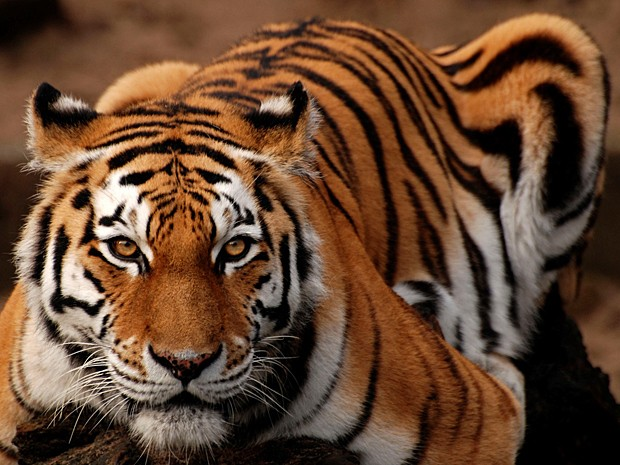
\includegraphics[width=\textwidth]{tigre.jpg} 
        \caption{Tigre} 
        \label{fig:tigre} 
    \end{subfigure} ~ %add desired spacing between images, e. g. ~, \quad, \qquad, \hfill etc. %(or a blank line to force the subfigure onto a new line) 
    \begin{subfigure}[b]{0.317\textwidth} 
        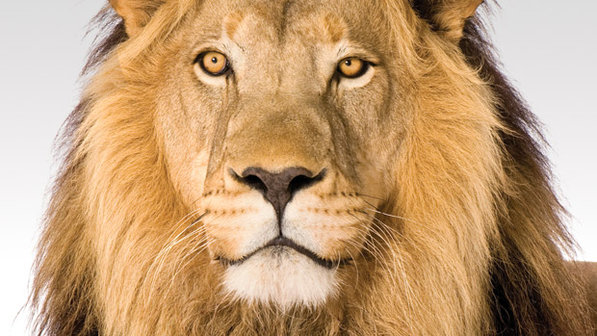
\includegraphics[width=\textwidth]{leao.jpg} 
        \caption{Leão} \label{fig:leao} 
    \end{subfigure} ~ %add desired spacing between images, e. g. ~, \quad, \qquad, \hfill etc. %(or a blank line to force the subfigure onto a new line) 
    \begin{subfigure}[b]{0.317\textwidth} 
        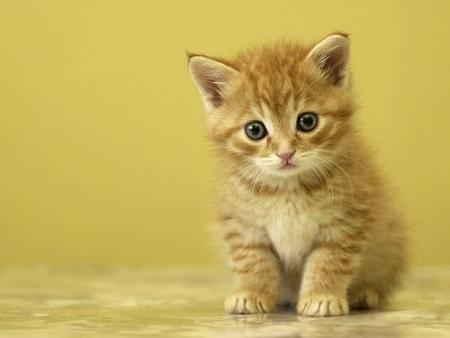
\includegraphics[width=\textwidth]{gato.jpg} 
        \caption{Gato} \label{fig:gato} 
    \end{subfigure}
    \fautor
\end{figure}

A classe \textit{icmc} traz algum comando que auxiliam na inserção da legenda, para utilizá-los basta substituir o \comando{fonte\{\}} por um dos seguintes comando conforme necessário:

\begin{description}

 \item[\comando{fautor}] Insere o texto \aspas{Elaborada pelo autor} como fonte da figura;

 \item[\comando{fadaptada[INF]\{REF\}}] Insere um texto informando que a figura foi adaptada de alguma referência bibliográfica (REF). INF refere-se ao local específico de onde a imagem foi extraída, como por exemplo o número da página. Além disso, INF é um parâmetro opcional e pode receber qualquer cadeia de texto;

 \item[\comando{fdireta[INF]\{REF\}}] Insere um texto informando que a figura próvem diretamente de alguma referência bibliográfica (REF). INF refere-se ao local específico de onde a imagem foi extraída, como por exemplo o número da página. Além disso, INF é um parâmetro opcional e pode receber qualquer cadeia de texto;
 
 \item[\comando{fdadospesquisa}] Insere o texto \aspas{Dados da pesquisa.} como fonte da figura;
 
\end{description}




\section{Tabelas e Quadros}
\label{secao:tabelas_e_quadros}

A inserção de tabelas e quadros é feita de forma semelhante a inserção de figuras, porém são utilizados os ambientes \textit{table} e \textit{quadro}. A principal diferença entre tabelas e quadros, de acordo com \citeonline{NBR14724:2011}, é que as tabelas são destinadas para informações numéricas e os quadros são mais adequados para informações textuais. Em geral, as tabelas devem estar padronizadas conforme o padrão do \citeonline{ibge1993} requerido pelas normas da ABNT para documentos técnicos e acadêmicos.

Como exemplos foram inseridas a \autoref{tab:lista_produtos} que exibe uma de lista de produtos (construída em \LaTeX) e a Tabela \autoref{tabela:populacao_america_sul} que mostra a população dos países da América do Sul (construída segundo o padrão do IBGE). Foi inserido também o \autoref{quadro:editores_texto_livres} com alguns editores que podem ser usados para se trabalhar com \LaTeX para demonstrar a inserção de quadros.

 A lista de tabelas também é um elemento opcional que pode ser incluída com o comando \comando{incluidelistatabelas} antes do início do documento. O mesmo acontece com a lista de quadros que pode ser incluída com o comando \comando{incluidelistaquadros}.

\begin{table}[htb]
\centering
\caption{Lista de produtos}
\label{tab:lista_produtos}
\begin{tabularx}{\textwidth}{X|l|r|r|r} \hline
Produto      & Unidade & Preço (R\$) & Quantidade & Total (R\$) \\ \hline
Arroz        & Kg      & 2,00        & 550        & 1.100,00    \\
Óleo de Soja & L       & 2,50        & 500        & 750,00      \\
Açucar       & Kg      & 3,00        & 100        & 300,00      \\ \hline
\end{tabularx}
\fdadospesquisa
\end{table}

\begin{table}[htb]
\IBGEtab{%
  \caption{População dos países da América do Sul} \label{tabela:populacao_america_sul}
}{%
\begin{tabular}{r|p{6.3cm}|r}        
\toprule
Código  & País            & População   \\ \midrule \midrule
1       & Brasil          & ~~~~~~191.480.630 \\ \midrule 
2       & Argentina       &  39.934.100 \\ \midrule 
3       & Colômbia        &  46.741.100 \\ \midrule 
4       & Paraguai        &   9.694.200 \\ \midrule 
5       & Uruguai         &   3.350.500 \\ \midrule 
6       & Peru            &  28.221.500 \\ \midrule 
7       & Equador         &  13.481.200 \\ \midrule 
8       & Bolívia         &   9.694.200 \\ \midrule 
9       & Venezuela       &  28.121.700 \\ \midrule 
10      & Chile           &  16.803.000 \\ \bottomrule
\end{tabular}
}{%
  \fdireta{wikipedia:2011:america_sul}%
  \nota{Esta é uma nota, que diz que os dados são baseados na
  regressão linear.}%
  \nota[Anotações]{Uma anotação adicional, que pode ser seguida de várias
  outras, porém são opcionais.}%
  }
\end{table}

\begin{quadro}[htb]
\caption{Editores de Texto Livres}
\label{quadro:editores_texto_livres}
\centering
\begin{tabular}{|l|l|r|}        \hline
Editor     & Multiplataforma & Específico para Latex \\ \hline
Kwriter    & Sim             & Não                   \\
Texmaker   & Sim             & Sim                   \\
Kile       & Sim             & Sim                   \\
Geany      & Sim             & Não                   \\ \hline
\end{tabular}
\end{quadro}

\section{Algoritmos e Códigos}
\label{secao:algoritmos_e_codigos}

Além dos corpos flutuantes convencionais para inserir figuras (\comando{begin\{figure\}}) e tabelas (\comando{begin\{table\}}), a classe \textit{icmc} possui mais dois tipos de corpos flutuantes um para algoritmos (\comando{begin\{algoritmo\}}) e outro para códigos-fonte (\comando{begin\{codigo\}}). A utilização de um ou de outro fica a critério do usuário. Como exemplo temos o \autoref{algoritmo:euclidalgoritmo:mdc1} que calcula o máximo divisor comum entre dois números e os Códigos-fonte \ref{codigo:notas_alunos} e \ref{codigo:metodo_leitura} que são uma consulta na \sigla{SQL}{\textit{Structured Query Language}} e uma sobrotina em \textit{Java}.


%\begin{algoritmo}
%\caption{Algoritmo para cálculo de máximo divisor comum MDC($n_1$,$n_2$)}
%\label{algoritmo:mdc1}
%
% \KwIn{Dois números inteiros ($n_1, n_2$)}
% \If(\tcp*[f]{Garante que o maior número seja $n_1$}){$n_2 > n_1$}
%   {troca valores de $n_1$ e $n_2$}
% \Repeat{$r > 0$}{
%    $r \leftarrow$ resto da divisão de $n_1$ por $n_2$
%    $n_1 \leftarrow n_2$
%    $n_2 \leftarrow r$
% }
% \Return $n_1$
%\end{algoritmo}

\begin{codigo}[caption = {Consulta SQL}, label={codigo:notas_alunos},language=SQL, breaklines=true]
SELECT a.nome_aluno AS aluno,
       d.nome_disciplina AS disciplina,
       m.nota AS nota
FROM aluno AS a,
     disciplina AS d,
     matriculado AS m
WHERE a.id_aluno = m.id_aluno
  AND d.id_disciplina = m.id_disciplina
ORDER BY a.nome_aluno, d.nome_disciplina;
\end{codigo}

\begin{codigo}[caption={Subrotina para obter uma entrada do usuário}, label={codigo:metodo_leitura}, language=Java, breaklines=true]
public static String Leitura(){
    BufferedReader reader = new BufferedReader(new InputStreamReader(System.in));
    try {
        return reader.readLine(); // Lê uma linha pelo teclado
    } catch (IOException e) {
        e.printStackTrace();
        return "";
    }
}
\end{codigo}

\begin{algoritmo}
\caption{Algoritmo de Euclides}\label{algoritmo:euclidalgoritmo:mdc1}
\begin{algorithmic}[1]
\Procedure{Euclid}{$a,b$}\Comment{O maior divisor comum de \textit{a} e \textit{b}}
\State $r\gets a\bmod b$
\While{$r\not=0$}\Comment{Tem-se a resposta se \textit{r} é 0}
\State $a\gets b$
\State $b\gets r$
\State $r\gets a\bmod b$
\EndWhile\label{euclidendwhile}
\State \Return $b$\Comment{O maior divisor comum é \textit{b}}
\EndProcedure
\end{algorithmic}
\end{algoritmo}

Existem diversos outros pacotes disponíveis para escrever algoritmos e códigos. Nos exemplos anteriormente foram utilizados o pacote \textit{algorithmicxalgorithm} para definição do ambiente algoritmo e \textit{listings} para a definição do ambiente de código-fonte. O pacote \textit{algorithmicxalgorithm} é usado para escrever algoritmos em alto nível \cite{janos:2005:algpseudocode}. Já o pacote \textit{listings} serve para escrever os códigos em diversas linguagens de programação \cite{moses:2006:listings}.

Caso sejam utilizados os ambientes de algoritmos e código podem ser incluídos os comandos \comando{incluidelistaalgoritmos} e \comando{incluidelistacodigos} antes do \comando{begin\{document\}} para que a lista de algoritmos e a lista de código sejam criadas.


\section{Ambientes Matemáticos}

A classe \textit{icmc} provê os seguintes ambientes matemáticos:
\begin{itemize}
 \item Teoremas (\comando{begin\{teorema\}[\ ]} ... \comando{begin\{teorema\}});
 \item Proposição (\comando{begin\{proposicao\}[\ ]} ... \comando{begin\{proposicao\}});
 \item Lema (\comando{begin\{lema\}[\ ]} ... \comando{begin\{lema\}});
 \item Corolário (\comando{begin\{corolario\}[\ ]} ... \comando{begin\{corolario\}});
 \item Exemplo (\comando{begin\{exemplo\}[\ ]} ... \comando{begin\{exemplo\}});
 \item Observação (\comando{begin\{observacao\}[\ ]} ... \comando{begin\{observacao\}});
 \item Definição (\comando{begin\{definicao\}[\ ]} ... \comando{begin\{definicao\}});
 \item demonstracao (\comando{begin\{demonstracao\}[\ ]} ... \comando{begin\{demonstracao\}}).
\end{itemize}

Abaixo temos um exemplo de proposição com sua demonstração:
\begin{proposicao}
 Sejam $a$ e $b$ reais, tais que $0<a<b$. Então $a^2<b^2$.
\end{proposicao}
\begin{demonstracao}
 Pela hipótese concluímos que $(b+a)>0$ e $(b-a)>0$.

Como $b^2-a^2=(b+a)(b-a)$ concluímos que $b^2-a^2>0$, ou seja, $a^2<b^2$.
\end{demonstracao}

Neste documento tratamos brevemente apenas dos ambientes mencionados anteriormente. Contudo, para escrever expressões matemáticas complexas é preciso estudar uma documentação mais específica como em \citeonline{cassagojr:1997:amslatex}.

Alguns dos ambientes matemáticos da classe \textit{icmc} podem ser usados também para outras finalidades como exemplos e definições.


\section{Definição de outros ambientes}
\label{secao:outros-ambientes}

O classe \textit{icmc} permite a criação de outros ambientes, além dos citados nas seções anteriores, caso seja necessário. Isso é possível graças a extensão da classe \textit{abntex}. O \autoref{codigo:novo-ambiente} deve ser inserido antes do início do documento para criação de um ambiente para gráficos. Para definição de outros ambientes, basta seguir o modelo.


\begin{codigo}[caption={Definição do ambiente \textbf{grafico}}, label={codigo:novo-ambiente}, language=Tex, breaklines=true]
\makeatletter

% Novo list of (listings) para GRÁFICOS --------------------------
\newcommand{\graficoname}{Gráfico}
\newcommand{\graficorefname}{Gráfico}
\newcommand{\listofgraficosname}{Lista de gráficos}

\addto\captionsenglish{% ingles
    %% adjusts names from abnTeX2
    \newcommand{\graficoname}{Graph}
    \newcommand{\graficorefname}{Graph}
    \newcommand{\listofgraficosname}{List of graphs}
}

\newalgoritmo:euclid{grafico}{htbp}{logr}[chapter]
\floatname{grafico}{\graficoname}
\restylefloat{grafico}
\newfloat[chapter]{grafico}{logr}{\graficoname}
\newlistof{listofgraficos}{logr}{\listgraficoname}
\newlistentry{grafico}{logr}{0}

% configurações para atender às regras da ABNT
\renewcommand{\thegrafico}{\thechapter.\@arabic\c@grafico}
\setfloatadjustment{grafico}{\centering}
\renewcommand{\cftgraficoname}{\graficoname\space}
\renewcommand*{\cftgraficoaftersnum}{\hfill\textendash\hfill}
% -----------------------------------------------------------

\makeatother
\end{codigo}

A utilização do novo ambiente no texto segue conforme o \autoref{codigo:usar-novo-ambiente}.

\begin{codigo}[caption={Como usar o ambiente \textbf{grafico}}, label={codigo:usar-novo-ambiente}, language=Tex, breaklines=true]
\begin{grafico}[htb]
\caption{Caption do gráfico}
\label{gra:modelo}
Este é o conteúdo do gráfico.
\end{grafico}
\end{codigo}

Comandos como \comando{autoref\{gra:modelo\}} funcionam normalmente.

Para imprimir a "Lista de gráficos" no documento, insira o \autoref{codigo:lista-novo-ambiente} na classe \textit{icmc}, de modo que ele seja impresso após a "Lista de ilustrações". O código deve ser inserido após a linha 1244.


\begin{codigo}[caption={Código para inserir lista de gráficos}, label={codigo:lista-novo-ambiente}, language=Tex, breaklines=true]
% ---
% inserir lista de gráficos
% ---
\pdfbookmark[0]{\listofgraficosname}{logr}
\listofgraficos*
\cleardoublepage
% ---
\end{codigo}

%\chapter{Listas}
%\label{chapter:listas}
%\section{Abreviaturas e Siglas}

A classe \textit{icmc} implementa a criação da lista de abreviaturas e siglas com o pacote \textit{nomencl}. A inserção de abreviaturas e siglas na lista é realizada com o comando \comando{sigla\{A\}\{B\}} que também insere o conteúdo da sigla no local do documento onde a mesma foi definida. Os parâmetros utilizados são: \textit{A} que é a sigla e \textit{B} que é o nome por extenso. Caso deseja-se inserir a sigla apenas na lista, pode-se utilizar o comando \comando{sigla*\{A\}\{B\}}.

Para se gerar a lista de siglas na parte pre-textual do documento é preciso incluir o comando \comando{incluidelistasiglas} antes do início do documento. Além disto, a compilação do documento deve conter o comando \textit{makeindex} após duas compilações com o \textit{pdflatex}. Por exemplo, supondo que o documento principal tenha o nome de \textit{thesis}, podemos usar a seguinte sequência de comandos:

\begin{verbatim}
pdflatex thesis.tex
pdflatex thesis.tex
makeindex thesis.nlo -s nomencl.ist -o thesis.nls
pdflatex thesis.tex
\end{verbatim}

No \autoref{chapter:ferramentas-uteis} serão apresentadas algumas ferramentas que podem facilitar o processo de compilação do documento. Em especial, o ShareLaTeX não necessita de um processo de compilação especial para gerar a lista de abreviaturas e siglas.


\section{Símbolos}

A definição de símbolos é semelhante a definição de siglas, porém deve ser usado o comando \comando{simbolo\{S\}\{DS\}}, onde \textit{S} é o símbolo e \textit{DS} é a descrição do símbolo. Como exemplo definimos os símbolos $\mathbb{X}$\simbolo{\mathbb{X}}{Variável X} e $\mathsf{I\!R}$\simbolo{\mathsf{I\!R}}{Conjunto dos números reais}. Para incluir a lista de símbolos, basta usar o comando \comando{incluidelistasimbolos} antes do início do documento.


%\chapter{Ferramentas úteis}
%\label{chapter:ferramentas-uteis}
%Existem diversas ferramentas para se trabalhar com \LaTeX. Três ferramentas que merecem destaque são o editor \textit{Texmaker} (\autoref{fig:texmaker}), o ShareLaTeX (\autoref{fig:sharelatex}) e o gerenciador de referências \textit{JabRef} (\autoref{fig:jabref}). Todas as ferramentas são livres e multiplataforma. 

\begin{figure}[htb]
\caption{Tela do Texmaker}
 \label{fig:texmaker}
 \centering
 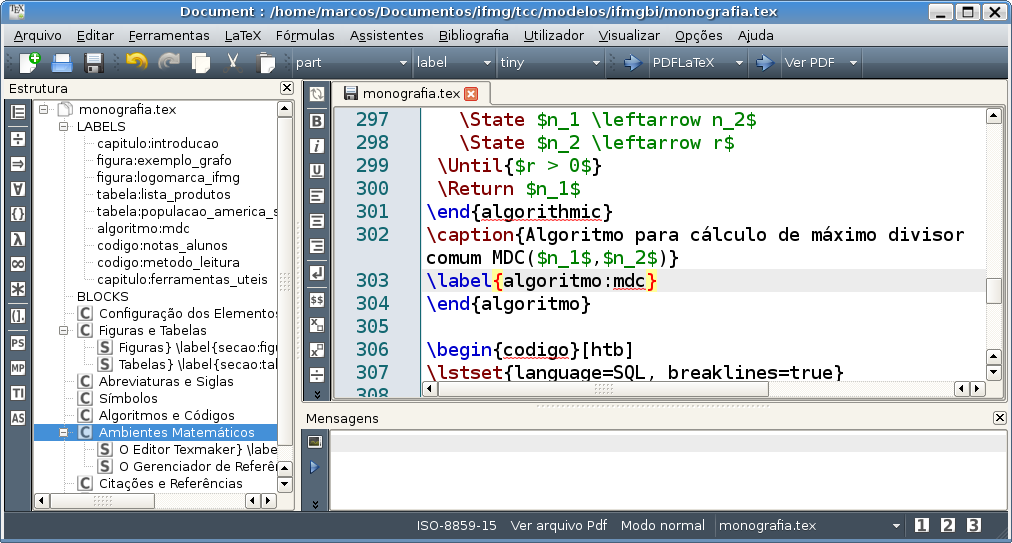
\includegraphics[width=\textwidth]{texmaker.png}
 \fautor
\end{figure}

\begin{figure}[htb]
\caption{Site do ShareLaTeX}
 \label{fig:sharelatex}
 \centering
 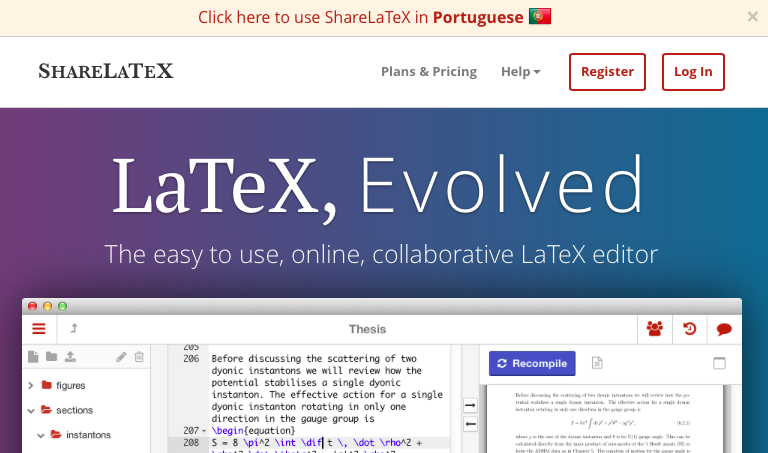
\includegraphics[scale=0.5]{sharelatex.png}
 \fautor
\end{figure}

\begin{figure}[htb]
 \caption{Tela do JabRef}
 \label{fig:jabref}
 \centering
 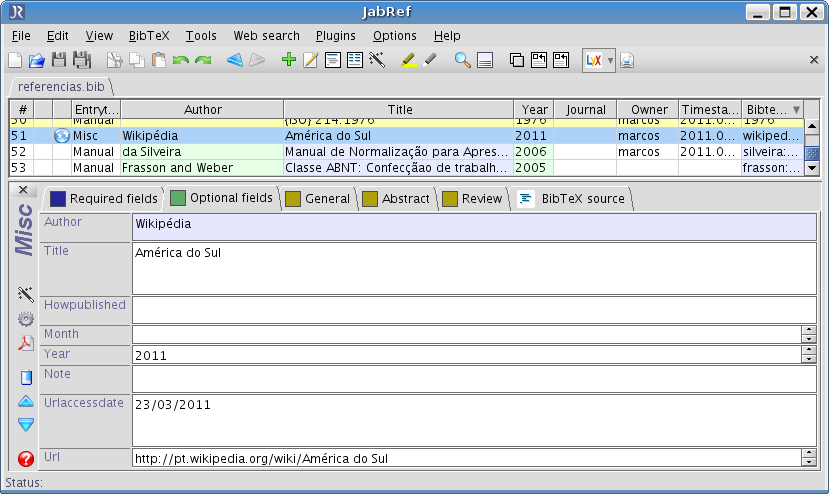
\includegraphics[scale=0.45]{jabref.png}
\fautor
\end{figure}

O Texmaker pode ser obtido em \url{www.xm1math.net/texmaker} e o JabRef pode ser obtido em \url{jabref.sourceforge.ne}. É importante ressaltar que o Texmaker é apenas um editor, para compilar os documentos é necessário um ambiente \LaTeX instalado. Os ambientes Latex mais populares são o Texlive (\url{www.tug.org/texlive}) e o MiKTex (\url{miktex.org}). 

As estrutura de referências do bibtex utilizadas nesse \textit{template} contém alguns parâmetros adicionais que o modelo geral não tem, conforme pode ser consultado em \citeonline{abntex2cite-alf}. Desta forma, recomenda-se fortemente o uso do gerenciador de referências JabRef, uma vez que é possível customizá-lo para atender estas exigências. O código de customização pode ser visto no \autoref{chapter:configuracao-jabref}.

O ShareLaTeX é uma ferramenta de edição de documento em \LaTeX de forma online e está disponível em \url{www.sharelatex.com}. A ferramenta permite o compartilhamento e edição simultânea do conteúdo. Além disso, pode-se consultar o histórico da edições realizadas no documento. A principal vantagem de utilizar o ShareLaTeX é não precisar instalar o compilador para LaTeX.

%\chapter{Citações e referências}
%\label{chapter:citacoes}
%

Em documentos acadêmicos podem existir as citações podem ser: \textbf{implícitas} quando as referências não fazem parte do texto ou \textbf{explícitas} quando o autor referente a citação é mencionado explicitamente na sentença. Nesse sentido, deve-se utilizar os comandos específicos para cada tipo de citação, ou seja, em citações explicitas deve-se usar o comando \comando{citeonline\{\}} e nas demais situações é usado o comando \comando{cite\{\}}. Alguns exemplos são apresentados no \autoref{qua:exemplo-citacao}.

\begin{quadro}[htb]
\caption{Exemplos de citações no documento}
\label{qua:exemplo-citacao}
\centering\small 
\begin{tabular}{|c|c|}        \hline
\textbf{Código em \LaTeX} & \textbf{Código Compilado}\\ \hline\hline
\begin{minipage}[t]{\VerbL}
\vspace{5pt}
\begin{verbatim}
A ironia será assim uma ... proposta
por \citeonline{10520:2000:4.1-1}.
\end{verbatim}
\vspace{5pt}
\end{minipage}
&
\begin{minipage}[t]{\LatL}
\vspace{5pt}
A ironia será assim uma ... proposta 
por \citeonline{10520:2000:4.1-1}.
\vspace{5pt}
\end{minipage}\\\hline

\begin{minipage}[t]{\VerbL}
\vspace{5pt}
\begin{verbatim}
\citeonline[p.~146]{10520:2000:4.2-2}
dizem que ... 
\end{verbatim}
\vspace{5pt}
\end{minipage}
&
\begin{minipage}[t]{\LatL}
\vspace{5pt}
\citeonline[p.~146]{10520:2000:4.2-2} dizem que {...}
\vspace{5pt}
\end{minipage}\\ \hline

\begin{minipage}[t]{\VerbL}
\vspace{5pt}
\begin{verbatim}
``Apesar das ... da filosofia''
\cite[p.~293]{10520:2000:4.1-2}.
\end{verbatim}
\vspace{5pt}
\end{minipage}
&
\begin{minipage}[t]{\LatL}
\vspace{5pt}
``Apesar das {...} da filosofia'' \cite[p.~293]{10520:2000:4.1-2}.
\vspace{5pt}
\end{minipage} \\ \hline

\begin{minipage}[t]{\VerbL}
\vspace{5pt}
\begin{verbatim}
Depois, ...  que prefiro
\cite{10520:2000:4.1-3}.
\end{verbatim}
\vspace{5pt}
\end{minipage}
&
\begin{minipage}[t]{\LatL}
\vspace{5pt}
Depois, {...} que prefiro \cite{10520:2000:4.1-3}.
\vspace{5pt}
\end{minipage}\\ \hline

\end{tabular}
\end{quadro}


Para especificar a página, seção ou capítulo consultado na referência é preciso acrescentá-lo entre colchetes com os comandos \comando{cite[página]\{\}} ou \comando{citeonline[página]\{\}}. O texto colocado entre colchetes aparecerá logo após o ano. Maiores informações sobre os comandos utilizados para citação posem ser consultados no manual de referência da abnTeX2, incluindo o uso de \textbf{apud} \cite{abntex2cite-alf}.


\section{Citações Indiretas}

As citações indiretas são caracterizadas como uma espécie de paráfrase das ideias de um determinado autor, ou seja, o pesquisador, por meio de suas próprias palavras, interpreta o discurso de outrem, contudo, mantendo o mesmo sentido. Outro aspecto que deve ser considerado é a necessidade de o autor (ou os autores) e o ano em que a obra foi publicada serem mencionados. 

Nas citações indiretas há duas formatações possíveis dependendo de como ocorre a citação no texto. Quando o autor é mencionado explicitamente utiliza-se o comando \comando{citeonline\{\}}, caso contrário, deve utilizar o comando \comando{cite\{\}}. 



\section{Citações diretas}
\label{sec-citacao}


As citações diretas ocorrem quando o texto de uma referência é transcrito literalmente. As citações diretas curtas (até três linhas) são inseridas no texto entre aspas duplas. As aspas simples são utilizadas para indicar citação no interior da citação: \aspas{Nas citações, as chamadas pelo sobrenome do autor [...] incluído na sentença devem ser em letras maiúsculas e minúsculas e, quando estiverem entre parênteses, devem ser em letras maiúsculas} \cite[sec.~5]{NBR10520:2002}.

\begin{verbatim}
``Nas citações, as chamadas pelo sobrenome do autor [...] incluído na 
sentença devem ser em letras maiúsculas e minúsculas e, quando 
estiverem entre parênteses, devem ser em letras maiúsculas''
\cite[5]{NBR10520:2002}.
\end{verbatim}

Cabe ressaltar que em \LaTeX as aspas iniciais são diferentes das finais. Para tanto, pode-se utilizar o comando \comando{aspas\{CONTEUDO\}} para inserir um determinado conteúdo entre aspas.

As citações diretas longas (com mais de 3 linhas) podem ser inseridas por meio do ambiente \texttt{citacao}:

\begin{citacao}
As citações diretas, no texto, com mais de três linhas, devem ser
destacadas com recuo de 4 cm da margem esquerda, com letra menor que a do texto
utilizado e sem as aspas. No caso de documentos datilografados, deve-se
observar apenas o recuo \cite[5.3]{NBR10520:2002}.
\end{citacao}

Use o ambiente assim:

\begin{verbatim}
\begin{citacao}
As citações diretas, no texto, com mais de três linhas [...] deve-se 
observar apenas o recuo \cite[5.3]{NBR10520:2002}.
\end{citacao}
\end{verbatim}

O ambiente \texttt{citacao} pode receber como parâmetro opcional um nome de
idioma previamente carregado nas opções da classe (\autoref{sec-hifenizacao}). Nesse
caso, o texto da citação é automaticamente escrito em itálico e a hifenização é
ajustada para o idioma selecionado na opção do ambiente. Por exemplo:

\begin{verbatim}
\begin{citacao}[english]
Text in English language in italic with correct hyphenation.
\end{citacao}
\end{verbatim}

Tem como resultado:

\begin{citacao}[english]
Text in English language in italic with correct hyphenation.
\end{citacao}



% ---
% Finaliza a parte no bookmark do PDF, para que se inicie o bookmark na raiz
% ---
\bookmarksetup{startatroot}% 
% ---

% ----------------------------------------------------------
% ELEMENTOS PÓS-TEXTUAIS
% ----------------------------------------------------------
\postextual

% ----------------------------------------------------------
% Referências bibliográficas
% ----------------------------------------------------------
\bibliography{references}

% ---------------------------------------------------------------------
% GLOSSÁRIO
% ---------------------------------------------------------------------

% Arquivo que contém as definições que vão aparecer no glossário
\newword{WYSIWYG}{``What You See Is What You Get''  ou ``O que você vê é o que você obtém''.  Recurso tem por objetivo permitir que um documento, enquanto manipulado na tela, tenha a mesma aparência de sua utilização, usualmente sendo considerada final. Isso facilita para o desenvolvedor que pode trabalhar visualizando a aparência do documento sem precisar salvar em vários momentos e abrir em um \textit{software} separado de visualização}
\newword{Framework}{é uma abstração que une códigos comuns entre vários projetos de \textit{software} provendo uma funcionalidade genérica. \textit{Frameworks} são projetados com a intenção de facilitar o desenvolvimento de \textit{software}, habilitando designers e programadores a gastarem mais tempo determinando as exigências do \textit{software} do que com detalhes de baixo nível do sistema}

\newword{Template}{é um documento sem conteúdo, com apenas a apresentação visual (apenas cabeçalhos por exemplo) e instruções sobre onde e qual tipo de conteúdo deve entrar a cada parcela da apresentação}

\newword{Padrões de projeto}{ou \textit{Design Pattern}, descreve uma solução geral reutilizável para um problema recorrente no desenvolvimento de sistemas de \textit{software} orientados a objetos. Não é um código final, é uma descrição ou modelo de como resolver o problema do qual trata, que pode ser usada em muitas situações diferentes}

\newword{Web}{Sinônimo mais conhecido de \textit{World Wide Web} (WWW). É a interface gráfica da Internet que torna os serviços disponíveis totalmente transparentes para o usuário e ainda possibilita a manipulação multimídia da informação}

% Comando para incluir todas as definições do arquivo glossario.tex
%\glsaddall
% Impressão do glossário
%\printglossaries

% ----------------------------------------------------------
% Apêndices
% ----------------------------------------------------------

% ---
% Inicia os apêndices
% ---
\begin{apendicesenv}

    \chapter{Complex polynomial's coefficients}
	\label{chapter:poly}
	We present here the coefficients of the polynomial $f(y) = \sum_{k=0}^{6} c_{2k} y^k$ defined in \autoref{eq:poly_f}.

\section{$c_0$}

$$+\frac{x_{1}^{4} x_{2}^{2}}{64} - 0.015625 x_{1}^{4} y_{2}^{2} + \frac{x_{1}^{2} x_{2}^{4}}{64} + \frac{x_{1}^{2} y_{2}^{4}}{64} - 0.015625 x_{2}^{4} y_{1}^{2} + \frac{x_{2}^{2} y_{1}^{4}}{64} + \frac{y_{1}^{2} y_{2}^{2} \left(- y_{1}^{2} + 2 y_{1} y_{2} - y_{2}^{2}\right)}{64}$$
$$+0.09375 x_{1}^{3} x_{2} y_{2}^{2} + 0.03125 x_{1}^{3} \left(- x_{2}^{3} + i y_{2}^{3}\right) + 0.09375 x_{1}^{2} y_{1}^{2} y_{2}^{2} + 0.09375 x_{1} x_{2}^{3} y_{1}^{2} + 0.03125 i x_{2}^{3} y_{1}^{3}$$
$$+\frac{- 6.0 a^{6} \left(x_{1}^{2} x_{2}^{2} y_{2}^{2} + y_{1} \left(x_{1}^{2} x_{2}^{2} y_{1} + y_{2} \left(x_{2}^{2} y_{1}^{2} + y_{2} \left(x_{1}^{2} y_{2} - x_{2}^{2} y_{1}\right)\right)\right)\right) - b^{6} x_{1}^{4} x_{2}^{2} + 2 b^{6} x_{1}^{3} x_{2}^{3} - b^{6} x_{1}^{2} x_{2}^{4}}{64 a^{6}}$$
$$+\frac{0.03125 i a^{6} x_{1} x_{2}^{4} y_{1} + 0.03125 i a^{6} x_{1} y_{1} y_{2}^{4} + 0.015625 b^{6} \left(x_{1}^{4} y_{2}^{2} + x_{2}^{4} y_{1}^{2} + y_{1}^{4} y_{2}^{2} + y_{1}^{2} y_{2}^{4}\right)}{a^{6}}$$
$$+i \left(0.0625 x_{1}^{3} x_{2}^{2} y_{1} + 0.0625 x_{1}^{2} x_{2}^{3} y_{2} + y_{2} \left(0.0625 x_{1} y_{1}^{3} y_{2} + 0.0625 x_{2} y_{1}^{2} y_{2}^{2} + 0.03125 x_{2} \left(x_{1}^{4} + y_{1}^{4}\right)\right)\right)$$
$$+\frac{x_{1} \left(0.046875 b^{4} x_{1}^{3} x_{2}^{2} + 0.046875 b^{4} x_{1} y_{2}^{4} + x_{2} \left(0.125 a^{4} y_{1} y_{2} \left(y_{1}^{2} + y_{2}^{2}\right) + 0.046875 b^{4} x_{1} x_{2}^{3}\right)\right)}{a^{4}}$$
$$+\frac{0.046875 b^{2} \left(a^{2} x_{1}^{4} y_{2}^{2} + a^{2} x_{2}^{4} y_{1}^{2} + a^{2} y_{1}^{4} y_{2}^{2} + a^{2} y_{1}^{2} y_{2}^{4} + b^{2} x_{2}^{2} y_{1}^{4}\right)}{a^{4}}$$
$$+\frac{0.28125 a^{6} x_{1}^{2} x_{2}^{2} y_{1} y_{2} + 0.09375 a^{4} b^{2} x_{1}^{3} x_{2}^{3} + 0.09375 a^{2} b^{4} y_{1}^{3} y_{2}^{3} - 0.015625 b^{6} \left(x_{1}^{2} y_{2}^{4} + x_{2}^{2} y_{1}^{4}\right)}{a^{6}}$$
$$- \frac{0.0625 i a^{6} x_{1} \left(x_{1}^{2} y_{1} y_{2}^{2} + x_{1} x_{2} y_{2}^{3} + x_{2}^{2} y_{1}^{3}\right) + 0.0625 i a^{6} x_{2}^{3} y_{1}^{2} y_{2} + 0.03125 b^{6} y_{1}^{3} y_{2}^{3}}{a^{6}}$$
$$- \frac{0.046875 b^{4} x_{2}^{4} y_{1}^{2} + 0.046875 b^{4} y_{1}^{2} y_{2}^{4} + x_{1} y_{2} \left(0.125 a^{4} x_{2} y_{1} \left(x_{1}^{2} + x_{2}^{2}\right) + 0.046875 b^{4} x_{1}^{3} y_{2}\right)}{a^{4}}$$
$$- \frac{0.09375 i a^{4} x_{1} y_{1}^{2} y_{2}^{3} + 0.046875 b^{2} \left(a^{2} x_{1}^{4} x_{2}^{2} + a^{2} x_{1}^{2} x_{2}^{4} + a^{2} x_{1}^{2} y_{2}^{4} + a^{2} x_{2}^{2} y_{1}^{4} + b^{2} y_{1}^{4} y_{2}^{2}\right)}{a^{4}}$$
$$- \frac{0.28125 a^{4} x_{1} x_{2} y_{1}^{2} y_{2}^{2} + 0.09375 a^{2} b^{2} y_{1}^{3} y_{2}^{3} + 0.09375 x_{2} \left(i a^{4} \left(x_{1}^{3} x_{2} y_{2} + y_{1} \left(x_{1}^{2} x_{2}^{2} + y_{1}^{2} y_{2}^{2}\right)\right) + b^{4} x_{1}^{3} x_{2}^{2}\right)}{a^{4}}$$
$$+\frac{0.09375 b^{4} \left(i a^{2} \left(x_{1}^{3} y_{2}^{3} + x_{2}^{3} y_{1}^{3}\right) + b^{2} x_{1}^{2} x_{2}^{2} y_{1}^{2} + b^{2} x_{1}^{2} x_{2}^{2} y_{2}^{2} + b^{2} x_{1}^{2} y_{1} y_{2}^{3} + b^{2} x_{2}^{2} y_{1}^{3} y_{2}\right)}{a^{6}}$$
$$+\frac{0.28125 \left(a^{2} b^{2} x_{2}^{2} y_{1}^{3} y_{2} + x_{1} \left(a^{2} b^{2} x_{1} y_{1} y_{2}^{3} + x_{2} \left(b^{4} x_{1}^{2} y_{2}^{2} + y_{1} \left(i a^{4} y_{2} \left(x_{1} y_{2} + x_{2} y_{1}\right) + b^{4} x_{2}^{2} y_{1}\right)\right)\right)\right)}{a^{4}}$$
$$+\frac{b^{2} \left(0.28125 a^{2} \left(a^{2} x_{1}^{2} x_{2}^{2} y_{2}^{2} + y_{1}^{2} \left(a^{2} x_{1}^{2} x_{2}^{2} + b^{2} y_{2}^{2} \left(x_{1}^{2} + x_{2}^{2}\right)\right)\right) - 0.03125 i b^{4} x_{1}^{3} y_{2}^{3} - 0.03125 i b^{4} x_{2}^{3} y_{1}^{3}\right)}{a^{6}}$$
$$- \frac{0.09375 b^{2} \left(i a^{4} \left(x_{1}^{3} y_{2}^{3} + x_{2}^{3} y_{1}^{3}\right) + b^{4} x_{1}^{3} x_{2} y_{2}^{2} + b^{4} x_{1}^{2} y_{1}^{2} y_{2}^{2} + b^{4} x_{1} x_{2}^{3} y_{1}^{2} + b^{4} x_{2}^{2} y_{1}^{2} y_{2}^{2}\right)}{a^{6}}$$
$$- \frac{x_{1} \left(a^{2} x_{2} \left(0.28125 b^{2} x_{1}^{2} y_{2}^{2} + y_{1} \left(0.1875 i a^{2} y_{2} \left(x_{1} y_{1} + x_{2} y_{2}\right) + 0.28125 b^{2} x_{2}^{2} y_{1}\right)\right) + 0.28125 b^{4} x_{1} y_{1} y_{2}^{3}\right)}{a^{4}}$$
$$+\frac{b^{2} \left(- 0.28125 a^{2} \left(a^{2} x_{1}^{2} y_{1}^{2} y_{2}^{2} + a^{2} x_{2}^{2} y_{1}^{2} y_{2}^{2} + b^{2} x_{2}^{2} \left(x_{1}^{2} y_{2}^{2} + y_{1}^{2} \left(x_{1}^{2} + y_{1} y_{2}\right)\right)\right) + 0.0625 i b^{4} x_{1} x_{2}^{2} y_{1}^{3}\right)}{a^{6}}$$
$$+\frac{b^{4} \left(0.09375 i a^{2} x_{1} x_{2}^{4} y_{1} + b^{2} y_{2} \left(0.125 x_{1}^{3} x_{2} y_{1} + 0.125 x_{1} x_{2}^{3} y_{1} + 0.0625 i \left(x_{1}^{2} y_{2} \left(x_{1} y_{1} + x_{2} y_{2}\right) + x_{2}^{3} y_{1}^{2}\right)\right)\right)}{a^{6}}$$
$$+\frac{0.09375 i b^{4} \left(b^{2} x_{1}^{3} x_{2}^{2} y_{2} + b^{2} x_{1}^{2} x_{2}^{3} y_{1} + y_{2} \left(a^{2} x_{2} y_{1}^{4} + b^{2} x_{2} y_{1}^{3} y_{2} + x_{1} \left(a^{2} x_{1}^{3} x_{2} + y_{1} y_{2}^{2} \left(a^{2} y_{2} + b^{2} y_{1}\right)\right)\right)\right)}{a^{6}}$$
$$+\frac{0.1875 i b^{2} \left(a^{2} x_{1}^{3} y_{1} y_{2}^{2} + a^{2} x_{1}^{2} x_{2} y_{2}^{3} + b^{2} x_{1}^{3} x_{2}^{2} y_{1} + b^{2} x_{1}^{2} x_{2}^{3} y_{2} + y_{1}^{2} \left(b^{2} x_{2} y_{2}^{3} + x_{1} y_{1} \left(a^{2} x_{2}^{2} + b^{2} y_{2}^{2}\right)\right)\right)}{a^{4}}$$
$$+\frac{b^{2} x_{2} y_{1} y_{2} \left(0.375 a^{2} x_{1}^{3} + 0.375 a^{2} x_{1} x_{2}^{2} + 0.1875 i a^{2} x_{2}^{2} y_{1} + 0.375 b^{2} x_{1} y_{1}^{2} + 0.375 b^{2} x_{1} y_{2}^{2}\right)}{a^{4}}$$
$$+\frac{0.28125 b^{2} \left(i a^{4} \left(x_{1}^{3} x_{2}^{2} y_{2} + y_{1} \left(x_{1}^{2} x_{2}^{3} + y_{1} y_{2}^{2} \left(x_{1} y_{2} + x_{2} y_{1}\right)\right)\right) + b^{4} x_{1} x_{2} y_{1}^{2} y_{2}^{2}\right)}{a^{6}}$$
$$- \frac{b^{2} x_{1} \left(0.03125 i b^{4} x_{1}^{3} x_{2} y_{2} + y_{1} \left(0.03125 i b^{4} y_{2}^{4} - x_{2} \left(0.84375 a^{2} y_{2} \left(a^{2} y_{1} y_{2} + b^{2} x_{1} x_{2}\right) - 0.03125 i b^{4} x_{2}^{3}\right)\right)\right)}{a^{6}}$$
$$- \frac{i b^{6} \left(0.0625 x_{1}^{2} x_{2}^{3} y_{2} + y_{1} \left(0.0625 x_{1}^{3} x_{2}^{2} + y_{1} y_{2} \left(0.0625 x_{2} y_{2}^{2} + y_{1} \left(0.0625 x_{1} y_{2} + 0.03125 x_{2} y_{1}\right)\right)\right)\right)}{a^{6}}$$
$$- \frac{b^{2} x_{1} \left(0.09375 i a^{4} x_{1}^{3} x_{2} y_{2} + y_{1} \left(0.09375 i a^{4} y_{2}^{4} + x_{2} \left(0.09375 i a^{4} x_{2}^{3} + 0.125 b^{4} y_{2} \left(y_{1}^{2} + y_{2}^{2}\right)\right)\right)\right)}{a^{6}}$$
$$- \frac{i b^{2} \left(0.1875 a^{2} x_{2} y_{1}^{2} y_{2}^{3} + 0.1875 b^{2} x_{1}^{2} x_{2} y_{2}^{3} + y_{1}^{3} \left(0.1875 a^{2} x_{1} y_{2}^{2} + x_{2} \left(0.09375 a^{2} y_{1} y_{2} + 0.1875 b^{2} x_{1} x_{2}\right)\right)\right)}{a^{4}}$$
$$- \frac{b^{2} \left(0.375 a^{2} x_{1} x_{2} y_{1}^{3} y_{2} + 0.375 a^{2} x_{1} x_{2} y_{1} y_{2}^{3} + 0.1875 i \left(a^{2} x_{1}^{2} x_{2}^{3} y_{2} + y_{1} \left(b^{2} x_{2}^{3} y_{1} y_{2} + x_{1}^{3} \left(a^{2} x_{2}^{2} + b^{2} y_{2}^{2}\right)\right)\right)\right)}{a^{4}}$$
$$- \frac{b^{4} y_{1} \left(0.28125 i x_{1}^{2} x_{2}^{3} + y_{2} \left(x_{1} \left(0.375 x_{2} \left(x_{1}^{2} + x_{2}^{2}\right) + 0.28125 i y_{1} y_{2}^{2}\right) + 0.28125 i x_{2} y_{1}^{2} y_{2}\right)\right)}{a^{4}}$$
$$+\frac{b^{2} x_{1} x_{2} y_{2} \left(- 0.84375 a^{4} x_{1} x_{2} y_{1} + 0.1875 i b^{4} x_{2} y_{1} y_{2} - b^{2} \left(0.84375 a^{2} y_{1}^{2} y_{2} + 0.28125 x_{1} x_{2} \left(i a^{2} x_{1} + b^{2} y_{1}\right)\right)\right)}{a^{6}}$$
$$+\frac{i b^{2} x_{1} x_{2} y_{1} y_{2} \left(0.5625 a^{4} x_{1} y_{1} + 0.5625 a^{4} x_{2} y_{2} + 0.84375 a^{2} b^{2} x_{1} y_{2} + 0.84375 a^{2} b^{2} x_{2} y_{1} + 0.1875 b^{4} x_{1} y_{1}\right)}{a^{6}}$$
$$- \frac{i b^{2} x_{1} x_{2} y_{1} y_{2} \left(0.84375 a^{4} x_{2} y_{1} + b^{2} \left(0.5625 a^{2} x_{1} y_{1} + 0.5625 a^{2} x_{2} y_{2} + 0.28125 b^{2} \left(x_{1} y_{2} + x_{2} y_{1}\right)\right)\right)}{a^{6}}$$
$$- \frac{0.84375 i b^{2} x_{1}^{2} x_{2} y_{1} y_{2}^{2}}{a^{2}}$$

\section{$c_2$}
$$+0.1875 x_{1}^{3} x_{2}^{3} - 0.09375 x_{1}^{2} x_{2}^{4} + \frac{x_{2}^{4} y_{1}^{2}}{32} + \frac{x_{2}^{2} y_{1}^{4}}{32} + \frac{y_{2}^{2} \left(x_{1}^{4} + x_{1}^{2} y_{2}^{2} + 3 y_{1}^{2} \left(- y_{1}^{2} + 2 y_{1} y_{2} - y_{2}^{2}\right)\right)}{32}$$
$$+x_{1}^{2} \left(x_{2}^{2} \left(- 0.09375 x_{1}^{2} + 0.1875 y_{1}^{2} + 0.1875 y_{2}^{2}\right) + 0.1875 y_{1}^{2} y_{2}^{2}\right) - 0.1875 x_{1} x_{2}^{3} y_{1}^{2} + 0.1875 x_{2}^{2} y_{1}^{2} y_{2}^{2}$$
$$+\frac{- 6.0 a^{6} y_{2} \left(x_{1}^{2} y_{2} \left(x_{1} x_{2} + y_{1} y_{2}\right) + x_{2}^{2} y_{1}^{3}\right) - 3 b^{6} x_{1}^{4} x_{2}^{2} + b^{6} x_{1}^{4} y_{2}^{2} + 6 b^{6} x_{1}^{3} x_{2}^{3} - 3 b^{6} x_{1}^{2} x_{2}^{4} + b^{6} x_{1}^{2} y_{2}^{4}}{32 a^{6}}$$
$$+0.25 i x_{1} y_{1}^{3} y_{2}^{2} + 0.125 i x_{1} y_{1} y_{2}^{4} + 0.125 i x_{2} y_{1}^{4} y_{2} + 0.25 i x_{2} y_{1}^{2} y_{2}^{3} + \frac{0.03125 b^{6} x_{2}^{4} y_{1}^{2}}{a^{6}} + \frac{0.03125 b^{6} x_{2}^{2} y_{1}^{4}}{a^{6}}$$
$$+\frac{0.09375 b^{4} y_{1}^{2} y_{2}^{4} + x_{1} x_{2} \left(0.25 a^{4} y_{1} y_{2} \left(x_{1}^{2} + x_{2}^{2} + y_{1}^{2} + y_{2}^{2}\right) + 0.09375 b^{4} x_{1}^{3} x_{2} + 0.09375 b^{4} x_{1} x_{2}^{3}\right)}{a^{4}}$$
$$+\frac{b^{2} \left(0.09375 a^{2} \left(a^{2} x_{1}^{4} x_{2}^{2} + a^{2} x_{1}^{2} x_{2}^{4} + a^{2} y_{1}^{4} y_{2}^{2} + a^{2} y_{1}^{2} y_{2}^{4} + b^{2} y_{1}^{4} y_{2}^{2}\right) + 0.1875 b^{4} y_{1}^{3} y_{2}^{3}\right)}{a^{6}}$$
$$+\frac{- 0.03125 b^{4} x_{2}^{4} y_{1}^{2} - 0.03125 b^{4} x_{2}^{2} y_{1}^{4} + x_{1}^{2} \left(0.375 i a^{4} x_{2}^{2} \left(x_{1} y_{2} + x_{2} y_{1}\right) - 0.03125 b^{4} x_{1}^{2} y_{2}^{2} - 0.03125 b^{4} y_{2}^{4}\right)}{a^{4}}$$
$$- \frac{0.125 i a^{2} x_{1}^{4} x_{2} y_{2} + 0.25 i a^{2} x_{1}^{3} x_{2}^{2} y_{1} + 0.125 i a^{2} x_{1} x_{2}^{4} y_{1} + 0.03125 b^{2} \left(x_{1}^{2} y_{2}^{2} \left(x_{1}^{2} + y_{2}^{2}\right) + x_{2}^{4} y_{1}^{2} + x_{2}^{2} y_{1}^{4}\right)}{a^{2}}$$
$$- \frac{0.1875 a^{2} b^{4} x_{1}^{3} x_{2}^{3} + 0.1875 a^{2} b^{4} y_{1}^{3} y_{2}^{3} + y_{2} \left(0.25 i a^{6} x_{1}^{2} x_{2}^{3} + 0.09375 b^{6} y_{1}^{4} y_{2} + 0.09375 b^{6} y_{1}^{2} y_{2}^{3}\right)}{a^{6}}$$
$$- 0.5625 x_{1} x_{2} y_{1}^{2} y_{2}^{2} - 0.375 i x_{1} y_{1}^{2} y_{2}^{3} - 0.375 i x_{2} y_{1}^{3} y_{2}^{2} - \frac{0.1875 b^{2} x_{1}^{3} x_{2}^{3}}{a^{2}} - \frac{0.1875 b^{2} y_{1}^{3} y_{2}^{3}}{a^{2}}$$
$$+\frac{x_{1} x_{2} \left(0.1875 a^{2} b^{2} x_{1}^{2} y_{2}^{2} + 0.1875 b^{4} x_{1}^{2} y_{2}^{2} + x_{2} y_{1} \left(- 0.5625 a^{4} x_{1} y_{2} + 0.1875 a^{2} b^{2} x_{2} y_{1} + 0.1875 b^{4} x_{2} y_{1}\right)\right)}{a^{4}}$$
$$+\frac{0.1875 b^{2} \left(b^{4} x_{1}^{2} x_{2}^{2} y_{2}^{2} + b^{4} x_{1}^{2} y_{1}^{2} y_{2}^{2} + y_{1} \left(a^{2} y_{2} \left(a^{2} x_{2}^{2} y_{1}^{2} + b^{2} x_{2}^{2} y_{1}^{2} + x_{1}^{2} y_{2}^{2} \left(a^{2} + b^{2}\right)\right) + b^{4} x_{1}^{2} x_{2}^{2} y_{1}\right)\right)}{a^{6}}$$
$$- \frac{0.1875 b^{4} \left(a^{2} x_{1}^{2} x_{2}^{2} y_{1}^{2} + a^{2} x_{1}^{2} x_{2}^{2} y_{2}^{2} + b^{2} \left(x_{1}^{2} y_{1} y_{2}^{3} + x_{2}^{2} y_{1}^{3} y_{2} + x_{2} \left(x_{1}^{3} y_{2}^{2} + x_{2} y_{1}^{2} \left(x_{1} x_{2} - y_{2}^{2}\right)\right)\right)\right)}{a^{6}}$$
$$- \frac{0.1875 b^{2} \left(a^{2} x_{1}^{2} x_{2}^{2} y_{2}^{2} + a^{2} x_{1}^{2} y_{1}^{2} y_{2}^{2} + a^{2} x_{2}^{2} y_{1}^{2} y_{2}^{2} + y_{1}^{2} \left(a^{2} x_{1}^{2} x_{2}^{2} + b^{2} y_{2}^{2} \left(x_{1}^{2} + x_{2}^{2}\right)\right)\right)}{a^{4}}$$
$$+\frac{0.125 i b^{2} \left(a^{4} x_{1}^{4} x_{2} y_{2} + a^{2} b^{2} x_{1}^{4} x_{2} y_{2} + y_{1} \left(b^{4} x_{2} y_{1}^{3} y_{2} + x_{1} \left(a^{4} x_{2}^{4} + b^{2} \left(a^{2} x_{2}^{4} + b^{2} y_{2}^{4}\right)\right)\right)\right)}{a^{6}}$$
$$+\frac{0.25 i b^{2} \left(a^{4} x_{1}^{2} x_{2}^{3} y_{2} + a^{2} b^{2} x_{1}^{2} x_{2}^{3} y_{2} + y_{1} \left(a^{4} x_{1}^{3} x_{2}^{2} + b^{2} \left(a^{2} x_{1}^{3} x_{2}^{2} + b^{2} y_{1} y_{2}^{2} \left(x_{1} y_{1} + x_{2} y_{2}\right)\right)\right)\right)}{a^{6}}$$
$$+\frac{b^{2} y_{1} y_{2} \left(0.375 i a^{2} b^{2} x_{2} y_{1}^{2} y_{2} + x_{1} \left(0.375 i a^{4} y_{1} y_{2}^{2} + b^{2} \left(0.375 i a^{2} y_{1} y_{2}^{2} + 0.25 b^{2} x_{2} \left(x_{1}^{2} + x_{2}^{2} + y_{1}^{2} + y_{2}^{2}\right)\right)\right)\right)}{a^{6}}$$
$$+\frac{b^{2} x_{2} \left(0.5625 a^{4} x_{1} y_{1}^{2} y_{2}^{2} + 0.5625 a^{2} b^{2} x_{1} y_{1}^{2} y_{2}^{2} + 0.375 i \left(b^{4} x_{1}^{3} x_{2} y_{2} + y_{1} \left(a^{4} y_{1}^{2} y_{2}^{2} + b^{4} x_{1}^{2} x_{2}^{2}\right)\right)\right)}{a^{6}}$$
$$- \frac{b^{2} x_{1} \left(0.125 i b^{4} x_{1}^{3} x_{2} y_{2} + y_{1} \left(0.125 i a^{4} y_{2}^{4} + 0.125 i a^{2} b^{2} y_{2}^{4} - x_{2}^{2} \left(0.5625 a^{2} x_{1} y_{2} \left(a^{2} + b^{2}\right) - 0.125 i b^{4} x_{2}^{2}\right)\right)\right)}{a^{6}}$$
$$- \frac{i b^{2} y_{1}^{2} y_{2} \left(0.25 a^{2} x_{2} y_{2}^{2} + 0.25 b^{2} x_{2} y_{2}^{2} + y_{1} \left(0.25 a^{2} x_{1} y_{2} + 0.25 b^{2} x_{1} y_{2} + 0.125 x_{2} y_{1} \left(a^{2} + b^{2}\right)\right)\right)}{a^{4}}$$
$$- \frac{0.25 b^{2} x_{1} x_{2} \left(a^{4} y_{1}^{3} y_{2} + a^{4} y_{1} y_{2}^{3} + a^{2} b^{2} x_{2}^{2} y_{1} y_{2} + a^{2} b^{2} y_{1}^{3} y_{2} + b^{2} \left(a^{2} y_{1} y_{2}^{3} + i b^{2} x_{1} x_{2} \left(x_{1} y_{1} + x_{2} y_{2}\right)\right)\right)}{a^{6}}$$
$$- \frac{b^{2} y_{1} \left(0.375 i a^{2} b^{2} x_{1}^{2} x_{2}^{3} + y_{2} \left(0.375 i b^{4} x_{2} y_{1}^{2} y_{2} + x_{1} \left(0.25 a^{2} x_{2} \left(a^{2} x_{1}^{2} + a^{2} x_{2}^{2} + b^{2} x_{1}^{2}\right) + 0.375 i b^{4} y_{1} y_{2}^{2}\right)\right)\right)}{a^{6}}$$
$$- \frac{b^{2} x_{1} x_{2} \left(0.375 i a^{2} x_{1} x_{2} \left(a^{2} x_{1} y_{2} + a^{2} x_{2} y_{1} + b^{2} x_{1} y_{2}\right) + 0.5625 b^{4} x_{1} x_{2} y_{1} y_{2} + 0.5625 b^{4} y_{1}^{2} y_{2}^{2}\right)}{a^{6}}$$

\section{$c_4$}
$$+0.234375 x_{1}^{4} x_{2}^{2} + 0.234375 x_{1}^{2} x_{2}^{4} - 0.015625 x_{1}^{2} y_{2}^{4} + \frac{x_{2}^{4} y_{1}^{2}}{64} + \frac{y_{2}^{2} \left(x_{1}^{4} + 15 y_{1}^{2} \left(- y_{1}^{2} + 2 y_{1} y_{2} - y_{2}^{2}\right)\right)}{64}$$
$$+0.09375 x_{1}^{2} x_{2}^{2} y_{1}^{2} + 0.09375 x_{1}^{2} y_{1} y_{2}^{3} + 0.09375 x_{2}^{2} y_{1}^{3} y_{2} - x_{2}^{2} \left(0.46875 x_{1}^{3} x_{2} + 0.015625 y_{1}^{4}\right)$$
$$- 0.09375 x_{1}^{3} x_{2} y_{2}^{2} - 0.09375 x_{1}^{2} y_{1}^{2} y_{2}^{2} - 0.09375 x_{1}^{2} y_{2}^{2} \left(i x_{1} y_{2} - x_{2}^{2}\right) - 0.09375 x_{1} x_{2}^{3} y_{1}^{2} - 0.09375 i x_{2}^{3} y_{1}^{3}$$
$$+\frac{8.0 a^{6} x_{1} x_{2}^{3} y_{1} y_{2} + b^{6} x_{1}^{2} y_{2}^{4} + b^{6} x_{2}^{2} y_{1}^{4} + x_{2}^{2} \left(- 6.0 a^{6} y_{1}^{2} y_{2}^{2} - 15 b^{6} x_{1}^{4} + 30 b^{6} x_{1}^{3} x_{2} - 15.0 b^{6} x_{1}^{2} x_{2}^{2}\right)}{64 a^{6}}$$
$$+\frac{0.046875 a^{2} b^{2} x_{1}^{4} x_{2}^{2} + 0.046875 a^{2} b^{2} x_{1}^{2} x_{2}^{4} + y_{1} y_{2} \left(0.125 a^{4} x_{1}^{3} x_{2} + 0.046875 b^{4} y_{1}^{3} y_{2} + 0.046875 b^{4} y_{1} y_{2}^{3}\right)}{a^{4}}$$
$$+\frac{0.1875 i a^{4} x_{1}^{3} y_{1} y_{2}^{2} + 0.1875 i a^{4} x_{1} x_{2} \left(x_{1} y_{2}^{3} + x_{2} y_{1}^{3}\right) + 0.09375 a^{2} b^{2} y_{1}^{3} y_{2}^{3} + 0.09375 b^{4} x_{1}^{3} x_{2}^{3}}{a^{4}}$$
$$+i \left(0.15625 x_{1}^{4} x_{2} y_{2} + 0.3125 x_{1} y_{1}^{3} y_{2}^{2} + 0.15625 x_{2} y_{1}^{4} y_{2} + y_{1} \left(0.15625 x_{1} y_{2}^{4} + x_{2}^{3} \left(0.15625 x_{1} x_{2} + 0.1875 y_{1} y_{2}\right)\right)\right)$$
$$+\frac{a^{4} x_{2} \left(0.28125 x_{1} y_{1}^{2} y_{2}^{2} + 0.3125 i \left(x_{1}^{2} x_{2}^{2} y_{2} + y_{1} \left(x_{1}^{3} x_{2} + y_{1} y_{2}^{3}\right)\right)\right) + 0.203125 b^{4} x_{1}^{2} y_{2}^{4} + 0.203125 b^{4} x_{2}^{2} y_{1}^{4}}{a^{4}}$$
$$+\frac{b^{2} \left(0.203125 a^{4} \left(x_{1}^{4} y_{2}^{2} + x_{2}^{4} y_{1}^{2}\right) - 0.015625 b^{4} x_{1}^{4} y_{2}^{2} + 0.234375 b^{4} y_{1}^{4} y_{2}^{2} + 0.234375 b^{4} y_{1}^{2} y_{2}^{4}\right)}{a^{6}}$$
$$- \frac{x_{2} \left(0.046875 a^{2} b^{4} x_{1}^{4} x_{2} + 0.046875 a^{2} b^{4} x_{1}^{2} x_{2}^{3} + y_{1} \left(0.125 a^{6} x_{1} y_{2} \left(y_{1}^{2} + y_{2}^{2}\right) + 0.015625 b^{6} x_{2}^{3} y_{1}\right)\right)}{a^{6}}$$
$$- \frac{0.28125 a^{4} x_{1}^{2} x_{2}^{2} y_{1} y_{2} + b^{2} \left(0.09375 a^{2} x_{1}^{3} x_{2}^{3} + y_{1}^{2} y_{2}^{2} \left(0.046875 a^{2} \left(y_{1}^{2} + y_{2}^{2}\right) + 0.09375 b^{2} y_{1} y_{2}\right)\right)}{a^{4}}$$
$$- \frac{0.46875 i a^{4} x_{1} y_{1}^{2} y_{2}^{3} + 0.46875 i a^{4} x_{2} y_{1}^{3} y_{2}^{2} + 0.203125 b^{2} \left(a^{2} x_{1}^{2} y_{2}^{4} + a^{2} x_{2}^{2} y_{1}^{4} + b^{2} \left(x_{1}^{4} y_{2}^{2} + x_{2}^{4} y_{1}^{2}\right)\right)}{a^{4}}$$
$$+\frac{- 0.46875 i a^{6} x_{1}^{2} x_{2}^{2} \left(x_{1} y_{2} + x_{2} y_{1}\right) + 0.09375 i b^{6} x_{1}^{3} y_{2}^{3} + 0.09375 i b^{6} x_{2}^{3} y_{1}^{3} - 0.46875 b^{6} y_{1}^{3} y_{2}^{3}}{a^{6}}$$
$$+\frac{b^{4} \left(0.21875 i a^{2} x_{1}^{3} y_{2}^{3} + 0.21875 i a^{2} x_{2}^{3} y_{1}^{3} + 0.09375 b^{2} \left(x_{1} \left(x_{1} y_{1}^{2} y_{2}^{2} + x_{2} \left(x_{1}^{2} y_{2}^{2} + x_{2}^{2} y_{1}^{2}\right)\right) + x_{2}^{2} y_{1}^{2} y_{2}^{2}\right)\right)}{a^{6}}$$
$$+\frac{0.21875 b^{2} \left(a^{2} x_{2}^{2} y_{1}^{3} y_{2} + b^{2} x_{1}^{2} y_{1}^{2} y_{2}^{2} + b^{2} x_{2}^{2} y_{1}^{2} y_{2}^{2} + x_{1} \left(a^{2} x_{1} y_{1} y_{2}^{3} + b^{2} x_{2} \left(x_{1}^{2} y_{2}^{2} + x_{2}^{2} y_{1}^{2}\right)\right)\right)}{a^{4}}$$
$$+\frac{x_{1} \left(a^{4} x_{2} \left(0.5625 i a^{2} x_{1} y_{1}^{2} y_{2} + x_{2} \left(0.5625 i a^{2} y_{1} y_{2}^{2} + 0.21875 b^{2} x_{1} \left(y_{1}^{2} + y_{2}^{2}\right)\right)\right) - 0.09375 b^{6} x_{1} y_{1} y_{2}^{3}\right)}{a^{6}}$$
$$- \frac{b^{2} \left(0.21875 i a^{4} x_{1}^{3} y_{2}^{3} + 0.21875 i a^{4} x_{2}^{3} y_{1}^{3} + 0.09375 b^{4} x_{2}^{2} \left(x_{1}^{2} y_{2}^{2} + y_{1}^{2} \left(x_{1}^{2} + y_{1} y_{2}\right)\right)\right)}{a^{6}}$$
$$- \frac{0.21875 b^{2} \left(b^{2} x_{1}^{2} x_{2}^{2} y_{1}^{2} + b^{2} x_{1}^{2} x_{2}^{2} y_{2}^{2} + b^{2} x_{2}^{2} y_{1}^{3} y_{2} + x_{1} \left(a^{2} x_{2} \left(x_{1}^{2} y_{2}^{2} + x_{2}^{2} y_{1}^{2}\right) + b^{2} x_{1} y_{1} y_{2}^{3}\right)\right)}{a^{4}}$$
$$+\frac{y_{1} \left(0.03125 i b^{2} x_{1} x_{2}^{4} - y_{2} \left(0.84375 i a^{2} x_{1}^{2} x_{2} y_{2} + y_{1} \left(0.84375 i a^{2} x_{1} x_{2}^{2} + 0.21875 b^{2} y_{2} \left(x_{1}^{2} + x_{2}^{2}\right)\right)\right)\right)}{a^{2}}$$
$$+\frac{i b^{2} \left(0.0625 x_{1}^{3} x_{2}^{2} y_{1} + y_{2} \left(0.0625 x_{1} y_{1}^{3} y_{2} + 0.03125 x_{1} \left(x_{1}^{3} x_{2} + y_{1} y_{2}^{3}\right) + 0.03125 x_{2} y_{1}^{4} + 0.0625 x_{2} y_{1}^{2} y_{2}^{2}\right)\right)}{a^{2}}$$
$$+\frac{b^{2} x_{1} y_{2} \left(0.09375 i a^{2} b^{2} y_{1}^{2} y_{2}^{2} + x_{2} \left(0.0625 i a^{4} x_{1} x_{2}^{2} + 0.125 b^{4} y_{1}^{3} + 0.125 b^{4} y_{1} y_{2}^{2}\right)\right)}{a^{6}}$$
$$+\frac{b^{2} x_{2} \left(0.375 a^{2} x_{1} y_{1}^{3} y_{2} + 0.375 a^{2} x_{1} y_{1} y_{2}^{3} + 0.375 b^{2} x_{1} x_{2}^{2} y_{1} y_{2} + 0.09375 i b^{2} \left(x_{1}^{3} x_{2} y_{2} + y_{1} \left(x_{1}^{2} x_{2}^{2} + y_{1}^{2} y_{2}^{2}\right)\right)\right)}{a^{4}}$$
$$+\frac{b^{2} x_{1} \left(0.4375 i a^{2} x_{1}^{2} y_{1} y_{2}^{2} + x_{2} \left(0.4375 i a^{2} x_{1} y_{2}^{3} + y_{1} \left(0.4375 i a^{2} x_{2} y_{1}^{2} + 0.375 b^{2} x_{1}^{2} y_{2}\right)\right)\right)}{a^{4}}$$
$$+\frac{b^{2} x_{2} y_{1} y_{2} \left(0.34375 a^{4} x_{1}^{2} x_{2} + 0.34375 a^{2} b^{2} x_{1} y_{1} y_{2} + x_{2} \left(0.4375 i a^{4} x_{2} y_{1} + 0.28125 b^{4} x_{1}^{2}\right)\right)}{a^{6}}$$
$$+\frac{i b^{4} \left(- 0.03125 a^{2} x_{1} x_{2}^{4} y_{1} - 0.03125 a^{2} x_{1} y_{1} y_{2}^{4} + 0.46875 b^{2} \left(x_{1}^{3} x_{2}^{2} y_{2} + y_{1} \left(x_{1}^{2} x_{2}^{3} + y_{1} y_{2}^{2} \left(x_{1} y_{2} + x_{2} y_{1}\right)\right)\right)\right)}{a^{6}}$$
$$- \frac{i b^{4} \left(0.0625 x_{1}^{3} x_{2}^{2} y_{1} + 0.0625 x_{1}^{2} x_{2}^{3} y_{2} + y_{2} \left(0.0625 x_{1} y_{1}^{3} y_{2} + 0.0625 x_{2} y_{1}^{2} y_{2}^{2} + 0.03125 x_{2} \left(x_{1}^{4} + y_{1}^{4}\right)\right)\right)}{a^{4}}$$
$$- \frac{b^{2} y_{1} \left(0.09375 i a^{4} x_{1}^{2} x_{2}^{3} + y_{2} \left(0.09375 i a^{4} x_{2} y_{1}^{2} y_{2} + x_{1} \left(0.09375 i a^{4} y_{1} y_{2}^{2} + 0.125 b^{4} x_{2} \left(x_{1}^{2} + x_{2}^{2}\right)\right)\right)\right)}{a^{6}}$$
$$- \frac{i b^{2} x_{1} \left(0.1875 b^{4} x_{1}^{2} y_{1} y_{2}^{2} + x_{2} \left(0.1875 b^{4} x_{1} y_{2}^{3} + x_{2} \left(0.09375 a^{4} x_{1}^{2} y_{2} + 0.1875 b^{4} y_{1}^{3}\right)\right)\right)}{a^{6}}$$
$$- \frac{b^{2} x_{2} y_{1} y_{2} \left(0.375 a^{4} x_{1}^{3} + 0.375 a^{4} x_{1} x_{2}^{2} + b^{2} \left(0.375 a^{2} x_{1} y_{1}^{2} + 0.375 a^{2} x_{1} y_{2}^{2} + 0.1875 i b^{2} x_{2}^{2} y_{1}\right)\right)}{a^{6}}$$
$$- \frac{i b^{6} \left(0.3125 x_{1} y_{1}^{3} y_{2}^{2} + 0.15625 x_{1} \left(x_{1}^{3} x_{2} y_{2} + y_{1} \left(x_{2}^{4} + y_{2}^{4}\right)\right) + 0.15625 x_{2} y_{1}^{4} y_{2} + 0.3125 x_{2} y_{1}^{2} y_{2}^{3}\right)}{a^{6}}$$
$$- \frac{i b^{4} x_{1} \left(0.4375 a^{2} x_{1}^{2} y_{1} y_{2}^{2} + x_{2} \left(0.4375 a^{2} x_{1} y_{2}^{3} + x_{2} \left(0.4375 a^{2} y_{1}^{3} + 0.3125 b^{2} x_{1} \left(x_{1} y_{1} + x_{2} y_{2}\right)\right)\right)\right)}{a^{6}}$$
$$- \frac{b^{2} x_{2} y_{1} y_{2} \left(0.34375 a^{2} b^{2} x_{1}^{2} x_{2} + y_{1} \left(0.34375 a^{4} x_{1} y_{2} + b^{2} \left(0.4375 i a^{2} x_{2}^{2} + 0.28125 b^{2} x_{1} y_{2}\right)\right)\right)}{a^{6}}$$
$$+\frac{i b^{2} x_{1} x_{2} y_{1} y_{2} \left(a^{2} \left(0.03125 a^{2} \left(x_{1} y_{2} + x_{2} y_{1}\right) + 0.6875 b^{2} x_{1} y_{1} + 0.6875 b^{2} x_{2} y_{2}\right) + 0.84375 b^{4} x_{2} y_{1}\right)}{a^{6}}$$
$$+\frac{i b^{4} x_{1} x_{2} y_{1} y_{2} \left(- 0.03125 a^{2} x_{1} y_{2} - 0.03125 a^{2} x_{2} y_{1} - 0.5625 b^{2} x_{1} y_{1} + 0.84375 b^{2} x_{1} y_{2} - 0.5625 b^{2} x_{2} y_{2}\right)}{a^{6}}$$
$$- \frac{0.6875 i b^{2} x_{1} x_{2} y_{1} y_{2} \left(x_{1} y_{1} + x_{2} y_{2}\right)}{a^{2}}$$

\section{$c_6$}

$$- 0.0625 x_{1}^{4} y_{2}^{2} + 0.625 x_{1}^{3} x_{2}^{3} - 0.0625 x_{1}^{2} y_{2}^{4} - 0.0625 x_{2}^{4} y_{1}^{2} - 0.0625 x_{2}^{2} y_{1}^{4} - \frac{5 y_{1}^{2} y_{2}^{2} \left(y_{1}^{2} - 2 y_{1} y_{2} + y_{2}^{2}\right)}{16}$$
$$+x_{1} \left(0.375 x_{1} y_{1} y_{2}^{3} + x_{2} \left(0.375 x_{1}^{2} y_{2}^{2} - x_{2} \left(0.3125 x_{1} \left(x_{1}^{2} + x_{2}^{2}\right) - 0.375 x_{2} y_{1}^{2}\right)\right)\right) + 0.375 x_{2}^{2} y_{1}^{3} y_{2}$$
$$+\frac{- 6.0 a^{6} \left(x_{1}^{2} \left(x_{2}^{2} \left(y_{1}^{2} + y_{2}^{2}\right) + y_{1}^{2} y_{2}^{2}\right) + x_{2}^{2} y_{1}^{2} y_{2}^{2}\right) + 64.0 a^{4} b^{4} x_{1}^{2} y_{2}^{2} - 5 b^{6} x_{1}^{4} x_{2}^{2} + 10 b^{6} x_{1}^{3} x_{2}^{3} - 5 b^{6} x_{1}^{2} x_{2}^{4}}{16 a^{6}}$$
$$+\frac{b^{2} \left(a^{2} \left(0.375 a^{2} x_{1}^{3} x_{2}^{3} + 0.375 a^{2} y_{1}^{3} y_{2}^{3} + b^{2} \left(x_{2}^{2} \left(4.0 a^{2} y_{1}^{2} + 0.375 x_{1}^{3} x_{2}\right) + 0.375 y_{1}^{3} y_{2}^{3}\right)\right) + 0.625 b^{4} y_{1}^{3} y_{2}^{3}\right)}{a^{6}}$$
$$- \frac{0.0625 b^{6} x_{2}^{4} y_{1}^{2} + 0.0625 b^{6} x_{2}^{2} y_{1}^{4} + x_{1} y_{2} \left(- 1.125 a^{6} x_{2} y_{1} \left(x_{1} x_{2} + y_{1} y_{2}\right) + 0.0625 b^{6} x_{1}^{3} y_{2} + 0.0625 b^{6} x_{1} y_{2}^{3}\right)}{a^{6}}$$
$$- \frac{0.1875 b^{4} y_{1}^{2} y_{2}^{4} + x_{1} x_{2} \left(0.5 a^{4} y_{1} y_{2} \left(x_{1}^{2} + x_{2}^{2} + y_{1}^{2} + y_{2}^{2}\right) + 0.1875 b^{4} x_{1}^{3} x_{2} + 0.1875 b^{4} x_{1} x_{2}^{3}\right)}{a^{4}}$$
$$- \frac{b^{2} \left(0.1875 a^{2} \left(a^{2} x_{1}^{4} x_{2}^{2} + a^{2} x_{1}^{2} x_{2}^{4} + a^{2} y_{1}^{4} y_{2}^{2} + a^{2} y_{1}^{2} y_{2}^{4} + b^{2} y_{1}^{4} y_{2}^{2}\right) + 0.3125 b^{4} y_{1}^{4} y_{2}^{2} + 0.3125 b^{4} y_{1}^{2} y_{2}^{4}\right)}{a^{6}}$$
$$- \frac{0.4375 b^{2} \left(a^{2} x_{1}^{4} y_{2}^{2} + a^{2} x_{1}^{2} y_{2}^{4} + a^{2} x_{2}^{4} y_{1}^{2} + a^{2} x_{2}^{2} y_{1}^{4} + b^{2} \left(x_{1}^{2} y_{2}^{2} \left(x_{1}^{2} + y_{2}^{2}\right) + x_{2}^{4} y_{1}^{2} + x_{2}^{2} y_{1}^{4}\right)\right)}{a^{4}}$$
$$+\frac{b^{2} \left(0.625 a^{4} x_{1} x_{2}^{3} y_{1}^{2} + b^{2} \left(0.625 a^{2} x_{1} x_{2}^{3} y_{1}^{2} + 0.375 b^{2} \left(x_{1} \left(x_{1} y_{1} y_{2}^{3} + x_{2} \left(x_{1}^{2} y_{2}^{2} + x_{2}^{2} y_{1}^{2}\right)\right) + x_{2}^{2} y_{1}^{3} y_{2}\right)\right)\right)}{a^{6}}$$
$$+\frac{b^{2} \left(0.625 a^{2} y_{2} \left(a^{2} x_{2}^{2} y_{1}^{3} + b^{2} x_{2}^{2} y_{1}^{3} + x_{1}^{2} y_{2} \left(a^{2} y_{1} y_{2} + b^{2} y_{1} y_{2} + x_{1} x_{2} \left(a^{2} + b^{2}\right)\right)\right) - 0.375 b^{4} x_{1}^{2} x_{2}^{2} y_{1}^{2}\right)}{a^{6}}$$
$$- \frac{b^{4} \left(0.625 a^{2} x_{1}^{2} x_{2}^{2} y_{1}^{2} + 0.625 a^{2} x_{1}^{2} x_{2}^{2} y_{2}^{2} + 0.625 a^{2} x_{1}^{2} y_{1}^{2} y_{2}^{2} + 0.375 b^{2} y_{2}^{2} \left(x_{1}^{2} \left(x_{2}^{2} + y_{1}^{2}\right) + x_{2}^{2} y_{1}^{2}\right)\right)}{a^{6}}$$
$$+\frac{b^{2} \left(- 0.625 a^{2} x_{1}^{2} y_{1}^{2} y_{2}^{2} - 0.625 a^{2} x_{2}^{2} y_{1}^{2} y_{2}^{2} + 0.5 b^{2} x_{1} x_{2} y_{1} y_{2}^{3} - 0.625 x_{2}^{2} \left(a^{2} x_{1}^{2} y_{2}^{2} + y_{1}^{2} \left(a^{2} x_{1}^{2} + b^{2} y_{2}^{2}\right)\right)\right)}{a^{4}}$$
$$+\frac{b^{2} x_{1} x_{2} y_{1} y_{2} \left(0.5 a^{2} \left(a^{2} x_{1}^{2} + a^{2} x_{2}^{2} + a^{2} y_{1}^{2} + a^{2} y_{2}^{2} + b^{2} x_{1}^{2} + b^{2} x_{2}^{2} + b^{2} y_{1}^{2}\right) + 1.125 b^{4} x_{1} x_{2} + 1.125 b^{4} y_{1} y_{2}\right)}{a^{6}}$$
$$- \frac{b^{2} x_{1} x_{2} y_{1} y_{2} \left(0.125 a^{2} \left(a^{2} x_{1} x_{2} + b^{2} x_{1} x_{2} + y_{1} y_{2} \left(a^{2} + b^{2}\right)\right) + 0.5 b^{4} x_{1}^{2} + 0.5 b^{4} x_{2}^{2} + 0.5 b^{4} y_{1}^{2} + 0.5 b^{4} y_{2}^{2}\right)}{a^{6}}$$
$$- \frac{8.0 b^{4} x_{1} x_{2} y_{1} y_{2}}{a^{2}}$$


\section{$c_8$}

$$+0.234375 x_{1}^{4} x_{2}^{2} + 0.234375 x_{1}^{2} x_{2}^{4} - 0.015625 x_{1}^{2} y_{2}^{4} + \frac{x_{2}^{4} y_{1}^{2}}{64} + \frac{y_{2}^{2} \left(x_{1}^{4} + 15 y_{1}^{2} \left(- y_{1}^{2} + 2 y_{1} y_{2} - y_{2}^{2}\right)\right)}{64}$$
$$+0.09375 i x_{1}^{3} y_{2}^{3} + 0.09375 x_{1}^{2} y_{1} y_{2}^{3} + 0.09375 i x_{2}^{3} y_{1}^{3} + 0.09375 x_{2}^{2} y_{1}^{3} y_{2} - x_{2}^{2} \left(0.46875 x_{1}^{3} x_{2} + 0.015625 y_{1}^{4}\right)$$
$$- \frac{6.0 a^{6} \left(x_{1} \left(x_{1} y_{1}^{2} y_{2}^{2} + x_{2} \left(x_{1}^{2} y_{2}^{2} - x_{2} \left(x_{1} \left(y_{1}^{2} + y_{2}^{2}\right) - x_{2} y_{1}^{2}\right)\right)\right) + x_{2}^{2} y_{1}^{2} y_{2}^{2}\right) + 15 b^{6} x_{1}^{4} x_{2}^{2} + 15 b^{6} x_{1}^{2} x_{2}^{4}}{64 a^{6}}$$
$$+\frac{4.0 a^{6} x_{1}^{3} x_{2} y_{1} y_{2} + 4.0 a^{6} x_{1} x_{2}^{3} y_{1} y_{2} + 1.5 a^{2} b^{4} y_{1}^{2} y_{2}^{4} + b^{6} \left(x_{1}^{2} \left(15 x_{1} x_{2}^{3} + 0.5 y_{2}^{4}\right) + 0.5 x_{2}^{2} y_{1}^{4}\right)}{32 a^{6}}$$
$$+\frac{b^{2} \left(0.046875 a^{2} x_{1}^{4} x_{2}^{2} + 0.046875 a^{2} x_{1}^{2} x_{2}^{4} + 0.09375 a^{2} y_{1}^{3} y_{2}^{3} + 0.09375 b^{2} x_{1}^{3} x_{2}^{3} + 0.046875 b^{2} y_{1}^{4} y_{2}^{2}\right)}{a^{4}}$$
$$+\frac{0.28125 a^{4} x_{1} x_{2} y_{1}^{2} y_{2}^{2} + 0.203125 a^{2} b^{2} x_{1}^{4} y_{2}^{2} + 0.203125 b^{4} x_{1}^{2} y_{2}^{4} + 0.203125 b^{4} x_{2}^{2} y_{1}^{4}}{a^{4}}$$
$$+\frac{y_{1}^{2} \left(0.46875 i a^{6} x_{1} y_{2}^{3} + 0.46875 i a^{6} x_{2} y_{1} y_{2}^{2} + b^{2} \left(0.203125 a^{4} x_{2}^{4} + 0.234375 b^{4} y_{1}^{2} y_{2}^{2} + 0.234375 b^{4} y_{2}^{4}\right)\right)}{a^{6}}$$
$$+\frac{- 0.125 a^{6} x_{1} x_{2} y_{1} y_{2}^{3} - 0.015625 b^{6} x_{2}^{4} y_{1}^{2} + x_{1}^{2} \left(0.46875 i a^{6} x_{2}^{2} \left(x_{1} y_{2} + x_{2} y_{1}\right) - 0.015625 b^{6} x_{1}^{2} y_{2}^{2}\right)}{a^{6}}$$
$$- \frac{0.046875 a^{2} b^{2} y_{1}^{4} y_{2}^{2} + 0.046875 a^{2} b^{2} y_{1}^{2} y_{2}^{4} + x_{1} x_{2} \left(0.125 a^{4} y_{1}^{3} y_{2} + 0.046875 b^{4} x_{1}^{3} x_{2} + 0.046875 b^{4} x_{1} x_{2}^{3}\right)}{a^{4}}$$
$$- \frac{0.1875 i a^{4} x_{1}^{3} y_{1} y_{2}^{2} + 0.1875 i a^{4} x_{1} x_{2} \left(x_{1} y_{2}^{3} + x_{2} y_{1}^{3}\right) + 0.09375 a^{2} b^{2} x_{1}^{3} x_{2}^{3} + 0.09375 b^{4} y_{1}^{3} y_{2}^{3}}{a^{4}}$$
$$- i \left(0.15625 x_{1}^{4} x_{2} y_{2} + 0.15625 x_{2} y_{1}^{4} y_{2} + y_{1} \left(0.15625 x_{1} y_{2}^{4} + x_{2}^{3} \left(0.15625 x_{1} x_{2} + 0.1875 y_{1} y_{2}\right)\right)\right)$$
$$- \frac{a^{4} \left(0.28125 x_{1}^{2} x_{2}^{2} y_{1} y_{2} + 0.3125 i \left(x_{1}^{2} x_{2}^{3} y_{2} + y_{1} \left(x_{1}^{3} x_{2}^{2} + y_{1} y_{2}^{2} \left(x_{1} y_{1} + x_{2} y_{2}\right)\right)\right)\right) + 0.203125 b^{4} x_{1}^{4} y_{2}^{2}}{a^{4}}$$
$$+\frac{b^{2} \left(- 0.203125 a^{2} \left(a^{2} x_{1}^{2} y_{2}^{4} + a^{2} x_{2}^{2} y_{1}^{4} + b^{2} x_{2}^{4} y_{1}^{2}\right) + 0.09375 b^{4} x_{1} x_{2}^{3} y_{1}^{2} - 0.46875 b^{4} y_{1}^{3} y_{2}^{3}\right)}{a^{6}}$$
$$+\frac{b^{2} \left(0.21875 i a^{4} x_{2}^{3} y_{1}^{3} + y_{2}^{2} \left(0.21875 i a^{4} x_{1}^{3} y_{2} + 0.09375 b^{4} \left(x_{1}^{2} \left(x_{1} x_{2} + y_{1}^{2}\right) + x_{2}^{2} y_{1}^{2}\right)\right)\right)}{a^{6}}$$
$$+\frac{0.21875 b^{2} \left(a^{2} x_{2}^{2} y_{1}^{3} y_{2} + b^{2} x_{1}^{2} y_{1}^{2} y_{2}^{2} + b^{2} x_{2}^{2} y_{1}^{2} y_{2}^{2} + x_{1} \left(a^{2} x_{1} y_{1} y_{2}^{3} + b^{2} x_{2} \left(x_{1}^{2} y_{2}^{2} + x_{2}^{2} y_{1}^{2}\right)\right)\right)}{a^{4}}$$
$$+\frac{x_{1} \left(a^{4} x_{2} \left(0.84375 i a^{2} x_{1} y_{1} y_{2}^{2} + x_{2} \left(0.84375 i a^{2} y_{1}^{2} y_{2} + 0.21875 b^{2} x_{1} \left(y_{1}^{2} + y_{2}^{2}\right)\right)\right) - 0.09375 i b^{6} x_{1}^{2} y_{2}^{3}\right)}{a^{6}}$$
$$- \frac{b^{4} \left(0.21875 i a^{2} x_{1}^{3} y_{2}^{3} + 0.09375 b^{2} \left(x_{1}^{2} x_{2}^{2} y_{2}^{2} + y_{1} \left(x_{1}^{2} x_{2}^{2} y_{1} + x_{1}^{2} y_{2}^{3} + i x_{2}^{3} y_{1}^{2} + x_{2}^{2} y_{1}^{2} y_{2}\right)\right)\right)}{a^{6}}$$
$$- \frac{0.21875 b^{2} \left(b^{2} x_{1}^{2} x_{2}^{2} y_{1}^{2} + b^{2} x_{1}^{2} x_{2}^{2} y_{2}^{2} + b^{2} x_{1}^{2} y_{1} y_{2}^{3} + b^{2} x_{2}^{2} y_{1}^{3} y_{2} + x_{2} \left(a^{2} x_{1}^{3} y_{2}^{2} + x_{2}^{2} y_{1}^{2} \left(a^{2} x_{1} + i b^{2} y_{1}\right)\right)\right)}{a^{4}}$$
$$+\frac{y_{1} \left(- a^{2} y_{2} \left(0.5625 i a^{2} x_{1}^{2} x_{2} y_{1} + y_{2} \left(0.5625 i a^{2} x_{1} x_{2}^{2} + 0.21875 b^{2} y_{1} \left(x_{1}^{2} + x_{2}^{2}\right)\right)\right) + 0.03125 i b^{4} x_{1} x_{2}^{4}\right)}{a^{4}}$$
$$+\frac{i b^{4} \left(0.0625 x_{1}^{3} x_{2}^{2} y_{1} + y_{2} \left(0.0625 x_{1} y_{1}^{3} y_{2} + 0.03125 x_{1} \left(x_{1}^{3} x_{2} + y_{1} y_{2}^{3}\right) + 0.03125 x_{2} y_{1}^{4} + 0.0625 x_{2} y_{1}^{2} y_{2}^{2}\right)\right)}{a^{4}}$$
$$+\frac{b^{2} y_{2} \left(0.09375 i a^{4} x_{2} y_{1}^{3} y_{2} + x_{1} \left(0.09375 i a^{4} y_{1}^{2} y_{2}^{2} + b^{2} x_{2} \left(0.0625 i a^{2} x_{1} x_{2}^{2} + 0.125 b^{2} y_{1}^{3} + 0.125 b^{2} y_{1} y_{2}^{2}\right)\right)\right)}{a^{6}}$$
$$+\frac{i b^{2} x_{1} \left(0.1875 b^{4} x_{1}^{2} y_{1} y_{2}^{2} + x_{2} \left(0.1875 b^{4} x_{1} y_{2}^{3} + x_{2} \left(0.09375 a^{4} x_{1} \left(x_{1} y_{2} + x_{2} y_{1}\right) + 0.1875 b^{4} y_{1}^{3}\right)\right)\right)}{a^{6}}$$
$$+\frac{b^{2} x_{2} y_{1} y_{2} \left(0.375 a^{4} x_{1} y_{1}^{2} + 0.375 a^{4} x_{1} y_{2}^{2} + 0.375 a^{2} b^{2} x_{1}^{3} + 0.375 a^{2} b^{2} x_{1} x_{2}^{2} + 0.1875 i b^{4} x_{2}^{2} y_{1}\right)}{a^{6}}$$
$$+\frac{i b^{6} \left(0.3125 x_{1} y_{1}^{3} y_{2}^{2} + 0.15625 x_{1} \left(x_{1}^{3} x_{2} y_{2} + y_{1} \left(x_{2}^{4} + y_{2}^{4}\right)\right) + 0.15625 x_{2} y_{1}^{4} y_{2} + 0.3125 x_{2} y_{1}^{2} y_{2}^{3}\right)}{a^{6}}$$
$$+\frac{i b^{4} x_{1} \left(0.4375 a^{2} x_{1}^{2} y_{1} y_{2}^{2} + x_{2} \left(0.4375 a^{2} x_{1} y_{2}^{3} + x_{2} \left(0.4375 a^{2} y_{1}^{3} + 0.3125 b^{2} x_{1} \left(x_{1} y_{1} + x_{2} y_{2}\right)\right)\right)\right)}{a^{6}}$$
$$+\frac{b^{2} x_{2} y_{1} y_{2} \left(0.34375 a^{4} x_{1}^{2} x_{2} + b^{2} \left(0.34375 a^{2} x_{1} y_{1} y_{2} + x_{2} \left(0.4375 i a^{2} x_{2} y_{1} + 0.28125 b^{2} x_{1}^{2}\right)\right)\right)}{a^{6}}$$
$$- \frac{i b^{2} \left(0.0625 x_{1} y_{1}^{3} y_{2}^{2} + 0.03125 x_{1} \left(x_{1}^{3} x_{2} y_{2} + y_{1} \left(x_{2}^{4} + y_{2}^{4}\right)\right) + 0.03125 x_{2} y_{1}^{4} y_{2} + 0.0625 x_{2} y_{1}^{2} y_{2}^{3}\right)}{a^{2}}$$
$$- \frac{b^{2} x_{1} \left(0.09375 i a^{2} b^{2} y_{1}^{2} y_{2}^{3} + x_{2} \left(0.125 b^{4} x_{1}^{2} y_{1} y_{2} + x_{2} \left(0.0625 i a^{4} x_{1} \left(x_{1} y_{1} + x_{2} y_{2}\right) + 0.125 b^{4} x_{2} y_{1} y_{2}\right)\right)\right)}{a^{6}}$$
$$- \frac{b^{2} x_{2} \left(0.375 a^{2} x_{1} x_{2}^{2} y_{1} y_{2} + b^{2} \left(0.375 x_{1} y_{1}^{3} y_{2} + 0.375 x_{1} y_{1} y_{2}^{3} + 0.09375 i \left(x_{1}^{3} x_{2} y_{2} + y_{1} \left(x_{1}^{2} x_{2}^{2} + y_{1}^{2} y_{2}^{2}\right)\right)\right)\right)}{a^{4}}$$
$$- \frac{b^{2} \left(x_{1} \left(0.4375 i x_{1}^{2} y_{1} y_{2}^{2} + x_{2} \left(0.4375 i x_{1} y_{2}^{3} + y_{1} \left(0.375 x_{1}^{2} y_{2} + 0.4375 i x_{2} y_{1}^{2}\right)\right)\right) + 0.4375 i x_{2}^{3} y_{1}^{2} y_{2}\right)}{a^{2}}$$
$$- \frac{b^{2} x_{1} y_{1} y_{2} \left(0.46875 i b^{4} y_{1} y_{2}^{2} + x_{2} \left(0.34375 a^{2} b^{2} x_{1} x_{2} + y_{1} y_{2} \left(0.34375 a^{4} + 0.28125 b^{4}\right)\right)\right)}{a^{6}}$$
$$+\frac{i b^{4} x_{2} \left(0.03125 a^{2} x_{1}^{2} y_{1} y_{2}^{2} + 0.03125 a^{2} x_{1} x_{2} y_{1}^{2} y_{2} - 0.46875 b^{2} \left(x_{1}^{3} x_{2} y_{2} + y_{1} \left(x_{1}^{2} x_{2}^{2} + y_{1}^{2} y_{2}^{2}\right)\right)\right)}{a^{6}}$$
$$+\frac{i b^{2} x_{1} x_{2} y_{1} y_{2} \left(0.6875 a^{4} x_{1} y_{1} - 0.03125 a^{4} x_{1} y_{2} - 0.03125 a^{4} x_{2} y_{1} + 0.6875 a^{4} x_{2} y_{2} + 0.5625 b^{4} \left(x_{1} y_{1} + x_{2} y_{2}\right)\right)}{a^{6}}$$
$$- \frac{i b^{4} x_{1} x_{2} y_{1} y_{2} \left(0.6875 a^{2} \left(x_{1} y_{1} + x_{2} y_{2}\right) + 0.84375 b^{2} x_{1} y_{2} + 0.84375 b^{2} x_{2} y_{1}\right)}{a^{6}}$$

\section{$c_{10}$}

$$+0.1875 x_{1}^{3} x_{2}^{3} - 0.09375 x_{1}^{2} x_{2}^{4} + \frac{x_{2}^{4} y_{1}^{2}}{32} + \frac{x_{2}^{2} y_{1}^{4}}{32} + \frac{y_{2}^{2} \left(x_{1}^{4} + x_{1}^{2} y_{2}^{2} + 3 y_{1}^{2} \left(- y_{1}^{2} + 2 y_{1} y_{2} - y_{2}^{2}\right)\right)}{32}$$
$$+x_{1}^{2} \left(x_{2}^{2} \left(- 0.09375 x_{1}^{2} + 0.1875 y_{1}^{2} + 0.1875 y_{2}^{2}\right) + 0.1875 y_{1}^{2} y_{2}^{2}\right) - 0.1875 x_{1} x_{2}^{3} y_{1}^{2} + 0.1875 x_{2}^{2} y_{1}^{2} y_{2}^{2}$$
$$+\frac{- 6.0 a^{6} y_{2} \left(x_{1}^{2} y_{2} \left(x_{1} x_{2} + y_{1} y_{2}\right) + x_{2}^{2} y_{1}^{3}\right) - 3 b^{6} x_{1}^{4} x_{2}^{2} + b^{6} x_{1}^{4} y_{2}^{2} + 6 b^{6} x_{1}^{3} x_{2}^{3} - 3 b^{6} x_{1}^{2} x_{2}^{4} + b^{6} x_{1}^{2} y_{2}^{4}}{32 a^{6}}$$
$$+\frac{x_{2} \left(0.125 i a^{6} x_{1}^{4} y_{2} + 0.25 i a^{6} x_{1}^{3} x_{2} y_{1} + 0.25 i a^{6} x_{1}^{2} x_{2}^{2} y_{2} + x_{2} y_{1} \left(0.125 i a^{6} x_{1} x_{2}^{2} + 0.03125 b^{6} y_{1} \left(x_{2}^{2} + y_{1}^{2}\right)\right)\right)}{a^{6}}$$
$$+\frac{0.09375 b^{4} y_{1}^{2} y_{2}^{4} + x_{1} x_{2} \left(0.25 a^{4} y_{1} y_{2} \left(x_{1}^{2} + x_{2}^{2} + y_{1}^{2} + y_{2}^{2}\right) + 0.09375 b^{4} x_{1}^{3} x_{2} + 0.09375 b^{4} x_{1} x_{2}^{3}\right)}{a^{4}}$$
$$+\frac{b^{2} \left(0.09375 a^{2} \left(a^{2} x_{1}^{4} x_{2}^{2} + a^{2} x_{1}^{2} x_{2}^{4} + a^{2} y_{1}^{4} y_{2}^{2} + a^{2} y_{1}^{2} y_{2}^{4} + b^{2} y_{1}^{4} y_{2}^{2}\right) + 0.1875 b^{4} y_{1}^{3} y_{2}^{3}\right)}{a^{6}}$$
$$+\frac{- 0.03125 b^{4} x_{2}^{4} y_{1}^{2} - 0.03125 b^{4} x_{2}^{2} y_{1}^{4} + y_{2}^{2} \left(0.375 i a^{4} y_{1}^{2} \left(x_{1} y_{2} + x_{2} y_{1}\right) - 0.03125 b^{4} x_{1}^{4} - 0.03125 b^{4} x_{1}^{2} y_{2}^{2}\right)}{a^{4}}$$
$$- \frac{0.25 i a^{2} x_{1} y_{1}^{3} y_{2}^{2} + 0.125 i a^{2} x_{1} y_{1} y_{2}^{4} + 0.125 i a^{2} x_{2} y_{1}^{4} y_{2} + 0.03125 b^{2} \left(x_{1}^{2} y_{2}^{2} \left(x_{1}^{2} + y_{2}^{2}\right) + x_{2}^{4} y_{1}^{2} + x_{2}^{2} y_{1}^{4}\right)}{a^{2}}$$
$$- \frac{0.1875 a^{2} b^{4} x_{1}^{3} x_{2}^{3} + 0.1875 a^{2} b^{4} y_{1}^{3} y_{2}^{3} + y_{1}^{2} y_{2}^{2} \left(0.09375 b^{6} y_{1}^{2} + y_{2} \left(0.25 i a^{6} x_{2} + 0.09375 b^{6} y_{2}\right)\right)}{a^{6}}$$
$$- 0.375 i x_{1}^{3} x_{2}^{2} y_{2} - 0.375 i x_{1}^{2} x_{2}^{3} y_{1} - 0.5625 x_{1} x_{2} y_{1}^{2} y_{2}^{2} - \frac{0.1875 b^{2} x_{1}^{3} x_{2}^{3}}{a^{2}} - \frac{0.1875 b^{2} y_{1}^{3} y_{2}^{3}}{a^{2}}$$
$$+\frac{x_{1} x_{2} \left(0.1875 a^{2} b^{2} x_{1}^{2} y_{2}^{2} + 0.1875 b^{4} x_{1}^{2} y_{2}^{2} + x_{2} y_{1} \left(- 0.5625 a^{4} x_{1} y_{2} + 0.1875 a^{2} b^{2} x_{2} y_{1} + 0.1875 b^{4} x_{2} y_{1}\right)\right)}{a^{4}}$$
$$+\frac{0.1875 b^{2} \left(b^{4} x_{1}^{2} x_{2}^{2} y_{2}^{2} + b^{4} x_{1}^{2} y_{1}^{2} y_{2}^{2} + y_{1} \left(a^{2} y_{2} \left(a^{2} x_{2}^{2} y_{1}^{2} + b^{2} x_{2}^{2} y_{1}^{2} + x_{1}^{2} y_{2}^{2} \left(a^{2} + b^{2}\right)\right) + b^{4} x_{1}^{2} x_{2}^{2} y_{1}\right)\right)}{a^{6}}$$
$$- \frac{0.1875 b^{4} \left(a^{2} x_{1}^{2} x_{2}^{2} y_{1}^{2} + a^{2} x_{1}^{2} x_{2}^{2} y_{2}^{2} + b^{2} \left(x_{1}^{2} y_{1} y_{2}^{3} + x_{2}^{2} y_{1}^{3} y_{2} + x_{2} \left(x_{1}^{3} y_{2}^{2} + x_{2} y_{1}^{2} \left(x_{1} x_{2} - y_{2}^{2}\right)\right)\right)\right)}{a^{6}}$$
$$- \frac{0.1875 b^{2} \left(a^{2} x_{1}^{2} x_{2}^{2} y_{2}^{2} + a^{2} x_{1}^{2} y_{1}^{2} y_{2}^{2} + a^{2} x_{2}^{2} y_{1}^{2} y_{2}^{2} + y_{1}^{2} \left(a^{2} x_{1}^{2} x_{2}^{2} + b^{2} y_{2}^{2} \left(x_{1}^{2} + x_{2}^{2}\right)\right)\right)}{a^{4}}$$
$$+\frac{0.125 i b^{2} \left(a^{4} x_{2} y_{1}^{4} y_{2} + a^{2} b^{2} x_{2} y_{1}^{4} y_{2} + x_{1} \left(b^{4} x_{1}^{3} x_{2} y_{2} + y_{1} \left(a^{4} y_{2}^{4} + b^{2} \left(a^{2} y_{2}^{4} + b^{2} x_{2}^{4}\right)\right)\right)\right)}{a^{6}}$$
$$+\frac{0.25 b^{2} \left(b^{4} x_{1} x_{2} y_{1} y_{2}^{3} + i \left(b^{4} x_{1}^{2} x_{2}^{3} y_{2} + y_{1} \left(a^{2} y_{1} y_{2}^{2} \left(a^{2} x_{2} y_{2} + b^{2} x_{2} y_{2} + x_{1} y_{1} \left(a^{2} + b^{2}\right)\right) + b^{4} x_{1}^{3} x_{2}^{2}\right)\right)\right)}{a^{6}}$$
$$+\frac{b^{4} y_{1} \left(0.375 i a^{2} x_{1}^{2} x_{2}^{3} + b^{2} y_{2} \left(x_{1} \left(0.25 x_{2} \left(x_{1}^{2} + x_{2}^{2} + y_{1}^{2}\right) + 0.375 i y_{1} y_{2}^{2}\right) + 0.375 i x_{2} y_{1}^{2} y_{2}\right)\right)}{a^{6}}$$
$$+\frac{b^{2} x_{1} x_{2} \left(0.5625 a^{2} y_{1}^{2} y_{2}^{2} + 0.5625 b^{2} x_{1} x_{2} y_{1} y_{2} + 0.5625 b^{2} y_{1}^{2} y_{2}^{2} + 0.375 i x_{1} x_{2} \left(a^{2} x_{1} y_{2} + a^{2} x_{2} y_{1} + b^{2} x_{1} y_{2}\right)\right)}{a^{4}}$$
$$- \frac{b^{2} y_{1} \left(0.125 i b^{4} x_{2} y_{1}^{3} y_{2} + x_{1} \left(0.125 i a^{4} x_{2}^{4} + 0.125 i a^{2} b^{2} x_{2}^{4} - y_{2} \left(0.5625 a^{4} x_{1} x_{2}^{2} - 0.125 i b^{4} y_{2}^{3}\right)\right)\right)}{a^{6}}$$
$$- \frac{i b^{2} \left(0.25 a^{2} b^{2} x_{1}^{3} x_{2}^{2} y_{1} + y_{2} \left(0.25 b^{4} x_{2} y_{1}^{2} y_{2}^{2} + x_{1} \left(0.125 a^{2} x_{1}^{3} x_{2} \left(a^{2} + b^{2}\right) + 0.25 b^{4} y_{1}^{3} y_{2}\right)\right)\right)}{a^{6}}$$
$$- \frac{0.25 b^{2} x_{1} x_{2} \left(a^{2} y_{1}^{3} y_{2} + a^{2} y_{1} y_{2}^{3} + b^{2} x_{2}^{2} y_{1} y_{2} + b^{2} y_{1}^{3} y_{2} + b^{2} y_{1} y_{2}^{3} + i x_{1} x_{2} \left(a^{2} x_{1} y_{1} + a^{2} x_{2} y_{2} + b^{2} x_{2} y_{2}\right)\right)}{a^{4}}$$
$$- \frac{b^{2} y_{1} y_{2} \left(0.375 i b^{2} x_{2} y_{1}^{2} y_{2} + x_{1} \left(0.375 i a^{2} y_{1} y_{2}^{2} + 0.375 i b^{2} y_{1} y_{2}^{2} + 0.25 x_{2} \left(a^{2} x_{1}^{2} + a^{2} x_{2}^{2} + b^{2} x_{1}^{2}\right)\right)\right)}{a^{4}}$$
$$- \frac{b^{2} x_{2} \left(0.5625 b^{4} x_{1}^{2} x_{2} y_{1} y_{2} + 0.5625 b^{4} x_{1} y_{1}^{2} y_{2}^{2} + 0.375 i \left(b^{4} x_{1}^{3} x_{2} y_{2} + y_{1} \left(a^{4} y_{1}^{2} y_{2}^{2} + b^{4} x_{1}^{2} x_{2}^{2}\right)\right)\right)}{a^{6}}$$

\section{$c_{12}$}

$$+\frac{x_{1}^{4} x_{2}^{2}}{64} - 0.015625 x_{1}^{4} y_{2}^{2} + \frac{x_{1}^{2} x_{2}^{4}}{64} + \frac{x_{1}^{2} y_{2}^{4}}{64} - 0.015625 x_{2}^{4} y_{1}^{2} + \frac{x_{2}^{2} y_{1}^{4}}{64} + \frac{y_{1}^{2} y_{2}^{2} \left(- y_{1}^{2} + 2 y_{1} y_{2} - y_{2}^{2}\right)}{64}$$
$$+x_{1} \left(0.09375 x_{1} y_{1}^{2} y_{2}^{2} + x_{2} \left(0.09375 x_{1}^{2} y_{2}^{2} + x_{2}^{2} \left(- 0.03125 x_{1}^{2} + 0.09375 y_{1}^{2}\right)\right)\right) + 0.09375 x_{2}^{2} y_{1}^{2} y_{2}^{2}$$
$$- \frac{a^{6} \left(6.0 x_{1}^{2} x_{2}^{2} y_{1}^{2} + 6.0 x_{1}^{2} x_{2}^{2} y_{2}^{2} + 6.0 x_{1}^{2} y_{1} y_{2}^{3} + 6.0 x_{2}^{2} y_{1}^{3} y_{2} + 2.0 i \left(x_{1}^{3} y_{2}^{3} + x_{2}^{3} y_{1}^{3}\right)\right) + b^{6} x_{1}^{2} x_{2}^{4}}{64 a^{6}}$$
$$+\frac{4.0 i a^{6} x_{1}^{2} x_{2} y_{2}^{3} + 4.0 i a^{6} x_{1} x_{2}^{2} y_{1}^{3} + b^{6} \left(x_{1}^{3} \left(x_{1} y_{2}^{2} + x_{2}^{2} \left(- x_{1} + 2 x_{2}\right)\right) + x_{2}^{4} y_{1}^{2} + y_{1}^{4} y_{2}^{2} + y_{1}^{2} y_{2}^{4}\right)}{64 a^{6}}$$
$$+\frac{a^{4} y_{1} y_{2} \left(0.125 x_{1} x_{2} y_{1}^{2} + 0.125 x_{1} x_{2} y_{2}^{2} + 0.0625 i \left(x_{1}^{3} y_{2} + x_{2}^{3} y_{1}\right)\right) + 0.046875 b^{4} x_{1}^{2} x_{2}^{4} + 0.046875 b^{4} x_{1}^{2} y_{2}^{4}}{a^{4}}$$
$$+\frac{0.09375 i a^{4} x_{1} y_{1}^{2} y_{2}^{3} + 0.046875 b^{2} \left(a^{2} x_{1}^{4} y_{2}^{2} + a^{2} x_{2}^{4} y_{1}^{2} + a^{2} y_{1}^{4} y_{2}^{2} + a^{2} y_{1}^{2} y_{2}^{4} + b^{2} x_{2}^{2} \left(x_{1}^{4} + y_{1}^{4}\right)\right)}{a^{4}}$$
$$+\frac{0.09375 \left(i a^{4} x_{2} \left(x_{1}^{3} x_{2} y_{2} + y_{1} \left(x_{1}^{2} x_{2}^{2} + y_{1}^{2} y_{2}^{2}\right)\right) + a^{2} b^{2} x_{1}^{3} x_{2}^{3} + b^{4} y_{1}^{3} y_{2}^{3}\right)}{a^{4}}$$
$$+0.28125 x_{1}^{2} x_{2}^{2} y_{1} y_{2} - 0.03125 i x_{1} x_{2}^{4} y_{1} - 0.03125 i x_{1} y_{1} y_{2}^{4} - \frac{0.015625 b^{6} x_{1}^{2} y_{2}^{4}}{a^{6}} - \frac{0.015625 b^{6} x_{2}^{2} y_{1}^{4}}{a^{6}}$$
$$- 0.03125 i x_{1}^{4} x_{2} y_{2} - 0.0625 i x_{1} y_{1}^{3} y_{2}^{2} - 0.03125 i x_{2} y_{1}^{4} y_{2} - 0.0625 i x_{2} y_{1}^{2} y_{2}^{3} - \frac{0.03125 b^{6} y_{1}^{3} y_{2}^{3}}{a^{6}}$$
$$- \frac{x_{1} \left(a^{4} x_{2} \left(0.125 x_{1}^{2} y_{1} y_{2} + x_{2} \left(0.0625 i x_{1} \left(x_{1} y_{1} + x_{2} y_{2}\right) + 0.125 x_{2} y_{1} y_{2}\right)\right) + 0.046875 b^{4} x_{1}^{3} y_{2}^{2}\right)}{a^{4}}$$
$$- \frac{0.046875 b^{2} \left(a^{2} x_{1}^{4} x_{2}^{2} + a^{2} x_{1}^{2} x_{2}^{4} + a^{2} x_{1}^{2} y_{2}^{4} + a^{2} x_{2}^{2} y_{1}^{4} + b^{2} y_{1}^{2} \left(x_{2}^{4} + y_{1}^{2} y_{2}^{2} + y_{2}^{4}\right)\right)}{a^{4}}$$
$$+\frac{- 0.28125 a^{6} x_{1} x_{2} y_{1}^{2} y_{2}^{2} - 0.09375 a^{4} b^{2} y_{1}^{3} y_{2}^{3} - 0.09375 a^{2} b^{4} x_{1}^{3} x_{2}^{3} + 0.03125 i b^{6} \left(x_{1}^{3} y_{2}^{3} + x_{2}^{3} y_{1}^{3}\right)}{a^{6}}$$
$$+\frac{0.09375 b^{2} \left(i a^{4} \left(x_{1}^{3} y_{2}^{3} + x_{2}^{3} y_{1}^{3}\right) + b^{4} x_{1}^{2} x_{2}^{2} y_{1}^{2} + b^{4} x_{1}^{2} x_{2}^{2} y_{2}^{2} + b^{4} x_{1}^{2} y_{1} y_{2}^{3} + b^{4} x_{2}^{2} y_{1}^{3} y_{2}\right)}{a^{6}}$$
$$+\frac{x_{1} \left(0.28125 a^{2} b^{2} x_{1} y_{1} y_{2}^{3} + x_{2} \left(0.28125 b^{4} x_{1}^{2} y_{2}^{2} + y_{1} \left(0.1875 i a^{4} y_{2} \left(x_{1} y_{1} + x_{2} y_{2}\right) + 0.28125 b^{4} x_{2}^{2} y_{1}\right)\right)\right)}{a^{4}}$$
$$+\frac{b^{2} \left(0.28125 a^{2} x_{1}^{2} x_{2}^{2} y_{2}^{2} - 0.09375 i b^{2} x_{1}^{3} y_{2}^{3} + 0.28125 y_{1}^{2} \left(a^{2} x_{1}^{2} x_{2}^{2} + y_{2} \left(a^{2} x_{2}^{2} y_{1} + b^{2} x_{1}^{2} y_{2} + b^{2} x_{2}^{2} y_{2}\right)\right)\right)}{a^{4}}$$
$$- \frac{0.28125 i a^{6} x_{1} x_{2}^{2} y_{1}^{2} y_{2} + 0.09375 b^{4} \left(b^{2} x_{1}^{2} y_{1}^{2} y_{2}^{2} + b^{2} x_{2}^{2} y_{1}^{2} y_{2}^{2} + x_{2} \left(b^{2} x_{1}^{3} y_{2}^{2} + x_{2}^{2} y_{1}^{2} \left(i a^{2} y_{1} + b^{2} x_{1}\right)\right)\right)}{a^{6}}$$
$$- \frac{0.28125 b^{4} x_{2}^{2} y_{1}^{3} y_{2} + 0.28125 x_{1} \left(a^{2} x_{2} \left(b^{2} x_{1}^{2} y_{2}^{2} + y_{1} \left(i a^{2} x_{1} y_{2}^{2} + b^{2} x_{2}^{2} y_{1}\right)\right) + b^{4} x_{1} y_{1} y_{2}^{3}\right)}{a^{4}}$$
$$+\frac{b^{2} \left(- 0.28125 a^{2} \left(a^{2} x_{2}^{2} y_{1}^{2} y_{2}^{2} + x_{1}^{2} \left(a^{2} y_{1}^{2} y_{2}^{2} + b^{2} x_{2}^{2} \left(y_{1}^{2} + y_{2}^{2}\right)\right)\right) + 0.03125 i b^{4} x_{1} x_{2}^{4} y_{1}\right)}{a^{6}}$$
$$+\frac{i b^{6} \left(0.0625 x_{1}^{3} x_{2}^{2} y_{1} + y_{2} \left(0.0625 x_{1} y_{1}^{3} y_{2} + 0.03125 x_{1} \left(x_{1}^{3} x_{2} + y_{1} y_{2}^{3}\right) + 0.03125 x_{2} y_{1}^{4} + 0.0625 x_{2} y_{1}^{2} y_{2}^{2}\right)\right)}{a^{6}}$$
$$+\frac{b^{2} x_{1} \left(0.09375 i a^{4} y_{1} y_{2}^{4} + x_{2} \left(0.09375 i a^{4} x_{2}^{3} y_{1} + b^{4} y_{2} \left(0.125 x_{1}^{2} y_{1} + x_{2}^{2} \left(0.0625 i x_{1} + 0.125 y_{1}\right)\right)\right)\right)}{a^{6}}$$
$$+\frac{i b^{2} \left(0.1875 a^{2} x_{1} y_{1}^{3} y_{2}^{2} + 0.1875 b^{2} x_{1}^{2} x_{2} y_{2}^{3} + x_{2} \left(0.09375 a^{2} y_{2} \left(x_{1}^{4} + y_{1}^{4}\right) + 0.1875 b^{2} x_{1} x_{2} y_{1}^{3}\right)\right)}{a^{4}}$$
$$+\frac{b^{2} \left(0.375 b^{2} x_{1} x_{2} y_{1} y_{2}^{3} + 0.1875 i \left(a^{2} x_{1}^{2} x_{2}^{3} y_{2} + y_{1} \left(a^{2} x_{1}^{3} x_{2}^{2} + b^{2} x_{2}^{3} y_{1} y_{2} + y_{2}^{2} \left(a^{2} x_{2} y_{1} y_{2} + b^{2} x_{1}^{3}\right)\right)\right)\right)}{a^{4}}$$
$$+\frac{b^{2} y_{1} y_{2} \left(0.28125 i b^{2} x_{2} y_{1}^{2} y_{2} + x_{1} \left(0.28125 i b^{2} y_{1} y_{2}^{2} + 0.375 x_{2} \left(a^{2} x_{1}^{2} + a^{2} x_{2}^{2} + b^{2} y_{1}^{2}\right)\right)\right)}{a^{4}}$$
$$+\frac{b^{2} x_{1} x_{2} \left(0.84375 a^{4} y_{1}^{2} y_{2}^{2} + 0.84375 a^{2} b^{2} x_{1} x_{2} y_{1} y_{2} + 0.28125 b^{2} \left(i a^{2} x_{1} x_{2} \left(x_{1} y_{2} + x_{2} y_{1}\right) + b^{2} y_{1}^{2} y_{2}^{2}\right)\right)}{a^{6}}$$
$$- \frac{b^{6} \left(0.125 x_{1} x_{2} y_{1}^{3} y_{2} + 0.125 x_{1} x_{2} y_{1} y_{2}^{3} + 0.0625 i \left(x_{1} \left(x_{1}^{2} y_{1} y_{2}^{2} + x_{2} \left(x_{1} y_{2}^{3} + x_{2} y_{1}^{3}\right)\right) + x_{2}^{3} y_{1}^{2} y_{2}\right)\right)}{a^{6}}$$
$$- \frac{0.09375 i b^{4} \left(a^{2} x_{2} y_{1}^{4} y_{2} + b^{2} x_{1}^{2} x_{2}^{3} y_{1} + b^{2} x_{2} y_{1}^{3} y_{2}^{2} + x_{1} \left(a^{2} x_{1}^{3} x_{2} y_{2} + y_{1} \left(a^{2} \left(x_{2}^{4} + y_{2}^{4}\right) + b^{2} y_{1} y_{2}^{3}\right)\right)\right)}{a^{6}}$$
$$- \frac{i b^{2} \left(0.1875 a^{2} b^{2} x_{2} y_{1}^{2} y_{2}^{3} + x_{1} \left(0.1875 a^{4} x_{2}^{2} y_{1}^{3} + b^{2} y_{2} \left(0.1875 a^{2} y_{1}^{3} y_{2} + 0.09375 b^{2} x_{1}^{2} x_{2}^{2}\right)\right)\right)}{a^{6}}$$
$$- \frac{b^{2} \left(0.375 a^{2} x_{1} x_{2} y_{1} y_{2}^{3} + 0.1875 i \left(a^{2} x_{2}^{3} y_{1}^{2} y_{2} - x_{1}^{2} \left(- a^{2} x_{1} y_{1} y_{2}^{2} - b^{2} x_{2}^{3} y_{2} - x_{2} \left(a^{2} y_{2}^{3} + b^{2} x_{1} x_{2} y_{1}\right)\right)\right)\right)}{a^{4}}$$
$$- \frac{b^{2} y_{1} y_{2} \left(0.28125 i a^{2} x_{2} y_{1}^{2} y_{2} + x_{1} \left(0.28125 i a^{2} y_{1} y_{2}^{2} + 0.375 x_{2} \left(a^{2} y_{1}^{2} + b^{2} x_{1}^{2} + b^{2} x_{2}^{2}\right)\right)\right)}{a^{4}}$$
$$- \frac{b^{2} x_{1} x_{2} \left(0.84375 a^{4} x_{1} x_{2} y_{1} y_{2} + 0.84375 a^{2} b^{2} y_{1}^{2} y_{2}^{2} + 0.28125 x_{1} x_{2} \left(i a^{4} \left(x_{1} y_{2} + x_{2} y_{1}\right) + b^{4} y_{1} y_{2}\right)\right)}{a^{6}}$$
$$+\frac{i b^{2} x_{1} x_{2} y_{1} y_{2} \left(0.84375 a^{4} x_{2} y_{1} + b^{2} \left(0.5625 a^{2} x_{1} y_{1} + 0.5625 a^{2} x_{2} y_{2} + 0.28125 b^{2} \left(x_{1} y_{2} + x_{2} y_{1}\right)\right)\right)}{a^{6}}$$
$$+\frac{i b^{2} x_{1} x_{2} y_{1} y_{2} \left(- 0.5625 a^{4} x_{1} y_{1} - 0.5625 a^{4} x_{2} y_{2} - 0.1875 b^{4} x_{1} y_{1} + y_{2} \left(0.84375 a^{4} x_{1} - 0.1875 b^{4} x_{2}\right)\right)}{a^{6}}$$
$$- \frac{0.84375 i b^{4} x_{1} x_{2} y_{1} y_{2} \left(x_{1} y_{2} + x_{2} y_{1}\right)}{a^{4}}$$

    
    \chapter{Tables of results}
    \label{chapter:tables}
    \begin{table}[!htb]
	\begin{center}
		\resizebox{\textwidth}{!}{%
			
			\begin{tabular}{|cccc|cr|crrrr|}
				\hline
				\multicolumn{4}{|c|}{Instance} & \multicolumn{2}{c|}{Optimal Solution} & \multicolumn{5}{c|}{Performance metrics}\\
				\hline
				
				%%% Second line of header
				
				\multirow{2}{*}{Name} & 
				\multirow{2}{*}{$n$} & 
				\multirow{2}{*}{$m$} & 
				\multirow{2}{*}{$k$} & 
				Selected & 
				\multirow{2}{*}{Income} & 
				CLS size&
				\multicolumn{2}{c}{Backtracking Tree} & 
				\multicolumn{2}{c|}{\centering CPU Time (s)}\\
				& & & & \centering Ellipses & & $|S_k|$ & \# nodes & \# sol. leaves & CLS-MCE & Total\\
				\hline
				CM1&\multirow{3}{*}{\num{25}}&\multirow{3}{*}{\num{3}}&\num{1}&\num{1}\num{2},\num{3},&\num{3.0}&\num{19}&\num{58}&\num{18}&\num{0.00}&\num{0.00}
\\CM2& & &\num{2}&\num{1},\num{2}\num{3},&\num{3.0}&\num{21}&\num{58}&\num{18}&\num{0.00}&\num{0.00}
\\CM3& & &\num{3}&\num{1},\num{2},\num{3}&\num{3.0}&\num{19}&\num{58}&\num{18}&\num{0.00}&\num{0.00}
\\\hline
CM4&\multirow{3}{*}{\num{50}}&\multirow{3}{*}{\num{3}}&\num{1}&\num{1}\num{2},\num{3},&\num{10.0}&\num{43}&\num{141}&\num{50}&\num{0.00}&\num{0.00}
\\CM5& & &\num{2}&\num{1},\num{2}\num{3},&\num{10.0}&\num{47}&\num{141}&\num{50}&\num{0.00}&\num{0.00}
\\CM6& & &\num{3}&\num{1},\num{2},\num{3}&\num{10.0}&\num{50}&\num{141}&\num{50}&\num{0.00}&\num{0.00}
\\\hline
CM7&\multirow{3}{*}{\num{100}}&\multirow{3}{*}{\num{3}}&\num{1}&\num{1}\num{2},\num{3},&\num{25.0}&\num{101}&\num{924}&\num{687}&\num{0.02}&\num{0.02}
\\CM8& & &\num{2}&\num{1},\num{2}\num{3},&\num{25.0}&\num{135}&\num{924}&\num{687}&\num{0.02}&\num{0.02}
\\CM9& & &\num{3}&\num{1},\num{2},\num{3}&\num{25.0}&\num{174}&\num{924}&\num{687}&\num{0.02}&\num{0.02}
\\
				\hline
				
			\end{tabular}
		}
		\caption{Solutions of MCE-$k$ for instances CM1-CM9.}
		\label{tab:mce-results-cm}
	\end{center}
\end{table}

\begin{table}[!htb]
	\begin{center}
		\resizebox{\textwidth}{!}{%
			
			\begin{tabular}{|cccc|cr|ccrrrr|}
				\hline
				\multicolumn{4}{|c|}{Instance} & \multicolumn{2}{c|}{Optimal Solution} & \multicolumn{6}{c|}{Performance metrics}\\
				\hline
				
				%%% Second line of header
				
				\multirow{2}{*}{Name} & 
				\multirow{2}{*}{$n$} & 
				\multirow{2}{*}{$m$} & 
				\multirow{2}{*}{$k$} & 
				Selected & 
				\multirow{2}{*}{Income} & 
				CLS size&
				\# E3P&
				\multicolumn{2}{c}{Backtracking Tree} & 
				\multicolumn{2}{c|}{\centering CPU Time (s)}\\
				& & & & \centering Ellipses & & $|S_k|$ & subproblems & \# nodes & \#sol leaves & CLS-MCER & Total\\
				
				%%%
				%%%
				
				\hline
				CM1&\multirow{3}{*}{\num{25}}&\multirow{3}{*}{\num{3}}&\num{1}&\num{1}&\num{2.0}&\num{27}&\num{480}&\num{82}&\num{27}&\num{0.09}&\num{0.09}
\\CM2& & &\num{2}&\num{1},\num{2}&\num{4.8}&\num{24}&\num{480}&\num{124}&\num{48}&\num{0.09}&\num{0.09}
\\CM3& & &\num{3}&\num{1},\num{2},\num{3}&\num{5.0}&\num{37}&\num{480}&\num{224}&\num{148}&\num{0.09}&\num{0.09}
\\\hline
CM4&\multirow{3}{*}{\num{50}}&\multirow{3}{*}{\num{3}}&\num{1}&\num{1}&\num{4.0}&\num{70}&\num{3427}&\num{211}&\num{70}&\num{0.62}&\num{0.62}
\\CM5& & &\num{2}&\num{1},\num{2}&\num{9.8}&\num{89}&\num{3427}&\num{427}&\num{178}&\num{0.62}&\num{0.62}
\\CM6& & &\num{3}&\num{1},\num{2},\num{3}&\num{13.0}&\num{111}&\num{3427}&\num{582}&\num{333}&\num{0.63}&\num{0.63}
\\\hline
CM7&\multirow{3}{*}{\num{100}}&\multirow{3}{*}{\num{3}}&\num{1}&\num{1}&\num{8.0}&\num{201}&\num{32242}&\num{604}&\num{201}&\num{7.85}&\num{7.85}
\\CM8& & &\num{2}&\num{1},\num{2}&\num{17.8}&\num{369}&\num{32242}&\num{1678}&\num{738}&\num{7.88}&\num{7.88}
\\CM9& & &\num{3}&\num{1},\num{2},\num{3}&\num{28.0}&\num{701}&\num{32242}&\num{4438}&\num{3498}&\num{7.83}&\num{7.86}
\\
				\hline
				
			\end{tabular}
		}
		\caption{Solutions of MCER-$k$ for instances CM1-CM9.}
		\label{tab:mcer-results-cm}
	\end{center}
\end{table}

\begin{table}[!htb]
	\begin{center}
		\resizebox{0.85\textwidth}{!}{%
			
			\begin{tabular}{|cccc|cr|crrrr|}
				\hline
				\multicolumn{4}{|c|}{Instance} & \multicolumn{2}{c|}{Optimal Solution} & \multicolumn{5}{c|}{Performance metrics}\\
				\hline
				
				%%% Second line of header
				
				\multirow{2}{*}{Name} & 
				\multirow{2}{*}{$n$} & 
				\multirow{2}{*}{$m$} & 
				\multirow{2}{*}{$k$} & 
				Selected & 
				\multirow{2}{*}{Income} & 
				CLS size&
				\multicolumn{2}{c}{Backtracking Tree} & 
				\multicolumn{2}{c|}{\centering CPU Time (s)}\\
				& & & & \centering Ellipses & & $|S_k|$ & \# nodes & \# sol. leaves & CLS-MCE & Total\\
				\hline
				AB001&\multirow{0}{*}{\num{10}}&\multirow{0}{*}{\num{3}}&\num{1}&\num{2}&\num{1.4}&\multirow{0}{*}{\num{10}}&\num{32}&\num{11}&\num{0.00}&\num{0.00}
\\AB002& & &\num{2}&\num{2},\num{3}&\num{2.3}& &\num{66}&\num{8}&\num{0.00}&\num{0.00}
\\AB003& & &\num{3}&\num{1},\num{2},\num{3}&\num{2.8}& &\num{162}&\num{6}&\num{0.00}&\num{0.00}
\\\hline
AB004&\multirow{3}{*}{\num{10}}&\multirow{3}{*}{\num{4}}&\num{1}&\num{4}&\num{0.9}&\multirow{3}{*}{\num{10}}&\num{41}&\num{10}&\num{0.00}&\num{0.00}
\\AB005& & &\num{2}&\num{2},\num{4}&\num{1.4}& &\num{159}&\num{98}&\num{0.00}&\num{0.00}
\\AB006& & &\num{3}&\num{2},\num{3},\num{4}&\num{1.8}& &\num{312}&\num{112}&\num{0.00}&\num{0.00}
\\AB007& & &\num{4}&\num{1},\num{2},\num{3},\num{4}&\num{1.0}& &\num{1150}&\num{60}&\num{0.00}&\num{0.00}
\\\hline
AB008&\multirow{4}{*}{\num{10}}&\multirow{4}{*}{\num{5}}&\num{1}&\num{5}&\num{0.9}&\multirow{4}{*}{\num{10}}&\num{54}&\num{10}&\num{0.00}&\num{0.00}
\\AB009& & &\num{2}&\num{3},\num{5}&\num{1.4}& &\num{172}&\num{98}&\num{0.00}&\num{0.00}
\\AB010& & &\num{3}&\num{3},\num{4},\num{5}&\num{1.8}& &\num{286}&\num{56}&\num{0.00}&\num{0.00}
\\AB011& & &\num{4}&\num{2},\num{3},\num{4},\num{5}&\num{1.0}& &\num{1492}&\num{120}&\num{0.00}&\num{0.00}
\\AB012& & &\num{5}&\num{1},\num{2},\num{3},\num{4},\num{5}&\num{-1.5}& &\num{8693}&\num{7}&\num{0.00}&\num{0.00}
\\\hline
AB013&\multirow{5}{*}{\num{20}}&\multirow{5}{*}{\num{3}}&\num{1}&\num{2}&\num{1.4}&\multirow{5}{*}{\num{20}}&\num{58}&\num{21}&\num{0.00}&\num{0.00}
\\AB014& & &\num{2}&\num{2},\num{3}&\num{2.3}& &\num{198}&\num{18}&\num{0.00}&\num{0.00}
\\AB015& & &\num{3}&\num{1},\num{2},\num{3}&\num{2.8}& &\num{573}&\num{16}&\num{0.00}&\num{0.00}
\\\hline
AB016&\multirow{3}{*}{\num{20}}&\multirow{3}{*}{\num{4}}&\num{1}&\num{2}&\num{1.5}&\multirow{3}{*}{\num{20}}&\num{73}&\num{22}&\num{0.00}&\num{0.00}
\\AB017& & &\num{2}&\num{2},\num{3}&\num{2.9}& &\num{192}&\num{36}&\num{0.00}&\num{0.00}
\\AB018& & &\num{3}&\num{2},\num{3},\num{4}&\num{3.8}& &\num{645}&\num{15}&\num{0.00}&\num{0.00}
\\AB019& & &\num{4}&\num{1},\num{2},\num{3},\num{4}&\num{4.0}& &\num{6331}&\num{37}&\num{0.00}&\num{0.00}
\\\hline
AB020&\multirow{4}{*}{\num{20}}&\multirow{4}{*}{\num{5}}&\num{1}&\num{4}&\num{2.4}&\multirow{4}{*}{\num{20}}&\num{82}&\num{21}&\num{0.00}&\num{0.00}
\\AB021& & &\num{2}&\num{3},\num{4}&\num{3.9}& &\num{131}&\num{18}&\num{0.00}&\num{0.00}
\\AB022& & &\num{3}&\num{3},\num{4},\num{5}&\num{4.8}& &\num{569}&\num{29}&\num{0.00}&\num{0.00}
\\AB023& & &\num{4}&\num{2},\num{3},\num{4},\num{5}&\num{4.0}& &\num{8681}&\num{108}&\num{0.00}&\num{0.00}
\\AB024& & &\num{5}&\num{1},\num{2},\num{3},\num{4},\num{5}&\num{2.5}& &\num{54810}&\num{229}&\num{0.00}&\num{0.00}
\\\hline
AB025&\multirow{5}{*}{\num{30}}&\multirow{5}{*}{\num{3}}&\num{1}&\num{1}&\num{2.5}&\multirow{5}{*}{\num{27}}&\num{74}&\num{29}&\num{0.00}&\num{0.00}
\\AB026& & &\num{2}&\num{1},\num{2}&\num{4.9}& &\num{166}&\num{50}&\num{0.00}&\num{0.00}
\\AB027& & &\num{3}&\num{1},\num{2},\num{3}&\num{6.8}& &\num{769}&\num{22}&\num{0.00}&\num{0.00}
\\\hline
AB028&\multirow{3}{*}{\num{30}}&\multirow{3}{*}{\num{4}}&\num{1}&\num{2}&\num{2.5}&\multirow{3}{*}{\num{28}}&\num{101}&\num{30}&\num{0.00}&\num{0.00}
\\AB029& & &\num{2}&\num{2},\num{3}&\num{4.9}& &\num{420}&\num{52}&\num{0.00}&\num{0.00}
\\AB030& & &\num{3}&\num{1},\num{2},\num{3}&\num{6.1}& &\num{1933}&\num{109}&\num{0.00}&\num{0.00}
\\AB031& & &\num{4}&\num{1},\num{2},\num{3},\num{4}&\num{7.0}& &\num{16219}&\num{456}&\num{0.00}&\num{0.00}
\\\hline
AB032&\multirow{4}{*}{\num{30}}&\multirow{4}{*}{\num{5}}&\num{1}&\num{3}&\num{2.5}&\multirow{4}{*}{\num{27}}&\num{119}&\num{29}&\num{0.00}&\num{0.00}
\\AB033& & &\num{2}&\num{3},\num{4}&\num{4.9}& &\num{472}&\num{49}&\num{0.00}&\num{0.00}
\\AB034& & &\num{3}&\num{2},\num{3},\num{4}&\num{7.1}& &\num{1621}&\num{22}&\num{0.00}&\num{0.00}
\\AB035& & &\num{4}&\num{2},\num{3},\num{4},\num{5}&\num{9.0}& &\num{12208}&\num{17}&\num{0.00}&\num{0.00}
\\AB036& & &\num{5}&\num{1},\num{2},\num{3},\num{4},\num{5}&\num{9.5}& &\num{179281}&\num{53}&\num{0.00}&\num{0.01}
\\\hline
AB037&\multirow{5}{*}{\num{40}}&\multirow{5}{*}{\num{3}}&\num{1}&\num{1}&\num{2.5}&\multirow{5}{*}{\num{37}}&\num{102}&\num{39}&\num{0.00}&\num{0.00}
\\AB038& & &\num{2}&\num{1},\num{2}&\num{4.9}& &\num{315}&\num{70}&\num{0.00}&\num{0.00}
\\AB039& & &\num{3}&\num{1},\num{2},\num{3}&\num{6.8}& &\num{1441}&\num{65}&\num{0.00}&\num{0.00}
\\\hline
AB040&\multirow{3}{*}{\num{40}}&\multirow{3}{*}{\num{4}}&\num{1}&\num{1}&\num{5.2}&\multirow{3}{*}{\num{37}}&\num{125}&\num{40}&\num{0.00}&\num{0.00}
\\AB041& & &\num{2}&\num{1},\num{4}&\num{7.1}& &\num{393}&\num{97}&\num{0.00}&\num{0.00}
\\AB042& & &\num{3}&\num{1},\num{2},\num{4}&\num{8.6}& &\num{2904}&\num{116}&\num{0.00}&\num{0.00}
\\AB043& & &\num{4}&\num{1},\num{2},\num{3},\num{4}&\num{10.0}& &\num{28554}&\num{296}&\num{0.00}&\num{0.00}
\\\hline
AB044&\multirow{4}{*}{\num{40}}&\multirow{4}{*}{\num{5}}&\num{1}&\num{3}&\num{3.5}&\multirow{4}{*}{\num{36}}&\num{148}&\num{38}&\num{0.00}&\num{0.00}
\\AB045& & &\num{2}&\num{1},\num{3}&\num{7.0}& &\num{754}&\num{68}&\num{0.00}&\num{0.00}
\\AB046& & &\num{3}&\num{1},\num{2},\num{3}&\num{9.2}& &\num{3847}&\num{61}&\num{0.00}&\num{0.00}
\\AB047& & &\num{4}&\num{1},\num{2},\num{3},\num{5}&\num{11.1}& &\num{33846}&\num{99}&\num{0.00}&\num{0.00}
\\AB048& & &\num{5}&\num{1},\num{2},\num{3},\num{4},\num{5}&\num{12.5}& &\num{524078}&\num{60}&\num{0.00}&\num{0.01}
\\\hline
AB049&\multirow{5}{*}{\num{50}}&\multirow{5}{*}{\num{3}}&\num{1}&\num{1}&\num{5.5}&\multirow{5}{*}{\num{42}}&\num{120}&\num{44}&\num{0.00}&\num{0.00}
\\AB050& & &\num{2}&\num{1},\num{2}&\num{7.9}& &\num{605}&\num{278}&\num{0.00}&\num{0.00}
\\AB051& & &\num{3}&\num{1},\num{2},\num{3}&\num{9.8}& &\num{2429}&\num{436}&\num{0.00}&\num{0.00}
\\\hline
AB052&\multirow{3}{*}{\num{50}}&\multirow{3}{*}{\num{4}}&\num{1}&\num{1}&\num{5.2}&\multirow{3}{*}{\num{46}}&\num{161}&\num{49}&\num{0.00}&\num{0.00}
\\AB053& & &\num{2}&\num{1},\num{2}&\num{8.7}& &\num{590}&\num{130}&\num{0.00}&\num{0.00}
\\AB054& & &\num{3}&\num{1},\num{2},\num{3}&\num{11.1}& &\num{3420}&\num{512}&\num{0.00}&\num{0.00}
\\AB055& & &\num{4}&\num{1},\num{2},\num{3},\num{4}&\num{13.0}& &\num{48977}&\num{1181}&\num{0.00}&\num{0.00}
\\\hline
AB056&\multirow{4}{*}{\num{50}}&\multirow{4}{*}{\num{5}}&\num{1}&\num{1}&\num{3.5}&\multirow{4}{*}{\num{44}}&\num{209}&\num{46}&\num{0.00}&\num{0.00}
\\AB057& & &\num{2}&\num{1},\num{4}&\num{6.9}& &\num{1650}&\num{126}&\num{0.00}&\num{0.00}
\\AB058& & &\num{3}&\num{1},\num{3},\num{4}&\num{9.4}& &\num{8061}&\num{656}&\num{0.00}&\num{0.01}
\\AB059& & &\num{4}&\num{1},\num{2},\num{3},\num{4}&\num{11.6}& &\num{71184}&\num{2016}&\num{0.00}&\num{0.01}
\\AB060& & &\num{5}&\num{1},\num{2},\num{3},\num{4},\num{5}&\num{13.5}& &\num{1971099}&\num{649}&\num{0.00}&\num{0.05}
\\
				\hline
				
			\end{tabular}
		}
		\caption{Solutions of MCE-$k$ for instances AB001-AB060.}
		\label{tab:mce-results-ab1}
	\end{center}
\end{table}

\begin{table}[!htb]
	\begin{center}
		\resizebox{0.85\textwidth}{!}{%
			
			\begin{tabular}{|cccc|cr|crrrr|}
				\hline
				\multicolumn{4}{|c|}{Instance} & \multicolumn{2}{c|}{Optimal Solution} & \multicolumn{5}{c|}{Performance metrics}\\
				\hline
				
				%%% Second line of header
				\multirow{2}{*}{Name} & 
				\multirow{2}{*}{$n$} & 
				\multirow{2}{*}{$m$} & 
				\multirow{2}{*}{$k$} & 
				Selected & 
				\multirow{2}{*}{Income} & 
				CLS size&
				\multicolumn{2}{c}{Backtracking Tree} & 
				\multicolumn{2}{c|}{\centering CPU Time (s)}\\
				& & & & \centering Ellipses & & $|S_k|$ & \# nodes & \#sol. leaves & CLS-MCE & Total\\
				\hline
				AB061&\multirow{3}{*}{\num{60}}&\multirow{3}{*}{\num{3}}&\num{1}&\num{1}&\num{3.5}&\num{38}&\num{140}&\num{56}&\num{0.00}&\num{0.00}
\\AB062& & &\num{2}&\num{1},\num{2}&\num{5.9}&\num{41}&\num{440}&\num{103}&\num{0.00}&\num{0.00}
\\AB063& & &\num{3}&\num{1},\num{2},\num{3}&\num{7.8}&\num{54}&\num{2622}&\num{48}&\num{0.00}&\num{0.00}
\\\hline
AB064&\multirow{4}{*}{\num{60}}&\multirow{4}{*}{\num{4}}&\num{1}&\num{1}&\num{5.2}&\num{51}&\num{196}&\num{54}&\num{0.00}&\num{0.00}
\\AB065& & &\num{2}&\num{1},\num{2}&\num{8.7}&\num{44}&\num{1044}&\num{98}&\num{0.00}&\num{0.00}
\\AB066& & &\num{3}&\num{1},\num{2},\num{3}&\num{12.1}&\num{39}&\num{4275}&\num{130}&\num{0.00}&\num{0.00}
\\AB067& & &\num{4}&\num{1},\num{2},\num{3},\num{4}&\num{14.0}&\num{51}&\num{90366}&\num{77}&\num{0.00}&\num{0.01}
\\\hline
AB068&\multirow{5}{*}{\num{60}}&\multirow{5}{*}{\num{5}}&\num{1}&\num{3}&\num{4.5}&\num{62}&\num{267}&\num{54}&\num{0.01}&\num{0.01}
\\AB069& & &\num{2}&\num{1},\num{3}&\num{9.0}&\num{59}&\num{3479}&\num{102}&\num{0.01}&\num{0.01}
\\AB070& & &\num{3}&\num{1},\num{3},\num{4}&\num{12.4}&\num{42}&\num{25920}&\num{663}&\num{0.00}&\num{0.01}
\\AB071& & &\num{4}&\num{1},\num{2},\num{3},\num{4}&\num{14.6}&\num{43}&\num{198004}&\num{1603}&\num{0.01}&\num{0.01}
\\AB072& & &\num{5}&\num{1},\num{2},\num{3},\num{4},\num{5}&\num{16.5}&\num{52}&\num{5075488}&\num{1089}&\num{0.01}&\num{0.11}
\\\hline
AB073&\multirow{3}{*}{\num{70}}&\multirow{3}{*}{\num{3}}&\num{1}&\num{1}&\num{4.5}&\num{54}&\num{168}&\num{61}&\num{0.00}&\num{0.00}
\\AB074& & &\num{2}&\num{1},\num{2}&\num{7.9}&\num{48}&\num{370}&\num{111}&\num{0.00}&\num{0.00}
\\AB075& & &\num{3}&\num{1},\num{2},\num{3}&\num{9.8}&\num{59}&\num{3725}&\num{51}&\num{0.00}&\num{0.00}
\\\hline
AB076&\multirow{4}{*}{\num{70}}&\multirow{4}{*}{\num{4}}&\num{1}&\num{1}&\num{5.2}&\num{55}&\num{212}&\num{63}&\num{0.00}&\num{0.00}
\\AB077& & &\num{2}&\num{1},\num{2}&\num{9.7}&\num{43}&\num{696}&\num{114}&\num{0.01}&\num{0.01}
\\AB078& & &\num{3}&\num{1},\num{2},\num{3}&\num{13.1}&\num{43}&\num{5080}&\num{102}&\num{0.00}&\num{0.00}
\\AB079& & &\num{4}&\num{1},\num{2},\num{3},\num{4}&\num{16.0}&\num{60}&\num{113819}&\num{46}&\num{0.00}&\num{0.01}
\\\hline
AB080&\multirow{5}{*}{\num{70}}&\multirow{5}{*}{\num{5}}&\num{1}&\num{1}&\num{5.5}&\num{68}&\num{282}&\num{59}&\num{0.01}&\num{0.01}
\\AB081& & &\num{2}&\num{1},\num{3}&\num{10.0}&\num{53}&\num{2178}&\num{209}&\num{0.01}&\num{0.01}
\\AB082& & &\num{3}&\num{1},\num{2},\num{3}&\num{14.2}&\num{47}&\num{9827}&\num{238}&\num{0.01}&\num{0.01}
\\AB083& & &\num{4}&\num{1},\num{2},\num{3},\num{4}&\num{17.6}&\num{43}&\num{130690}&\num{380}&\num{0.01}&\num{0.01}
\\AB084& & &\num{5}&\num{1},\num{2},\num{3},\num{4},\num{5}&\num{19.5}&\num{55}&\num{5256003}&\num{882}&\num{0.01}&\num{0.12}
\\\hline
AB085&\multirow{3}{*}{\num{80}}&\multirow{3}{*}{\num{3}}&\num{1}&\num{1}&\num{4.5}&\num{66}&\num{185}&\num{67}&\num{0.00}&\num{0.00}
\\AB086& & &\num{2}&\num{1},\num{2}&\num{7.9}&\num{47}&\num{351}&\num{122}&\num{0.00}&\num{0.00}
\\AB087& & &\num{3}&\num{1},\num{2},\num{3}&\num{10.8}&\num{65}&\num{3368}&\num{56}&\num{0.00}&\num{0.00}
\\\hline
AB088&\multirow{4}{*}{\num{80}}&\multirow{4}{*}{\num{4}}&\num{1}&\num{1}&\num{7.2}&\num{83}&\num{271}&\num{71}&\num{0.01}&\num{0.01}
\\AB089& & &\num{2}&\num{1},\num{2}&\num{12.7}&\num{52}&\num{1021}&\num{131}&\num{0.01}&\num{0.01}
\\AB090& & &\num{3}&\num{1},\num{2},\num{3}&\num{16.1}&\num{57}&\num{9345}&\num{240}&\num{0.01}&\num{0.01}
\\AB091& & &\num{4}&\num{1},\num{2},\num{3},\num{4}&\num{18.0}&\num{68}&\num{213419}&\num{54}&\num{0.01}&\num{0.01}
\\\hline
AB092&\multirow{5}{*}{\num{80}}&\multirow{5}{*}{\num{5}}&\num{1}&\num{2}&\num{6.2}&\num{90}&\num{377}&\num{77}&\num{0.01}&\num{0.01}
\\AB093& & &\num{2}&\num{2},\num{3}&\num{10.7}&\num{77}&\num{4729}&\num{143}&\num{0.01}&\num{0.01}
\\AB094& & &\num{3}&\num{1},\num{2},\num{3}&\num{15.2}&\num{69}&\num{22942}&\num{335}&\num{0.01}&\num{0.01}
\\AB095& & &\num{4}&\num{1},\num{2},\num{3},\num{4}&\num{18.6}&\num{55}&\num{394218}&\num{236}&\num{0.01}&\num{0.02}
\\AB096& & &\num{5}&\num{1},\num{2},\num{3},\num{4},\num{5}&\num{19.5}&\num{74}&\num{20297007}&\num{161}&\num{0.01}&\num{0.44}
\\\hline
AB097&\multirow{3}{*}{\num{90}}&\multirow{3}{*}{\num{3}}&\num{1}&\num{1}&\num{5.5}&\num{77}&\num{223}&\num{78}&\num{0.00}&\num{0.00}
\\AB098& & &\num{2}&\num{1},\num{2}&\num{9.9}&\num{63}&\num{488}&\num{144}&\num{0.00}&\num{0.00}
\\AB099& & &\num{3}&\num{1},\num{2},\num{3}&\num{11.8}&\num{76}&\num{6399}&\num{67}&\num{0.01}&\num{0.01}
\\\hline
AB100&\multirow{4}{*}{\num{90}}&\multirow{4}{*}{\num{4}}&\num{1}&\num{1}&\num{6.2}&\num{87}&\num{303}&\num{82}&\num{0.01}&\num{0.01}
\\AB101& & &\num{2}&\num{1},\num{2}&\num{10.7}&\num{68}&\num{1213}&\num{226}&\num{0.01}&\num{0.01}
\\AB102& & &\num{3}&\num{1},\num{2},\num{3}&\num{14.1}&\num{58}&\num{7224}&\num{210}&\num{0.01}&\num{0.01}
\\AB103& & &\num{4}&\num{1},\num{2},\num{3},\num{4}&\num{17.0}&\num{79}&\num{310421}&\num{65}&\num{0.01}&\num{0.02}
\\\hline
AB104&\multirow{5}{*}{\num{90}}&\multirow{5}{*}{\num{5}}&\num{1}&\num{2}&\num{8.2}&\num{130}&\num{429}&\num{75}&\num{0.01}&\num{0.01}
\\AB105& & &\num{2}&\num{2},\num{3}&\num{12.7}&\num{96}&\num{8958}&\num{278}&\num{0.01}&\num{0.01}
\\AB106& & &\num{3}&\num{1},\num{2},\num{3}&\num{16.2}&\num{61}&\num{82416}&\num{251}&\num{0.01}&\num{0.01}
\\AB107& & &\num{4}&\num{1},\num{2},\num{3},\num{4}&\num{19.6}&\num{58}&\num{849156}&\num{6699}&\num{0.01}&\num{0.04}
\\AB108& & &\num{5}&\num{1},\num{2},\num{3},\num{4},\num{5}&\num{21.5}&\num{72}&\num{23218619}&\num{13225}&\num{0.01}&\num{0.53}
\\\hline
AB109&\multirow{3}{*}{\num{100}}&\multirow{3}{*}{\num{3}}&\num{1}&\num{1}&\num{5.5}&\num{90}&\num{256}&\num{85}&\num{0.01}&\num{0.01}
\\AB110& & &\num{2}&\num{1},\num{2}&\num{10.9}&\num{76}&\num{487}&\num{158}&\num{0.01}&\num{0.01}
\\AB111& & &\num{3}&\num{1},\num{2},\num{3}&\num{13.8}&\num{83}&\num{8718}&\num{74}&\num{0.01}&\num{0.01}
\\\hline
AB112&\multirow{4}{*}{\num{100}}&\multirow{4}{*}{\num{4}}&\num{1}&\num{1}&\num{7.2}&\num{119}&\num{350}&\num{81}&\num{0.01}&\num{0.01}
\\AB113& & &\num{2}&\num{1},\num{2}&\num{12.7}&\num{80}&\num{1528}&\num{222}&\num{0.01}&\num{0.01}
\\AB114& & &\num{3}&\num{1},\num{2},\num{3}&\num{17.1}&\num{62}&\num{9376}&\num{205}&\num{0.01}&\num{0.01}
\\AB115& & &\num{4}&\num{1},\num{2},\num{3},\num{4}&\num{20.0}&\num{78}&\num{395929}&\num{63}&\num{0.01}&\num{0.02}
\\\hline
AB116&\multirow{5}{*}{\num{100}}&\multirow{5}{*}{\num{5}}&\num{1}&\num{1}&\num{8.5}&\num{142}&\num{508}&\num{87}&\num{0.01}&\num{0.01}
\\AB117& & &\num{2}&\num{1},\num{3}&\num{16.0}&\num{119}&\num{5466}&\num{162}&\num{0.02}&\num{0.02}
\\AB118& & &\num{3}&\num{1},\num{2},\num{3}&\num{22.2}&\num{76}&\num{30950}&\num{151}&\num{0.01}&\num{0.02}
\\AB119& & &\num{4}&\num{1},\num{2},\num{3},\num{4}&\num{25.6}&\num{74}&\num{821985}&\num{196}&\num{0.01}&\num{0.04}
\\AB120& & &\num{5}&\num{1},\num{2},\num{3},\num{4},\num{5}&\num{27.5}&\num{84}&\num{50526278}&\num{118}&\num{0.02}&\num{1.08}
\\
				\hline
				
			\end{tabular}
		}
		\caption{Solutions of MCE-$k$ for instances AB061-AB120.}
		\label{tab:mce-results-ab2}
	\end{center}
\end{table}

\begin{table}[!htb]
	\begin{center}
		\resizebox{\textwidth}{!}{%
			
			\begin{tabular}{|cccc|cr|ccrrrr|}
				\hline
				\multicolumn{4}{|c|}{Instance} & \multicolumn{2}{c|}{Optimal Solution} & \multicolumn{6}{c|}{Performance metrics}\\
				\hline
				
				%%% Second line of header
				
				\multirow{2}{*}{Name} & 
				\multirow{2}{*}{$n$} & 
				\multirow{2}{*}{$m$} & 
				\multirow{2}{*}{$k$} & 
				Selected & 
				\multirow{2}{*}{Income} & 
				CLS size&
				\# E3P&
				\multicolumn{2}{c}{Backtracking Tree} & 
				\multicolumn{2}{c|}{\centering CPU Time (s)}\\
				& & & & \centering Ellipses & & $|S_k|$ & subproblems & \# nodes & \#sol leaves & CLS-MCER & Total\\
				
				%%%
				%%%
				
				
				\hline
				AB001&\multirow{3}{*}{\num{10}}&\multirow{3}{*}{\num{3}}&\num{1}&\num{1}\num{2},\num{3},&\num{2.8}&\num{9}&\num{2}&\num{23}&\num{6}&\num{0.00}&\num{0.00}
\\AB002& & &\num{2}&\num{1},\num{2}\num{3},&\num{2.8}&\num{9}&\num{2}&\num{23}&\num{6}&\num{0.00}&\num{0.00}
\\AB003& & &\num{3}&\num{1},\num{2},\num{3}&\num{2.8}&\num{10}&\num{2}&\num{23}&\num{6}&\num{0.00}&\num{0.00}
\\\hline
AB004&\multirow{4}{*}{\num{10}}&\multirow{4}{*}{\num{4}}&\num{1}&\num{1}\num{2},\num{3},\num{4},&\num{2.0}&\num{8}&\num{2}&\num{24}&\num{4}&\num{0.00}&\num{0.00}
\\AB005& & &\num{2}&\num{1},\num{2}\num{3},\num{4},&\num{2.0}&\num{8}&\num{2}&\num{24}&\num{4}&\num{0.00}&\num{0.00}
\\AB006& & &\num{3}&\num{1},\num{2},\num{3}\num{4},&\num{2.0}&\num{8}&\num{2}&\num{24}&\num{4}&\num{0.00}&\num{0.00}
\\AB007& & &\num{4}&\num{1},\num{2},\num{3},\num{4}&\num{2.0}&\num{10}&\num{2}&\num{24}&\num{4}&\num{0.00}&\num{0.00}
\\\hline
AB008&\multirow{5}{*}{\num{10}}&\multirow{5}{*}{\num{5}}&\num{1}&\num{1}\num{2},\num{3},\num{4},\num{5},&\num{-0.5}&\num{12}&\num{34}&\num{157}&\num{2}&\num{0.01}&\num{0.01}
\\AB009& & &\num{2}&\num{1},\num{2}\num{3},\num{4},\num{5},&\num{-0.5}&\num{12}&\num{34}&\num{157}&\num{2}&\num{0.01}&\num{0.01}
\\AB010& & &\num{3}&\num{1},\num{2},\num{3}\num{4},\num{5},&\num{-0.5}&\num{10}&\num{34}&\num{157}&\num{2}&\num{0.01}&\num{0.01}
\\AB011& & &\num{4}&\num{1},\num{2},\num{3},\num{4}\num{5},&\num{-0.5}&\num{9}&\num{34}&\num{157}&\num{2}&\num{0.01}&\num{0.01}
\\AB012& & &\num{5}&\num{1},\num{2},\num{3},\num{4},\num{5}&\num{-0.5}&\num{10}&\num{34}&\num{157}&\num{2}&\num{0.01}&\num{0.01}
\\\hline
AB013&\multirow{3}{*}{\num{20}}&\multirow{3}{*}{\num{3}}&\num{1}&\num{1}\num{2},\num{3},&\num{3.8}&\num{15}&\num{5}&\num{46}&\num{15}&\num{0.00}&\num{0.00}
\\AB014& & &\num{2}&\num{1},\num{2}\num{3},&\num{3.8}&\num{17}&\num{5}&\num{46}&\num{15}&\num{0.00}&\num{0.00}
\\AB015& & &\num{3}&\num{1},\num{2},\num{3}&\num{3.8}&\num{20}&\num{5}&\num{46}&\num{15}&\num{0.00}&\num{0.00}
\\\hline
AB016&\multirow{4}{*}{\num{20}}&\multirow{4}{*}{\num{4}}&\num{1}&\num{1}\num{2},\num{3},\num{4},&\num{5.0}&\num{23}&\num{60}&\num{60}&\num{11}&\num{0.01}&\num{0.01}
\\AB017& & &\num{2}&\num{1},\num{2}\num{3},\num{4},&\num{5.0}&\num{17}&\num{60}&\num{60}&\num{11}&\num{0.01}&\num{0.01}
\\AB018& & &\num{3}&\num{1},\num{2},\num{3}\num{4},&\num{5.0}&\num{14}&\num{60}&\num{60}&\num{11}&\num{0.01}&\num{0.01}
\\AB019& & &\num{4}&\num{1},\num{2},\num{3},\num{4}&\num{5.0}&\num{20}&\num{60}&\num{60}&\num{11}&\num{0.02}&\num{0.02}
\\\hline
AB020&\multirow{5}{*}{\num{20}}&\multirow{5}{*}{\num{5}}&\num{1}&\num{1}\num{2},\num{3},\num{4},\num{5},&\num{3.5}&\num{20}&\num{84}&\num{83}&\num{17}&\num{0.02}&\num{0.02}
\\AB021& & &\num{2}&\num{1},\num{2}\num{3},\num{4},\num{5},&\num{3.5}&\num{18}&\num{84}&\num{83}&\num{17}&\num{0.02}&\num{0.02}
\\AB022& & &\num{3}&\num{1},\num{2},\num{3}\num{4},\num{5},&\num{3.5}&\num{12}&\num{84}&\num{83}&\num{17}&\num{0.02}&\num{0.02}
\\AB023& & &\num{4}&\num{1},\num{2},\num{3},\num{4}\num{5},&\num{3.5}&\num{15}&\num{84}&\num{83}&\num{17}&\num{0.02}&\num{0.02}
\\AB024& & &\num{5}&\num{1},\num{2},\num{3},\num{4},\num{5}&\num{3.5}&\num{20}&\num{84}&\num{83}&\num{17}&\num{0.02}&\num{0.02}
\\\hline
AB025&\multirow{3}{*}{\num{30}}&\multirow{3}{*}{\num{3}}&\num{1}&\num{1}\num{2},\num{3},&\num{7.8}&\num{24}&\num{66}&\num{66}&\num{21}&\num{0.02}&\num{0.02}
\\AB026& & &\num{2}&\num{1},\num{2}\num{3},&\num{7.8}&\num{23}&\num{66}&\num{66}&\num{21}&\num{0.02}&\num{0.02}
\\AB027& & &\num{3}&\num{1},\num{2},\num{3}&\num{7.8}&\num{27}&\num{66}&\num{66}&\num{21}&\num{0.01}&\num{0.01}
\\\hline
AB028&\multirow{4}{*}{\num{30}}&\multirow{4}{*}{\num{4}}&\num{1}&\num{1}\num{2},\num{3},\num{4},&\num{8.0}&\num{36}&\num{259}&\num{135}&\num{37}&\num{0.05}&\num{0.05}
\\AB029& & &\num{2}&\num{1},\num{2}\num{3},\num{4},&\num{8.0}&\num{28}&\num{259}&\num{135}&\num{37}&\num{0.05}&\num{0.05}
\\AB030& & &\num{3}&\num{1},\num{2},\num{3}\num{4},&\num{8.0}&\num{23}&\num{259}&\num{135}&\num{37}&\num{0.06}&\num{0.06}
\\AB031& & &\num{4}&\num{1},\num{2},\num{3},\num{4}&\num{8.0}&\num{28}&\num{259}&\num{135}&\num{37}&\num{0.05}&\num{0.05}
\\\hline
AB032&\multirow{5}{*}{\num{30}}&\multirow{5}{*}{\num{5}}&\num{1}&\num{1}\num{2},\num{3},\num{4},\num{5},&\num{9.5}&\num{45}&\num{709}&\num{168}&\num{26}&\num{0.14}&\num{0.14}
\\AB033& & &\num{2}&\num{1},\num{2}\num{3},\num{4},\num{5},&\num{9.5}&\num{36}&\num{709}&\num{168}&\num{26}&\num{0.14}&\num{0.14}
\\AB034& & &\num{3}&\num{1},\num{2},\num{3}\num{4},\num{5},&\num{9.5}&\num{24}&\num{709}&\num{168}&\num{26}&\num{0.14}&\num{0.14}
\\AB035& & &\num{4}&\num{1},\num{2},\num{3},\num{4}\num{5},&\num{9.5}&\num{19}&\num{709}&\num{168}&\num{26}&\num{0.14}&\num{0.14}
\\AB036& & &\num{5}&\num{1},\num{2},\num{3},\num{4},\num{5}&\num{9.5}&\num{27}&\num{709}&\num{168}&\num{26}&\num{0.14}&\num{0.14}
\\\hline
AB037&\multirow{3}{*}{\num{40}}&\multirow{3}{*}{\num{3}}&\num{1}&\num{1}\num{2},\num{3},&\num{8.8}&\num{32}&\num{84}&\num{88}&\num{30}&\num{0.02}&\num{0.02}
\\AB038& & &\num{2}&\num{1},\num{2}\num{3},&\num{8.8}&\num{28}&\num{84}&\num{88}&\num{30}&\num{0.02}&\num{0.02}
\\AB039& & &\num{3}&\num{1},\num{2},\num{3}&\num{8.8}&\num{37}&\num{84}&\num{88}&\num{30}&\num{0.02}&\num{0.02}
\\\hline
AB040&\multirow{4}{*}{\num{40}}&\multirow{4}{*}{\num{4}}&\num{1}&\num{1}\num{2},\num{3},\num{4},&\num{11.0}&\num{47}&\num{464}&\num{148}&\num{51}&\num{0.09}&\num{0.09}
\\AB041& & &\num{2}&\num{1},\num{2}\num{3},\num{4},&\num{11.0}&\num{31}&\num{464}&\num{148}&\num{51}&\num{0.10}&\num{0.10}
\\AB042& & &\num{3}&\num{1},\num{2},\num{3}\num{4},&\num{11.0}&\num{29}&\num{464}&\num{148}&\num{51}&\num{0.10}&\num{0.10}
\\AB043& & &\num{4}&\num{1},\num{2},\num{3},\num{4}&\num{11.0}&\num{37}&\num{464}&\num{148}&\num{51}&\num{0.10}&\num{0.10}
\\\hline
AB044&\multirow{5}{*}{\num{40}}&\multirow{5}{*}{\num{5}}&\num{1}&\num{1}\num{2},\num{3},\num{4},\num{5},&\num{13.5}&\num{73}&\num{1449}&\num{289}&\num{61}&\num{0.31}&\num{0.31}
\\AB045& & &\num{2}&\num{1},\num{2}\num{3},\num{4},\num{5},&\num{13.5}&\num{55}&\num{1449}&\num{289}&\num{61}&\num{0.28}&\num{0.28}
\\AB046& & &\num{3}&\num{1},\num{2},\num{3}\num{4},\num{5},&\num{13.5}&\num{29}&\num{1449}&\num{289}&\num{61}&\num{0.29}&\num{0.29}
\\AB047& & &\num{4}&\num{1},\num{2},\num{3},\num{4}\num{5},&\num{13.5}&\num{26}&\num{1449}&\num{289}&\num{61}&\num{0.28}&\num{0.28}
\\AB048& & &\num{5}&\num{1},\num{2},\num{3},\num{4},\num{5}&\num{13.5}&\num{36}&\num{1449}&\num{289}&\num{61}&\num{0.28}&\num{0.28}
\\\hline
AB049&\multirow{3}{*}{\num{50}}&\multirow{3}{*}{\num{3}}&\num{1}&\num{1}\num{2},\num{3},&\num{11.8}&\num{58}&\num{509}&\num{127}&\num{35}&\num{0.10}&\num{0.10}
\\AB050& & &\num{2}&\num{1},\num{2}\num{3},&\num{11.8}&\num{39}&\num{509}&\num{127}&\num{35}&\num{0.10}&\num{0.10}
\\AB051& & &\num{3}&\num{1},\num{2},\num{3}&\num{11.8}&\num{42}&\num{509}&\num{127}&\num{35}&\num{0.10}&\num{0.10}
\\\hline
AB052&\multirow{4}{*}{\num{50}}&\multirow{4}{*}{\num{4}}&\num{1}&\num{1}\num{2},\num{3},\num{4},&\num{13.0}&\num{79}&\num{1460}&\num{230}&\num{67}&\num{0.30}&\num{0.30}
\\AB053& & &\num{2}&\num{1},\num{2}\num{3},\num{4},&\num{13.0}&\num{52}&\num{1460}&\num{230}&\num{67}&\num{0.29}&\num{0.29}
\\AB054& & &\num{3}&\num{1},\num{2},\num{3}\num{4},&\num{13.0}&\num{37}&\num{1460}&\num{230}&\num{67}&\num{0.30}&\num{0.30}
\\AB055& & &\num{4}&\num{1},\num{2},\num{3},\num{4}&\num{13.0}&\num{46}&\num{1460}&\num{230}&\num{67}&\num{0.30}&\num{0.30}
\\\hline
AB056&\multirow{5}{*}{\num{50}}&\multirow{5}{*}{\num{5}}&\num{1}&\num{1}\num{2},\num{3},\num{4},\num{5},&\num{15.5}&\num{106}&\num{2623}&\num{489}&\num{110}&\num{0.51}&\num{0.51}
\\AB057& & &\num{2}&\num{1},\num{2}\num{3},\num{4},\num{5},&\num{15.5}&\num{81}&\num{2623}&\num{489}&\num{110}&\num{0.51}&\num{0.51}
\\AB058& & &\num{3}&\num{1},\num{2},\num{3}\num{4},\num{5},&\num{15.5}&\num{46}&\num{2623}&\num{489}&\num{110}&\num{0.51}&\num{0.51}
\\AB059& & &\num{4}&\num{1},\num{2},\num{3},\num{4}\num{5},&\num{15.5}&\num{36}&\num{2623}&\num{489}&\num{110}&\num{0.51}&\num{0.51}
\\AB060& & &\num{5}&\num{1},\num{2},\num{3},\num{4},\num{5}&\num{15.5}&\num{44}&\num{2623}&\num{489}&\num{110}&\num{0.53}&\num{0.53}
\\
				\hline
				
			\end{tabular}
		}
		\caption{Solutions of MCER-$k$ for instances AB001-AB060.}
		\label{tab:mcer-results-ab1}
	\end{center}
\end{table}

\begin{table}[!htb]
	\begin{center}
		\resizebox{\textwidth}{!}{%
			
			\begin{tabular}{|cccc|cr|ccrrrr|}
				\hline
				\multicolumn{4}{|c|}{Instance} & \multicolumn{2}{c|}{Optimal Solution} & \multicolumn{6}{c|}{Performance metrics}\\
				\hline
				
				%%% Second line of header
				
				\multirow{2}{*}{Name} & 
				\multirow{2}{*}{$n$} & 
				\multirow{2}{*}{$m$} & 
				\multirow{2}{*}{$k$} & 
				Selected & 
				\multirow{2}{*}{Income} & 
				CLS size&
				\# E3P&
				\multicolumn{2}{c}{Backtracking Tree} & 
				\multicolumn{2}{c|}{\centering CPU Time (s)}\\
				& & & & \centering Ellipses & & $|S_k|$ & subproblems & \# nodes & \#sol leaves & CLS-MCER & Total\\
				
				%%%%
				%%%%
				
				
				\hline
				AB061&\multirow{3}{*}{\num{60}}&\multirow{3}{*}{\num{3}}&\num{1}&\num{1}&\num{4.5}&\num{80}&\multirow{3}{*}{\num{388}}&\num{390}&\num{179}&\num{0.10}&\num{0.10}
\\AB062& & &\num{2}&\num{1},\num{2}&\num{7.9}&\num{45}& &\num{476}&\num{144}&\num{0.10}&\num{0.10}
\\AB063& & &\num{3}&\num{1},\num{2},\num{3}&\num{9.8}&\num{54}& &\num{171}&\num{47}&\num{0.10}&\num{0.10}
\\\hline
AB064&\multirow{4}{*}{\num{60}}&\multirow{4}{*}{\num{4}}&\num{1}&\num{1}&\num{6.2}&\num{126}&\multirow{4}{*}{\num{1696}}&\num{894}&\num{302}&\num{0.40}&\num{0.40}
\\AB065& & &\num{2}&\num{1},\num{2}&\num{10.7}&\num{79}& &\num{1561}&\num{291}&\num{0.41}&\num{0.41}
\\AB066& & &\num{3}&\num{1},\num{2},\num{3}&\num{14.1}&\num{46}& &\num{1443}&\num{198}&\num{0.40}&\num{0.40}
\\AB067& & &\num{4}&\num{1},\num{2},\num{3},\num{4}&\num{16.0}&\num{51}& &\num{755}&\num{152}&\num{0.41}&\num{0.41}
\\\hline
AB068&\multirow{5}{*}{\num{60}}&\multirow{5}{*}{\num{5}}&\num{1}&\num{1}&\num{6.5}&\num{154}&\multirow{5}{*}{\num{2964}}&\num{1559}&\num{424}&\num{0.71}&\num{0.71}
\\AB069& & &\num{2}&\num{1},\num{3}&\num{11.0}&\num{111}& &\num{2444}&\num{290}&\num{0.70}&\num{0.70}
\\AB070& & &\num{3}&\num{1},\num{2},\num{3}&\num{14.2}&\num{64}& &\num{5536}&\num{293}&\num{0.70}&\num{0.70}
\\AB071& & &\num{4}&\num{1},\num{2},\num{3},\num{4}&\num{16.6}&\num{43}& &\num{15793}&\num{179}&\num{0.70}&\num{0.71}
\\AB072& & &\num{5}&\num{1},\num{2},\num{3},\num{4},\num{5}&\num{18.5}&\num{52}& &\num{11730}&\num{104}&\num{0.70}&\num{0.70}
\\\hline
AB073&\multirow{3}{*}{\num{70}}&\multirow{3}{*}{\num{3}}&\num{1}&\num{1}&\num{5.5}&\num{105}&\multirow{3}{*}{\num{753}}&\num{492}&\num{220}&\num{0.18}&\num{0.18}
\\AB074& & &\num{2}&\num{1},\num{2}&\num{8.9}&\num{56}& &\num{584}&\num{159}&\num{0.19}&\num{0.19}
\\AB075& & &\num{3}&\num{1},\num{2},\num{3}&\num{10.8}&\num{59}& &\num{206}&\num{50}&\num{0.19}&\num{0.19}
\\\hline
AB076&\multirow{4}{*}{\num{70}}&\multirow{4}{*}{\num{4}}&\num{1}&\num{1}&\num{6.2}&\num{112}&\multirow{4}{*}{\num{1414}}&\num{841}&\num{298}&\num{0.34}&\num{0.34}
\\AB077& & &\num{2}&\num{1},\num{2}&\num{11.7}&\num{71}& &\num{1116}&\num{274}&\num{0.34}&\num{0.34}
\\AB078& & &\num{3}&\num{1},\num{2},\num{3}&\num{16.1}&\num{55}& &\num{1051}&\num{191}&\num{0.35}&\num{0.35}
\\AB079& & &\num{4}&\num{1},\num{2},\num{3},\num{4}&\num{19.0}&\num{60}& &\num{265}&\num{44}&\num{0.35}&\num{0.35}
\\\hline
AB080&\multirow{5}{*}{\num{70}}&\multirow{5}{*}{\num{5}}&\num{1}&\num{1}&\num{7.5}&\num{213}&\multirow{5}{*}{\num{4543}}&\num{1969}&\num{524}&\num{1.07}&\num{1.07}
\\AB081& & &\num{2}&\num{1},\num{2}&\num{12.7}&\num{119}& &\num{3642}&\num{550}&\num{1.07}&\num{1.07}
\\AB082& & &\num{3}&\num{1},\num{2},\num{3}&\num{17.2}&\num{84}& &\num{5233}&\num{406}&\num{1.07}&\num{1.07}
\\AB083& & &\num{4}&\num{1},\num{2},\num{3},\num{4}&\num{20.6}&\num{53}& &\num{3293}&\num{276}&\num{1.07}&\num{1.07}
\\AB084& & &\num{5}&\num{1},\num{2},\num{3},\num{4},\num{5}&\num{23.5}&\num{55}& &\num{1296}&\num{105}&\num{1.07}&\num{1.07}
\\\hline
AB085&\multirow{3}{*}{\num{80}}&\multirow{3}{*}{\num{3}}&\num{1}&\num{1}&\num{5.5}&\num{110}&\multirow{3}{*}{\num{762}}&\num{509}&\num{229}&\num{0.19}&\num{0.19}
\\AB086& & &\num{2}&\num{1},\num{2}&\num{8.9}&\num{54}& &\num{614}&\num{175}&\num{0.19}&\num{0.19}
\\AB087& & &\num{3}&\num{1},\num{2},\num{3}&\num{11.8}&\num{65}& &\num{221}&\num{59}&\num{0.21}&\num{0.21}
\\\hline
AB088&\multirow{4}{*}{\num{80}}&\multirow{4}{*}{\num{4}}&\num{1}&\num{1}&\num{8.2}&\num{217}&\multirow{4}{*}{\num{2964}}&\num{1416}&\num{464}&\num{0.73}&\num{0.73}
\\AB089& & &\num{2}&\num{1},\num{2}&\num{13.7}&\num{112}& &\num{1750}&\num{355}&\num{0.74}&\num{0.74}
\\AB090& & &\num{3}&\num{1},\num{2},\num{3}&\num{17.1}&\num{67}& &\num{2572}&\num{232}&\num{0.73}&\num{0.73}
\\AB091& & &\num{4}&\num{1},\num{2},\num{3},\num{4}&\num{19.0}&\num{68}& &\num{1521}&\num{166}&\num{0.73}&\num{0.73}
\\\hline
AB092&\multirow{5}{*}{\num{80}}&\multirow{5}{*}{\num{5}}&\num{1}&\num{1}&\num{6.5}&\num{321}&\multirow{5}{*}{\num{6276}}&\num{2890}&\num{753}&\num{1.48}&\num{1.48}
\\AB093& & &\num{2}&\num{1},\num{2}&\num{12.7}&\num{186}& &\num{4770}&\num{737}&\num{1.48}&\num{1.48}
\\AB094& & &\num{3}&\num{1},\num{2},\num{3}&\num{18.2}&\num{108}& &\num{4389}&\num{602}&\num{1.50}&\num{1.50}
\\AB095& & &\num{4}&\num{1},\num{2},\num{3},\num{4}&\num{22.6}&\num{64}& &\num{4655}&\num{528}&\num{1.48}&\num{1.48}
\\AB096& & &\num{5}&\num{1},\num{2},\num{3},\num{4},\num{5}&\num{23.5}&\num{74}& &\num{3232}&\num{411}&\num{1.49}&\num{1.49}
\\\hline
AB097&\multirow{3}{*}{\num{90}}&\multirow{3}{*}{\num{3}}&\num{1}&\num{1}&\num{5.5}&\num{160}&\multirow{3}{*}{\num{1157}}&\num{728}&\num{319}&\num{0.29}&\num{0.29}
\\AB098& & &\num{2}&\num{1},\num{2}&\num{9.9}&\num{83}& &\num{866}&\num{221}&\num{0.28}&\num{0.28}
\\AB099& & &\num{3}&\num{1},\num{2},\num{3}&\num{11.8}&\num{76}& &\num{306}&\num{67}&\num{0.29}&\num{0.29}
\\\hline
AB100&\multirow{4}{*}{\num{90}}&\multirow{4}{*}{\num{4}}&\num{1}&\num{1}&\num{7.2}&\num{207}&\multirow{4}{*}{\num{3019}}&\num{1465}&\num{494}&\num{0.72}&\num{0.73}
\\AB101& & &\num{2}&\num{1},\num{2}&\num{12.7}&\num{132}& &\num{2593}&\num{481}&\num{0.73}&\num{0.73}
\\AB102& & &\num{3}&\num{1},\num{2},\num{3}&\num{16.1}&\num{76}& &\num{1800}&\num{261}&\num{0.74}&\num{0.74}
\\AB103& & &\num{4}&\num{1},\num{2},\num{3},\num{4}&\num{19.0}&\num{79}& &\num{455}&\num{61}&\num{0.72}&\num{0.72}
\\\hline
AB104&\multirow{5}{*}{\num{90}}&\multirow{5}{*}{\num{5}}&\num{1}&\num{1}&\num{10.5}&\num{452}&\multirow{5}{*}{\num{10488}}&\num{2820}&\num{703}&\num{2.46}&\num{2.46}
\\AB105& & &\num{2}&\num{1},\num{2}&\num{16.7}&\num{249}& &\num{5862}&\num{704}&\num{2.48}&\num{2.48}
\\AB106& & &\num{3}&\num{1},\num{2},\num{3}&\num{21.2}&\num{115}& &\num{13041}&\num{434}&\num{2.48}&\num{2.49}
\\AB107& & &\num{4}&\num{1},\num{2},\num{3},\num{4}&\num{24.6}&\num{64}& &\num{72194}&\num{501}&\num{2.56}&\num{2.60}
\\AB108& & &\num{5}&\num{1},\num{2},\num{3},\num{4},\num{5}&\num{26.5}&\num{72}& &\num{105181}&\num{312}&\num{2.46}&\num{2.51}
\\\hline
AB109&\multirow{3}{*}{\num{100}}&\multirow{3}{*}{\num{3}}&\num{1}&\num{1}&\num{7.5}&\num{181}&\multirow{3}{*}{\num{1614}}&\num{836}&\num{366}&\num{0.39}&\num{0.39}
\\AB110& & &\num{2}&\num{1},\num{2}&\num{12.9}&\num{102}& &\num{1002}&\num{255}&\num{0.41}&\num{0.41}
\\AB111& & &\num{3}&\num{1},\num{2},\num{3}&\num{15.8}&\num{83}& &\num{354}&\num{74}&\num{0.40}&\num{0.40}
\\\hline
AB112&\multirow{4}{*}{\num{100}}&\multirow{4}{*}{\num{4}}&\num{1}&\num{1}&\num{8.2}&\num{337}&\multirow{4}{*}{\num{5613}}&\num{2091}&\num{660}&\num{1.33}&\num{1.33}
\\AB113& & &\num{2}&\num{1},\num{2}&\num{14.7}&\num{165}& &\num{3604}&\num{527}&\num{1.35}&\num{1.35}
\\AB114& & &\num{3}&\num{1},\num{2},\num{3}&\num{19.1}&\num{80}& &\num{2487}&\num{270}&\num{1.32}&\num{1.32}
\\AB115& & &\num{4}&\num{1},\num{2},\num{3},\num{4}&\num{22.0}&\num{78}& &\num{629}&\num{62}&\num{1.33}&\num{1.33}
\\\hline
AB116&\multirow{5}{*}{\num{100}}&\multirow{5}{*}{\num{5}}&\num{1}&\num{1}&\num{9.5}&\num{649}&\multirow{5}{*}{\num{14029}}&\num{5571}&\num{1387}&\num{3.31}&\num{3.31}
\\AB117& & &\num{2}&\num{1},\num{2}&\num{17.7}&\num{368}& &\num{6671}&\num{1031}&\num{3.30}&\num{3.30}
\\AB118& & &\num{3}&\num{1},\num{2},\num{3}&\num{25.2}&\num{183}& &\num{7344}&\num{609}&\num{3.32}&\num{3.32}
\\AB119& & &\num{4}&\num{1},\num{2},\num{3},\num{4}&\num{29.6}&\num{103}& &\num{6474}&\num{320}&\num{3.32}&\num{3.33}
\\AB120& & &\num{5}&\num{1},\num{2},\num{3},\num{4},\num{5}&\num{31.5}&\num{84}& &\num{1579}&\num{119}&\num{3.30}&\num{3.30}
\\
				\hline
				
			\end{tabular}
		}
		\caption{Solutions of MCER-$k$ for instances AB061-AB120.}
		\label{tab:mcer-results-ab2}
	\end{center}
\end{table}

%\section{New instances}

\begin{table}[!htb]
	\begin{center}
		\resizebox{\textwidth}{!}{%
			
			\begin{tabular}{|cccc|cr|crrrr|}
				\hline
				\multicolumn{4}{|c|}{Instance} & \multicolumn{2}{c|}{Optimal Solution} & \multicolumn{5}{c|}{Performance metrics}\\
				\hline
				
				%%% Second line of header
				
				\multirow{2}{*}{Name} & 
				\multirow{2}{*}{$n$} & 
				\multirow{2}{*}{$m$} & 
				\multirow{2}{*}{$k$} & 
				Selected & 
				\multirow{2}{*}{Income} & 
				CLS size&
				\multicolumn{2}{c}{Backtracking Tree} & 
				\multicolumn{2}{c|}{\centering CPU Time (s)}\\
				& & & & \centering Ellipses & & $|S_k|$ & \# nodes & \#sol leaves & CLS-MCER & Total\\
				
				%%%%
				%%%%
				
				
				\hline
				TA001&\multirow{8}{*}{\num{100}}&\multirow{8}{*}{\num{8}}&\num{1}&\num{1}&\num{27.5}&\num{205}&\num{1641}&\num{205}&\num{0.22}&\num{0.22}
\\TA002& & &\num{2}&\num{1},\num{2}&\num{56.3}&\num{188}&\num{1522}&\num{188}&\num{0.22}&\num{0.22}
\\TA003& & &\num{3}&\num{1},\num{2},\num{3}&\num{83.6}&\num{212}&\num{2938}&\num{424}&\num{0.22}&\num{0.23}
\\TA004& & &\num{4}&\num{1},\num{2},\num{3},\num{4}&\num{100.6}&\num{209}&\num{10726}&\num{1389}&\num{0.22}&\num{0.28}
\\TA005& & &\num{5}&\num{1},\num{2},\num{3},\num{4},\num{5}&\num{117.5}&\num{184}&\num{10172}&\num{2191}&\num{0.22}&\num{0.27}
\\TA006& & &\num{6}&\num{1},\num{2},\num{3},\num{4},\num{5},\num{6}&\num{130.6}&\num{204}&\num{28575}&\num{5293}&\num{0.21}&\num{0.72}
\\TA007& & &\num{7}&\num{1},\num{2},\num{3},\num{4},\num{5},\num{6},\num{7}&\num{129.7}&\num{186}&\num{10498}&\num{3399}&\num{0.22}&\num{0.34}
\\TA008& & &\num{8}&\num{1},\num{2},\num{3},\num{4},\num{5},\num{6},\num{7},\num{8}&\num{128.9}&\num{200}&\num{10816}&\num{4280}&\num{0.22}&\num{0.46}
\\
				\hline
				
			\end{tabular}
		}
		\caption{Solutions of MCE-$k$ for instances TA001-TA007.}
		\label{tab:mce-results-ta1}
	\end{center}
\end{table}


\begin{table}[!htb]
	\begin{center}
		\resizebox{\textwidth}{!}{%
			
			\begin{tabular}{|cccc|cr|ccrrrr|}
				\hline
				\multicolumn{4}{|c|}{Instance} & \multicolumn{2}{c|}{Optimal Solution} & \multicolumn{6}{c|}{Performance metrics}\\
				\hline
				
				%%% Second line of header
				
				\multirow{2}{*}{Name} & 
				\multirow{2}{*}{$n$} & 
				\multirow{2}{*}{$m$} & 
				\multirow{2}{*}{$k$} & 
				Selected & 
				\multirow{2}{*}{Income} & 
				CLS size&
				\# E3P&
				\multicolumn{2}{c}{Backtracking Tree} & 
				\multicolumn{2}{c|}{\centering CPU Time (s)}\\
				& & & & \centering Ellipses & & $|S_k|$ & subproblems & \# nodes & \#sol leaves & CLS-MCER & Total\\
				
				%%%%
				%%%%
				
				
				\hline
				TA01&\multirow{7}{*}{\num{100}}&\multirow{7}{*}{\num{7}}&\num{1}&\num{3}&\num{52.4}&\num{470}&\multirow{7}{*}{\num{146116}}&\num{10026}&\num{4830}&\num{43.26}&\num{43.27}
\\TA02& & &\num{2}&\num{1},\num{3}&\num{102.3}&\num{3015}& &\num{30072}&\num{11475}&\num{43.21}&\num{43.23}
\\TA03& & &\num{3}&\num{1},\num{3},\num{5}&\num{135.2}&\num{755}& &\num{1259300}&\num{24958}&\num{43.28}&\num{46.97}
\\TA04& & &\num{4}&\num{1},\num{3},\num{5},\num{7}&\num{157.1}&\num{721}& &\num{57430353}&\num{74709}&\num{43.30}&\num{462.09}
\\TA05& & &5&-&-&1059& &-&-&-&-
\\TA06& & &6&-&-&973& &-&-&-&-
\\TA07& & &7&-&-&3132& &-&-&-&-\\
				\hline
				
			\end{tabular}
		}
		\caption{Solutions of MCER-$k$ for instances TA001-TA007.}
		\label{tab:mcer-results-ta1}
	\end{center}
\end{table}

\begin{table}[!htb]
	\begin{center}
		\resizebox{\textwidth}{!}{%
			
			\begin{tabular}{|cccc|cr|crrrr|}
	\hline
	\multicolumn{4}{|c|}{Instance} & \multicolumn{2}{c|}{Optimal Solution} & \multicolumn{5}{c|}{Performance metrics}\\
	\hline
	
	%%% Second line of header
	
	\multirow{2}{*}{Name} & 
	\multirow{2}{*}{$n$} & 
	\multirow{2}{*}{$m$} & 
	\multirow{2}{*}{$k$} & 
	Selected & 
	\multirow{2}{*}{Income} & 
	CLS size&
	\multicolumn{2}{c}{Backtracking Tree} & 
	\multicolumn{2}{c|}{\centering CPU Time (s)}\\
	& & & & \centering Ellipses & & $|S_k|$ & \# nodes & \#sol leaves & CLS-MCER & Total\\
	
	%%%%
	%%%%
				
				%%%%
				%%%%
				
				
				\hline
				TA008&\multirow{3}{*}{\num{200}}&\multirow{3}{*}{\num{3}}&\num{1}&\num{2}&\num{82.1}&\num{836}&\num{2577}&\num{1760}&\num{1.19}&\num{1.19}
\\TA009& & &\num{2}&\num{1},\num{2}&\num{157.2}&\num{811}&\num{9993}&\num{4238}&\num{1.19}&\num{1.21}
\\TA010& & &\num{3}&\num{1},\num{2},\num{3}&\num{192.6}&\num{949}&\num{38939}&\num{7294}&\num{1.19}&\num{1.31}
\\\hline
TA011&\multirow{3}{*}{\num{250}}&\multirow{3}{*}{\num{3}}&\num{1}&\num{2}&\num{103.4}&\num{1349}&\num{3845}&\num{2610}&\num{2.11}&\num{2.11}
\\TA012& & &\num{2}&\num{2},\num{3}&\num{196.5}&\num{1229}&\num{3995}&\num{2762}&\num{1.95}&\num{1.96}
\\TA013& & &\num{3}&\num{1},\num{2},\num{3}&\num{249.0}&\num{1381}&\num{23598}&\num{12416}&\num{1.96}&\num{2.09}
\\\hline
TA014&\multirow{3}{*}{\num{300}}&\multirow{3}{*}{\num{3}}&\num{1}&\num{1}&\num{112.1}&\num{2128}&\num{8493}&\num{4231}&\num{2.95}&\num{2.96}
\\TA015& & &\num{2}&\num{1},\num{3}&\num{207.7}&\num{2152}&\num{10602}&\num{4190}&\num{3.00}&\num{3.01}
\\TA016& & &\num{3}&\num{1},\num{2},\num{3}&\num{299.4}&\num{2103}&\num{12726}&\num{4181}&\num{2.97}&\num{2.99}
\\\hline
TA017&\multirow{3}{*}{\num{350}}&\multirow{3}{*}{\num{3}}&\num{1}&\num{2}&\num{224.4}&\num{2561}&\num{6487}&\num{4550}&\num{9.54}&\num{9.55}
\\TA018& & &\num{2}&\num{1},\num{2}&\num{379.7}&\num{1931}&\num{14030}&\num{7603}&\num{10.47}&\num{10.54}
\\TA019& & &\num{3}&\num{1},\num{2},\num{3}&\num{460.1}&\num{2619}&\num{197645}&\num{17431}&\num{10.24}&\num{12.01}
\\

				\hline
				%TA014&\multirow{3}{*}{\num{300}}&\multirow{3}{*}{\num{3}}&\num{1}&\num{1}&\num{112.1}&\num{6693}&\multirow{3}{*}{\num{1755415}}&\num{42702}&\num{29310}&\num{383.00}&\num{383.05}
\\TA015& & &\num{2}&\num{1},\num{3}&\num{214.2}&\num{22954}& &\num{81519}&\num{45175}&\num{410.92}&\num{411.05}
\\TA016& & &\num{3}&\num{1},\num{2},\num{3}&\num{311.2}&\num{22617}& &\num{257865}&\num{22558}&\num{401.90}&\num{402.44}
\\

				%\hline
				
			\end{tabular}
		}
		\caption{Solutions of MCER-$k$ for instances TA008-TA013.}
		
		\label{tab:mce-results-ta2}
	\end{center}
\end{table}

\begin{table}[!htb]
	\begin{center}
		\resizebox{\textwidth}{!}{%
			
			\begin{tabular}{|cccc|cr|ccrrrr|}
				\hline
				\multicolumn{4}{|c|}{Instance} & \multicolumn{2}{c|}{Optimal Solution} & \multicolumn{6}{c|}{Performance metrics}\\
				\hline
				
				%%% Second line of header
				
				\multirow{2}{*}{Name} & 
				\multirow{2}{*}{$n$} & 
				\multirow{2}{*}{$m$} & 
				\multirow{2}{*}{$k$} & 
				Selected & 
				\multirow{2}{*}{Income} & 
				CLS size&
				\# E3P&
				\multicolumn{2}{c}{Backtracking Tree} & 
				\multicolumn{2}{c|}{\centering CPU Time (s)}\\
				& & & & \centering Ellipses & & $|S_k|$ & subproblems & \# nodes & \#sol leaves & CLS-MCER & Total\\
				
				%%%%
				%%%%
				
				
				\hline
				TA008&\multirow{3}{*}{\num{200}}&\multirow{3}{*}{\num{3}}&\num{1}&\num{1}&\num{85.9}&\num{8589}&\multirow{3}{*}{\num{681627}}&\num{37146}&\num{18514}&\num{129.71}&\num{129.73}
\\TA009& & &\num{2}&\num{1},\num{2}&\num{169.7}&\num{1448}& &\num{53908}&\num{25243}&\num{129.22}&\num{129.27}
\\TA010& & &\num{3}&\num{1},\num{2},\num{3}&\num{202.6}&\num{8477}& &\num{772760}&\num{60542}&\num{128.75}&\num{138.25}
\\\hline
TA011&\multirow{3}{*}{\num{250}}&\multirow{3}{*}{\num{3}}&\num{1}&\num{2}&\num{126.2}&\num{11226}&\multirow{3}{*}{\num{995713}}&\num{59486}&\num{34196}&\num{228.61}&\num{228.68}
\\TA012& & &\num{2}&\num{2},\num{3}&\num{215.0}&\num{25284}& &\num{34200}&\num{8912}&\num{232.41}&\num{233.87}
\\
TA013 & & & \num{3} & \num{1},\num{2},\num{3} & \num{262.8} & \num{8912} & & \num{32908602} & \num{53459} & \num{226.03} & \num{610.32}
\\\hline
TA014&\multirow{3}{*}{\num{300}}&\multirow{3}{*}{\num{3}}&\num{1}&\num{1}&\num{112.1}&\num{6693}&\multirow{3}{*}{\num{1755415}}&\num{42702}&\num{29310}&\num{383.00}&\num{383.05}
\\TA015& & &\num{2}&\num{1},\num{3}&\num{214.2}&\num{22954}& &\num{81519}&\num{45175}&\num{410.92}&\num{411.05}
\\TA016& & &\num{3}&\num{1},\num{2},\num{3}&\num{311.2}&\num{22617}& &\num{257865}&\num{22558}&\num{401.90}&\num{402.44}
\\\hline
TA017&\multirow{3}{*}{\num{350}}&\multirow{3}{*}{\num{3}}&\num{1}&\num{2}&\num{225.9}&\num{63315}&\multirow{3}{*}{\num{2961709}}&\num{54419}&\num{43151}&\num{775.78}&\num{775.85}
\\TA018& & &\num{2}&\num{1},\num{2}&\num{398.1}&\num{11262}& &\num{191753}&\num{83386}&\num{771.38}&\num{772.47}
\\TA019& & &\num{3}&\num{1},\num{2},\num{3}&\num{483.3}&\num{31889}& &\num{2421540}&\num{274754}&\num{800.72}&\num{874.46}
\\

				\hline
				%TA014&\multirow{3}{*}{\num{300}}&\multirow{3}{*}{\num{3}}&\num{1}&\num{1}&\num{112.1}&\num{6693}&\multirow{3}{*}{\num{1755415}}&\num{42702}&\num{29310}&\num{383.00}&\num{383.05}
\\TA015& & &\num{2}&\num{1},\num{3}&\num{214.2}&\num{22954}& &\num{81519}&\num{45175}&\num{410.92}&\num{411.05}
\\TA016& & &\num{3}&\num{1},\num{2},\num{3}&\num{311.2}&\num{22617}& &\num{257865}&\num{22558}&\num{401.90}&\num{402.44}
\\

				%\hline
				
			\end{tabular}
		}
		\caption{Solutions of MCER-$k$ for instances TA008-TA013.}
		
		\label{tab:mcer-results-ta2}
	\end{center}
\end{table}



       
    %\chapter{Analytical solution to the 3 points ellipse problem}
    %\label{chapter:3pnts_ellipse_1}
    %Let $p_1, p_2, p_3 \in \R^2$ and $E$ be an ellipse with shape parameters $(a, b) \in \R^2_{>0}$, with $a > b$. The problem is to find every pair $(q, \theta)$, with $q \in \R^2$ and $\theta \in [0, \pi]$, such that $\{p_1, p_2, p_3\} \subset \tilde{E}(q, \theta)$. In other words, one wants to find every center and angle of rotation of $E$, such that $p_1$, $p_2$ and $p_3$ are on the border of $E$.
The goal of this section is to show that the number of solutions of such problem is limited, finding every one of them analytically is beyond the scope of this work.

\section{Transforming the input}

To make it simpler, let us translate the system to put $p_1$ at $(0,0)$. Then, we assume that the ellipse is actually axis-parallel and the points are the ones rotating. When an angle is found such that the three points lie on the border of the ellipse, a linear transformation can be applied to compress the x-axis by $\frac{b}{a}$, transforming the ellipse into a circle of radius $b$. This is described by \autoref{eq:trpnts}.

\begin{equation}\label{eq:trpnts}
\varphi(p)=\left[\begin{array}{cc}
\frac{b}{a}&0\\
0&1
\end{array}\right]
\left[\begin{array}{cc}
\cos{\theta}&\sin{\theta}\\
-\sin{\theta}&\cos{\theta}
\end{array}\right]\left[\begin{array}{c}
p_x\\
p_y
\end{array}\right]
\end{equation}

The only unknown variable in \autoref{eq:trpnts} is $\theta$. Instead of dealing with trigonometric equations, we will use the following relations:

\begin{equation}\label{eq:trigId}
	\begin{array}{c}
\cos{\theta} = \dfrac{t^2-1}{t^2+1}\\
\sin{\theta} = \dfrac{2t}{t^2+1}.
\end{array}
\end{equation}

After replacing the trigonometric functions with \autoref{eq:trigId}, we get:

\begin{equation}
\varphi(p)=\left[\begin{array}{c}
\frac{b}{a}(\dfrac{t^2-1}{t^2+1}p_x + \dfrac{2t}{t^2+1}p_y)\\
\dfrac{t^2-1}{t^2+1}p_y - \dfrac{2t}{t^2+1}p_x\\
\end{array}\right],
\end{equation}

Thus $\varphi(p_1), \varphi(p_2), \varphi(p_2)$ can be written as quotients of polynomials on of degree $2$.

\section{Three points on a circle}
%find ref%
There is a known way to determine the circle which contains three given points. 
Let $(x_1, y_1)$, $(x_2, y_2)$, $(x_3, y_3)$ be three non-colinear points in $\R^2$, the equation of the circle passing through these points is given by the determinant on \autoref{3pnt_circle}

\begin{equation}\label{3pnt_circle}
\left|
\begin{array}{cccc}
x^2+y^2&x&y&1\\
x_1^2+y_1^2&x_1&y_1&1\\
x_2^2+y_2^2&x_2&y_2&1\\
x_3^2+y_3^2&x_3&y_3&1
\end{array}
\right| = 0.
\end{equation}

Replacing the points by $\hat{p_1}, \hat{p_2}, \hat{p_3}$, we get:

\begin{eqnarray*}
\left|
\begin{array}{cccc}
x^2+y^2&x&y&1\\
0&0&0&1\\
\hat{p}_{2x}^2+\hat{p}_{2y}^2&\hat{p}_{2x}&\hat{p}_{2y}&1\\
\hat{p}_{3x}^2+\hat{p}_{3y}^2&\hat{p}_{3x}&\hat{p}_{3y}&1\\
\end{array}
\right| = 0\\
(x^2+y^2)\left|
\begin{array}{cc}
\hat{p}_{2x}& \hat{p}_{2y}\\
\hat{p}_{3x}& \hat{p}_{3y}
\end{array}\right|
+
x\left|
\begin{array}{cc}
	\hat{p}_{2x}^2+\hat{p}_{2y}^2& \hat{p}_{2y}\\
	\hat{p}_{3x}^2+\hat{p}_{3y}^2& \hat{p}_{3y}
\end{array}\right|
y\left|
\begin{array}{cc}
	\hat{p}_{2x}& \hat{p}_{2x}^2+\hat{p}_{2y}^2\\
	\hat{p}_{3x}& \hat{p}_{3x}^2+\hat{p}_{3y}^2
\end{array}\right|=0.
\end{eqnarray*}

We need to determine the radius of the circle and find the value of $t$, so the radius is equal to $b$. Rearranging the terms we obtain the expression:

\begin{equation}\label{eq:le3}
\dfrac{\left|
	\begin{array}{cc}
	\hat{p}_{2x}& \hat{p}_{2x}^2+\hat{p}_{2y}^2\\
	\hat{p}_{3x}& \hat{p}_{3x}^2+\hat{p}_{3y}^2
	\end{array}\right|^2
+\left|
\begin{array}{cc}
\hat{p}_{2x}^2+\hat{p}_{2y}^2& \hat{p}_{2y}\\
\hat{p}_{3x}^2+\hat{p}_{3y}^2& \hat{p}_{3y}
\end{array}\right|^2
}{4\left|
\begin{array}{cc}
\hat{p}_{2x}& \hat{p}_{2y}\\
\hat{p}_{3x}& \hat{p}_{3y}
\end{array}\right|^2} = b^2,
\end{equation}

After replacing \autoref{eq:trpnts} on \autoref{eq:le3}, we obtain a polynomial of degree $12$, which gives an upper-bound of $12$ to the number of solutions.

Nevertheless, because ellipses are symmetrical over their major-axis, we only need to consider rotations on the range $[0, \pi]$ as $\theta$ and $\theta+\pi$ represent the exact same solution geometrically. This ends up halving the upper-bound to $6$.

\end{apendicesenv}
% ---


% ----------------------------------------------------------
% Anexos
% ----------------------------------------------------------

% ---
% Inicia os anexos
% ---
%\begin{anexosenv}

%    \chapter{Páginas interessantes na Internet} 
%    \label{chapter:paginas-interessantes}
%    \begin{description}
 \item[\url{http://www.tex-br.org}] Página em português com diversos tutoriais e referências interessantes sobre \LaTeX;
 \item[\url{http://en.wikibooks.org/wiki/LaTeX}] Livro em formato \textit{wiki} gratuito sobre \LaTeX;
 \item[\url{http://tobi.oetiker.ch/lshort/lshort.pdf}] Ótimo tutorial sobre \LaTeX (possui versão em português \url{http://alfarrabio.di.uminho.pt/~albie/lshort/ptlshort.pdf}, mas a versão em inglês é a mais atual);
 \item[\url{http://code.google.com/p/abntex2/}] Página do abnTeX2, grupo que desenvolve os pacotes e classes em \LaTeX para as normas da ABNT, nos quais a classe \textit{icmc} foi baseada;
\item[\url{http://www.more.ufsc.br}] Página do Mecanismo On-line para Referências  (MORE) desenvolvido pela UFSC;
\item[\url{http://detexify.kirelabs.org/classify.html}] Página para recuperar o código de símbolos em \LaTeX a partir do desenho fornecido pelo usuário.
 \end{description}

%\end{anexosenv}
% ---

\end{document}